\documentclass[bwprint]{gmcmthesis}
\usepackage{amsmath} % 必须引入此宏包以支持 \text 和 \tag 命令
\usepackage[version=4]{mhchem} % 核心宏包
\usepackage{booktabs}   % 三线表
\usepackage{geometry}  % 调整页边距
\geometry{a4paper, left=2cm, right=2cm, margin=2.5cm} % 减小页边距以留出更多空间
\usepackage{pdfpages}
\numberwithin{figure}{section}
\renewcommand{\thefigure}{\arabic{section}-\arabic{figure}} 
% \documentclass[withoutpreface,bwprint]{cumcmthesis}
% 去掉封面与编号页


\title{中国研究生数学建模竞赛论文标题}
\baominghao{No. 20260073564} %参赛队号
\schoolname{上海大学}%学校名称
\membera{王浩天} %队员A
\memberb{谭政} %队员B
\memberc{马汗青} %队员C
% 列表条目中的后续正文段落与普通正文保持两字首行缩进。
\setlist[itemize]{listparindent=2em}
\begin{document}
 \maketitle
 \begin{abstract}
第一段：针对自己选择的题目，说明自己用了什么方法来解决的（这类题属于哪种典型的问题），其中利用了哪些关键的算法，再说出自己的所建模型的创新点。没有创新点，也可以说自己所建的模型相比较于其它的是一个很好的方案。

第二段：问题一中，针对具体问题，进行分析和求解，几句话介绍自己是怎么解决的，有数字结果的也可以直接贴结果。

第三段：问题二中，类比于第二段。

第四段：问题三中，类比于第三段。

第五段：问题四中，类比于第四段。

第六段：如果有问题五，类比于第五段，没有就结束，也可以写一下团队的想法。






\keywords{针对具体的问题列一到两个关键字\quad  建模算法列出\quad }
\end{abstract}

%\pagestyle{plain}

%目录
\tableofcontents

\clearpage

\section{问题重述}
\subsection{问题背景}
氢燃料电池具有能量转化效率高、响应速度快、运行噪声低和排放清洁等特点，在新能源汽车、无人装备、船舶动力、航天动力及寒区供能等领域具有较大的应用潜力。本文所研究的氢燃料电池为质子交换膜燃料电池，其在正常工作过程中通过氢氧电化学反应持续输出电能并生成水。然而，当环境温度低于冰点时，电池内部残余水及反应生成水容易发生冻结，形成的冰会逐渐占据催化层（CL）和气体扩散层（GDL）中的有效孔隙，阻碍反应气体传输，严重时可造成单电池电压快速下降甚至启动失败。

低温冷启动是一个典型的多物理场耦合过程，涉及电化学反应、传热、气体扩散、水迁移以及水–冰相变等多个过程。其中，反应产热与环境散热决定温升速率和温度场分布，反应产水与低温冻结共同决定冰相的积累程度；冰相进一步改变多孔介质的有效传质能力，并影响电池的电化学性能。因此，冷启动过程本质上表现为“产热$\leftrightarrows$散热”和“产水$\leftrightarrows$冻结”两组动态竞争关系。

当研究对象由单电池扩展到电堆后，各片单电池之间还存在热传导以及端部散热差异。受端板热容、环境换热及初始温度分布等因素影响，不同单电池的温升速度、电压变化和冰积累程度可能存在明显差异，尤其是端部单电池通常更容易出现温升滞后和局部冰堵。与此同时，虽然增加加载电流或采用辅助加热均可提高升温速率，但前者会增加反应产水，后者又会带来额外能耗，因此需要在启动速度、安全性和能量消耗之间进行权衡。

基于上述背景，本题以单电池低温瞬态模型为基础，逐步扩展至电堆自冷启动、电加热辅助启动及动态反馈控制，研究不同低温条件下氢燃料电池的水热演化规律、冰堵机理及冷启动控制策略。

\subsection{问题重述}
根据题目给出的常温一维燃料电池参考模型、材料参数和冷启动实验数据，围绕单电池低温建模、电堆自启动及辅助加热控制问题，本文主要解决以下四个问题。

\begin{itemize}
\renewcommand{\labelitemi}{$\blacktriangleright$}
\item \textbf {问题1： 一维单电池瞬态自冷启动模型建立及验证}

在题目给出的常温一维燃料电池模型基础上，引入低温水–冰相变及冰堵效应，将总水量划分为水蒸气、液态水和固态冰，并建立相应的相变控制关系。根据冰相累积情况修正多孔介质有效孔隙率、有效扩散系数及催化层有效反应面积，建立热量传递、水冰状态、气体传输和电化学性能相互耦合的单电池瞬态冷启动模型。利用附件 1 中的参数进行数值计算，获得单电池平均温度（即局部温度在计算域内的空间平均值）、冰体积分数和单电池电压随时间的变化，并结合附件 2 中的实验数据进行参数校准与模型验证，计算相对误差并分析预测能力。
\item \textbf {问题2： 给定电荷量约束下的电堆自冷启动策略建模与优化}

将问题1中的单电池模型推广至由5片单电池串联构成的电堆，并考虑相邻单电池之间的导热以及端部单电池与环境之间的对流换热。在固定初始温度 $-10^\circ\mathrm{C}$ 下，给定 $0 \leq j(t) \leq j_{\max} = 0.5 \ \mathrm{A}\cdot\mathrm{cm}^{-2}$、$\int_0^{t_s} j(t) dt \leq q_{\max} = 20 \ \mathrm{C}\cdot\mathrm{cm}^{-2}$ 的约束，分别设计恒流加载、线性升载和分段阶梯形式的电流加载策略 $j(t)$，以缩短达到启动成功条件的时刻 $t_s$ 为目标，比较启动时间、累计电荷量、最大电流密度、最低电压、最大冰体积分数和启动结果。在此基础上，进一步确定电堆在 $q_{\max} = 20\ \mathrm{C}\cdot\mathrm{cm}^{-2}$ 和 $j_{\max} = 0.5\ \mathrm{A}\cdot\mathrm{cm}^{-2}$ 约束下，能够实现自冷启动的最低初始温度$T_0$，并分析低于该温度时导致启动失败的关键单电池及原因。


\item \textbf {问题3： 电堆辅助冷启动策略建模与优化}

针对极低温条件下仅依靠反应产热难以完成自冷启动的问题，在各片单电池双极板内布置功率可独立调节的电热丝，并在电堆瞬态模型中增加辅助加热项。分别研究纯预加热启动和恒定功率协同启动两种方式，以各片加热功率密度及加热时间为决策变量，在满足问题 2 规定的电堆冷启动成功条件约束下，确定两种策略的最小辅助加热总能耗、总启动时间及各片能耗分配，并比较其能耗、启动速度和端部单电池冰堵抑制效果。
\item \textbf {问题4： 电堆动态辅助加热控制策略优化}

在恒功率辅助启动基础上，进一步允许各片电热丝功率随时间独立调节，以单片温度、电压及其变化率作为反馈信息，建立动态辅助加热控制策略（其中动态功率控制策略 $q_k(t)$ 应满足 $0 \leq q_k \leq 1 \ \mathrm{W} \cdot \mathrm{cm}^{-2}$、冰体积分数不超过严重冰堵阈值、单电池电压不低于安全下限，并在达到启动目标后及时降低或关闭辅助加热）。针对完全冷却及不同预冷时间形成的非均匀初始温度场等三种工况，以辅助加热总能耗最小为主要目标，综合考虑启动时间、电堆最大温差、最低单片电压和最大冰体积分数等指标，对动态控制策略与恒功率策略进行比较；进一步改变预冷时间，研究不同预冷程度对电堆初始温度场及后续冷启动性能的影响。
\end{itemize}



\section{模型假设}
模型假设模型假设模型假设模型假设模型假设模型假设模型假设模型假设模型假设模型假设模型假设模型假设模型假设模型假设模型假设模型假设模型假设模型假设。

%\begin{table}[htbp]
%    \centering
%    \caption{一维单电池瞬态自冷启动模型预测与实验验证结果（-20 \textcelsius）}
%    \vspace{0.2cm} 
%    \renewcommand{\arraystretch}{1.3} % 调整行高
%    \setlength{\tabcolsep}{4pt}       % 【防超页神器】缩小列间距（默认是6pt）
%    \small                            % 【防超页】稍微缩小字体
%    \begin{tabular}{|c|c|c|c|c|c|c|}
%        \hline
%        时间/s & 实验电压/V & 模型电压/V & 电压相对误差/\% & 实验温度/\textcelsius & 模型温度/\textcelsius & 温度相对误差/\% \\
%        \hline
%        0  & 0.799 & 0.777 & 2.796  & \(-20\)    & \(-19.999\) & 0.023 \\
%        \hline
%        5  & 0.801 & 0.769 & 3.936  & \(-19.96\) & \(-19.964\) & 0.011 \\
%        \hline
%        10 & 0.538 & 0.626 & 16.449 & \(-19.65\) & \(-19.681\) & 0.151 \\
%        \hline
%        15 & 0.521 & 0.590 & 13.257 & \(-18.41\) & \(-18.548\) & 0.751 \\
%        \hline
%        20 & 0.599 & 0.603 & 0.590  & \(-17.08\) & \(-17.246\) & 0.968 \\
%        \hline
%        25 & 0.626 & 0.601 & 3.983  & \(-15.90\) & \(-16.026\) & 0.763 \\
%        \hline
%        30 & 0.633 & 0.589 & 7.009  & \(-14.27\) & \(-14.330\) & 0.396 \\
%        \hline
%        35 & 0.666 & 0.596 & 10.463 & \(-12.67\) & \(-12.588\) & 0.616 \\
%        \hline
%    \end{tabular}
%\end{table}

%\begin{figure}[!h]
%\centering
%
\includegraphics[width=.7\textwidth]{test.jpg}
%\caption{对雷达实施距离多假目标欺骗干扰示意图}
%\label{fig1}
%\end{figure}
\section{符号说明}
符号说明符号说明符号说明符号说明符号说明符号说明符号说明符号说明符号说明符号说明符号说明符号说明符号说明符号说明符号说明符号说明符号说明。
\section{问题一的分析与求解}
\subsection{问题描述和分析}
问题一要求在常温一维氢燃料电池模型基础上，引入低温条件下水–冰相变及冰堵效应，建立单电池瞬态自冷启动模型，并利用实验数据对模型进行校准与验证。题目要求模型能够给出单电池平均温度、冰体积分数及电压随时间的变化，因此建模的关键在于建立温度、水冰状态与电化学性能之间的动态耦合关系。

低温冷启动过程本质上存在两组竞争关系：一是反应产热与环境散热的竞争，决定电池能否持续升温；二是反应产水与低温冻结的竞争，决定冰是否会在电池升温前大量积累。冰生成后将占据多孔介质孔隙，降低气体扩散能力并覆盖催化层有效反应区域，进而加剧极化损失并引起电压下降。

因此，本文以题给常温模型为基础，将总水量划分为水蒸气、液态水和固态冰三相，建立水–冰相变方程，并根据冰累积量动态修正有效孔隙率、气体扩散系数和催化层有效反应面积；同时将相变潜热及双极板热惯性纳入能量守恒，使温度场、水冰状态与电压响应形成闭环耦合。最终通过 $-20^ {\circ}\mathrm{C}$和$-25^ {\circ}\mathrm{C}$实验数据检验模型的预测能力。

\begin{figure}[!h]
\centering
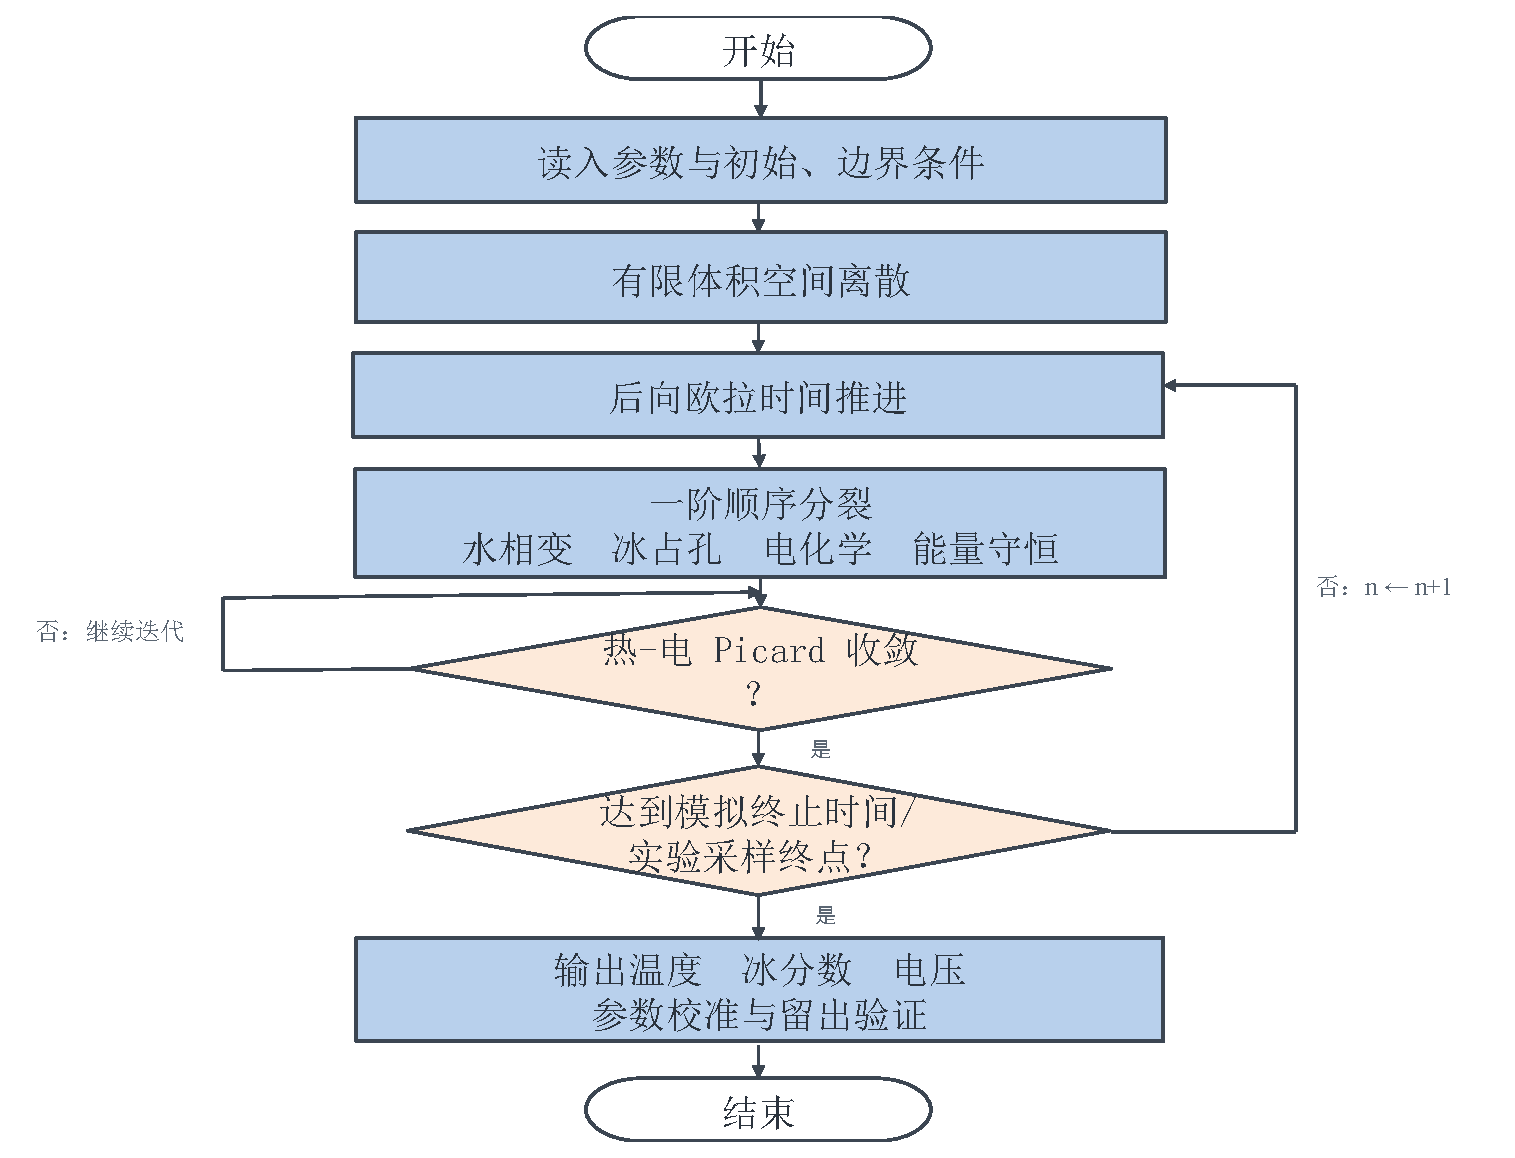
\includegraphics[width=.7\textwidth]{问题一解决问题流程图 (3).eps}
\caption{问题一：一维单电池瞬态自冷启动模型数值求解与验证流程图}
\label{F4-1}
\end{figure}

\subsection{一维单电池瞬态自冷启动模型的建立}
根据前述分析，低温冷启动与常温运行的根本差异在于水–冰相变及冰积累对传质、电化学反应和热过程的反馈作用。因此，本文以题目给出的常温一维模型为基础，在保留氢氧传输、电荷守恒、产水、能量守恒及电压模型基本结构的同时，将水相扩展为水蒸气、液态水和固态冰三相，并进一步引入冰占孔、催化层冰覆盖、膜水冻结以及相变潜热等低温机制。

此外，考虑到实际单电池在短时冷启动过程中两侧双极板具有不可忽略的热惯性，本文在原五层膜电极组件 MEA 的质量传输域之外，将两侧双极板纳入热传递计算域，形成“五层质量传输域—七层热传递域”的一维瞬态冷启动模型。该处理既保持题目给出的电化学与传质框架，又能够更完整地描述低温环境下单电池的实际升温过程。模型区域及双极板处理方式与现有推导保持一致。

\subsubsection{求解区域、基本假设及初边界条件}
\begin{itemize}
\renewcommand{\labelitemi}{$\blacktriangleright$}
\item \textbf {求解区域}

以膜电极厚度方向为 $x$ 轴，原始质量传输和电化学反应区域依次由阳极气体扩散层、阳极催化层、质子交换膜、阴极催化层和阴极气体扩散层构成，即
\begin{equation}
\Omega = \Omega_{\text{aGDL}} \cup \Omega_{\text{aCL}} \cup \Omega_{\text{PEM}} \cup \Omega_{\text{cCL}} \cup \Omega_{\text{cGDL}}.
\tag{4-1}
\end{equation}
各功能层及双极板厚度如表\ref{B4-1}所示。

\begin{table}[htbp]
    \centering
    \caption{各功能层厚度参数}
    \label{B4-1}
    \setlength{\tabcolsep}{24pt}  % 默认是6pt，这里调到24pt。如果觉得还不够宽，可以继续调大。
    \renewcommand{\arraystretch}{1.5} % 增加行高（垂直高度）
    
    \begin{tabular}{l c r} % l:左对齐 c:居中 r:右对齐
        \toprule
        \textbf{功能层} & \textbf{符号} & \textbf{厚度} \\
        \midrule
        阳极双极板       & \(L_{\text{BP}}\)  & 2.0 mm     \\
        阳极气体扩散层   & \(L_{\text{GDL}}\) & 150 \(\mu\)m \\
        阳极催化层       & \(L_{\text{aCL}}\) & 3.4 \(\mu\)m \\
        质子交换膜       & \(L_{\text{PEM}}\) & 12 \(\mu\)m  \\
        阴极催化层       & \(L_{\text{cCL}}\) & 11.3 \(\mu\)m \\
        阴极气体扩散层   & \(L_{\text{GDL}}\) & 150 \(\mu\)m \\
        阴极双极板       & \(L_{\text{BP}}\)  & 2.0 mm     \\
        \bottomrule
    \end{tabular}
\end{table}

 由此，五层 MEA 的总厚度为
\begin{equation}
L_{\text{MEA}} = 2L_{\text{GDL}} + L_{\text{aCL}} + L_{\text{PEM}} + L_{\text{cCL}} = 326.7 \, \mu\text{m}.
\tag{4-2}
\end{equation}

 将上述区域记为 \(\Omega_{\text{MEA}}\)。氢气、氧气及水的迁移和电化学反应均在该区域内求解。为考虑双极板的储热和导热作用，将热传递区域进一步扩展为
\begin{equation}
\Omega_T = \Omega_{\text{aBP}} \cup \Omega_{\text{MEA}} \cup \Omega_{\text{cBP}},
\tag{4-3}
\end{equation}
\begin{equation}
L_{\text{cell}} = 2L_{\text{BP}} + L_{\text{MEA}} = 4.3267 \, \text{mm}.
\tag{4-4}
\end{equation}

 为保持题目给定五层模型的原坐标形式，我们依旧取阳极 GDL 外侧为 \(x = 0\)，则阳极双极板位于
\begin{equation}
-L_{\text{BP}} \leq x \leq 0,
\tag{4-5}
\end{equation}
 阴极双极板位于
\begin{equation}
L_{\text{MEA}} \leq x \leq L_{\text{MEA}} + L_{\text{BP}}.
\tag{4-6}
\end{equation}

 需要强调的是，双极板在本文中仅扩展热计算区域。其内部不设置气体、水和电化学反应源项，反应气体仍由 GDL 外侧的等效流道边界进入 MEA，而不沿厚度方向穿过致密双极板。因此，气体和水的外边界与热传递域的外边界并不重合。

 根据附件给出的双极板厚度、密度与比热容，两侧双极板对应的单位面积热容为
\begin{equation}
C_{A,\text{BP}} = 2 \times 0.002 \times 1980 \times 766 = 6066.72 \, \text{J m}^{-2}\text{K}^{-1}.
\tag{4-7}
\end{equation}


\item \textbf {基本假设}

\renewcommand{\labelenumi}{\arabic{enumi}.}

 在题目常温参考模型基本假设的基础上，为使低温模型具有明确的物理边界，并避免引入过多不可识别参数，作如下补充假设：

\begin{enumerate}
    \item GDL 与 CL 均视为连续、均匀的多孔介质，PEM 采用题给膜模型；双极板视为连续、均匀致密固体；
    \item 仅考虑沿膜电极厚度方向的传质与传热，忽略面内非均匀性；
    \item 反应气体满足理想气体状态方程；
    \item 催化层内采用平均电化学反应速率，反应电流沿催化层厚度均匀分布；
    \item 外部加载电流密度 \(j(t)\) 为已知输入；
    \item 冰为静止、刚性的固相，不发生宏观迁移，只能通过冻结、融化、凝华和升华生成或消失；
    \item 在 GDL 和 CL 中，液态水与冰共同占据原始孔隙，冰生成后固定于当前位置；
    \item 水的三类相变均采用有限速率非平衡模型，相变方向由局部温度、饱和状态和当前相库存共同确定；
    \item 初始孔隙液态水、孔隙水蒸气及冰均取零，PEM 保留附件给定的初始膜含水量；
    \item 十种相变过程采用统一的一阶有限速率框架，不额外引入成核等待或 JMAK 型结晶动力学；
    \item 双极板内只考虑储热和导热，不发生水迁移、相变和电化学反应；
    \item BP/GDL 界面采用理想热接触，温度及法向热流连续，不另设置热接触电阻；
    \item 双极板电学上作为理想集流体处理，原模型中的面积比接触电阻 \(R_c\) 保持不变，不重复设置板体附加接触电阻；
    \item 含双极板模型的环境对流边界作用于两侧 BP 外表面，MEA 与双极板初温均等于环境温度。
\end{enumerate}

 这一处理使模型在保持一维性的同时，将真正影响短时冷启动的水--冰相变、冰堵和热惯性纳入统一框架。

\item \textbf {初始条件}

 温度、总含水量及反应气体初始状态分别满足
\begin{align}
\begin{cases}
T(x,0)= T_0,  m_w(x,0) = m_{w,0}(x),\\
c_{\text{H}_2}(x,0)=c_{\text{H}_2,0}(x),  c_{\text{O}_2}(x,0) = c_{\text{O}_2,0}(x). \tag{4-8}
\end{cases}
\end{align}

 对于 \(-20\,^\circ\text{C}\) 和 \(-25\,^\circ\text{C}\) 两种实验工况，分别取
\begin{equation}
T_0 = 253.15\,\text{K}, \qquad T_0 = 248.15\,\text{K}.
\tag{4-9}
\end{equation}

 含双极板模型中，该初始温度同时赋予 MEA 和两侧 BP。初始孔隙液态水及冰满足
\begin{equation}
m_l(x,0) = 0, \qquad m_i(x,0) = 0.
\tag{4-10}
\end{equation}

 PEM 初始膜含水量取附件给定的$\lambda_0 = 3$， 相应未冻束缚水质量浓度为$38.7 \times 3 = 116.1\,\text{kg}\,\text{m}^{-3}$。

 阳、阴极均采用干气入口，因此孔隙初始水蒸气取零；初始气体浓度根据 \(p = 101325\,\text{Pa}\)、入口气体组成及理想气体状态方程计算。

\item \textbf {边界条件}

气体方面，阳极和阴极 GDL 外边界的氢气、氧气浓度由入口压力、温度和组成确定，各相邻功能层界面满足质量通量连续。水传输方面，GDL 外侧按干气入口处理，液态水与冰的法向通量均为零，各功能层之间保持水通量连续。

热传递方面，含 BP 模型的环境对流边界移至两侧双极板外表面，而 BP/GDL 内部界面仅施加温度连续和热流连续条件。电荷方面，外部给定的总电流密度 \(j(t)\) 经双极板集流后作用于 MEA；由于不单独求解 BP 电势，因此 GDL 外边界仍施加相同的电流密度条件。


\end{itemize}


\subsubsection{三相水相变与质量守恒}
常温参考模型仅区分水蒸气和液态水，无法描述冰的生成及其累积过程。为此，将局部总含水量进一步划分为水蒸气、液态水和固态冰三部分，从质量守恒、相态转化以及膜水输运三个层次建立三相水模型。

\begin{itemize}
\renewcommand{\labelitemi}{$\blacktriangleright$}
\item \textbf {三相水变量及冰体积分数}

 记 \(m_v(x,t)\)、\(m_l(x,t)\) 和 \(m_i(x,t)\) 分别为单位控制体总体积内水蒸气、液态水和固态水的质量浓度，则有
\begin{equation}
m_w(x,t) = m_v(x,t) + m_l(x,t) + m_i(x,t). 
\tag{4-11}
\end{equation}

 其中下标 \(i\) 专指冰相。液态水和冰所占据的控制体体积分数分别定义为
\begin{equation}
\theta_l = \frac{m_l}{\rho_l}, \qquad \theta_i = \frac{m_i}{\rho_i}.
\tag{4-12}
\end{equation}

 附件参数取 $\rho_l = 990\text{kg m}^{-3}$,  $\rho_i = 920\text{kg m}^{-3}$。

 对第 \(i\) 个一维控制体，题目要求的局部冰体积分数可直接表示为
\begin{equation}
\varepsilon_{\text{ice},i}(t) = \frac{V_{\text{ice},i}(t)}{V_{\text{cell},i}} = \frac{\Delta x_{\text{ice},i}(t)}{\Delta x_i} = \theta_i(x_i, t) = \frac{m_i(x_i, t)}{\rho_i}. 
\tag{4-13}
\end{equation}


 进一步以干燥状态初始孔隙率 \(\varepsilon_0\) 为基准，定义液相饱和度和冰相饱和度
\begin{equation}
s_l = \frac{\theta_l}{\varepsilon_0} = \frac{m_l}{\rho_l \varepsilon_0}, \qquad s_i = \frac{\theta_i}{\varepsilon_0} = \frac{m_i}{\rho_i \varepsilon_0}. 
\tag{4-14}
\end{equation}

 其中附件1给出的 GDL、aCL 和 cCL 初始孔隙率分别为 0.8、0.3916 和 0.4207。液态水与冰共同占据孔隙后，可供气体传输的剩余孔隙率为
\begin{equation}
\varepsilon_g = \varepsilon_0 - \theta_l - \theta_i = \varepsilon_0(1 - s_l - s_i).
 \tag{4-15}
\end{equation}

 因此模型状态必须满足如下物理条件：
\begin{equation}
s_l \geq 0, \qquad s_i \geq 0, \qquad s_l + s_i \leq 1, \qquad 0 \leq \varepsilon_g \leq \varepsilon_0. 
\tag{4-16}
\end{equation}



\item \textbf {三相质量守恒}

 设 \(J_v\) 和 \(J_l\) 分别表示水蒸气和液态水沿 \(x\) 方向的质量通量。由于冰被视为静止固相，其宏观质量通量满足 \(J_i = 0\)。

 分别记冷凝、蒸发、冻结、融化、凝华和升华速率为
\[
r_{\text{cond}}, \quad r_{\text{evap}}, \quad r_{\text{frz}}, \quad r_{\text{mlt}}, \quad r_{\text{dep}}, \quad r_{\text{sub}},
\]
单位均为 \(\text{kg m}^{-3}\text{s}^{-1}\)。同时记 \(S_{\text{prod}}\) 为阴极电化学反应产生水的体积源项。

 对三相分别建立质量守恒方程。水蒸气满足
\begin{equation}
\frac{\partial m_v}{\partial t} = -\frac{\partial J_v}{\partial x} - r_{\text{cond}} + r_{\text{evap}} - r_{\text{dep}} + r_{\text{sub}}. \tag{4-17}
\end{equation}

 液态水满足
\begin{equation}
\frac{\partial m_l}{\partial t} = -\frac{\partial J_l}{\partial x} + r_{\text{cond}} - r_{\text{evap}} - r_{\text{frz}} + r_{\text{mlt}} + S_{\text{prod}}. \tag{4-18}
\end{equation}

 固态冰不发生宏观迁移，其质量变化完全来自相变：
\begin{equation}
\frac{\partial m_i}{\partial t} = r_{\text{frz}} - r_{\text{mlt}} + r_{\text{dep}} - r_{\text{sub}}. \tag{4-19}
\end{equation}

 将（4-17）--（4-19）相加，六个内部相变项相互抵消，可得
\begin{equation}
\frac{\partial(m_v + m_l + m_i)}{\partial t} = -\frac{\partial(J_v + J_l)}{\partial x} + S_{\text{prod}}. \tag{4-20}
\end{equation}

 令
\[
N_w = J_v + J_l, \qquad S_w = S_{\text{prod}},
\]
结合（4-11）即有
\begin{equation}
\frac{\partial m_w}{\partial t} = -\frac{\partial N_w}{\partial x} + S_w. \tag{4-21}
\end{equation}

 可见，所建立的三相模型与题目常温模型中的总水守恒方程严格相容，相变只改变水在气、液、固三相之间的分配，并不改变水的总质量。



\item \textbf {电化学产水}

 水仅由阴极催化层的氧还原反应生成，阴极氧还原反应的产水化学方程式为：
\begin{equation}
\ce{O2 + 4H+ + 4e- -> 2H2O}. \tag{4-22}
\end{equation}
根据备注一有，
\begin{equation}
S_{\text{prod}} = S_w = \frac{M_w j}{2F L_{\text{cCL}}}, \qquad x \in \Omega_{\text{cCL}}, \tag{4-23}
\end{equation}

 其他区域取 \(S_w = 0\)。其中
\[
M_w = 0.018 \, \text{kg mol}^{-1}, \qquad F = 96485 \, \text{C mol}^{-1}.
\]

 本题将电化学生成水首先计入阴极 CL 的液态水，再由有限速率相变模型重新进行相态分配。

\item \textbf {水蒸气扩散及饱和状态}


 由于 \(m_v\) 是按控制体总体积定义的蒸气质量浓度，而真正参与气相扩散的是孔隙气相中的浓度，故定义$c_v = m_v/\varepsilon_g$ 。

 水蒸气扩散通量与储存方程写为
\begin{equation}
J_v = -D_{v,\text{eff}} \frac{\partial c_v}{\partial x}, \qquad \frac{\partial(\varepsilon_g c_v)}{\partial t} = -\frac{\partial J_v}{\partial x} + S_v. \tag{4-24}
\end{equation}

 因此，当孔隙率随冰和液态水动态变化时，不能简单用 \(\partial m_v/\partial x\) 代替气相浓度梯度。阳极和阴极参考水蒸气扩散系数分别取$8.69 \times 10^{-5}$、 $2.48 \times 10^{-5} \, \text{m}^2\text{s}^{-1}$，
并根据局部温度及 \(\varepsilon_g^{1.5}\) 进行修正。

 零下环境中，过冷液态水表面和冰表面的平衡蒸气压并不相同。因此分别采用液水面和冰面的 Buck 关系。令$T_c = T - 273.15$，
则液水面饱和蒸气压为
\begin{equation}
p_{\text{sat},l} = 611.21 \exp\left[ \left(18.678 - \frac{T_c}{234.5}\right) \frac{T_c}{257.14 + T_c} \right],
\tag{4-25}
\end{equation}
冰面饱和蒸气压为
\begin{equation}
p_{\text{sat},i} = 611.15 \exp\left[ \left(23.036 - \frac{T_c}{333.7}\right) \frac{T_c}{279.82 + T_c} \right], \qquad T < T_f. \tag{4-26}
\end{equation}

 对应的单位总体积饱和蒸气含量分别为
\begin{equation}
m_{\text{sat},l} = \frac{\varepsilon_g M_w p_{\text{sat},l}}{RT}, \qquad m_{\text{sat},i} = \frac{\varepsilon_g M_w p_{\text{sat},i}}{RT}. \tag{4-27}
\end{equation}

 其中 \(m_{\text{sat},l}\) 用于气-液过程，\(m_{\text{sat},i}\) 用于气-冰过程，从而避免低温条件下将两种不同平衡界面混为一体。




\item \textbf {气-液、液-固和气-固的有限速率相变}

 记
\[
[z]_+ = \max(z, 0)
\]
和
\[
\mathbf{1}_{z} = 
\begin{cases} 
1, & z > 0, \\ 
0, & z = 0.
\end{cases}
\]
 则气-液相变速率写为
\begin{equation}
r_{\text{cond}} = k_c [m_v - m_{\text{sat},l}]_+, \tag{4-28}
\end{equation}
\begin{equation}
r_{\text{evap}} = k_e [m_{\text{sat},l} - m_v]_+ \mathbf{1}_{m_l > 0}. \tag{4-29}
\end{equation}

 液态水与冰之间的冻结、融化过程分别满足
\begin{equation}
r_{\text{frz}} = k_f m_{\text{free}} \left[ \frac{T_f - T}{T_f} \right]_+, \tag{4-30}
\end{equation}
\begin{equation}
r_{\text{mlt}} = k_m m_i \left[ \frac{T - T_f}{T_f} \right]_+. \tag{4-31}
\end{equation}

 对于孔隙水，
\[
m_{\text{free}} = m_l;
\]
{\color{red} 对于膜内束缚水，考虑一定比例的非冻结膜水，有
\[
m_{\text{free}} = [m_l - W_\lambda \lambda_{\text{nf}}]_+,
\]
 其中
\[
W_\lambda = \frac{\rho_{\text{PEM}} M_w}{EW} = 38.7 \, \text{kg m}^{-3},
\]
 依照附件1 我们主计算取
\[
\lambda_{\text{nf}} = 3.
\]

 令局部冻结与融化的一阶速率分别为 \(a_f\)、\(a_m\)，则采用后向欧拉库存限制后，一个时间步内的实际转移量为
\begin{equation}
\Delta m_f = m_{\text{free}} \frac{\Delta t a_f}{1 + \Delta t a_f}, \qquad \Delta m_m = m_i \frac{\Delta t a_m}{1 + \Delta t a_m}. \tag{4-32}
\end{equation}

 该形式可以保证相变转移量不超过供体相当前库存。

 当 \(T < T_f\) 时，气-固相变满足
\begin{equation}
r_{\text{dep}} = k_d [m_v - m_{\text{sat},i}]_+, \qquad r_{\text{sub}} = k_s [m_{\text{sat},i} - m_v]_+ \mathbf{1}_{m_i > 0}. \tag{4-33}
\end{equation}

 当 \(T \geq T_f\) 时，模型关闭气-冰直接相变，由融化过程描述冰相的消失。

 为保证有限时间步下相变过程不产生负库存，实际计算中按“气-液—气-冰—液-冰”的顺序进行相态更新。以气-液过程为例：
\begin{equation}
\Delta m_c = [m_v - m_{\text{sat},l}]_+ \frac{\Delta t k_c}{1 + \Delta t k_c},
\tag{4-34}
\end{equation}
\begin{equation}
\Delta m_e = \min\left(m_l, [m_{\text{sat},l} - m_v]_+ \frac{\Delta t k_e}{1 + \Delta t k_e}\right).
\tag{4-35}
\end{equation}

 气-冰过程采用相同的库存约束思想。各次相变均从供体相减去相同质量并加入受体相，因此局部相变过程中严格保持水质量守恒。}


\item \textbf {PEM内膜水输运和膜-CL水交换}

 PEM 中不存在独立气相孔隙，因此将 \(m_l\) 定义为未冻束缚水，将 \(m_i\) 定义为冻结膜水。膜内未冻水含量和总水含量分别为
\begin{equation}
\lambda_l = \frac{m_l}{W_\lambda}, \qquad \lambda_{\text{tot}} = \frac{m_l + m_i}{W_\lambda}, \qquad EW = 1 \, \text{kg mol}^{-1}. \tag{4-36}
\end{equation}

 膜内水通量由浓度扩散与电渗拖曳共同组成：
\begin{equation}
N_w^{\text{mem}} = -D_{w,\text{mem}} \frac{\partial m_l}{\partial x} + \frac{n_d M_w j}{F}, \qquad n_d = \frac{2.5\lambda_l}{22}. \tag{4-37}
\end{equation}

 膜水扩散系数采用
\begin{equation}
D_{w,\text{mem}} = 10^{-10} e^{2416(1/303.15 - 1/T)} \left( 2.563 - 0.33\lambda_l + 0.0264\lambda_l^2 - 0.000671\lambda_l^3 \right). \tag{4-38}
\end{equation}

{\color{red}  为避免该经验关系在低温、低含水区间外推时失去正性，数值计算设置
\[
D_{w,\text{mem}} \ge 10^{-13} \, \text{m}^2\text{s}^{-1},
\]
 该值仅作为数值保护下限。

 PEM 中冰体积分数直接定义为
\begin{equation}
\theta_{i,\text{PEM}} = \frac{m_i}{\rho_i}. \tag{4-39}
\end{equation}

 膜与相邻催化层之间采用有限速率水交换。令
\[
\ell_* = \frac{L_{\text{PEM}}}{2}, \qquad \chi = 1,
\]
 并规定正值表示水进入膜，则液态水交换量为
\begin{equation}
\Delta M_l = \chi(0.5 \, \text{s}^{-1})\ell_* W_\lambda s_l(14 - \lambda_l)\Delta t,
\tag{4-40}
\end{equation}
 水蒸气吸附/脱附量为
\begin{equation}
\Delta M_v = \chi(0.001 \, \text{s}^{-1})\ell_* W_\lambda [1 - \min(s_l, 1)](\lambda_{\text{eq}} - \lambda_l)\Delta t.
\tag{4-41}
\end{equation}

 其中水活度及对应膜平衡含水量取
\begin{equation}
a_w = \text{clip}\left\{ \frac{m_v / \varepsilon_g}{M_w p_{\text{sat},l} / (RT)}, 0, 1 \right\},
\tag{4-42}
\end{equation}
\begin{equation}
\lambda_{\text{eq}} = 0.043 + 17.81 a_w - 39.85 a_w^2 + 36 a_w^3.
\tag{4-43}
\end{equation}
 膜-CL 交换同样实施供体库存限制，并在界面两侧进行等质量增减，从而保证水质量守恒。}


\end{itemize}

\subsubsection{冰占孔效应、反应物传输及电化学反应修正}
冰的形成不仅改变局部含水状态，还会直接缩小气体输运通道、降低液态水迁移能力并覆盖催化剂活性位点。因此，需要将冰体积分数进一步反馈至孔隙率、扩散系数、液水渗透率和催化层有效反应面积中，使水–冰状态与电化学性能形成闭环耦合。

\begin{itemize}
\renewcommand{\labelitemi}{$\blacktriangleright$}
\item \textbf {有效孔隙率}

常温模型只考虑液态水占据孔隙，而冷启动过程中冰同样占据多孔空间。由（4-11），冷启动状态下剩余气相有效孔隙率为
\begin{equation}
\varepsilon_g(x,t) = \varepsilon_0 [1 - s_l(x,t) - s_i(x,t)] = \varepsilon_0 - \frac{m_l}{\rho_l} - \frac{m_i}{\rho_i}. \tag{4-44}
\end{equation}
随着冰不断生成，\(\varepsilon_g\) 单调减小，可供氢气和氧气扩散的实际通道逐渐收缩。


\item \textbf {有效气体扩散系数}

氢气和氧气扩散继续采用题目给出的 Bruggeman 型关系，并以冰修正后的 \(\varepsilon_g\) 替代常温孔隙率，即
\begin{equation}
D_{k,\text{eff}} = D_{k,\text{ref}} \left( \frac{T}{298.15} \right)^{1.5} \frac{101325}{p} \varepsilon_g^{1.5}, \qquad k = \text{H}_2, \text{O}_2. \tag{4-45}
\end{equation}

 代入（1-29）可得
\begin{equation}
D_{k,\text{eff}} = D_{k,\text{ref}} \left( \frac{T}{298.15} \right)^{1.5} \frac{101325}{p} [\varepsilon_0(1 - s_l - s_i)]^{1.5}. \tag{4-46}
\end{equation}

 参考扩散系数取
\[
D_{\text{H}_2,\text{ref}} = 1.10 \times 10^{-4} \, \text{m}^2\text{s}^{-1},
\]
\[
D_{\text{O}_2,\text{ref}} = 2.20 \times 10^{-5} \, \text{m}^2\text{s}^{-1}.
\]

 水蒸气扩散系数采用相同的孔隙率指数进行修正。由于 Bruggeman 指数为 1.5，冰堵对扩散能力具有非线性放大作用。例如在暂不考虑液态水时，若阴极 CL 中 \(s_i = 0.3\)，则扩散系数相对于无冰状态降低为
\[
(1 - 0.3)^{1.5} = 0.7^{1.5} \approx 0.586.
\]

\item \textbf {催化层有效反应面积}

冰在阴极催化层内还会覆盖反应活性位点。根据附件给出的阴极冰覆盖指数 \(n_{\text{ice}} = 3.5\)，定义局部有效电化学反应面积为
\begin{equation}
a_{\text{ec}}(x,t) = a_0[1 - s_i(x,t)]^{3.5}, \qquad x \in \Omega_{\text{cCL}}. \tag{4-46}
\end{equation}

 考虑冰分布在催化层内可能存在空间差异，先对局部面积修正因子沿 cCL 厚度进行平均，再用于修正整电池交换电流密度：
\begin{equation}
f_a = \frac{1}{L_{\text{cCL}}} \int_{\text{cCL}} (1 - s_i)^{3.5} \, \mathrm{d}x, \qquad j_{0,\text{eff}} = j_0(T_{\text{cCL}}) f_a. \tag{4-47}
\end{equation}

 由于非线性关系的存在，
\[
\langle (1 - s_i)^{3.5} \rangle \neq (1 - \langle s_i \rangle)^{3.5},
\]
因此模型直接根据局部冰状态计算有效面积，而不以平均冰饱和度代替局部修正。

\item \textbf {液态水迁移能力}

GDL 与 CL 内液态水主要受毛细压力驱动。附件给出的绝对渗透率分别为
\[
K_{\text{GDL}} = 6.2 \times 10^{-12} \, \text{m}^2, \qquad K_{\text{CL}} = 6.2 \times 10^{-13} \, \text{m}^2,
\]
对应接触角分别为 \(110^\circ\) 与 \(100^\circ\)。液态水 Darcy 通量写为
\begin{equation}
J_l = \frac{\rho_l K K_{rl}(s_l)}{\mu_l} \frac{\partial p_c}{\partial x}. \tag{4-48}
\end{equation}

采用
\[
\mu_l = 1.8 \times 10^{-3} \, \text{Pa s}, \qquad \sigma = 0.075 \, \text{N m}^{-1}, \qquad K_{rl} = s_l^3,
\]
并引入冰对液水迁移率的修正因子 \((1 - s_i)^3\)。利用
\begin{equation}
J(s_l) = 1.417s_l - 2.120s_l^2 + 1.263s_l^3 \tag{4-49}
\end{equation}
闭合毛细压力关系后，得到程序实际采用的等效液水扩散系数
\begin{equation}
D_l = \frac{K s_l^3}{\mu_l \varepsilon_0} \sigma |\cos \theta| \sqrt{\frac{\varepsilon_0}{K}} J'(s_l)(1 - s_i)^3, \qquad J_l = -D_l \partial_x m_l. \tag{4-50}
\end{equation}

因此，冰生成不仅压缩气相空间，同时也降低孔隙液态水的迁移能力。

\item \textbf {氢气、氧气质量守恒}

经上述冰占孔修正后，氢气和氧气在 GDL 和 CL 中满足
\begin{equation}
\frac{\partial(\varepsilon_g c_k)}{\partial t} = \frac{\partial}{\partial x} \left( D_{k,\text{eff}} \frac{\partial c_k}{\partial x} \right) + S_k, \qquad k = \text{H}_2, \text{O}_2. \tag{4-51}
\end{equation}

阳极催化层中氢气消耗源项为
\begin{equation}
S_{\text{H}_2} = -\frac{j}{2F L_{\text{aCL}}}, \qquad x \in \Omega_{\text{aCL}}, \tag{4-52}
\end{equation}

阴极催化层氧气消耗源项为
\begin{equation}
S_{\text{O}_2} = -\frac{j}{4F L_{\text{cCL}}}, \qquad x \in \Omega_{\text{cCL}}. \tag{4-53}
\end{equation}

其他区域相应源项均取零。

由（4-44）--（4-50）可知，冰累积首先降低 \(\varepsilon_g\)，继而降低 \(D_{\text{O}_2,\text{eff}}\)，最终使阴极 CL 中氧气浓度下降。这一传质链条构成冰堵引起浓差极化增强的重要物理机制。

\item \textbf {电荷守恒及电化学反应}

电子电流密度 \(i_s\)、质子电流密度 \(i_m\) 与外部加载电流密度满足
\begin{equation}
i_s + i_m = j(t). \tag{4-54}
\end{equation}

其中 GDL 仅承担电子传导，PEM 仅承担质子传导，催化层通过电化学反应实现电子电流与质子电流之间的转换。按照题目给出的平均反应假设，阳极和阴极催化层中的体积反应电流密度分别为
\begin{equation}
\dot{i}_{v,a} = \frac{j}{L_{\text{aCL}}}, \qquad \dot{i}_{v,c} = \frac{j}{L_{\text{cCL}}}. \tag{4-55}
\end{equation}

（4-55）同时用于氢气消耗、氧气消耗及阴极产水速率的计算。

本模型不再单独求解电子电势和质子电势偏微分方程，而采用给定总电流、催化层均匀体积反应以及膜电阻积分构成约化电化学模型。

附件 2 同时提供电流与两种单位的电流密度，其中
\[
j_{\text{A/m}^2} = 10^4 j_{\text{A/cm}^2}.
\]

由于附件中部分电流值与附件 1 给出的 25 cm\(^2\) 活性面积不能一致反推，因此正式计算直接以附件 2 的 A/m\(^2\) 电流密度列（此列是将原先A/cm\(^2\) 电流密度E列$*10000$换算得到的）作为输入，不再利用总电流除以 25 cm\(^2\) 二次换算，以避免引入额外数据矛盾。

\end{itemize}


\subsubsection{能量守恒与低温热效应}
冷启动过程中，电池温度由电化学反应产热、相变潜热、内部导热、双极板储热及外界对流散热共同决定。与常温模型相比，本节重点增加水–冰相变热效应和双极板瞬态热惯性。

\begin{itemize}
\renewcommand{\labelitemi}{$\blacktriangleright$}
\item \textbf {含相变热的一维能量守恒}

{\color{red} 完整热域内局部温度满足
\begin{equation}
(\rho c_p)_{\text{eff}} \frac{\partial T}{\partial t} = \frac{\partial}{\partial x} \left( k_{\text{eff}} \frac{\partial T}{\partial x} \right) + \dot{q}_{\text{gen}} + \dot{q}_{\text{pc}} + \dot{q}_{\text{ads}}. \tag{4-56}
\end{equation}}

问题一研究自冷启动过程，不施加额外电加热，因此
\[
\dot{q}_{\text{aux}} = 0.
\]

在双极板区域不存在电化学反应及水相变化，因而
\[
\dot{q}_{\text{gen}} = \dot{q}_{\text{pc}} = \dot{q}_{\text{ads}} = 0.
\]

双极板满足独立的瞬态导热方程
\begin{equation}
\rho_{\text{BP}} c_{p,\text{BP}} \frac{\partial T}{\partial t} = \frac{\partial}{\partial x} \left( k_{\text{BP}} \frac{\partial T}{\partial x} \right), \qquad x \in \Omega_{\text{aBP}} \cup \Omega_{\text{cBP}}. \tag{4-57}
\end{equation}

由此，双极板并非简单附加一个静态热阻，而是通过时间导数项显式参与冷启动过程中的热量储存与释放。

\item \textbf {等效体积热容}

对于 GDL 等不含独立离聚物相的多孔层，等效体积热容按固相、气相、液态水和冰相体积分数加权：
\begin{equation}
(\rho c_p)_{\text{eff}} = (\rho c_p)_s(1 - \varepsilon_0) + (\rho c_p)_g \varepsilon_g + (\rho c_p)_l \theta_l + (\rho c_p)_i \theta_i. \tag{4-58}
\end{equation}

CL 中另外考虑体积分数为 0.3 的离聚物，因此其固体骨架体积分数取
\[
1 - \varepsilon_0 - 0.3.
\]

PEM 则按离聚物主体叠加未冻水和冰相热容处理。

附件给出的典型体积热容包括
\[
\rho_i c_{p,i} = 920 \times 2050,
\]
\[
\rho_l c_{p,l} = 990 \times 4182,
\]
以及离聚物、GDL 骨架、CL 骨架和双极板相应材料参数。

双极板不进行孔隙相体积分数加权，直接采用
\[
\rho_{\text{BP}} = 1980 \, \text{kg m}^{-3}, \qquad c_{p,\text{BP}} = 766 \, \text{J kg}^{-1}\text{K}^{-1},
\]
\begin{equation}
(\rho c_p)_{\text{BP}} = 1.51668 \times 10^6 \, \text{J m}^{-3}\text{K}^{-1}. \tag{4-59}
\end{equation}

于是两侧双极板合计单位面积热容以及单电池完整热域单位面积热容分别为
\[
C_{A,\text{BP}} = 2 L_{\text{BP}} (\rho c_p)_{\text{BP}} = 6066.72 \, \text{J m}^{-2}\text{K}^{-1},
\]
\begin{equation}
C_{A,\text{cell}}(t) = C_{A,\text{BP}} + \int_{\Omega_{\text{MEA}}} (\rho c_p)_{\text{eff}}(x,t) \, \mathrm{d}x. \tag{4-60}
\end{equation}

其中 MEA 部分热容随局部水、冰状态变化，而双极板热容由固定材料参数决定。


\item \textbf {含冰状态下的导热系数}

对于多孔层内部，各相导热系数按体积分数作并联加权：
\begin{equation}
k_{\text{layer}} = k_s(1 - \varepsilon_0) + k_g \varepsilon_g + k_l \theta_l + k_i \theta_i. \tag{4-61}
\end{equation}

附件给出的主要参数为
\[
k_i = 2.3 \, \text{W m}^{-1}\text{K}^{-1}, \qquad k_l = 0.6 \, \text{W m}^{-1}\text{K}^{-1},
\]
GDL 固体骨架导热系数取 0.3，CL 骨架取 0.27，离聚物取 0.24，双极板取
\[
k_{\text{BP}} = 95 \, \text{W m}^{-1}\text{K}^{-1}.
\]

若从单电池整体尺度考察沿厚度方向的等效导热系数，则不同层之间按串联热阻计算：
\begin{equation}
k_{\text{eff}} = \frac{\sum\limits_i \delta_i}{\sum\limits_i (\delta_i / k_i)}. \tag{4-62}
\end{equation}

需要强调的是，数值求解时仍保留各层局部 \(k\) 值，式（1-43）主要用于整体热阻解释，而不以单一均匀 \(k_{\text{eff}}\) 取代七层材料分布。

在 BP/GDL 界面 \(x = x_\Gamma\)，采用理想热接触条件：
\begin{equation}
T(x_\Gamma^-, t) = T(x_\Gamma^+, t), \qquad -k_- \left.\frac{\partial T}{\partial x}\right|_{x_\Gamma^-} = -k_+ \left.\frac{\partial T}{\partial x}\right|_{x_\Gamma^+}. \tag{4-63}
\end{equation}

即界面处温度和法向热流连续，而两侧温度梯度允许由于材料导热系数不同而发生跃变。

\item \textbf {电化学反应热}

为避免分别计算反应热、活化热和欧姆热，将电化学产生的总热量统一写为
\begin{equation}
\dot{q}_{\text{gen}} = \frac{j(E_{\text{th}} - V_{\text{cell}})}{L}. \tag{4-64}
\end{equation}

 其中
\[
E_{\text{th}} = 1.48 \, \text{V}, \qquad L = L_{\text{MEA}}.
\]
该热源均匀施加在五层 MEA 热域内，双极板中不设置此项。其沿 MEA 厚度积分得到单位面积热流$j(E_{\text{th}} - V_{\text{cell}})$ 。


\item \textbf {水–冰相变潜热}

冷凝、冻结和凝华释放热量，而蒸发、融化和升华吸收热量。因此，相变体积热源统一写为
\begin{equation}
\dot{q}_{\text{pc}} = L_c(r_{\text{cond}} - r_{\text{evap}}) + L_f(r_{\text{frz}} - r_{\text{mlt}}) + L_s(r_{\text{dep}} - r_{\text{sub}}). \tag{4-65}
\end{equation}

附件1给出凝结潜热与冻结潜热分别为
\[
L_c = 2.5 \times 10^6 \, \text{J kg}^{-1},
\]
\[
L_f = 3.336 \times 10^5 \, \text{J kg}^{-1}.
\]

因此凝华或升华潜热取
\begin{equation}
L_s = L_c + L_f = 2.8336 \times 10^6 \, \text{J kg}^{-1}. \tag{4-66}
\end{equation}

对于膜端水蒸气吸附和脱附过程，根据实际接口转移量单独加入等效吸附热。对 PEM 端部控制体 \(p\)，有
\begin{equation}
\dot{q}_{\text{ads},p} = \frac{L_c \Delta M_v}{\Delta x_p \Delta t}. \tag{4-67}
\end{equation}

其中 \(\Delta M_v > 0\) 表示蒸气进入膜，\(\Delta M_v < 0\) 表示由膜脱附。最终热方程中的相变相关源项为 $\dot{q}_{\text{pc}} + \dot{q}_{\text{ads}}$ 。
这一处理使水相变化不仅改变水质量分布，也能够通过潜热重新反馈温度场。


\item \textbf {双极板外表面对流边界}

 无 BP 基线模型中，对流边界位于两侧 GDL 外表面；加入 BP 后，将环境边界移至
\[
x_L = -L_{\text{BP}}, \qquad x_R = L_{\text{MEA}} + L_{\text{BP}}.
\]

 两侧满足
\begin{equation}
-k_{\text{BP}} \frac{\partial T}{\partial n} = h(T_{\text{BP,out}} - T_{\text{amb}}), \qquad x = x_L, x_R. \tag{4-68}
\end{equation}

 其中
\[
h = 40 \, \text{W m}^{-2}\text{K}^{-1}.
\]

 对应单位活性面积的双侧对流散热功率为
\begin{equation}
q_{\text{loss},A} = h[T(x_L, t) - T_{\text{amb}}] + h[T(x_R, t) - T_{\text{amb}}]. \tag{4-69}
\end{equation}

 若两侧表面温度近似相同，则有
\[
q_{\text{loss},A} \approx 2h(T - T_{\text{amb}}),
\]
我们不能在整体能量平衡中遗漏任意一侧环境散热。

\item \textbf {双极板导热热阻与热惯性}

为比较双极板自身导热热阻和环境对流热阻，对单侧 BP 定义等效传热系数
\[
\frac{1}{U} = \frac{L_{\text{BP}}}{k_{\text{BP}}} + \frac{1}{h},
\]
\[
\frac{L_{\text{BP}}}{k_{\text{BP}}} = 2.1053 \times 10^{-5} \, \text{m}^2\text{K W}^{-1},
\]
\begin{equation}
U \approx 39.97 \, \text{W m}^{-2}\text{K}^{-1}. \tag{4-70}
\end{equation}

 由于
\[
\frac{1}{h} = 0.025 \, \text{m}^2\text{K W}^{-1},
\]
BP 自身厚度方向导热热阻仅约为单侧对流热阻的 0.084\%。这说明双极板内部导热温降较小，但并不意味着其热容量可以忽略。相反，在几十秒尺度冷启动过程中，较大的单位面积热容量会显著影响温升速率。因此，本文仍通过（4-69）显式求解 BP 瞬态储热，而不将其简单等效为稳态热阻。


\item \textbf {双极板热容量级诊断}


为独立判断双极板热惯性的量级是否合理，可利用实验电压、电流密度和温度估算表观单位面积热容。暂时忽略相变热、吸附热、热容变化以及内部温差，并以实验平均温度近似两侧表面温度，则在 \(t_* = 35 \, \text{s}\) 时有
\begin{equation}
C_{A,\text{app}} \approx \frac{\int_0^{t_*} [j(t)(E_{\text{th}} - V_{\text{exp}}(t)) - 2h(T_{\text{exp}}(t) - T_{\text{amb}})] \, \mathrm{d}t}{T_{\text{exp}}(t_*) - T_0}. \tag{4-71}
\end{equation}

 由现有实验数据计算，\(-20^\circ\text{C}\) 与 \(-25^\circ\text{C}\) 工况对应的表观面热容约为
\[
6117.77, \qquad 6309.90 \, \text{J m}^{-2}\text{K}^{-1},
\]
与两侧 BP 理论面热容
\[
6066.72 \, \text{J m}^{-2}\text{K}^{-1}
\]
处于同一量级。这一结果为将双极板热质量纳入瞬态模型提供了量级支持，但该估算仅作为结构合理性诊断，不用于反向拟合双极板物性参数。

\end{itemize}

\subsubsection{冰影响下的单电池电压模型}
低温冷启动时，冰不仅通过堵塞孔隙限制氧气输运，还会覆盖催化层活性区域，并使部分膜水冻结，从而分别影响活化极化、欧姆极化和浓差极化。因此，在保持题给常温电压模型总体形式不变的基础上，将前述水–冰状态引入各极化项，实现冰状态到输出电压的动态反馈。

\begin{itemize}
\renewcommand{\labelitemi}{$\blacktriangleright$}
\item \textbf {电池总电压}

 单电池电压由可逆电压减去活化、欧姆和浓差三类损失：
\begin{equation}
V_{\text{cell}} = E_{\text{rev}} - \eta_{\text{act}} - \eta_{\text{ohm}} - \eta_{\text{con}}. \tag{4-72}
\end{equation}

 因此，冰并不以独立“冰损失项”的形式直接叠加，而是通过改变局部气体浓度、交换电流密度、膜质子电导率和极限电流密度进入原有三类极化损失。

\item \textbf {可逆电压}

 采用简化 Nernst 方程：
\begin{equation}
E_{\text{rev}} = 1.229 - 8.5 \times 10^{-4}(T - 298.15) + \frac{RT}{2F} \ln \left[ \left( \frac{p_{\text{H}_2}}{p_0} \right) \left( \frac{p_{\text{O}_2}}{p_0} \right)^{1/2} \right], \tag{4-73}
\end{equation}

 其中
\[
p_0 = 101325 \, \text{Pa}.
\]
\(p_{\text{H}_2}\) 和 \(p_{\text{O}_2}\) 分别取阳极和阴极催化层局部气体分压。冰通过式（1-29）—式（1-37）改变反应气体浓度，因此会间接作用于 \(E_{\text{rev}}\)，但这一作用相对于对三类极化损失的影响较弱。


\item \textbf {活化损失及冰覆盖修正}

交换电流密度首先按照 Arrhenius 关系进行温度修正：
\begin{equation}
j_0(T) = j_{0,\text{ref}} \exp \left[ -\frac{E_a}{R} \left( \frac{1}{T} - \frac{1}{298.15} \right) \right], \tag{4-74}
\end{equation}

 其中
\[
E_a = 67000 \, \text{J mol}^{-1}.
\]

 低温状态下，再利用式（1-33）中催化层有效反应面积因子得到
\[
j_{0,\text{eff}} = j_0(T_{\text{cCL}}) f_a.
\]

 由此，活化极化采用简化 Butler--Volmer 关系
\begin{equation}
\eta_{\text{act}} = \frac{RT_c}{\alpha F} \operatorname{arsinh} \left( \frac{j}{2j_{0,\text{eff}}} \right), \qquad \alpha = 0.5. \tag{4-75}
\end{equation}

 随着冰在 cCL 中累积，\(f_a\) 减小，进而使 \(j_{0,\text{eff}}\) 下降；在相同外部电流密度下，所需活化过电位随之增加。因此，（4-75）给出了“冰覆盖—有效反应面积减少—活化损失增加”的定量表达。



\item \textbf {欧姆损失及膜水冻结修正}

 欧姆损失主要来自质子交换膜和面积比接触电阻。考虑 PEM 内水冰状态存在空间差异，对局部膜电阻沿厚度积分：
\begin{equation}
\eta_{\text{ohm}} = j \left[ \int_{\text{PEM}} \frac{\mathrm{d}x}{\kappa_{\text{pem,eff}}(x)} + R_c \right]. \tag{4-76}
\end{equation}

 其中
\[
R_c = 0.01 \, \Omega\text{cm}^2 = 10^{-6} \, \Omega\text{m}^2.
\]

 未冻结膜水含量
\[
\lambda_l = \frac{m_l}{W_\lambda}
\]

 决定膜的本征质子电导率。采用 Springer 关系：
\begin{equation}
\kappa_{\text{pem}} = (0.5139\lambda_l - 0.326)e^{1268(1/303.15 - 1/T)}. \tag{4-77}
\end{equation}

 进一步考虑膜中冰相对质子传输通道的阻断作用，定义有效质子电导率
\begin{equation}
\kappa_{\text{pem,eff}} = \kappa_{\text{pem}}(1 - \theta_{i,\text{PEM}}). \tag{4-78}
\end{equation}

 由此，膜欧姆性能受到两方面共同影响：一方面，水冻结后可参与质子传导的未冻水减少；另一方面，冰体积分数增加又进一步降低有效导电通道。两种作用共同推动 \(\eta_{\text{ohm}}\) 增大。


\item \textbf {浓差损失及冰堵修正}

 阴极供氧受限所造成的浓差损失表示为
\begin{equation}
\eta_{\text{con}} = -\frac{RT}{4F} \ln \left( 1 - \frac{j}{j_{\text{lim}}} \right). \tag{4-79}
\end{equation}

 题目给出的极限电流密度为
\begin{equation}
j_{\text{lim}} = \frac{4 F D_{\text{O}_2,\text{eff}} C_{\text{O}_2,\text{cCL}}}{L_{\text{diff}}}. \tag{4-80}
\end{equation}

 其中 \(C_{\text{O}_2,\text{cCL}}\) 由氧气质量守恒方程求得，\(L_{\text{diff}}\) 为阴极侧等效扩散距离。

 由于 $D_{\text{O}_2,\text{eff}} \propto \varepsilon_g^{1.5}$ ，
冰占孔将同时降低有效扩散系数和阴极催化层氧气浓度，从而使 \(j_{\text{lim}}\) 持续降低。当外部加载电流逐渐接近冰堵压低后的极限电流时，
（4-79）中的对数项迅速增大，造成浓差过电位快速上升，这对应冷启动过程中严重冰堵所引起的电压骤降。

 实际数值模型进一步按照阴极 CL 中心至 GDL 外表面的分层扩散阻力求取等效传质能力，以
\[
R_D = \sum \frac{\Delta x}{D_{\text{O}_2,\text{eff}}}
\]
替代单一均匀介质近似中的
\[
\frac{L_{\text{diff}}}{D_{\text{O}_2,\text{eff}}}.
\]

 若某时刻出现$\frac{j}{j_{\text{lim}}} \geq 1$，
则说明在当前冰堵和供氧状态下给定电流已经超过局部物理传质极限，模型将该状态判定为无效，而不通过人为截断 \(j / j_{\text{lim}}\) 的方式维持虚假的可行电压。

 最后，单电池电压模型与前述三相水、冰占孔及热模型形成完整闭环：外部电流驱动电化学反应并产生水和热；水在低温下发生三相转化形成冰；冰通过孔隙率、扩散系数、反应面积和膜质子电导率改变各类极化损失；电压变化又直接改变反应产热 \(\dot{q}_{\text{gen}}\)，进而反馈局部温度和后续相变过程。由此构成一维单电池瞬态自冷启动模型的完整耦合体系。

\end{itemize}


\subsection{模型的数值求解与参数校准}
上一节建立的冷启动模型同时包含气体传输、水的三相迁移与相变、冰堵反馈、热量传递以及电化学反应等过程，各状态变量之间存在较强的非线性耦合。其中，水和冰的累积会改变有效孔隙率及传质参数，进而影响电池电压；电压又通过反应产热作用于温度场，而温度进一步决定水-冰相变方向及速率。针对这一特点，本文采用有限体积法进行空间离散，并结合隐式时间推进、顺序分裂和 Picard 迭代完成各物理场的耦合求解。在此基础上，利用 \(-20^\circ\text{C}\) 实验数据进行参数校准，并将所得参数直接用于 \(-25^\circ\text{C}\) 工况，以检验模型对不同初始温度的预测能力。

\subsubsection{模型离散与耦合求解}

 考虑到 MEA 各功能层厚度及物理性质差异较大，本文采用控制体中心有限体积法对厚度方向进行分层离散。对于任意守恒变量 \(\phi\)，第 \(j\) 个控制体的离散形式统一写为
\begin{equation}
\frac{\mathrm{d}\phi_j}{\mathrm{d}t} = \frac{J_{j-1/2} - J_{j+1/2}}{\Delta x_j} + S_j, \tag{4-81}
\end{equation}

 其中，\(\Delta x_j\) 为控制体厚度，\(J_{j-1/2}\) 和 \(J_{j+1/2}\) 分别为左右界面通量，\(S_j\) 为相应源项。该形式使相邻控制体公共界面上的质量通量或热流以等量反向形式进入两侧控制体，从而保证离散层面的局部守恒。

 根据催化层和质子交换膜厚度较小、状态梯度较大的特点，对这些区域适当加密。最终计算中，aGDL、aCL、PEM、cCL 和 cGDL 分别划分为 16、6、12、8、16 个控制体，五层 MEA 共设置 58 个质量传输节点；在含双极板热模型中，两侧 BP 各增加 8 个温度控制体，因此完整热域共包含 74 个温度节点。气体和水仍只在原 MEA 网格内求解，双极板仅参与热传导和储热计算。

对于跨材料界面的热传递，为正确反映不同材料之间的串联热阻，相邻控制体 \(p\) 和 \(q\) 的界面导度取为
\begin{equation}
G_{pq} = \left( \frac{\Delta x_p}{2k_p} + \frac{\Delta x_q}{2k_q} \right)^{-1}, \tag{4-82}
\end{equation}

 相应热流为
\begin{equation}
q_{p\to q} = G_{pq}(T_p - T_q). \tag{4-83}
\end{equation}

 对于最外侧双极板控制体，还需同时计及半个控制体的导热热阻和环境对流热阻，其边界等效导度写为
\begin{equation}
G_b = \left[ \frac{\Delta x_b}{2k_{\text{BP}}} + \frac{1}{h} \right]^{-1}. \tag{4-84}
\end{equation}

 气体扩散、水蒸气扩散、膜水扩散及热传导均采用类似的界面通量处理方式，从而保证材料界面处传输通量连续。

 时间方向采用一阶向后欧拉格式。对于一般形式的储存变量 \(u\)，其离散形式为
\begin{equation}
\frac{b^{n+1}u^{n+1} - b^n u^n}{\Delta t} = F(u^{n+1}), \tag{4-85}
\end{equation}

 其中 \(b\) 表示与孔隙率或热容有关的容量系数。由于冰和液态水的累积会导致孔隙率随时间变化，因此气体储存项采用 \(\varepsilon_g c\) 的完整形式进行离散，而不将 \(\varepsilon_g\) 视为常数，以避免破坏冰占孔条件下的质量守恒。膜内电渗拖曳采用守恒隐式迎风形式，各扩散和传热子问题离散后形成的三对角线性方程组直接求解。
 
 由于模型中各物理过程之间具有明显的先后依赖关系，本文采用顺序分裂方法完成一个时间步内的状态更新。首先根据附件 2 的电流密度曲线插值得到当前时刻的加载电流，并根据法拉第定律在阴极催化层中加入反应产水；随后依次计算孔隙液态水迁移、膜水扩散及电渗拖曳，并处理膜—催化层间的水交换；在此基础上求解水蒸气扩散，并依次完成气–液、气–冰和液–冰相变。完成水相更新后，根据新的液水和冰分布重新计算有效孔隙率及气体扩散系数，进而求解氢气、氧气传输。最后固定当前时间步的水相和气体状态，对温度、电池电压及反应产热进行迭代求解。

在最后的热--电耦合过程中，由于电化学产热满足
\begin{equation}
\dot{q}_{\text{gen}} = \frac{j(E_{\text{th}} - V_{\text{cell}})}{L}, \tag{4-86}
\end{equation}

而 \(V_{\text{cell}}\) 又与温度、气体浓度、膜含水量及冰覆盖状态有关，因此采用 Picard 迭代更新温度和电压。设第 \(k\) 次迭代温度为 \(T^{(k)}\)，则依次计算
\begin{equation}
T^{(k)} \to V_{\text{cell}}^{(k)} \to \dot{q}_{\text{gen}}^{(k)} \to T^{(k+1)}. \tag{4-87}
\end{equation}

当
\begin{equation}
\max_j \left| T_j^{(k+1)} - T_j^{(k)} \right| < 10^{-7} \, \text{K} \tag{4-88}
\end{equation}

\noindent 时认为当前时间步收敛。每一时间步最多迭代 30 次；若达到最大迭代次数后温度增量仍大于 \(10^{-6} \, \text{K}\)，则判定当前计算未收敛并停止推进。由此，本文的数值算法可概括为
\begin{figure}[!h]
\centering
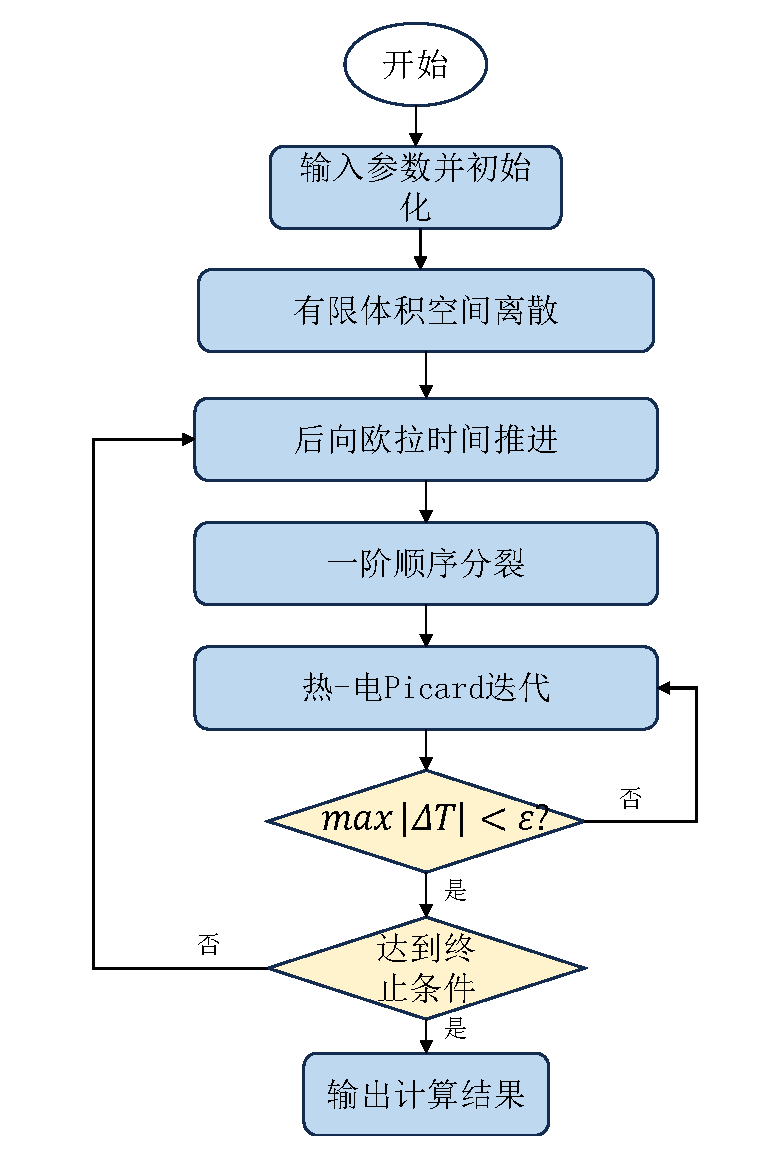
\includegraphics[width=.5\textwidth]{算法流程图222.eps}
\caption{数值算法流程图}
\label{F111}
\end{figure}


为兼顾参数搜索效率和最终计算精度，参数校准首先采用较粗网格及最大时间步 0.05 s 搜索参数范围，随后在上述 58 个 MEA 控制体的加密网格上，以最大时间步 0.0125 s 进行参数精修，最终正式结果同样采用该精细配置。由于实验数据每 0.2 s 给出一个采样点，各采样区间内部按照最大时间步进行均匀细分，使数值解能够准确落在实验采样时刻。

模型输出的单电池平均温度采用完整热域的厚度平均，即
\begin{equation}
\bar{T}(t) = \frac{\sum\limits_j T_j(t) \Delta x_j}{\sum\limits_j \Delta x_j}. \tag{4-89}
\end{equation}

对于含双极板模型，上式遍历全部 74 个热控制体，其结果记为 \(\bar{T}_{\text{cell}}\)。此外，为分析内部温度状态，分别定义 MEA 和双极板平均温度
\begin{equation}
\bar{T}_{\text{MEA}} = \frac{\sum\limits_{j \in \text{MEA}} T_j \Delta x_j}{L_{\text{MEA}}}, \tag{4-90}
\end{equation}
\begin{equation}
\bar{T}_{\text{BP}} = \frac{\sum\limits_{j \in \text{aBP} \cup \text{cBP}} T_j \Delta x_j}{2 L_{\text{BP}}}, \tag{4-91}
\end{equation}

三者满足
\begin{equation}
\bar{T}_{\text{cell}} = \frac{L_{\text{MEA}} \bar{T}_{\text{MEA}} + 2 L_{\text{BP}} \bar{T}_{\text{BP}}}{L_{\text{cell}}}. \tag{4-92}
\end{equation}

 题目要求的最大冰体积分数则由各 MEA 控制体局部冰量计算：
\begin{equation}
\varepsilon_{\text{ice,max}}(t) = \max_{j \in \text{MEA}} \frac{m_{i,j}(t)}{\rho_i}. \tag{4-93}
\end{equation}

除上述主要输出外，计算过程中同时记录孔隙冰、膜冰以及各类相变累计量，用于后续分析不同区域的冻结特征。

\subsubsection{参数校准与留出验证}

冷启动模型中包含冷凝、蒸发、冻结、融化、凝华和升华六类相变过程。由于附件 2 仅提供单电池电压和平均温度实验数据，并未给出局部冰量或相变速率的直接观测，如果同时将多个相变系数作为自由参数拟合，容易产生严重的参数相关性，使不同参数组合得到相近的电压和温度曲线而对应完全不同的内部冰状态。为降低这一不可识别性，本文将六种相变速率系数固定为前述基准值，仅选择对电压响应影响直接且具有明确电化学意义的参考交换电流密度 \(j_{0,\text{ref}}\) 作为待校准参数，即
\begin{equation}
\boldsymbol{\theta} = [j_{0,\text{ref}}]. \tag{4-94}
\end{equation}

因此，参数校准的目的并非利用实验数据重新拟合水-冰相变动力学，而是在保持低温相变模型结构不变的前提下确定电化学模型中的有效交换电流尺度。该处理可以减少自由参数数量，避免利用有限的 \(V-T\) 数据过度调整冰相动力学。

为进一步区分参数拟合能力和模型预测能力，将附件 2 中 \(-20^\circ\text{C}\) 和 \(-25^\circ\text{C}\) 两组实验数据分别作为校准集和验证集。首先利用 \(-20^\circ\text{C}\) 工况 \(0 \sim 35 \, \text{s}\) 内全部 176 个采样点校准 \(j_{0,\text{ref}}\)，而 \(-25^\circ\text{C}\) 数据在优化过程中完全不参与参数更新。完成校准后，将所得参数保持不变，直接用于 \(-25^\circ\text{C}\) 初始温度下的模型计算。由此形成
\[
-20^\circ\text{C} \implies \text{参数校准},
\]
\[
-25^\circ\text{C} \implies \text{留出验证}.
\]
与分别针对两个温度工况单独拟合相比，该处理能够更客观地评价模型对初始温度变化的预测能力。


由于 \(j_{0,\text{ref}}\) 的合理范围可能跨越多个数量级，令$x = \log_{10} j_{0,\text{ref}} $
并在对数空间中完成参数搜索。为了同时利用实验电压和温度信息，又避免二者量纲及数值尺度差异导致某一变量在目标函数中占据主导，按照题目给出的相对误差思想构造联合目标函数
\begin{equation}
J(x) = \frac{1}{N} \sum_{r=1}^N \left[ \left( \frac{V_r - V_{r,\text{exp}}}{V_{r,\text{exp}}} \right)^2 + \left( \frac{T_{r,C} - T_{r,\text{exp},C}}{T_{r,\text{exp},C}} \right)^2 \right], \qquad N = 176, \tag{4-95}
\end{equation}
其中，\(V_r\) 和 \(T_{r,C}\) 分别为第 \(r\) 个采样时刻的模型电压与模型摄氏温度，\(V_{r,\text{exp}}\) 和 \(T_{r,\text{exp},C}\) 为对应实验值。该目标函数同时约束电压动态和温升过程，使所得到的参数不只服务于单一输出变量。
参考交换电流密度的搜索范围取
\[
10^{-5} \leq j_{0,\text{ref}} \leq 10^3 \text{ A m}^{-2}.
\]
求解过程中先利用粗网格在整个参数范围内搜索目标函数较小的区域，再采用有界一维优化方法进行局部精修；最后在正式加密网格和 0.0125 s 最大时间步下重新计算并确定最终参数。若某一候选参数使模型出现孔隙率越界、负质量、膜电导率失效、极限电流不足或热迭代不收敛等情况，则认为该候选状态不满足模型物理约束，并在优化过程中予以排除。


 按照上述方法，含双极板主模型最终得到
\begin{equation}
j_{0,\text{ref}} = 0.10255839 \, \text{A m}^{-2}. \tag{4-96}
\end{equation}

 该参数由 \(-20^\circ\text{C}\) 工况确定，并在后续 \(-25^\circ\text{C}\) 模型计算中保持不变，不再进行二次校准。

 模型预测结果与实验数据之间的逐点相对误差按照题目定义计算：
\begin{equation}
\varepsilon_X = \frac{|X_{\text{sim}} - X_{\text{exp}}|}{|X_{\text{exp}}|} \times 100\%, \tag{4-97}
\end{equation}

 其中 \(X\) 分别取电池电压或平均温度。除逐点相对误差外，后续还通过均方根误差和平均相对误差评价整个时间序列的总体拟合水平，从而同时反映局部预测偏差和整体预测能力。


为保证所得结果并非由特定空间网格或时间步长造成，在确定最终参数后进一步进行时间步减半、空间网格加密及二者联合加密计算，并检查水质量守恒、冰相转移关系以及离散热量预算。上述检验只用于确认数值实现和离散求解的一致性，而模型对实验现象的实际预测效果仍需通过下一节的电压、温度和冰体积分数结果进行评价。

最后，本文通过有限体积离散和顺序耦合求解，将三相水迁移、冰堵、气体传输及热—电反馈统一到同一瞬态计算框架中；随后采用 \(-20^\circ\text{C}\) 工况校准唯一自由电化学参数，并以 \(-25^\circ\text{C}\) 工况进行留出验证。该处理既降低了多参数同时拟合造成的不可识别问题，也为后续从实验误差、冰量演化及模型预测能力三个方面评价冷启动模型奠定了基础。


\subsection{模型结果与实验验证}

在完成参数校准后，分别对初始温度为 \(-20\,^\circ\mathrm C\) 和 \(-25\,^\circ\mathrm C\) 的冷启动过程进行数值计算。其中，\(-20\,^\circ\mathrm C\) 工况用于参数校准，\(-25\,^\circ\mathrm C\) 工况不再调整任何参数，直接用于检验模型在不同初始温度下的预测能力。为完整评价模型性能，本文首先比较五层基线模型与实验结果，进一步分析引入双极板热惯性后的修订效果；随后结合相对误差、冰相演化、电压损失分解及时空分布，对模型预测结果及其物理合理性进行分析。

\subsubsection{模型预测结果及实验对比}

首先考察仅采用题目五层 MEA 作为热计算区域时的结果。图 4-1 给出了五层基线模型在两种初始温度下的电压、平均温度与实验采样值对比。

\begin{figure}[!h]
\centering
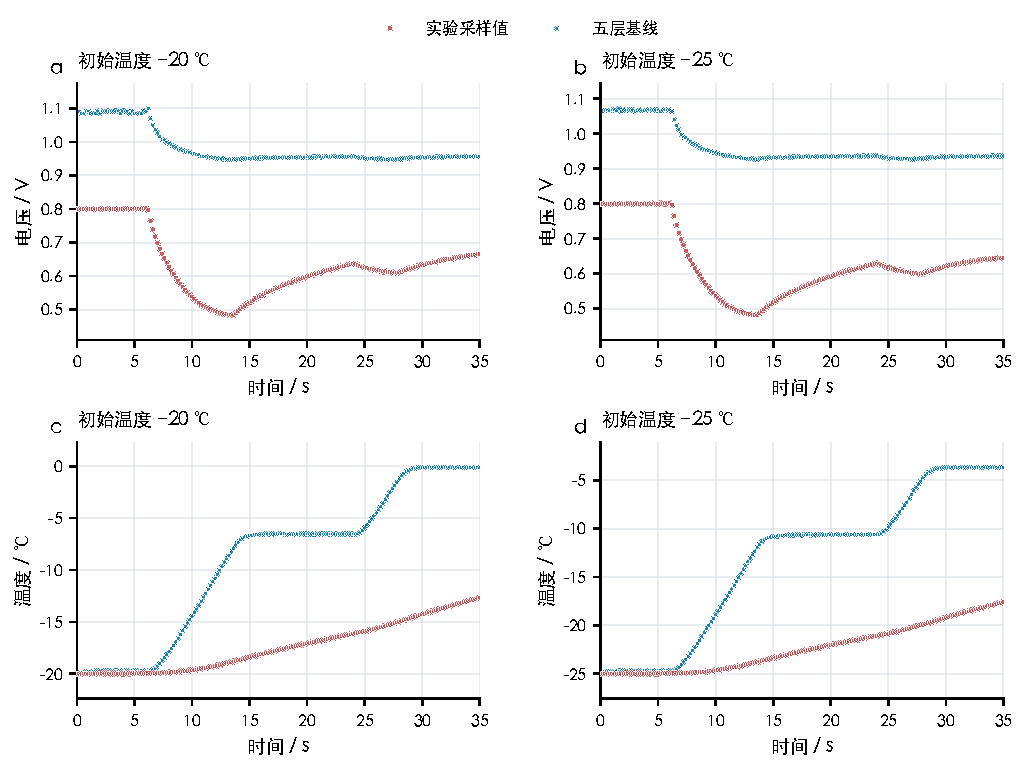
\includegraphics[width=.9\textwidth]{01_五层基线电压温度计算值与实验采样值对比.pdf}
\caption{五层基线电压温度计算值与实验采样值对比图}
\label{F4-2}
\end{figure}

由图\ref{F4-2} 可以看出，五层基线模型虽然能够反映加载电流变化后电压下降以及电池升温的基本趋势，但计算结果与实验存在明显的系统性偏差。尤其是温度响应方面，五层模型在约 \(10\sim15\,\mathrm s\) 后出现快速升温，并在 \(30\,\mathrm s\) 左右已接近 \(0\,^\circ\mathrm C\)；而实验中，\(-20\,^\circ\mathrm C\) 工况在 \(35\,\mathrm s\) 时温度仍为约 \(-12.67\,^\circ\mathrm C\)，\(-25\,^\circ\mathrm C\) 工况仍约为 \(-17.59\,^\circ\mathrm C\)。这表明只考虑 MEA 自身热容量会显著低估实际单电池的热惯性，从而高估短时冷启动过程中的升温速度。与此同时，温度预测偏差又进一步影响反应动力学和极化损失，使五层基线模型的电压始终明显高于实验值。图中这一现象说明，在几十秒量级的冷启动过程中，仅使用五层 MEA 热域不足以描述实际单电池的瞬态热响应。

考虑到单电池两侧双极板具有较大的材料体积和热容量，本文进一步将其纳入热传递区域。图 \ref{F4-3} 给出了实验值、五层基线模型及含双极板修订模型的统一对比。

\begin{figure}[!h]
\centering
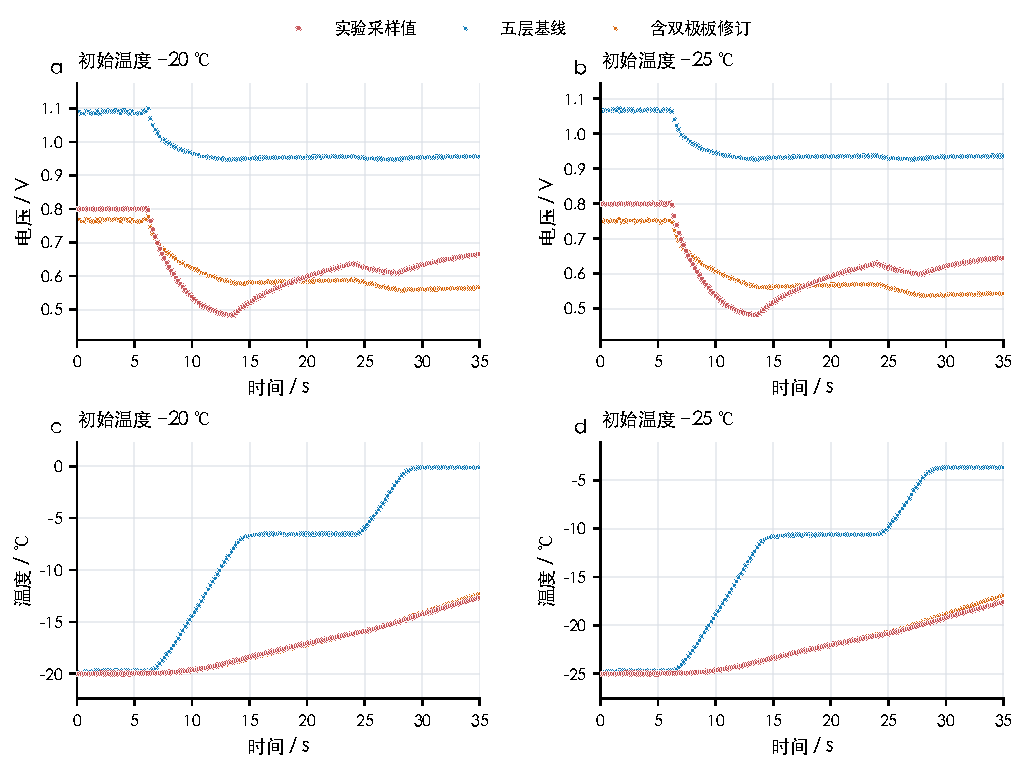
\includegraphics[width=.9\textwidth]{02_实验值五层基线与含双极板修订模型对比.pdf}
\caption{实验数据与五层基线与含双极板修订模型对比图}
\label{F4-3}
\end{figure}

由图\ref{F4-3}可见，加入双极板后模型的温升速度显著降低，与两种工况下实验温度曲线基本重合；与此同时，电压预测也由五层基线模型的明显高估修正至实验数据附近。特别是在未参与参数校准的 \(-25\,^\circ\mathrm C\) 工况下，修订模型仍能够保持与 \(-20\,^\circ\mathrm C\) 工况相近的预测精度，说明所建立模型并非只针对单一初始温度进行拟合，而具有一定的跨温度预测能力。

进一步结合表 \ref{B12} 和表 \ref{B13} 可以定量评价修订模型的预测效果。对于 \(-20\,^\circ\mathrm C\) 工况，模型温度由初始的 \(-20.00\,^\circ\mathrm C\) 上升至 \(35\,\mathrm s\) 时的 \(-12.30\,^\circ\mathrm C\)，实验值为 \(-12.67\,^\circ\mathrm C\)；对应各主要采样时刻的温度相对误差总体较小。对于 \(-25\,^\circ\mathrm C\) 留出验证工况，\(35\,\mathrm s\) 时模型预测温度为 \(-16.90\,^\circ\mathrm C\)，实验值为 \(-17.59\,^\circ\mathrm C\)，仍保持较高的一致性。全时序统计结果表明，含双极板模型在 \(-20\,^\circ\mathrm C\) 和 \(-25\,^\circ\mathrm C\) 下的温度 RMSE 分别为 \(0.1162\,^\circ\mathrm C\) 和 \(0.2323\,^\circ\mathrm C\)，MAPE 分别为 \(0.5271\%\) 和 \(0.6946\%\)；相比之下，五层基线模型的温度 RMSE 分别达到 \(9.72\,^\circ\mathrm C\) 和 \(10.62\,^\circ\mathrm C\)。因此，双极板热惯性的引入是准确描述短时冷启动温升过程的关键。


\begin{table}[htbp]
    \centering
    \caption{含双极板模型的\(-20^\circ\text{C}\) 工况模型预测与实验结果对比}
    \vspace{0.3cm}
    \label{B12}
    \renewcommand{\arraystretch}{1.5} % 增加行高，匹配原图
    \resizebox{\textwidth}{!}{ % 自动缩放表格以适应页面宽度
        \begin{tabular}{|c|c|c|c|c|c|c|c|}
            \hline
            时间/s & 实验电压/V & 模型电压/V & 电压相对误差/\% & 实验温度/\(^\circ\text{C}\) & 模型温度/\(^\circ\text{C}\) & 温度相对误差/\% & 最大冰体积分数 \\
            \hline
            0  & 0.799000 & 0.769731 & 3.663190  & -19.995355 & -20.000000 & 0.023232 & 0.000000 \\
            \hline
            5  & 0.801000 & 0.762745 & 4.775911  & -19.962098 & -19.965883 & 0.018959 & 0.000465 \\
            \hline
            10 & 0.538000 & 0.624812 & 16.136054 & -19.651712 & -19.675824 & 0.122697 & 0.002372 \\
            \hline
            15 & 0.521000 & 0.579803 & 11.286608 & -18.409761 & -18.519738 & 0.597384 & 0.012507 \\
            \hline
            20 & 0.599000 & 0.585546 & 2.246155  & -17.080544 & -17.178850 & 0.575544 & 0.029526 \\
            \hline
            25 & 0.626000 & 0.580184 & 7.318929  & -15.904149 & -15.908433 & 0.026938 & 0.049906 \\
            \hline
            30 & 0.633000 & 0.560552 & 11.445124 & -14.273271 & -14.132645 & 0.985239 & 0.074231 \\
            \hline
            35 & 0.666000 & 0.565082 & 15.152841 & -12.665591 & -12.302080 & 2.870064 & 0.099520 \\
            \hline
        \end{tabular}
    }
\end{table}


\begin{table}[htbp]
    \centering
    \caption{含双极板模型：\(-25^\circ\text{C}\) 工况模型预测与实验结果对比}
    \vspace{0.3cm}
    \label{B13}
    \vspace{0.3cm}
    \renewcommand{\arraystretch}{1.5} % 增加行高，匹配原图
    \resizebox{\textwidth}{!}{ % 自动缩放表格以适应页面宽度
        \begin{tabular}{|c|c|c|c|c|c|c|c|}
            \hline
            时间/s & 实验电压/V & 模型电压/V & 电压相对误差/\% & 实验温度/\(^\circ\text{C}\) & 模型温度/\(^\circ\text{C}\) & 温度相对误差/\% & 最大冰体积分数 \\
            \hline
            0  & 0.799000 & 0.751969 & 5.886215  & -24.995416 & -25.000000 & 0.018337 & 0.000000 \\
            \hline
            5  & 0.800000 & 0.751914 & 6.010688  & -24.962128 & -24.962845 & 0.002871 & 0.000595 \\
            \hline
            10 & 0.537000 & 0.607482 & 13.125135 & -24.645267 & -24.646270 & 0.004072 & 0.003115 \\
            \hline
            15 & 0.518000 & 0.562155 & 8.524082  & -23.380583 & -23.427279 & 0.199721 & 0.018212 \\
            \hline
            20 & 0.592000 & 0.567582 & 4.124711  & -22.032555 & -22.025768 & 0.030803 & 0.041527 \\
            \hline
            25 & 0.618000 & 0.560438 & 9.314254  & -20.846074 & -20.692829 & 0.735130 & 0.068589 \\
            \hline
            30 & 0.621000 & 0.539458 & 13.130775 & -19.201220 & -18.819982 & 1.985489 & 0.101085 \\
            \hline
            35 & 0.644000 & 0.543360 & 15.627382 & -17.587999 & -16.898513 & 3.920203 & 0.135035 \\
            \hline
        \end{tabular}
    }
\end{table}

电压预测的总体误差高于温度预测。由表 \ref{B12}和表\ref{B13} 可知，\(-20\,^\circ\mathrm C\) 工况下，模型电压在 \(10\,\mathrm s\) 和 \(15\,\mathrm s\) 分别为 \(0.6248\,\mathrm V\) 和 \(0.5798\,\mathrm V\)，实验值分别为 \(0.538\,\mathrm V\) 和 \(0.521\,\mathrm V\)；而在 \(20\,\mathrm s\) 附近二者差异明显减小。至 \(35\,\mathrm s\)，模型电压为 \(0.5651\,\mathrm V\)，实验值为 \(0.666\,\mathrm V\)。\(-25\,^\circ\mathrm C\) 工况表现出相似规律。全部采样点统计得到两种工况的电压 RMSE 分别为 \(0.0595\,\mathrm V\) 和 \(0.0608\,\mathrm V\)，MAPE 分别为 \(8.66\%\) 和 \(9.02\%\)。尽管电压误差大于温度误差，但 \(-25\,^\circ\mathrm C\) 留出工况并未出现明显误差放大，说明模型能够较稳定地预测不同初温下的总体电压水平。


\begin{figure}[!h]
\centering
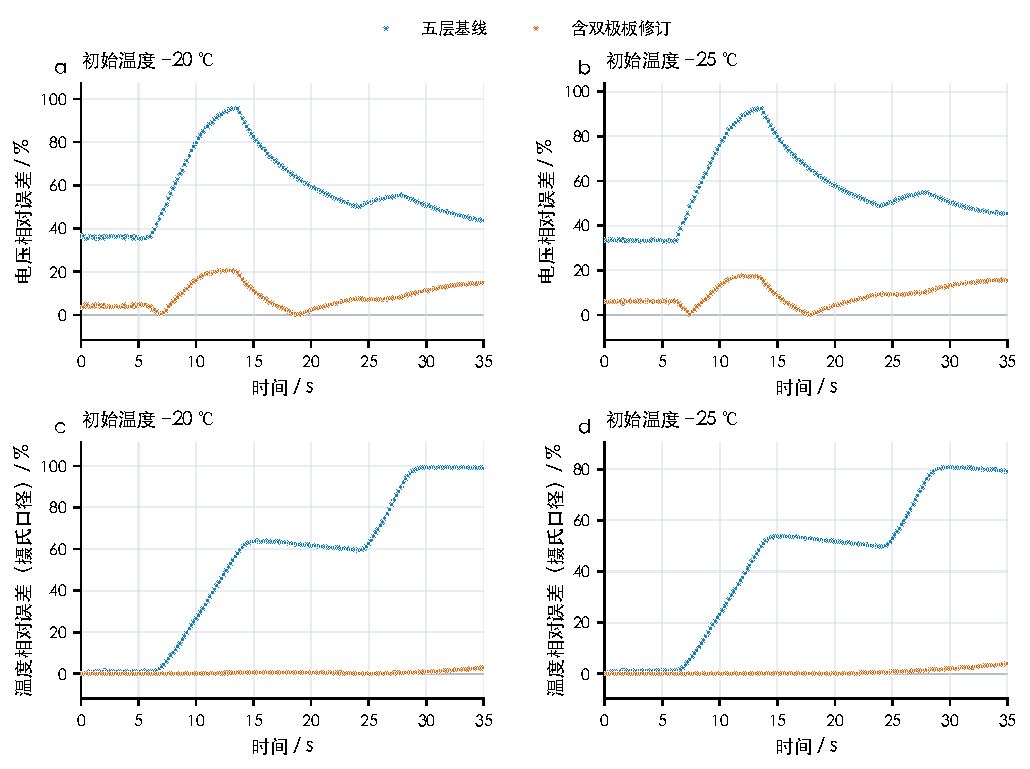
\includegraphics[width=.9\textwidth]{03_电压和温度相对误差.pdf}
\caption{电压和温度相对误差图}
\label{F4-4}
\end{figure}
图 \ref{F4-4} 进一步给出了两种热域下逐时刻的电压和温度相对误差。可以更清晰地看出模型修订前后的差异。五层基线模型在中后期的温度相对误差迅速增大，部分时段接近或达到 \(100\%\)，电压误差也长期维持在较高水平；而加入双极板后，两种初始温度下的温度相对误差在绝大部分时间内均保持较低水平，电压误差也显著下降。修订模型的电压误差在约 \(10\sim15\,\mathrm s\) 以及启动后期相对较大，表明当前模型对电压变化的总体量级能够描述，但对局部动态转折仍存在一定偏差。

从实验和模型曲线的时间位置看，这种偏差主要表现为电压谷值时刻未被完全复现。实验中，\(-20\,^\circ\mathrm C\) 和 \(-25\,^\circ\mathrm C\) 工况的最低电压分别约出现在 \(13.6\,\mathrm s\) 和 \(13.4\,\mathrm s\)；而修订模型中的最低电压分别出现在约 \(28.2\,\mathrm s\) 和 \(28.0\,\mathrm s\)。因此，现有模型对温升过程的刻画较为准确，但对电压谷值形成及恢复的动态机制仍存在一定滞后。


\subsubsection{冰相演化及其对电压变化的影响}
温度与电压的实验对比只能反映模型的宏观响应，而低温冷启动的关键内部状态是冰的生成与累积。图 \ref{F4-5} 给出了五层基线模型与含双极板修订模型在两种初始温度下的最大总冰体积分数、最大孔隙冰体积分数、最大膜相冰体积分数以及最大孔隙冰饱和度。

\begin{figure}[!h]
\centering
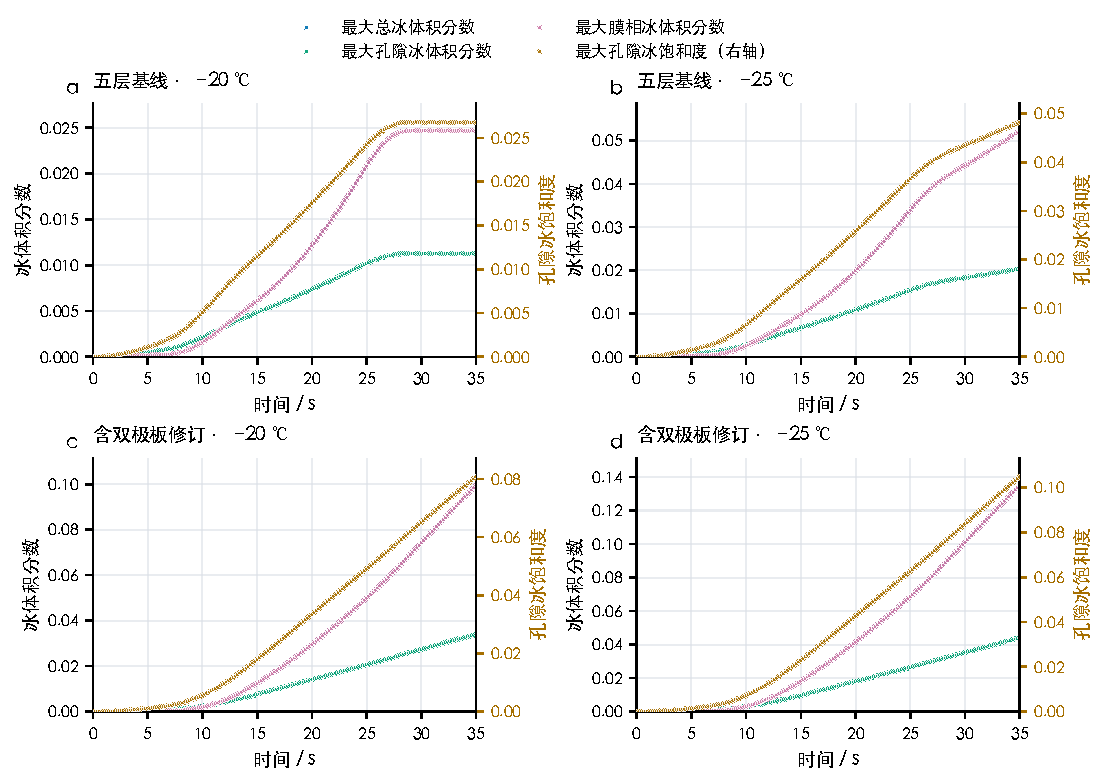
\includegraphics[width=.9\textwidth]{04_总冰孔隙冰膜相冰体积分数与孔隙冰饱和度.pdf}
\caption{总冰孔隙冰膜相冰体积分数与孔隙冰饱和度图}
\label{F4-5}
\end{figure}

由图 \ref{F4-5} 可以看出，在含双极板修订模型中，两种工况下冰量在 \(0\sim35\,\mathrm s\) 内均持续增加，且 \(-25\,^\circ\mathrm C\) 工况的冰积累始终高于 \(-20\,^\circ\mathrm C\) 工况。这与较低初始温度下液态水冻结驱动力更强、低温持续时间更长的物理规律相一致。由表 \ref{B12} 和表 \ref{B13} 可知，\(35\,\mathrm s\) 时最大总冰体积分数分别达到 \(0.0995\) 和 \(0.1350\)，即 \(-25\,^\circ\mathrm C\) 工况的最终最大冰量明显高于 \(-20\,^\circ\mathrm C\) 工况。
另一方面，图 \ref{F4-5}也说明“最大总冰体积分数”与“实际孔隙堵塞程度”并非同一概念。含双极板模型在 \(35\,\mathrm s\) 时，\(-20\,^\circ\mathrm C\) 和 \(-25\,^\circ\mathrm C\) 的最大总冰体积分数分别约为 \(9.95\%\) 和 \(13.50\%\)，而最大孔隙冰体积分数仅约为 \(3.39\%\) 和 \(4.41\%\)，对应最大孔隙冰饱和度约为 \(8.07\%\) 和 \(10.48\%\)。总冰最大值主要来源于膜内冻结水，因此不能直接把总冰体积分数解释为 GDL 或 CL 的气体孔道堵塞比例。

\begin{figure}[!h]
\centering
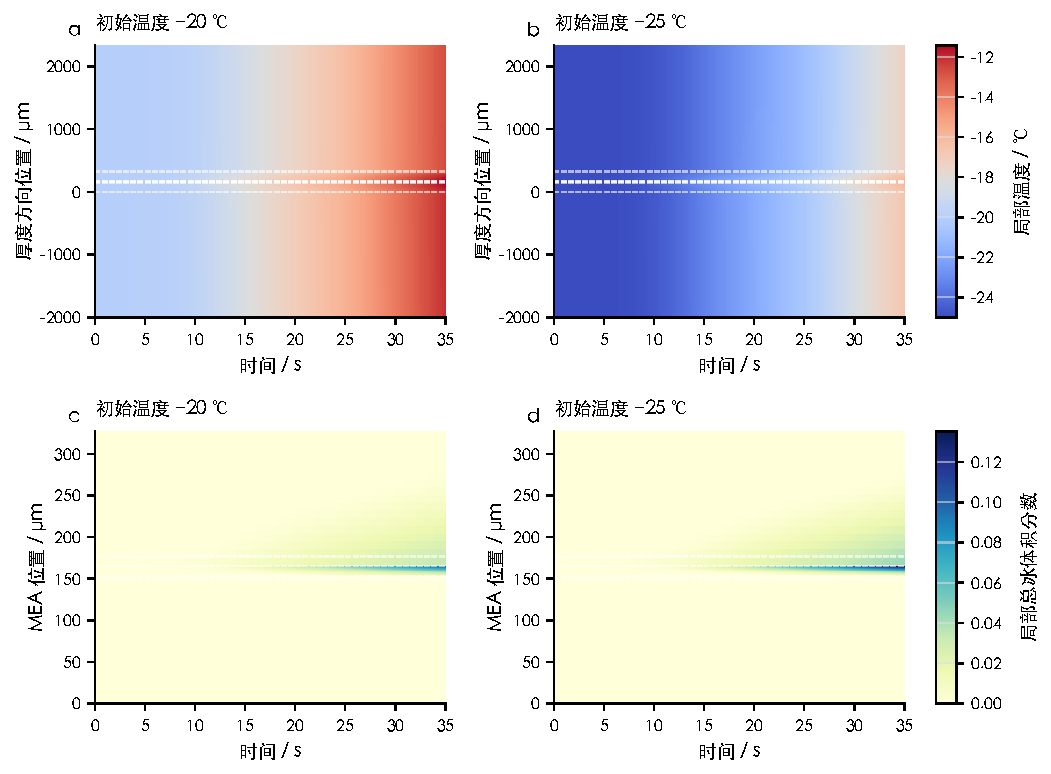
\includegraphics[width=.9\textwidth]{08_含双极板修订模型温度与结冰时空分布.pdf}
\caption{含双极板修订模型温度与结冰时空分布图}
\label{F4-6}
\end{figure}

由图 \ref{F4-6} 的温度场可以看出，含双极板后沿整个单电池厚度方向的温度分布较为平缓，其主要变化发生在时间维度；这与双极板较高的导热系数及较大的热容量相吻合。两种初温下温度均随时间持续升高，但整个 \(35\,\mathrm s\) 计算窗口内仍低于冰点。冰相空间分布则明显集中在 MEA 中部附近，主要位于 PEM 与阴极催化层邻近区域；其中 \(-25\,^\circ\mathrm C\) 工况的局部冰体积分数更高、累积范围更明显。

这一时空分布结果与图 \ref{F4-5} 相互印证：当前模型中最大冰量主要出现在膜相附近，而真正能够直接占据多孔介质孔道的孔隙冰相对较小。因此，虽然冰堵会降低有效孔隙率和氧气扩散系数，但当前 \(0\sim35\,\mathrm s\) 时间范围内电压变化并不能简单归因于“孔隙完全堵塞”。

\begin{figure}[!h]
\centering
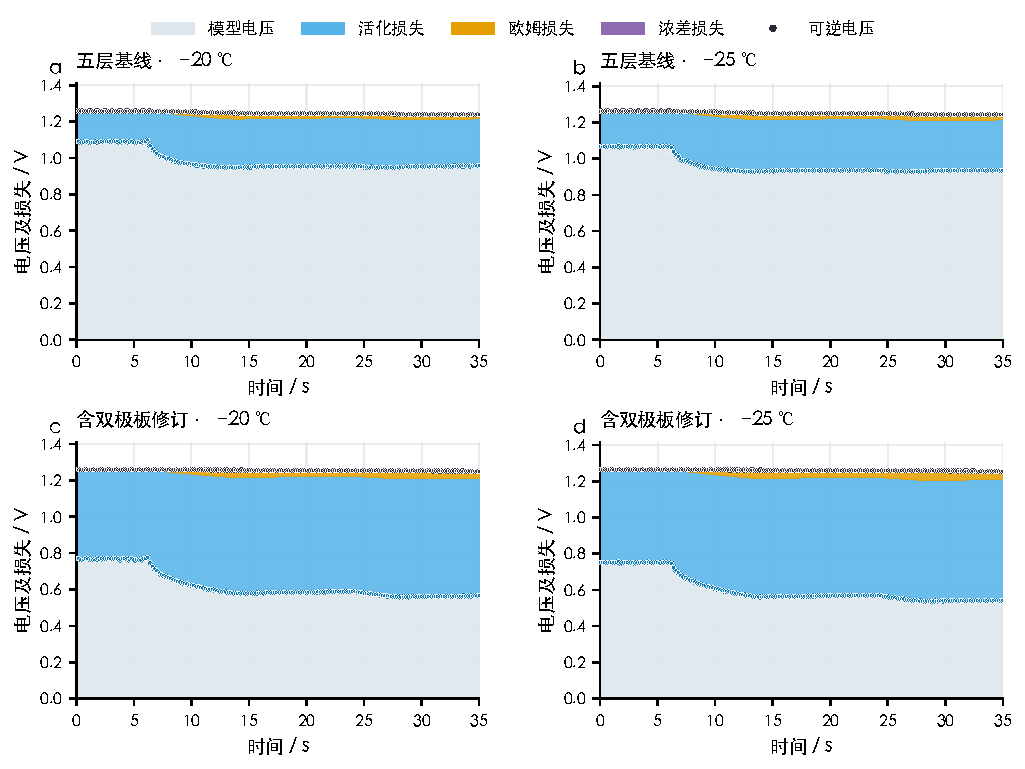
\includegraphics[width=.9\textwidth]{05_模型电压与活化欧姆浓差损失分解.pdf}
\caption{模型电压与活化欧姆浓差损失分解图}
\label{F4-7}
\end{figure}

为进一步分析电压下降机制，图 \ref{F4-7}给出了可逆电压、模型输出电压及活化、欧姆和浓差损失的分解结果。由图 \ref{F4-7} 可知，在当前模型参数与闭合关系下，三类极化损失中活化损失占主导地位，欧姆损失次之，浓差损失整体较小。随着电流加载增加，活化损失明显增大，使电池电压迅速下降；与此同时，温度升高会改善反应动力学和膜质子传导，而冰积累又通过催化层有效反应面积、膜水状态及有效扩散系数产生反向作用，因此模型电压实际上是升温有利效应与结冰不利效应共同作用的结果。

由模型计算可知，两种含双极板工况在 \(0\sim35\,\mathrm s\) 内局部温度均未超过冰点，累计融化质量为零；同时冰体积分数由图 \ref{F4-5} 可见始终保持增长。因此，当前实验中约 \(14\,\mathrm s\) 后的电压回升并非由冰融化引起，更可能是温升对电化学动力学、膜电导率等有利作用逐渐增强并超过部分冻结负面效应的综合结果。


\subsubsection{模型守恒性与结果可靠性}
除与实验数据进行外部验证外，还需检查所建立多物理场模型在数值计算中的内部一致性。图 \ref{F4-8} 给出了含双极板修订模型的水量和热量收支。

\begin{figure}[!h]
\centering
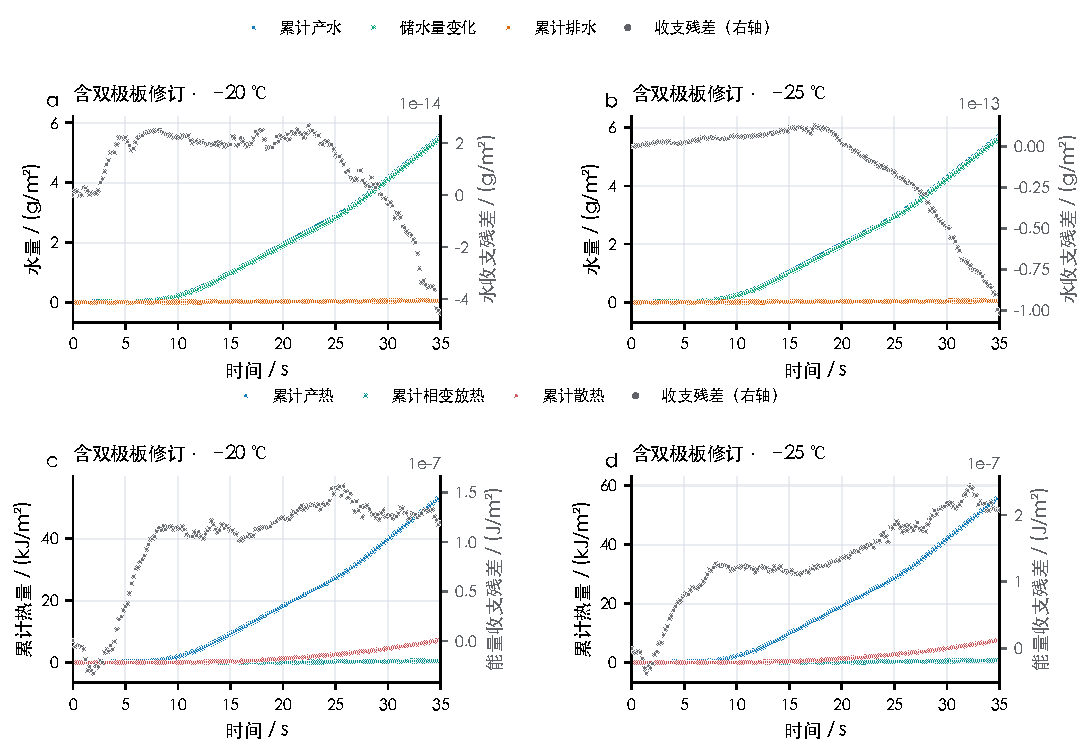
\includegraphics[width=.9\textwidth]{06_含双极板修订模型水量热量收支与守恒残差.pdf}
\caption{含双极板模型水量热量收支与守恒残差图}
\label{F4-8}
\end{figure}

由图 \ref{F4-8}(a)、(b) 可见，两种工况下累计电化学产水与域内储水量变化基本保持一致，累计排水量较小，而水量收支残差始终维持在接近机器精度的数量级；由图 \ref{F4-8}(c)、(d) 可见，累计反应产热随时间持续增加，相变热和边界散热被同步计入能量收支，能量残差同样保持在极小范围内。数值结果中，总水质量残差绝对值低于 \(1.4\times10^{-16}\,\mathrm{kg\,m^{-2}}\)，离散热量预算残差低于 \(2.5\times10^{-7}\,\mathrm{J\,m^{-2}}\)。由此说明三相质量转移、跨界面通量和热量离散在当前算法中保持了较好的守恒一致性。

进一步的网格和时间步加密检验表明，含双极板模型相对于正式工作网格的联合加密结果中，\(-20\,^\circ\mathrm C\) 与 \(-25\,^\circ\mathrm C\) 工况的电压最大差异分别仅为 \(1.78\times10^{-4}\,\mathrm V\) 和 \(2.54\times10^{-4}\,\mathrm V\)，温度最大差异分别约为 \(0.0010\,^\circ\mathrm C\) 和 \(0.0015\,^\circ\mathrm C\)。因此，电压和平均温度的数值离散误差已经远小于模型与实验之间的实际偏差，说明上述宏观结果不是由当前网格或时间步选择造成的。

需要指出的是，冰量预测的不确定性高于温度和电压。最大冰体积分数在联合加密后的变化约占正式结果峰值的 \(3\%\sim4\%\)，且冻结速率、膜非冻结水阈值以及膜—CL 水交换关系均会对冰量产生较明显影响。由于附件实验未提供局部冰量或膜含水量的直接测量，因此表\ref{B12}、表 \ref{B13} 对温度和电压的验证并不能等价为对内部冰体积分数的独立实验验证。本文所给冰量应理解为在当前相变动力学和膜水闭合条件下得到的模型预测状态，其主要作用是描述不同低温工况的结冰趋势和评价冰堵风险。

综合表 \ref{B12}、表 \ref{B13} 及图 \ref{F4-3}--图 \ref{F4-8} 可以得到：五层基线模型由于忽略双极板热质量，明显高估短时冷启动中的温升速度，进而难以正确预测电压；加入双极板热惯性后，两种初始温度下的平均温度均得到较准确预测，并使电压误差显著降低。模型进一步表明，低温越低，冰相累积越明显，其中总冰主要集中于膜及阴极催化层邻近区域，而孔隙冰占比相对较低；在当前模型下，电压损失主要受活化极化控制，温升改善与持续结冰共同决定了电压的动态变化。虽然模型仍未准确再现实验电压谷值的具体时刻，但其对热响应、电压量级及不同初温下结冰趋势具有较好的描述能力，可作为后续电堆冷启动建模与加载策略优化的单电池基础模型。
\subsection{问题一小结}
针对低温条件下氢燃料电池自冷启动过程中“产热—散热”与“产水—冻结”相互竞争的问题，本文在题目所给常温一维模型基础上，引入水蒸气、液态水和固态冰三相水描述，建立了包含冻结/融化、冷凝/蒸发及凝华/升华过程的相变模型，并通过冰体积分数动态修正有效孔隙率、气体扩散系数、催化层有效反应面积及膜质子电导率，使水冰状态能够反馈至传质过程和电化学性能。同时，将相变潜热纳入能量守恒，并进一步考虑双极板的储热与导热作用，形成“五层质量传输域—七层热传递域”的一维瞬态自冷启动模型。

在数值求解方面，采用有限体积法进行空间离散，结合后向欧拉时间推进、顺序分裂及热—电 Picard 迭代完成各物理场耦合计算；利用 \(-20\,^\circ\mathrm C\) 实验数据校准参考交换电流密度，并将所得参数直接用于 \(-25\,^\circ\mathrm C\) 工况进行留出验证。结果表明，若仅采用五层 MEA 热域，会明显低估实际单电池的热惯性，导致温升速度和电压均产生较大偏差；引入双极板后，两种工况下模型温度曲线与实验结果显著接近，\(-20\,^\circ\mathrm C\) 和 \(-25\,^\circ\mathrm C\) 工况的温度 RMSE 分别降至 \(0.1162\,^\circ\mathrm C\) 和 \(0.2323\,^\circ\mathrm C\)，电压 MAPE 分别为 \(8.66\%\) 和 \(9.02\%\)，说明模型能够较好描述不同初始温度下的整体热响应和电压变化水平。

进一步分析表明，在 \(0\sim35\,\mathrm s\) 冷启动过程中，两种工况的冰体积分数均持续增加，且 \(-25\,^\circ\mathrm C\) 工况结冰更为严重；\(35\,\mathrm s\) 时最大总冰体积分数分别约为 \(0.0995\) 和 \(0.1350\)。冰量主要集中于膜及阴极催化层邻近区域，而真正占据多孔介质孔道的孔隙冰相对较小。电压损失分解显示，当前模型中活化极化占主要部分，电压变化由升温带来的动力学改善与持续结冰造成的传质、电荷传递恶化共同决定，而不能简单归因于融冰。

此外，水量和热量收支残差均保持在极小数量级，网格和时间步加密后温度、电压变化很小，说明数值实现具有较好的守恒性与稳定性。需要指出的是，模型对实验电压谷值出现时刻仍存在一定偏差，且附件缺少局部冰量的直接测量，因此冰体积分数应视为当前相变动力学和膜水闭合条件下的模型预测状态，而非独立实验测量值。总体而言，所建立模型能够较好刻画单电池低温自冷启动过程中温度、电压与结冰状态的耦合演化，可作为后续五片电堆冷启动建模及电流加载策略优化的基础。

\section{问题二的分析与求解}
\subsection{问题描述和分析}
问题二要求在问题一单电池瞬态自冷启动模型的基础上，将研究对象扩展为由 5 片单电池串联组成的电堆，并在给定最大电流密度和累计电荷量约束下，优化恒流、线性升载和分段阶梯三类电流加载策略，以尽可能缩短电堆达到启动成功条件的时间。进一步还需确定电堆能够实现自冷启动的最低初始温度，并分析低于该温度时导致启动失败的关键单电池及原因。

与问题一相比，问题二的关键变化在于引入了电堆尺度上的热耦合与端部效应。各片单电池在相同电流密度下具有相同的反应产热和产水机制，但相邻单电池之间存在热传导，端部单电池还受到环境散热及端板热惯性的影响，因此不同位置单电池的温升速度、电压和冰积累程度可能出现差异。尤其端部单电池更容易出现温升滞后，从而成为限制整堆启动的薄弱环节。

此外，电流加载同时具有促进产热和增加产水的双重作用：提高电流有利于加快升温，但也会增加低温下的结冰风险并降低电压。因此，本文在问题一水—热—电耦合模型基础上，引入片间导热和端部热效应，建立五片电堆瞬态自冷启动模型；随后对三类加载策略进行参数优化，并通过逐步降低初始温度搜索电堆自冷启动的临界温度，从而分析不同加载方式下的启动性能及临界失效机理。
\subsection{五片电堆瞬态自冷启动模型的建立}
问题一已经建立了包含水—冰相变、冰占孔、气体输运、能量守恒及电化学极化过程的一维单电池瞬态冷启动模型。问题二在此基础上进一步考虑五片单电池串联形成电堆后的片间热传递及端部效应。由于题目假定各片反应气体分配均匀，五片单电池内部仍采用第四章建立的相同水—热—电耦合模型，其差异主要来源于堆叠方向的传热边界：相邻单电池之间通过双极板传导热量，而首尾单电池还受到端板热质量及低温环境散热的共同影响。因而，本文在单片模型之外建立电堆尺度集中参数热网络，并利用各片平均温度与原单片模型进行双向耦合。

\subsubsection{电堆结构、节点划分及基本假设}
\begin{itemize}
\renewcommand{\labelitemi}{$\blacktriangleright$}
\item \textbf {电堆结构}

沿电堆堆叠方向，从左至右依次包括左端板、左侧终端双极板、5片膜电极组件、4块内部共用双极板、右侧终端双极板以及右端板。相邻两片MEA共用一块双极板，其两侧分别服务于相邻电池，故不能按照两块独立双极板重复计算。五片电堆共包含4块内部共用双极板和2块终端流场板，共计6个板位置。其结构如图\ref{F5-1}所示。

\begin{figure}[!h]
\centering
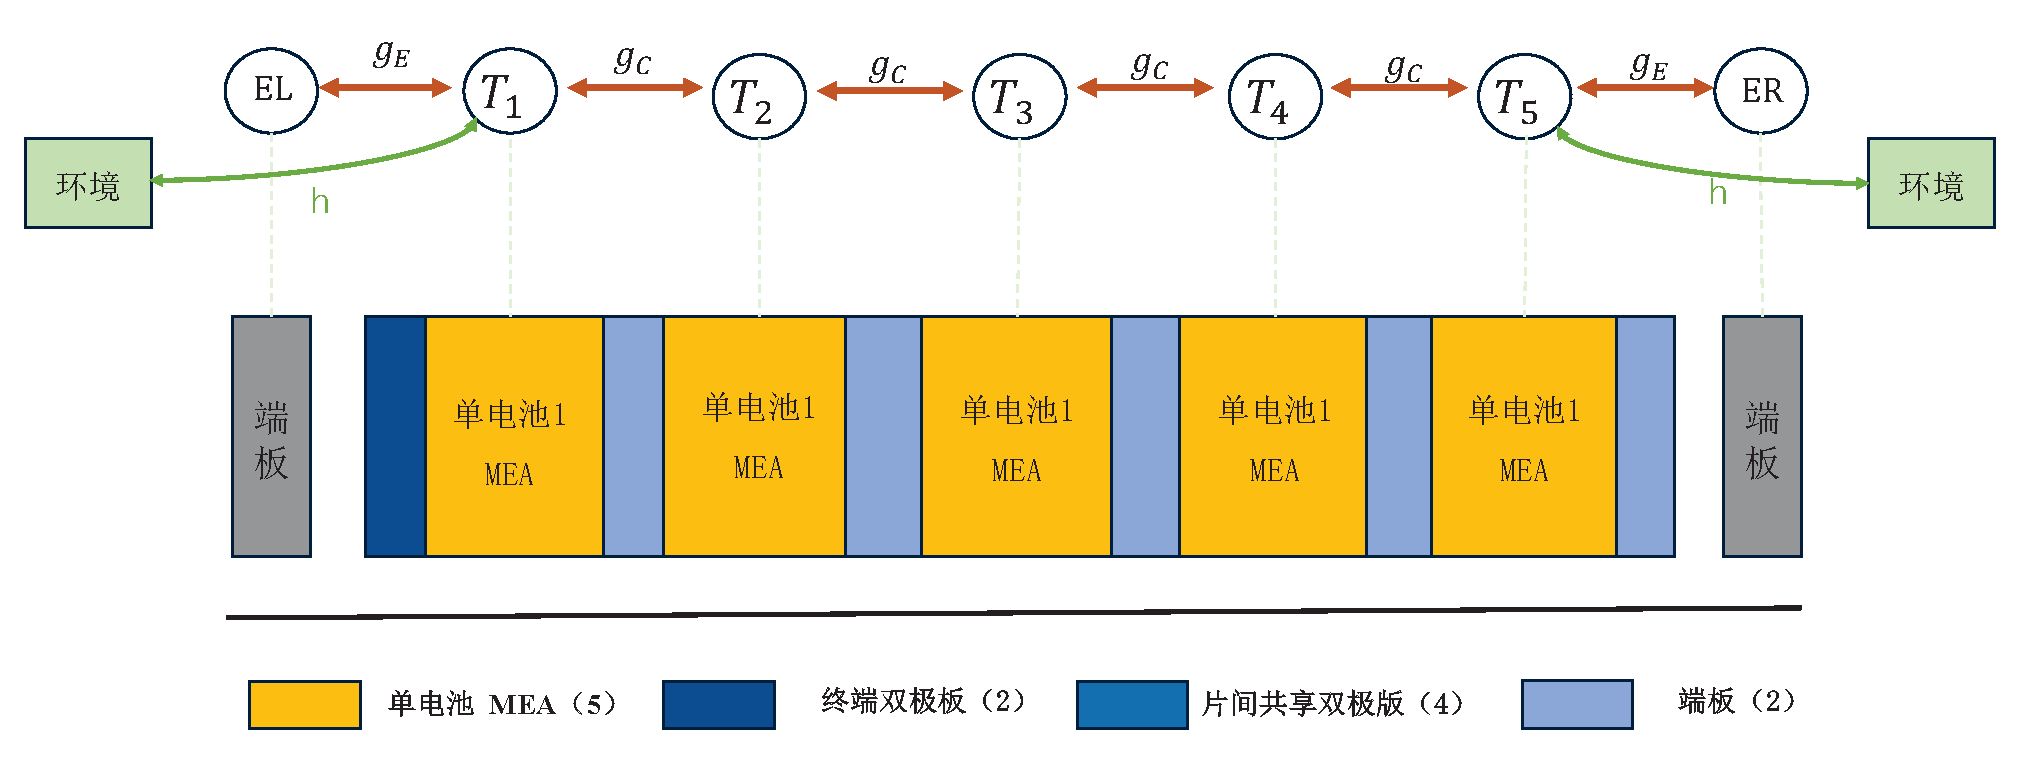
\includegraphics[width=.9\textwidth]{电堆模型.eps}
\caption{五片电堆结构及热耦合模型示意图}
\label{F5-1}
\end{figure}

问题一中的孤立单电池采用两块独立外侧双极板，而本问则按照实际共享板结构重新分配板体热容量，以避免对内部双极板热质量重复计量。


 由第四章可知，单片MEA总厚度为
\begin{equation}
L_{\text{MEA}} = 2L_{\text{GDL}} + L_{\text{aCL}} + L_{\text{PEM}} + L_{\text{cCL}} = 326.7 \, \mu\text{m}. \tag{5-1}
\end{equation}

 在电堆集中参数热网络中，以各片MEA中心作为单电池代表平面。因此，相邻两片单电池代表平面之间的距离即电池节距：
\begin{equation}
\delta = L_{\text{MEA}} + L_{\text{BP}} = 0.3267 \, \text{mm} + 2 \, \text{mm} = 2.3267 \, \text{mm}. \tag{5-2}
\end{equation}

 电堆各层的有效换热面积取题目给出的单电池截面积：
\begin{equation}
A = 25 \, \text{cm}^2 = 2.5 \times 10^{-3} \, \text{m}^2. \tag{5-3}
\end{equation}

 为兼顾端板较大的热惯性和计算效率，本文采用7节点集中参数热网络，包括5个单电池节点 \(T_k(t)\) (\(k = 1,\dots,5\)) 和2个端板节点 \(T_{\text{EL}}(t)\)、\(T_{\text{ER}}(t)\)。其连接关系为
\begin{equation}
\text{EL} \overset{g_E}{\longleftrightarrow} 1 \overset{g_c}{\longleftrightarrow} 2 \overset{g_c}{\longleftrightarrow} 3 \overset{g_c}{\longleftrightarrow} 4 \overset{g_c}{\longleftrightarrow} 5 \overset{g_E}{\longleftrightarrow} \text{ER}. \tag{5-4}
\end{equation}

 其中，\(g_c\) 为相邻单电池间单位面积热导，\(g_E\) 为端部单电池与端板之间的单位面积耦合热导。端部单电池1和5同时按照题给条件与低温环境进行对流换热。

 端板不能简单并入端部单电池作为同一等温节点。端板单位面积热容约为 \(3.95 \times 10^4 \, \text{J m}^{-2}\text{K}^{-1}\)，明显高于单电池节点热容，其与端部单电池之间的传热过程与冷启动时间处于相近时间尺度。因此若将端板和端部单电池强制等温，会忽略端板的瞬态吸热特性，并高估端部单电池的实际升温能力。源模型因此采用独立端板节点处理。


\item \textbf {基本假设}

 在问题一模型假设基础上，对电堆进一步作如下假设：

\begin{enumerate}
    \item 电堆由5片结构和材料参数相同的MEA串联组成，相邻MEA共用一块双极板，两端各设置一块终端流场板；
    \item 五片单电池串联工作并承受相同电流密度 \(j(t)\)，各片内部电化学反应、水迁移及相变方程形式相同；
    \item 反应气体在各片之间均匀分配，不考虑歧管和流道造成的气体分配差异，电堆非均匀性主要来源于端部效应及片间传热；
    \item 相邻单电池以及单电池与端板之间采用理想热接触，忽略界面接触热阻；
    \item 端板视为均匀致密固体，只参与储热和导热，不发生水迁移、相变和电化学反应；
    \item 五片电池及两块端板初始温度均为 \(T_0\)，环境温度取 \(T_{\text{amb}} = T_0\)；
\end{enumerate}

\end{itemize}

\subsubsection{片间导热及端部热效应}

\begin{itemize}
\renewcommand{\labelitemi}{$\blacktriangleright$}
\item \textbf {相邻单电池间导热}

 题目给出的相邻单电池导热功率为
\begin{equation}
\dot{Q}_{k,k+1} = \frac{k_{\text{eff}}A}{\delta} [T_k(t) - T_{k+1}(t)], \qquad k = 1, 2, 3, 4. \tag{5-5}
\end{equation}

 式中，\(k_{\text{eff}}\) 为相邻单电池代表平面之间的等效导热系数。定义相邻电池之间的单位面积热导 \(g_c\)，则有
\begin{equation}
g_c = \frac{k_{\text{eff}}}{\delta}, \qquad \dot{Q}_{k,k+1} = A g_c (T_k - T_{k+1}). \tag{5-6}
\end{equation}

 为避免将 \(k_{\text{eff}}\) 简单等同于某一材料的导热系数，本文从相邻两个 MEA 中心之间的实际串联热阻出发确定 \(g_c\)。热量从第 \(k\) 片 MEA 中心传至第 \(k+1\) 片 MEA 中心，依次经过半片 MEA、一块内部共用双极板以及另一半片 MEA。因此单位面积总热阻为
\begin{equation}
R_{\text{pitch}} = \frac{L_{\text{MEA}}/2}{k_{\text{MEA}}} + \frac{L_{\text{BP}}}{k_{\text{BP}}} + \frac{L_{\text{MEA}}/2}{k_{\text{MEA}}} = \frac{L_{\text{MEA}}}{k_{\text{MEA}}} + \frac{L_{\text{BP}}}{k_{\text{BP}}}. \tag{5-7}
\end{equation}

 于是
\begin{equation}
g_c = \frac{1}{R_{\text{pitch}}}, \qquad k_{\text{eff}} = \frac{\delta}{R_{\text{pitch}}} = \delta g_c. \tag{5-8}
\end{equation}

 其中，MEA 本身由 aGDL、aCL、PEM、cCL 和 cGDL 沿厚度方向串联，其单位面积热阻和等效贯穿导热系数分别为
\begin{equation}
R_{\text{MEA}} = \sum_j \frac{\delta_j}{k_j}, \qquad k_{\text{MEA}} = \frac{L_{\text{MEA}}}{R_{\text{MEA}}}. \tag{5-9}
\end{equation}

 在干燥初始状态下，各功能层内部按照第四章中的体积分数加权方法计算层内导热系数，结果如表\ref{B5-1}所示。

\begin{table}[htbp]
    \centering
    \caption{MEA各功能层干燥状态下的等效导热系数}
    \renewcommand{\arraystretch}{1.5} % 增加行高，匹配原图
        \label{B5-1}
    \begin{tabular}{l c l r}
        \toprule
        功能层 & 干孔隙率 \(\varepsilon_0\) & 骨架/离聚物分率 & \(k_j / (\text{W m}^{-1}\text{K}^{-1})\) \\
        \midrule
        aGDL & 0.8 & 骨架0.2 & \(0.3(0.2) + 0.1672(0.8) = 0.1938\) \\
        aCL & 0.3916 & 骨架0.3084、离聚物0.3 & \shortstack[r]{\(0.27(0.3084) + 0.24(0.3) +\) \\ \(0.1672(0.3916) = 0.2207\)} \\
        PEM & --- & 全离聚物 & \(0.2400\) \\
        cCL & 0.4207 & 骨架0.2793、离聚物0.3 & \shortstack[r]{\(0.27(0.2793) + 0.24(0.3) +\) \\ \(0.0235(0.4207) = 0.1573\)} \\
        cGDL & 0.8 & 骨架0.2 & \(0.3(0.2) + 0.0235(0.8) = 0.0788\) \\
        \bottomrule
    \end{tabular}
\end{table}

 代入各层厚度和导热系数，可得
\begin{equation}
R_{\text{MEA}} = \frac{150\mu}{0.1938} + \frac{3.4\mu}{0.2207} + \frac{12\mu}{0.24} + \frac{11.3\mu}{0.1573} + \frac{150\mu}{0.0788} = 2.815 \times 10^{-3} \, \text{m}^2\text{K W}^{-1}. \tag{5-10}
\end{equation}

 由此得到MEA初始等效贯穿导热系数
\begin{equation}
k_{\text{MEA}} = \frac{326.7\mu}{2.815 \times 10^{-3}} = 0.1161 \, \text{W m}^{-1}\text{K}^{-1}. \tag{5-11}
\end{equation}

 进一步有
\begin{equation}
R_{\text{pitch}} = \underbrace{\frac{326.7\mu}{0.1161}}_{\text{\footnotesize \(2.815\times 10^{-3}\) (两半MEA)}} + \underbrace{\frac{2 \, \text{mm}}{95}}_{\text{\footnotesize \(2.105\times 10^{-5}\) (一块共用BP)}} = 2.836 \times 10^{-3} \, \text{m}^2\text{K W}^{-1}. \tag{5-12}
\end{equation}

 因此，初始片间单位面积热导及相应等效导热系数分别为
\begin{equation}
g_c = \frac{1}{R_{\text{pitch}}} = 352.6 \, \text{W m}^{-2}\text{K}^{-1}, \qquad k_{\text{eff}} = \delta g_c = 0.8204 \, \text{W m}^{-1}\text{K}^{-1}. \tag{5-13}
\end{equation}

 可以看出，片间总热阻主要由MEA贡献，其中高孔隙率的阴极GDL由于气相导热系数较低，对贯穿热阻贡献较大。随着启动过程中液态水和冰相发生变化，各功能层导热系数亦会随之改变，因此正式计算中片间热导并不固定，而按照各片实时水冰状态更新为
\begin{equation}
g_{k,k+1}(t) = \left[ \frac{1}{2} R_{\text{MEA},k}(t) + \frac{L_{\text{BP}}}{k_{\text{BP}}} + \frac{1}{2} R_{\text{MEA},k+1}(t) \right]^{-1}. \tag{5-14}
\end{equation}

 这样既保留了问题一含水、含冰状态对材料热物性的动态影响，也保证同一片间边的传热功率在相邻两节点之间等量反向出现。


\item \textbf {端板—端部电池热耦合}

 端板中心与相邻端部MEA中心之间依次经过半片MEA、终端流场板以及半块机械端板，因此单位面积串联热阻为
\begin{equation}
R_E = \frac{L_{\text{MEA}}/2}{k_{\text{MEA}}} + \frac{L_{\text{BP}}}{k_{\text{BP}}} + \frac{L_{\text{EP}}/2}{k_{\text{EP}}}, \qquad k_{\text{EP}} = 15 \, \text{W m}^{-1}\text{K}^{-1}. \tag{5-15}
\end{equation}

 代入各参数得
\begin{align}
R_E &= \frac{163.35 \, \mu}{0.1161} + \frac{2 \, \text{mm}}{95} + \frac{5 \, \text{mm}}{15} \nonumber \\
    &= 1.407 \times 10^{-3} + 2.11 \times 10^{-5} + 3.333 \times 10^{-4} \nonumber \\
    &= 1.761 \times 10^{-3} \, \text{m}^2\text{K W}^{-1}. \tag{5-16}
\end{align}

 因此端板与端部电池之间的单位面积耦合热导为
\begin{equation}
g_E = \frac{1}{R_E} = 567.7 \, \text{W m}^{-2}\text{K}^{-1}. \tag{5-17}
\end{equation}

 机械端板单位面积热容为
\begin{equation}
C_{A,\text{EP}} = L_{\text{EP}} \rho_{\text{EP}} c_{p,\text{EP}} = 0.01 \times 7900 \times 500 = 39500 \, \text{J m}^{-2}\text{K}^{-1}. \tag{5-18}
\end{equation}

 单块完整双极板或终端流场板的单位面积热容为
\begin{equation}
C_{A,\text{BP}} = L_{\text{BP}} \rho_{\text{BP}} c_{p,\text{BP}} = 0.002 \times 1980 \times 766 = 3033.36 \, \text{J m}^{-2}\text{K}^{-1}. \tag{5-19}
\end{equation}

 为保证共享板热质量只计算一次，每块内部双极板的热容平均分配给其两侧单电池，而两端终端流场板的全部热容分别归入相邻端部电池。因此第 \(k\) 个电池节点的单位面积热容写为
\begin{equation}
C_{A,k}(t) = C_{A,\text{MEA},k}(t) + w_k C_{A,\text{BP}}, \qquad w_k = \begin{cases} 3/2, & k = 1, 5, \\ 1, & k = 2, 3, 4. \end{cases} \tag{5-20}
\end{equation}

 以干燥MEA面热容 \(C_{A,\text{MEA}} \approx 50.23 \, \text{J m}^{-2}\text{K}^{-1}\) 估算，端部电池节点面热容约为 \(4600.27 \, \text{J m}^{-2}\text{K}^{-1}\)，中间电池节点约为 \(3083.59 \, \text{J m}^{-2}\text{K}^{-1}\)。5个电池节点对应的板体权重满足 \(\sum_{k=1}^5 w_k =6\)，与电堆实际6个板位置一致。

 因此，五个单电池节点总面热容为
\begin{equation}
C_{A,\text{cells}} = \sum_{k=1}^5 C_{A,k} = \sum_{k=1}^5 C_{A,\text{MEA},k} + 6C_{A,\text{BP}} \approx 18451.31 \, \text{J m}^{-2}\text{K}^{-1}. \tag{5-21}
\end{equation}

 考虑两块端板后，干燥参考状态下整个电堆的总单位面积热容约为 \(97451.31 \, \text{J m}^{-2}\text{K}^{-1}\)。正式计算中，MEA部分热容随水、冰状态实时更新，而双极板和端板热容均采用附件所给固定材料参数。

 题目规定首尾单电池还与环境发生对流换热，其功率表示为
\begin{equation}
\dot{Q}_{\text{conv},k} = hA[T_k(t) - T_{\text{amb}}], \qquad k = 1, 5. \tag{5-22}
\end{equation}

 其中 \(h = 40 \, \text{W m}^{-2}\text{K}^{-1}\)。本文主计算按照题目给定形式，将该对流项直接作用于端部单电池节点，而端板节点仅通过 \(g_E\) 与端部单电池进行热交换，从而避免对环境散热重复计量。

 若将环境对流严格设置于机械端板外表面，则端板中心至环境之间的等效单位面积热导可表示为
\(u_E = [(L_{\text{EP}}/2)/k_{\text{EP}} + 1/h]^{-1} = 39.47 \, \text{W m}^{-2}\text{K}^{-1}\)。
该值与题目给定的 \(h = 40 \, \text{W m}^{-2}\text{K}^{-1}\) 十分接近，因此本文保留题面简化作为正式计算边界。

 为判断机械端板是否可以与端部单电池合并为同一热节点，定义其热弛豫时间常数：
\begin{equation}
\tau_E = \frac{C_{A,\text{EP}}}{g_E} = \frac{39500}{567.7} = 69.6 \, \text{s}. \tag{5-23}
\end{equation}

 该时间尺度与燃料电池冷启动过程的数十秒时间尺度相当，说明启动过程中端板与相邻单电池不能视为瞬时等温。因此，将两块端板设置为独立热节点是必要的。



\end{itemize}

\subsubsection{电堆能量守恒及七节点热网络}

 对第 \(k\) 片单电池，将第四章建立的局部能量守恒方程在MEA区域积分，并加入分配给该节点的双极板热容，可得到集中参数形式的能量方程。定义第 \(k\) 片单电池单位面积上的内部热源为
\begin{equation}
\bar{q}_k = \frac{1}{A} \int_{\text{cell } k} (\dot{q}_{\text{gen}} + \dot{q}_{\text{pc}}) \, \mathrm{d}V = j(E_{\text{th}} - V_k) + \bar{q}_{\text{pc},k}. \tag{5-24}
\end{equation}

 其中，\(j(E_{\text{th}} - V_k)\) 为电化学反应产生的单位面积热流，\(\bar{q}_{\text{pc},k}\) 为冻结、融化等水冰相变产生的单位面积潜热源。冻结时该项为正，融化时为负。

 对端部单电池1，其能量守恒关系为
\begin{equation}
C_{A,1} \frac{\mathrm{d}T_1}{\mathrm{d}t} = \bar{q}_1 + g_c(T_2 - T_1) + g_E(T_{\text{EL}} - T_1) - h(T_1 - T_{\text{amb}}). \tag{5-25}
\end{equation}

 第2片单电池满足
\begin{equation}
C_{A,2} \frac{\mathrm{d}T_2}{\mathrm{d}t} = \bar{q}_2 + g_c(T_1 - T_2) + g_c(T_3 - T_2). \tag{5-26}
\end{equation}

 中心单电池3满足
\begin{equation}
C_{A,3} \frac{\mathrm{d}T_3}{\mathrm{d}t} = \bar{q}_3 + g_c(T_2 - T_3) + g_c(T_4 - T_3). \tag{5-27}
\end{equation}

 第4片单电池满足
\begin{equation}
C_{A,4} \frac{\mathrm{d}T_4}{\mathrm{d}t} = \bar{q}_4 + g_c(T_3 - T_4) + g_c(T_5 - T_4). \tag{5-28}
\end{equation}

 端部单电池5满足
\begin{equation}
C_{A,5} \frac{\mathrm{d}T_5}{\mathrm{d}t} = \bar{q}_5 + g_c(T_4 - T_5) + g_E(T_{\text{ER}} - T_5) - h(T_5 - T_{\text{amb}}). \tag{5-29}
\end{equation}

 左、右机械端板只与相邻端部单电池发生导热，其能量方程分别为
\begin{equation}
C_{A,\text{EP}} \frac{\mathrm{d}T_{\text{EL}}}{\mathrm{d}t} = g_E(T_1 - T_{\text{EL}}). \tag{5-30}
\end{equation}
\begin{equation}
C_{A,\text{EP}} \frac{\mathrm{d}T_{\text{ER}}}{\mathrm{d}t} = g_E(T_5 - T_{\text{ER}}). \tag{5-31}
\end{equation}


 为便于数值求解，将7个温度节点组成状态向量。下文矩阵表示中为简化符号，记 \(C_k = C_{A,k}\)、\(C_{\text{EP}} = C_{A,\text{EP}}\)，则
\begin{equation}
\boldsymbol{\theta} = [T_{\text{EL}}, T_1, T_2, T_3, T_4, T_5, T_{\text{ER}}]^{\text{T}}, \qquad \mathbf{C} = \text{diag}(C_{\text{EP}}, C_1, C_2, C_3, C_4, C_5, C_{\text{EP}}). \tag{5-32}
\end{equation}

 热网络可统一写为
\begin{equation}
\mathbf{C} \frac{\text{d}\boldsymbol{\theta}}{\text{d}t} = -\mathbf{G}\boldsymbol{\theta} + \mathbf{b}. \tag{5-33}
\end{equation}

 其中电导矩阵为
\begin{equation}
\mathbf{G} = \begin{pmatrix}
g_E & -g_E & 0 & 0 & 0 & 0 & 0 \\
-g_E & g_E + g_c + h & -g_c & 0 & 0 & 0 & 0 \\
0 & -g_c & 2g_c & -g_c & 0 & 0 & 0 \\
0 & 0 & -g_c & 2g_c & -g_c & 0 & 0 \\
0 & 0 & 0 & -g_c & 2g_c & -g_c & 0 \\
0 & 0 & 0 & 0 & -g_c & g_c + g_E + h & -g_E \\
0 & 0 & 0 & 0 & 0 & -g_E & g_E
\end{pmatrix}. \tag{5-34}
\end{equation}

 相应的热源与环境向量为
\begin{equation}
\mathbf{b} = [0, \bar{q}_1 + hT_{\text{amb}}, \bar{q}_2, \bar{q}_3, \bar{q}_4, \bar{q}_5 + hT_{\text{amb}}, 0]^{\text{T}}. \tag{5-35}
\end{equation}

 矩阵 \(\mathbf{G}\) 具有对称的网络导热结构，其内部导热项均以等量反向形式作用于相邻节点。因此，将5个单电池及2个端板的能量方程相加后，所有片间导热项和端板耦合项均相互抵消，只剩电堆内部总产热及首尾单电池与环境的对流换热：
\begin{equation}
\frac{\text{d}}{\text{d}t} \left[ \sum_{k=1}^5 C_{A,k}T_k + C_{A,\text{EP}}(T_{\text{EL}} + T_{\text{ER}}) \right] = \sum_{k=1}^5 \bar{q}_k - h(T_1 - T_{\text{amb}}) - h(T_5 - T_{\text{amb}}). \tag{5-36}
\end{equation}

 （5-36）表明，片间导热和端板耦合只负责电堆内部热量重新分配，不改变系统总能量；该式同时可作为数值程序进行全局能量守恒检验的重要依据。

 由于电堆结构、加载电流和初始条件均关于中心单电池镜面对称，理论上应满足
\begin{equation}
T_1 = T_5, \qquad T_2 = T_4, \qquad T_{\text{EL}} = T_{\text{ER}}. \tag{5-37}
\end{equation}

 因此完整7节点系统可进一步降为 \(T_{\text{EL}}, T_1, T_2, T_3\) 四个独立温度变量。正式计算仍保留完整节点结构，以便直接输出五片单电池状态；上述对称关系则用于检验数值实现的一致性。由于1、5号电池具有相同的端部边界条件，两者在当前对称模型中具有相同的热力学地位。

\subsubsection{各片水冰状态及电压模型}

五片单电池内部均继续采用第四章建立的三相水质量守恒、冰占孔修正、反应气体传输、电荷守恒及冰影响下的电压模型，不再重复推导。问题二新增的电堆热网络通过各片平均温度 \(T_k(t)\) 与单片模型耦合：不同的温度将进一步改变饱和蒸气压、冻结和融化速率、交换电流密度、膜质子电导率以及氧气极限传质能力，使各片产生不同的冰体积分数和输出电压。问题二正是通过这种“堆叠方向传热—单片水冰状态—电化学性能”的反馈关系刻画电堆内部非均匀性。

 第 \(k\) 片单电池第 \(i\) 个离散控制体内的局部冰体积分数及该片最大冰体积分数分别定义为
\begin{equation}
\varepsilon_{\text{ice},k,i}(t) = \frac{m_{i,k}(x_i, t)}{\rho_i}, \qquad \varepsilon_{\text{ice},k}^{\text{max}}(t) = \max_{i \in \text{MEA}_k} \varepsilon_{\text{ice},k,i}(t). \tag{5-38}
\end{equation}

 附件1进一步给出了首尾单电池与中间单电池不同的浓差极化系数。定义位置修正因子
\begin{equation}
\beta_k = \begin{cases} 10, & k = 1, 5, \\ 1, & k = 2, 3, 4. \end{cases} \tag{5-39}
\end{equation}

 将其作用于浓差损失，则第 \(k\) 片单电池的浓差极化表示为
\begin{equation}
\eta_{\text{con},k} = -\beta_k \frac{RT_k}{4F} \ln \left( 1 - \frac{j}{j_{\text{lim},k}} \right). \tag{5-40}
\end{equation}

 其中，\(j_{\text{lim},k}\) 仍由第四章中含冰状态下的阴极氧气浓度和有效扩散系数确定。该位置修正与“端部温升较慢—低温持续时间较长—冰量和传质阻力增大”的物理机制共同影响端部单电池电压。

 因此，第 \(k\) 片单电池输出电压仍由可逆电压减去活化、欧姆及浓差三类损失得到：
\begin{equation}
V_k = E_{\text{rev},k} - \eta_{\text{act},k} - \eta_{\text{ohm},k} - \eta_{\text{con},k}. \tag{5-41}
\end{equation}

 为评价整个启动过程中最危险的单片电压状态，定义电堆最低单片电压为
\begin{equation}
V_{\text{min}} = \min_{0 \le t \le t_s} \min_{1 \le k \le 5} V_k(t). \tag{5-42}
\end{equation}

 该量既用于比较不同加载策略的安全裕度，也用于后续识别低温条件下限制电堆启动的关键单电池。

\subsubsection{电荷约束与启动成功判据}

 问题二中的加载电流不仅决定各片反应产热和产水速率，还受到最大电流密度和累计电荷量的双重限制。任意加载策略均须满足
\begin{equation}
0 \leq j(t) \leq j_{\text{max}} = 0.5 \, \text{A cm}^{-2}, \qquad \int_0^{t_s} j(t) \, \mathrm{d}t \leq q_{\text{max}} = 20 \, \text{C cm}^{-2}. \tag{5-43}
\end{equation}

 启动成功时实际消耗的单位面积累计电荷量为
\begin{equation}
q_{\text{use}} = \int_0^{t_s} j(t) \, \mathrm{d}t. \tag{5-44}
\end{equation}

 由于五片单电池串联，同一电流同时流经所有单电池，因此累计电荷量只按外部回路计算一次，而每片单电池均分别产生反应热。

 根据题目定义，电堆启动成功要求全部5片单电池同时满足温度和冰量条件，并且整个启动过程中任意单片电压始终不低于安全下限。首先，启动时刻各片温度必须全部越过冰点：
\begin{equation}
\min_{1 \leq k \leq 5} T_k(t) > 0^\circ\text{C}. \tag{5-45}
\end{equation}

 其次，各片最大冰体积分数应满足
\begin{equation}
\max_{1 \leq k \leq 5} \varepsilon_{\text{ice},k}(t) < 0.99. \tag{5-46}
\end{equation}

 与此同时，单片电压属于全过程路径约束，要求
\begin{equation}
\min_{1 \leq k \leq 5} V_k(t) \geq 0.30 \, \text{V}, \qquad 0 \leq t \leq t_s. \tag{5-47}
\end{equation}

 其中，温度条件和冰量条件属于启动终端条件，而电压条件必须在 \(0 \sim t_s\) 整个启动过程中持续满足。也就是说，只要任一单电池曾经跌破 \(0.30 \, \text{V}\)，即使其后电压恢复，也不再判为成功启动。


 为统一描述启动成功状态，定义温度和冰量终端条件指示函数为
\begin{equation}
\chi_s(t) = \mathbf{1}_{\{\min\limits_k T_k(t) > 0\}} \mathbf{1}_{\{\max\limits_k \varepsilon_{\text{ice},k}(t) < 0.99\}}. \tag{5-48}
\end{equation}

 定义截至时刻 \(t\) 的电压路径安全指示函数为
\begin{equation}
\chi_v(t) = \mathbf{1}_{\{\min\limits_{0 \leq \tau \leq t} \min\limits_k V_k(\tau) \geq 0.30\}}. \tag{5-49}
\end{equation}

 则电堆启动成功时刻严格定义为
\begin{equation}
t_s = \inf \{t \geq 0 : \chi_s(t) = 1 \text{ 且 } \chi_v(t) = 1\}. \tag{5-50}
\end{equation}

 数值计算中，在每一时间步同步检查五片单电池的温度、冰量和历史最低电压。当首次出现全部单电池温度高于 \(0^\circ\text{C}\)、冰体积分数低于0.99，且此前从未发生单片电压低于 \(0.30 \, \text{V}\) 时，即判定电堆启动成功，并采用时间步内线性插值确定更精确的 \(t_s\)。

 若累计电荷达到 \(q_{\text{max}}\) 后仍未满足式（5-50），则认为当前加载策略启动失败。根据首先触发的限制，可进一步将失败状态区分为：单片电压跌破安全下限的电压失效、局部冰体积分数达到严重冰堵阈值的冰量失效，以及累计电荷已耗尽而端部或其他单电池仍未越过冰点的电荷量失效。该分类将在后续最低自启动初温搜索中用于识别电堆冷启动的关键限制因素和瓶颈单电池。

 至此，问题一建立的单片水—冰—热—电模型与问题二新增的堆叠方向热网络完成耦合，形成五片电堆瞬态自冷启动模型。模型以外部加载电流密度 \(j(t)\) 为输入，同时输出五片单电池温度 \(T_k(t)\)、电压 \(V_k(t)\)、冰体积分数 \(\varepsilon_{\text{ice},k}(t)\) 以及累计电荷量，为下一节不同电流加载策略的参数化和优化求解提供统一的状态方程与约束基础。

\subsection{电流加载策略优化与数值求解}

在5.2建立五片电堆瞬态自冷启动模型后，问题二进一步需要在最大电流密度与累计电荷量约束下确定合理的加载电流 \(j(t)\)，使五片单电池尽可能早地同时满足启动成功条件。由于加载电流不仅决定电化学反应产热，也直接影响阴极产水和低温结冰过程，因此该问题本质上属于由瞬态水—热—电状态方程约束的动态优化问题。
考虑到直接对连续函数 \(j(t)\) 进行无限维最优控制求解计算量较大，本文采用控制向量参数化方法，将电流曲线分别限制为恒流、线性升载和分段阶梯三类低维形式，并以各类策略的参数作为决策变量。在每组参数下调用5.2建立的五片电堆瞬态模型，完整推进各片温度、水冰状态和电压，并依据启动成功判据计算启动时间 \(t_s\)。在此基础上，通过外层参数搜索获得各策略下的最短启动时间，并进一步搜索给定电流、电荷约束下电堆能够实现自冷启动的最低初始温度。
\subsubsection{三类电流加载策略参数化}
策略优化层统一采用 \(\mathrm{A\,cm^{-2}}\) 作为电流密度单位、\(\mathrm{C\,cm^{-2}}\) 作为累计电荷量单位；输入各片单电池内部控制方程时按照
\(j[\mathrm{A\,m^{-2}}]=10^4j[\mathrm{A\,cm^{-2}}]\)
进行换算。

\begin{itemize}
\renewcommand{\labelitemi}{$\blacktriangleright$}
\item \textbf {恒流加载策略}

 恒流策略在冷启动开始后立即施加恒定电流密度，并保持至成功启动或触发失败条件。其表达式为
\begin{equation}
j(t) = j_c, \qquad 0 \leq t \leq t_s, \qquad 0 \leq j_c \leq j_{\text{max}}. \tag{5-51}
\end{equation}

 此时决策变量仅为
\[
\mathbf{p}_{\text{const}} = (j_c).
\]

 恒流策略参数最少、控制形式最简单，但整个启动过程中只能采用一个固定电流，因此需要同时兼顾初始低温阶段的电压与结冰安全性以及后期的升温需求。


\item \textbf {线性升载策略}

 为使加载电流能够随冷启动过程逐渐提高，定义线性加载策略为电流从零开始以固定斜率 \(a\) 增加，达到平台电流 \(j_p\) 后保持不变：
\begin{equation}
j(t) = \min(at, j_p), \qquad a > 0, \qquad 0 < j_p \leq j_{\text{max}}. \tag{5-52}
\end{equation}

 其决策变量为
\[
\mathbf{p}_{\text{ramp}} = (a, j_p),
\]
达到平台电流的时刻为 \(t_p = j_p / a\)。当 \(j_p = j_{\text{max}}\) 时，即得到直接升至最大允许电流的线性加载形式。

\item \textbf {分段阶梯加载策略}

 分段阶梯策略利用多个常值电流阶段逼近更一般的时变加载曲线。本文采用三段阶梯形式：
\begin{equation}
j(t) = \begin{cases}
j_1, & 0 \leq t < t_1, \\
j_2, & t_1 \leq t < t_2, \\
j_3, & t \geq t_2,
\end{cases} \qquad 0 \leq j_m \leq j_{\text{max}}. \tag{5-53}
\end{equation}

 相应决策变量为
\[
\mathbf{p}_{\text{step}} = (j_1, t_1, j_2, t_2, j_3).
\]
与恒流和线性加载相比，该策略具有更多自由度，可分别调整三个阶段的电流大小及两个切换时刻。

 从控制函数的表达能力看，恒流可视为线性加载在 \(a \to \infty\)、\(j_p = j_c\) 时的极限形式，而线性加载又可由足够多的阶梯段逐渐逼近。因此从参数化控制集合的理论包络关系可写为
\begin{equation}
t_s^{\text{step}} \leq t_s^{\text{ramp}} \leq t_s^{\text{const}}. \tag{5-54}
\end{equation}

 需要说明的是，（5-54）描述的是理想参数空间下不同控制形式的表达能力关系，并不意味着本题有限参数范围和硬约束条件下实际数值最优解必然严格满足不等号。若最优控制恰位于最大电流边界，较复杂的加载或阶梯形式也可能退化为恒流形式。因此三种策略的实际性能仍以后续数值优化结果为准。


\end{itemize}
\subsubsection{最短启动时间优化模型}

 对于 \(s \in \{\text{const}, \text{ramp}, \text{step}\}\) 三类策略，在题目规定的初始温度
\[
T_0 = -10^\circ\text{C} = 263.15 \, \text{K}
\]
下，以电堆首次满足全部启动条件的时刻 \(t_s\) 为优化目标，即
\begin{equation}
\min_{\mathbf{p}_s} t_s(\mathbf{p}_s). \tag{5-55}
\end{equation}

 优化过程同时受到5.2建立的五片电堆瞬态状态方程、电流与累计电荷量约束以及温度、冰量和电压安全条件限制。统一写为
\begin{equation}
\begin{aligned}
& \text{动力学约束：} \quad \text{五片电堆热网络方程及各片水/冰/电化学状态方程,} \\
& 0 \leq j(t; \mathbf{p}_s) \leq j_{\text{max}}, \quad \int_0^{t_s} j(t; \mathbf{p}_s) \, \mathrm{d}t \leq q_{\text{max}}, \\
& \min_k T_k(t_s) > 0, \quad \max_k \varepsilon_{\text{ice},k}(t_s) < 0.99, \\
& \min_k V_k(t) \geq 0.30 \, \text{V}, \quad \forall t \in [0, t_s], \\
& \mathbf{p}_s \in \mathcal{P}_s.
\end{aligned}
\tag{5-56}
\end{equation}

 其中，温度和最大冰体积分数为终端约束，最低单片电压为全过程路径约束；\(\mathcal{P}_s\) 表示相应策略的参数可行域。三类策略对应的决策变量维数见表\ref{B90}。


\begin{table}[htbp]
    \centering
    \caption{三类加载策略的决策变量}
        \vspace{0.3cm}
        \label{B90}
    \renewcommand{\arraystretch}{1.5} % 增加行高，匹配原图
    \begin{tabular}{l c c l}
        \toprule
        加载策略 & 决策变量 & 维数 & 参数范围 \\
        \midrule
        恒流 & \(j_c\) & 1 & \(0 \leq j_c \leq 0.5\) \\
        线性升载 & \((a, j_p)\) & 2 & \(0 < a \leq j_{\text{max}}/t_{\text{min}}, \ 0 < j_p \leq 0.5\) \\
        三段阶梯 & \((j_1, t_1, j_2, t_2, j_3)\) & 5 & \(0 \leq j_m \leq 0.5, \ 0 < t_1 < t_2\) \\
        \bottomrule
    \end{tabular}
\end{table}

其中 \(t_{\min}\) 为升载斜率参数搜索中采用的最小时间尺度。由此，问题二第一部分被转化为低维参数化控制条件下、含终端约束与路径约束的动态优化问题。

\begin{itemize}
\renewcommand{\labelitemi}{$\blacktriangleright$}
\item \textbf {冰堵特征时间尺度}

 为了在数值优化前判断不同电流尺度对冷启动过程的可能影响，可比阴极催化层理论冰堵时间与电池升温时间。

 阴极催化层单位面积孔隙体积为 \(L_{\text{cCL}}\varepsilon_{\text{cCL}}\)，若全部孔隙均被冰填满，对应单位面积冰质量为
\begin{equation}
m_{\text{fill}} = \rho_i L_{\text{cCL}} \varepsilon_{\text{cCL}} = 920 \times 4.75 \times 10^{-6} = 4.37 \times 10^{-3} \, \text{kg m}^{-2}. \tag{5-57}
\end{equation}

 当外部电流密度为 \(j\) (A cm\(^{-2}\)) 时，阴极单位面积电化学产水速率为
\begin{equation}
\dot{m}_{\text{prod}} = \frac{M_w(10^4 j)}{2F} = 9.33 \times 10^{-4} j \, \text{kg m}^{-2}\text{s}^{-1}. \tag{5-58}
\end{equation}

 若作极限估计，认为新生成的水全部在阴极催化层原位冻结且不存在迁移和排出，则得到理论冰堵特征时间
\begin{equation}
\tau_{\text{block}}(j) = \frac{m_{\text{fill}}}{9.33 \times 10^{-4} j} = \frac{4.68}{j} \, \text{s}, \qquad j \text{ 以 A cm}^{-2} \text{ 计}. \tag{5-59}
\end{equation}

 例如，当 \(j = 0.3 \, \text{A cm}^{-2}\) 时，
\(\tau_{\text{block}} \approx 15.6 \, \text{s}\)；
当 \(j = 0.5 \, \text{A cm}^{-2}\) 时约为 \(9.4 \, \text{s}\)。
该估算采用“全部产水立即原位结冰”的极限假设，因此主要用于判断电流和结冰时间尺度的相对量级，而不作为实际冰堵时间的直接预测。

 另一方面，忽略片间导热、端板吸热、对流散热和相变潜热时，第 \(k\) 片单电池由反应产热产生的初始升温速率可近似为
\begin{equation}
\left.\frac{\text{d}T_k}{\text{d}t}\right|_j = \frac{j(10^4)(E_{\text{th}} - V_k)}{C_{A,k}}. \tag{5-60}
\end{equation}

 以 \(E_{\text{th}} - V_k \approx 0.88 \, \text{V}\) 估算，
当 \(j = 0.3 \, \text{A cm}^{-2}\) 时，端部和中间单电池的理想升温速率约为 \(0.57 \text{ 和 } 0.86 \, \text{K s}^{-1}\)；
当 \(j = 0.5 \, \text{A cm}^{-2}\) 时分别约为 \(0.96 \text{ 和 } 1.43 \, \text{K s}^{-1}\)。
因此，提高电流确实能够明显增加反应产热，但同时也会按近似相同比例提高产水速率。实际最优策略需要由完整耦合模型判定两种作用的竞争结果。

 进一步地，若由单片电压约束
\[
V_k(j,t) \geq 0.30 \, \text{V}
\]
反求某时刻第 \(k\) 片电池能够承受的最大安全电流 \(j_{V,k}(t)\)，则不限制具体策略形式时，可定义理论安全电流包络
\begin{equation}
j^*(t) = \min \left\{ j_{\text{max}}, \min_k j_{V,k}(t) \right\}. \tag{5-61}
\end{equation}

 （5-61）给出了参数化策略可参考的理论上界：任何实际加载策略既不能超过最大电流密度，也不能超过由最薄弱单电池电压安全条件决定的瞬时允许电流。但这包络是否呈明显的“先低后高”结构仍取决于当前模型计算得到的温度、冰量及电压轨迹，不能预先作为数值结果。

\item \textbf {电荷量的能量尺度校验}

 除冰堵时间尺度外，还可由电堆全局能量守恒估算自冷启动所需累计电荷量的理论量级。

 五片单电池从 \(T_0\) 升高至冰点所需的单位面积显热近似为
\begin{equation}
Q_{\text{cells}} \approx (2C_{A,\text{end}} + 3C_{A,\text{mid}})(T_f - T_0) = C_{A,\text{cells}}(T_f - T_0). \tag{5-62}
\end{equation}

 由于串联电堆中同一次外部电荷在5片单电池内均产生反应热，每单位电荷对应的整堆产热近似为 \(5(E_{\text{th}} - \bar{V})\)。

 因此，仅考虑五片单电池本身升温所需的累计电荷量可估算为
\begin{equation}
q_{\text{cells}} \approx \frac{(2C_{A,\text{end}} + 3C_{A,\text{mid}})(T_f - T_0)}{5(E_{\text{th}} - \bar{V}) \cdot 10^4} = \frac{C_{A,\text{cells}}(T_f - T_0)}{5(E_{\text{th}} - \bar{V}) 10^4}. \tag{5-63}
\end{equation}

 对于 \(T_0 = -10^\circ\text{C}\)，取 \(E_{\text{th}} - \bar{V} = 0.8 \, \text{V}\)，可得
\[
q_{\text{cells}} \approx 4.61 \, \text{C cm}^{-2}.
\]

 由于实际启动过程中两侧端板也会被部分加热，若以 \(\eta_{\text{EP}}\) 表示端板热容在启动时间尺度内的有效参与比例，同时考虑环境对流损失，则进一步有
\begin{equation}
q_{\text{need}} \approx \frac{[C_{A,\text{cells}} + 2C_{A,\text{EP}}\eta_{\text{EP}}](T_f - T_0)}{5(E_{\text{th}} - \bar{V}) 10^4} + q_{\text{conv}}. \tag{5-64}
\end{equation}

 当 \(\eta_{\text{EP}} = 0.3,0.4,0.5\) 时，不计对流损失的估算值分别约为 \(10.54,12.51,14.49 \, \text{C cm}^{-2}\)，均低于题目给定的 \(q_{\text{max}} = 20 \, \text{C cm}^{-2}\)。

 该结果仅用于优化前的数量级校验；端板实际吸热比例、相变热及环境散热均由完整瞬态模型自动计算。因此，最终可行性及最优累计电荷量以后续数值解为准。若数值计算得到的成功策略出现明显低于式（5-63）所给基本显热尺度的电荷消耗，则需要重新检查热量计算及单位换算。

 优化完成后，三类策略统一记录启动时间 \(t_s\)、实际累计电荷量 \(q_{\text{use}}\)、最大电流密度、全过程最低单片电压、最大冰体积分数以及最终启动状态，并据此进行5.4中的结果比较。

\end{itemize}


\subsubsection{最低自启动初始温度搜索}

 完成 \(-10^\circ\text{C}\) 下的电流策略优化后，需要进一步确定在 \(j_{\text{max}} = 0.5 \, \text{A cm}^{-2}\)、\(q_{\text{max}} = 20 \, \text{C cm}^{-2}\) 条件下电堆能够依靠自身反应热实现冷启动的最低初始温度。

 定义初始温度 \(T_0\) 下的可行性函数
\begin{equation}
\Phi(T_0) = \begin{cases}
1, & \exists j(t) \text{ 满足全部电流、电荷及启动约束，并使 } t_s < \infty, \\
0, & \text{不存在满足上述条件的加载策略.}
\end{cases} \tag{5-65}
\end{equation}

 随着初始温度降低，电堆越过冰点所需显热增加、低温持续时间延长，启动难度总体增加。因此将成功与失败之间的临界初始温度定义为
\begin{equation}
T_0^* = \inf \{T_0 : \Phi(T_0) = 1\}. \tag{5-66}
\end{equation}

 即 \(T_0 \geq T_0^*\) 时存在可行的自冷启动策略，而 \(T_0 < T_0^*\) 时在当前电流及电荷约束下无法完成自冷启动。

 数值搜索时首先以 \(-10^\circ\text{C}\) 为暖起点，按照约 1 K 的步长逐步降低初始温度，并在每个 \(T_0\) 下重新运行相应加载策略及电堆瞬态模型。找到首次由成功转为失败的温度区间后，再采用二分法逐步缩小可行—不可行区间，直至温差小于预设容差。临界点附近统一采用相同空间网格、时间步和约束判定标准进行复算，并以是否满足全部硬约束作为可行性判据，而不以优化目标值大小代替成功判定。

 为进一步分析临界失败位置，对每一失败工况记录各片单电池首次违反约束的时间以及温度、电压和冰体积分数状态。定义关键单电池为
\begin{equation}
k^* = \arg\min_k [\text{第 } k \text{ 片满足成功条件的最晚时刻或首个失效时刻}]. \tag{5-67}
\end{equation}

 在左右完全对称的模型中，1、5号端部电池具有相同的热边界和位置修正，因此理论上二者应同时表现出相同的临界状态；最终瓶颈位置仍由实际数值轨迹确认，而不预先作为失效结论。

 从模型结构上看，降低初始温度可能通过以下热—水—电耦合链条放大端部不利效应：
\begin{equation}
T_0 \downarrow \Rightarrow \begin{cases} \Delta T = T_f - T_0 \uparrow, \\ j_0(T_0) \downarrow, \\ \text{端板初温降低、端部加热负荷增加} \end{cases} \Rightarrow \text{端部单电池温升减慢、零下停留时间延长} \tag{5-68}
\end{equation}

 随后，较长的零下停留时间可能进一步造成冰积累和传质能力下降：
\begin{equation}
\text{冰持续累积} \Rightarrow \varepsilon_g \downarrow \Rightarrow D_{\text{O}_2,\text{eff}} \downarrow \Rightarrow j_{\text{lim}} \downarrow \Rightarrow \eta_{\text{con}} \uparrow \Rightarrow V_k \downarrow. \tag{5-69}
\end{equation}

 需要强调的是，（5-68）--（5-69）描述的是可能存在的耦合失效路径，并不预先断定临界启动必然由冰堵或电压崩溃触发。临界工况还可能表现为累计电荷量首先达到 \(20 \, \text{C cm}^{-2}\)，而最冷单电池仍未升至 \(0^\circ\text{C}\) 的能量受限状态。因此后续5.4将依据实际计算结果区分“电压/冰堵约束先触发”与“电荷量耗尽但温度未达标”两类失效模式。

\subsubsection{瞬态模型数值积分与外层优化算法}

 由于每一次策略评价均需完整求解五片单电池内部水冰输运、电化学状态及七节点热网络，本文采用“内层瞬态仿真—外层策略优化”的求解结构。

 在内层瞬态计算中，继续采用问题一经过验证的有限体积空间离散、后向欧拉时间推进、顺序分裂及热—电 Picard 迭代框架。对于电堆七节点热网络，第 \(n\) 至 \(n+1\) 时间步采用隐式格式：
\begin{equation}
\mathbf{C}^{n+1} \frac{\boldsymbol{\theta}^{n+1} - \boldsymbol{\theta}^n}{\Delta t} = -\mathbf{G}^{n+1} \boldsymbol{\theta}^{n+1} + \mathbf{b}^{n+1}. \tag{5-70}
\end{equation}

 每一时间步内，首先依据当前策略参数计算 \(j(t)\)，并在五片阴极催化层中加入相应反应产水；随后依次求解液态水迁移、膜水输运、水蒸气扩散以及气—液、气—冰和液—冰相变；完成水相状态更新后，根据新的液水和冰分布重新计算孔隙率和有效扩散系数，并求解氢气、氧气传输。最后根据各片当前电压和相变热组装 \(\bar{q}_k\)、\(\mathbf{G}\) 和 \(\mathbf{b}\)，求解式（5-70）更新七节点温度，并再次更新各片电压。由此完成一个时间步内水—冰—气体—热—电状态的耦合推进。

 每一时间步结束后，同时执行三类判断：其一，累计
\[
q(t) = \int_0^t j(\tau) \, \mathrm{d}\tau
\]
并检查是否达到 \(q_{\text{max}}\)；其二，检查各片历史最低电压是否低于 \(0.30 \, \text{V}\)；其三，检查全部单电池的温度和冰量是否首次满足启动终端条件。当发生温度跨越 \(0^\circ\text{C}\) 时，在当前时间步内采用线性插值提高 \(t_s\) 的定位精度。

 外层优化针对三类策略的决策维数分别选择相应搜索方法。恒流策略仅包含一个决策变量，因此先在 \([0, 0.5]\) 范围进行网格扫描，再采用黄金分割或有界一维搜索精确定位最优 \(j_c\)。线性升载策略包含 \(a\) 和 \(j_p\) 两个参数，采用多起点粗网格确定优良区域后，再利用 Nelder--Mead、模式搜索或相应有约束直接搜索方法进行局部精修。三段阶梯策略包含5个参数，则在保证 \(0 < t_1 < t_2\) 和 \(0 \leq j_m \leq 0.5\) 的条件下采用多起点无梯度搜索，并对电流档位和切换时间同时优化。

 由于启动时间 \(t_s\) 中包含“成功—失败”状态切换，并受最低电压、冰量和累计电荷等硬约束影响，其关于策略参数通常不是光滑函数。因此本文以无梯度直接搜索和多起点策略作为主优化方法，梯度型方法仅作为可行区域内的局部精修手段，以降低在约束边界附近因梯度失真造成的局部搜索误差。

 在约束处理方面，电流上界通过参数范围和策略函数直接保证；累计电荷量在时间推进过程中逐步积分，一旦预算耗尽而尚未成功即停止当前仿真并标记为不可行；若任一单电池电压低于 \(0.30 \, \text{V}\)，或冰量达到规定上限，同样直接将该候选策略判为不可行。数值计算中设置的膜电导率下限、非负库存等保护仅用于防止数值求值失败，不改变题目规定的物理硬约束。

\subsubsection{数值收敛与结果一致性检验}

 为了保证得到的最优策略并非由某一特定时间步、空间网格或控制参数离散方式造成，在确定候选最优参数后进一步进行数值加密检验。

 首先固定最优加载参数，对时间步减半、空间网格加密以及二者联合加密，比较启动时间 \(t_s\)、累计电荷量 \(q_{\text{use}}\)、最低单片电压 \(V_{\text{min}}\) 和最大冰体积分数的变化，以判断瞬态状态求解的离散误差。

 其次，对分段控制进行策略加密，即逐步增加阶梯段数，检查启动时间是否趋于稳定以及最优电流曲线是否逐渐逼近式（5-61）所定义的安全电流包络。该检验用于判断三段阶梯的参数自由度是否已经足以描述本题最优控制的主要特征。

 同时，利用模型的左右镜面对称性检查
\[
T_1 = T_5, \qquad T_2 = T_4, \qquad T_{\text{EL}} = T_{\text{ER}},
\]
并结合5.2中的全局热量守恒关系，检查所有片间导热项及端板耦合项在全局求和是否成对抵消。此外，各片内部继续沿用问题一中的水量守恒与相变供体—受体质量检查。只有在时间—空间加密、热量与水量守恒以及左右对称性均满足要求后，才采用相应优化结果进行下一节的三类加载策略比较和最低自启动温度分析。

\subsection{优化结果与冷启动特性分析}

 基于5.2建立的五片电堆瞬态自冷启动模型及5.3给出的控制向量参数化方法，分别对恒流、线性升载和三段阶梯三类加载策略进行优化，并进一步向低温方向搜索电堆自冷启动的可行边界。所有结果均基于修正后的共享双极板结构重新计算，即5片MEA之间设置4块内部共用双极板、两端各设置1块终端流场板，并按照共享关系重新分配板体热容。

本节首先比较 \(-10^\circ\mathrm C\) 条件下三种策略的最优启动性能，随后分析电堆内部温度、电压与结冰状态的空间非均匀性，最后确定最低可自启动初始温度并揭示临界低温下的主导失效机理。

\subsubsection{不同电流加载策略的优化结果}
三种电流加载策略在 \(-10^\circ\mathrm C\) 初始环境下的优化结果如表\ref{B91}所示。


\begin{table}[htbp]
    \centering
    \caption{不同电流加载策略下电堆自冷启动优化结果}
    \vspace{0.3cm}
    \label{B91}
    \renewcommand{\arraystretch}{1.6} % 增加行高，匹配原图宽松排版
    \resizebox{\textwidth}{!}{ % 自动缩放表格以适应页面宽度
        \begin{tabular}{l l c c c c c c}
            \toprule
            加载策略 & 最优加载参数 & 启动时间/s & 累计电荷量/\(\text{C cm}^{-2}\) & 最大电流密度/\(\text{A cm}^{-2}\) & 最低电压/V & 最大冰体积分数 & 启动结果 \\
            \midrule
            恒流 & \(j = 0.5\) & 16.3956 & 8.19782 & 0.500 & 0.497135 & 0.019578 & 成功 \\
            线性升载 & \shortstack{\(a = 2.5, j_p = 0.5,\) \\ \(t_p =0.2 \, \text{s}\)} & 16.5021 & 8.20104 & 0.500 & 0.497143 & 0.019598 & 成功 \\
            三段阶梯 & \(j_1 = j_2 = j_3 = 0.5\) & 16.3956 & 8.19782 & 0.500 & 0.497135 & 0.019578 & 成功 \\
            \bottomrule
        \end{tabular}
    }
\end{table}

\begin{figure}[!h]
\centering
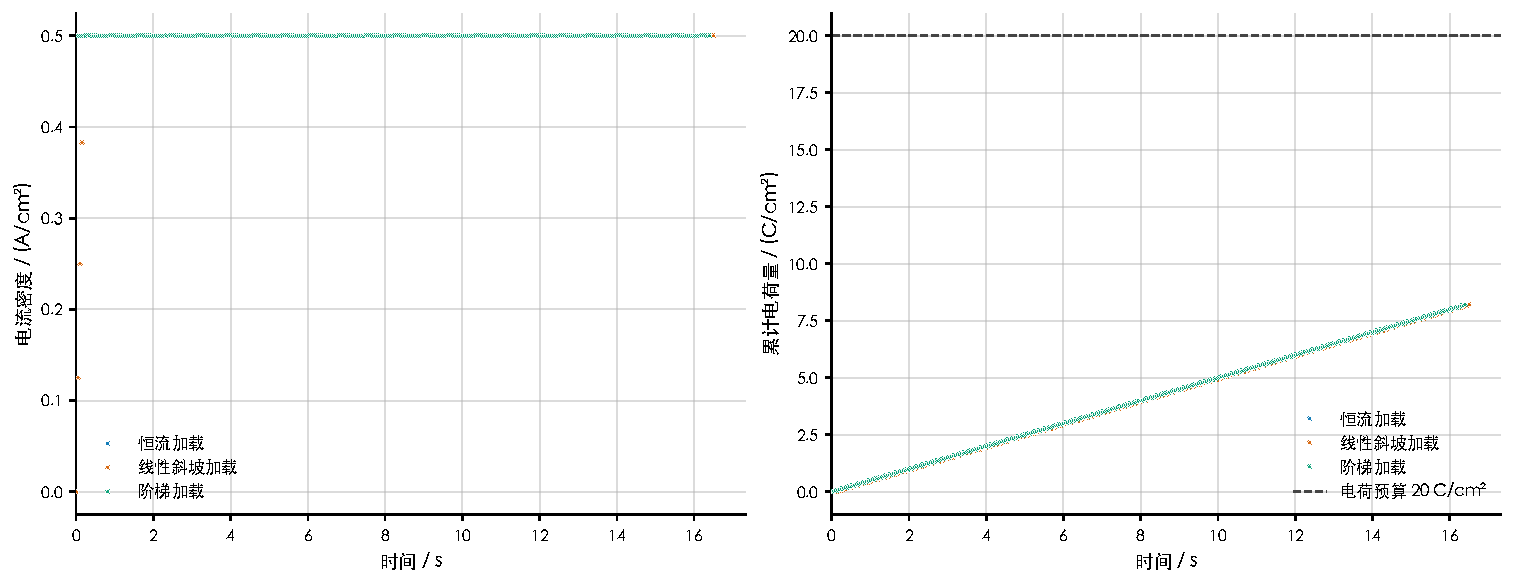
\includegraphics[width=.95\textwidth]{01_加载策略与累计电荷.pdf}
\caption{三种最优加载策略及累计电荷量随时间变化图\\恒流加载与阶梯加载数据图重合}
\label{F5-2}
\end{figure}

由表\ref{B91}和图\ref{F5-2}可以看出，在当前模型和约束条件下，恒流策略的优化结果直接达到题目允许的最大电流密度 \(0.5\,\mathrm{A\,cm^{-2}}\)，并以16.3956 s首先完成启动。三段阶梯策略经过优化后得到 \(j_1=j_2=j_3=0.5\,\mathrm{A\,cm^{-2}}\)，因此实际上退化为与恒流完全相同的控制曲线，其16.3956 s的启动时间和8.19782 \(\mathrm{C\,cm^{-2}}\) 的累计电荷量均与恒流一致。此时 \(t_1=8\) s、\(t_2=16\) s仅为三档电流相等情况下的一种等价参数表示，不具有唯一的物理切换意义。

有限搜索范围内的线性升载策略在0.2 s内由零升至 \(0.5\,\mathrm{A\,cm^{-2}}\)，启动时间为16.5021s，仅比恒流增加0.1065s，增幅约0.65\%；累计电荷量增加约0.00322 \(\mathrm{C\,cm^{-2}}\)，差异同样很小。从图5-1可以直观看出，三种策略除线性升载开始阶段存在极短的爬升过程外，随后基本均在最大允许电流下运行，因此其累计电荷曲线也高度接近。

需要特别说明线性升载策略的“最优斜率”含义。题目本身并未规定升载斜率上限，而本次有限范围搜索将达到 \(0.5\,\mathrm{A\,cm^{-2}}\) 平台的最短时间限定为0.2s，因此 \(a=2.5\,\mathrm{A\,cm^{-2}s^{-1}}\) 实际上是该有限参数域上的边界解。进一步减小平台到达时间至0.1、0.05、0.02和0.01s后，其启动时间持续逼近恒流的16.3956s。

\begin{figure}[!h]
\centering
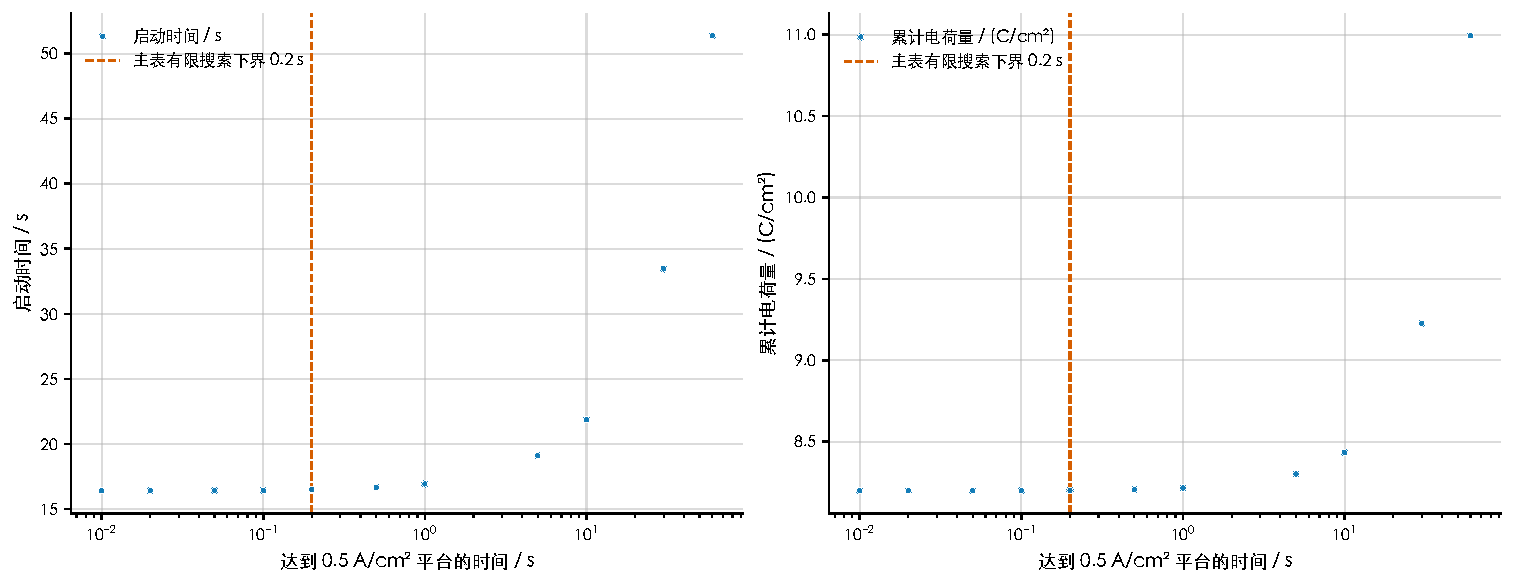
\includegraphics[width=.95\textwidth]{12_线性升载斜率极限.pdf}
\caption{线性升载平台到达时间对启动性能的影响}
\label{F5-3}
\end{figure}

由图\ref{F5-3}可见，随着平台到达时间逐渐减小，线性升载的启动时间和累计电荷量均单调趋近恒流结果。因而，在题目未额外限定电流变化速率的条件下，不应将 \(a=2.5\) 解释为线性升载策略在无限斜率范围内唯一的全局最优值；更合理的结论是：线性升载的最优性能下确界趋近于立即施加 \(0.5\,\mathrm{A\,cm^{-2}}\) 的恒流策略。
这一结果与单纯依据“先小电流抑制结冰、后大电流加速升温”的经验判断有所不同。其根本原因在于，本题 \(-10^\circ\mathrm C\) 条件下冰堵和电压约束均没有成为活跃约束。满载恒流全过程最低单片电压仍为0.497135 V，比0.30 V安全下限高约0.197 V；最大冰体积分数仅为0.019578，最大孔隙冰饱和度仅约0.0175，均远离失效边界。

因此，在当前参数范围内，减小初期电流所带来的结冰抑制收益不足以抵消产热减少造成的升温损失，优化器最终倾向于尽可能早地达到最大电流，以提高反应产热并减少端板吸热和环境散热的累计作用。

\subsubsection{电堆温度、电压与结冰状态的空间非均匀性}

三种最优策略的宏观性能十分接近，但五片单电池内部存在明显的堆叠方向温度非均匀性。图5-3给出了各片单电池及机械端板的温度演化。
\begin{figure}[!h]
\centering
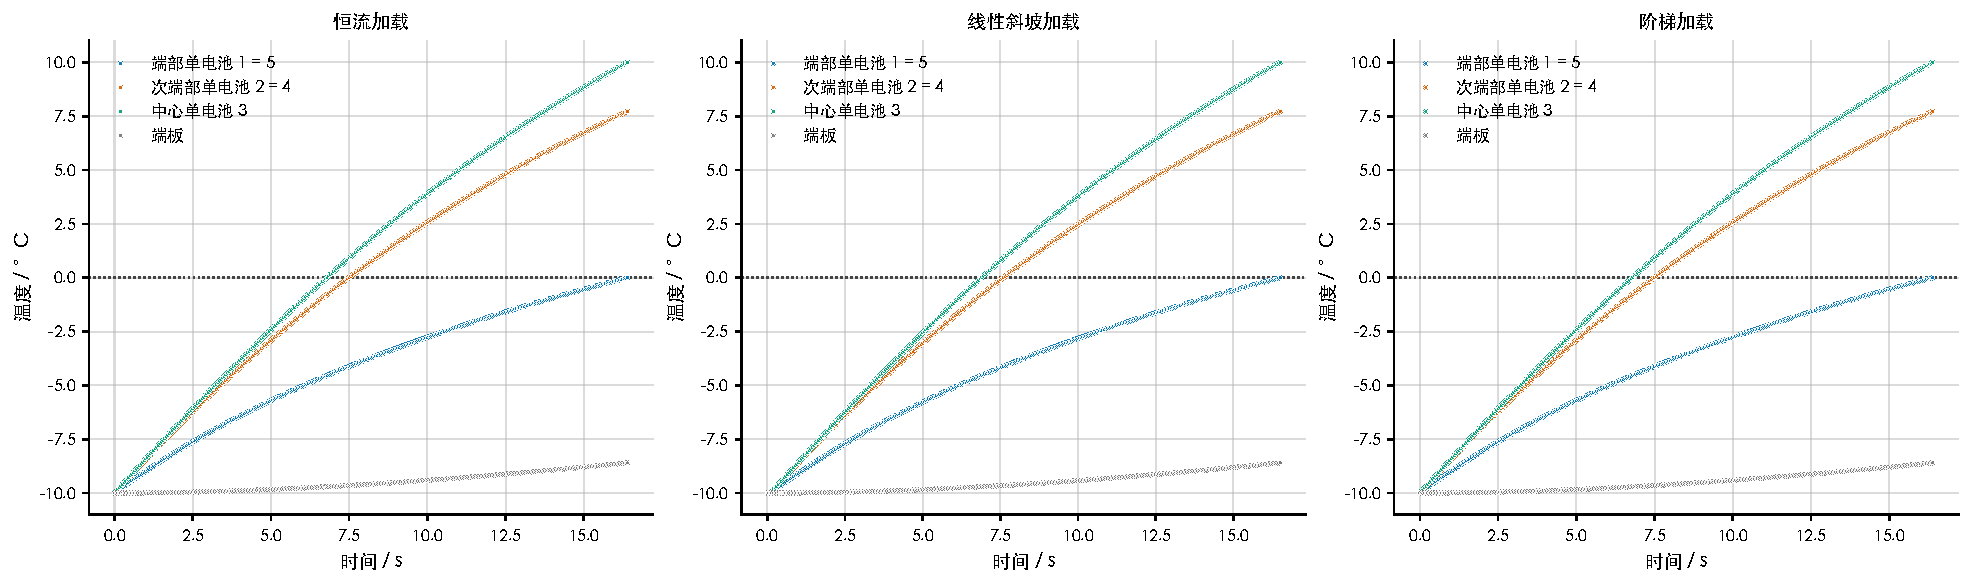
\includegraphics[width=.95\textwidth]{02_各单电池与端板温度.pdf}
\caption{三种加载策略下各单电池与端板温度随时间变化图}
\label{F5-4}
\end{figure}

由图\ref{F5-4}可见，电堆始终保持关于中心单电池3的镜面对称关系，即第1、5片温度重合，第2、4片温度重合，而中心单电池3升温最快。在最优恒流条件下，中心单电池首先越过 \(0^\circ\mathrm C\)，随后为第2、4片，而端部第1、5片最后越过冰点，因此整堆启动时刻实际上由端部单电池决定。与此同时，两块端板在启动结束时仍明显处于零下，说明冷启动期间端部单电池始终需要向大热容端板传递热量。
这一空间温差与5.2建立的热网络结构相一致。中间单电池的反应热主要用于自身升温，并可通过片间导热向外传递；而端部单电池除自身升温外，一方面需要经 \(g_E\) 向低温大热容端板供热，另一方面还承受环境对流散热，因此其有效净得热量最低。由此形成“中心片升温最快—次端部居中—端部片最慢”的稳定温度梯度。端部效应也说明，仅以电堆平均温度作为启动判据会高估实际冷启动能力，必须检查全部单电池是否同时越过冰点。



\begin{figure}[!h]
\centering
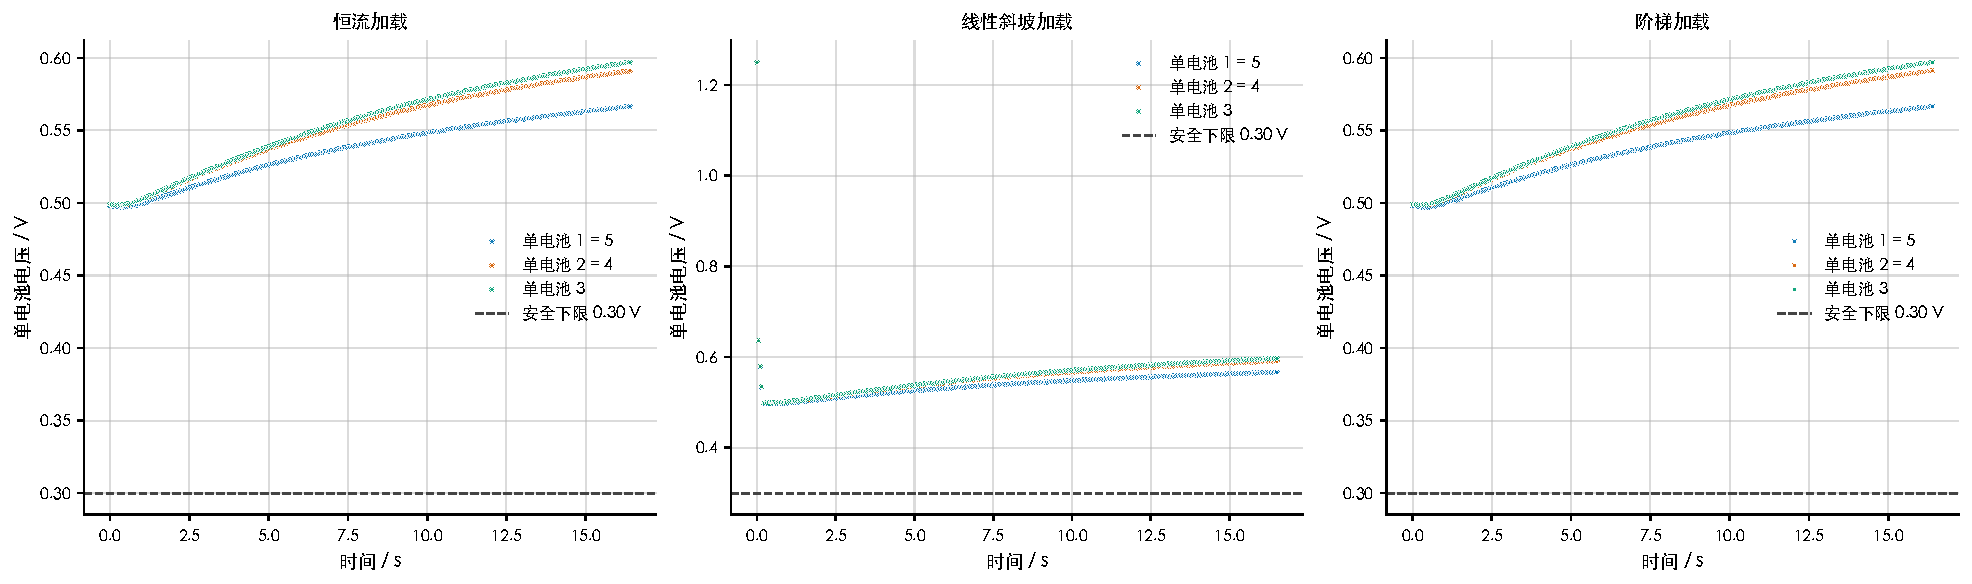
\includegraphics[width=.95\textwidth]{03_各单电池电压与安全约束.pdf}
\caption{不同加载策略下各单电池电压及安全裕度图}
\label{F5-5}
\end{figure}
温度非均匀性进一步传递至各片单电池的电化学状态。图\ref{F5-5}给出了三种最优策略下5片单电池的电压变化。
由图\ref{F5-5}可见，恒流和阶梯策略的电压轨迹几乎完全重合；线性升载因初始电流由零逐渐提高，在极短的升载阶段出现与另外两种策略不同的瞬态响应，但升至平台后同样逐渐趋于一致。5片单电池电压同样呈对称分布，其中端部第1、5片电压最低，第2、4片次之，中心第3片最高。

整个启动过程中所有单片电压均显著高于0.30 V安全下限，恒流最低值为0.497135 V，因此在 \(-10^\circ\mathrm C\) 条件下电压安全约束具有较大裕度。
随着启动进行，各片电压总体呈恢复上升趋势。这是因为温度升高后交换电流密度提高、膜质子电导增强，活化和欧姆损失逐渐下降；虽然反应产水会造成一定冰积累，但其程度不足以引起严重氧气传质受阻。因此本工况下，升温带来的电化学性能改善明显强于冰积累的不利影响。

\begin{figure}[!h]
\centering
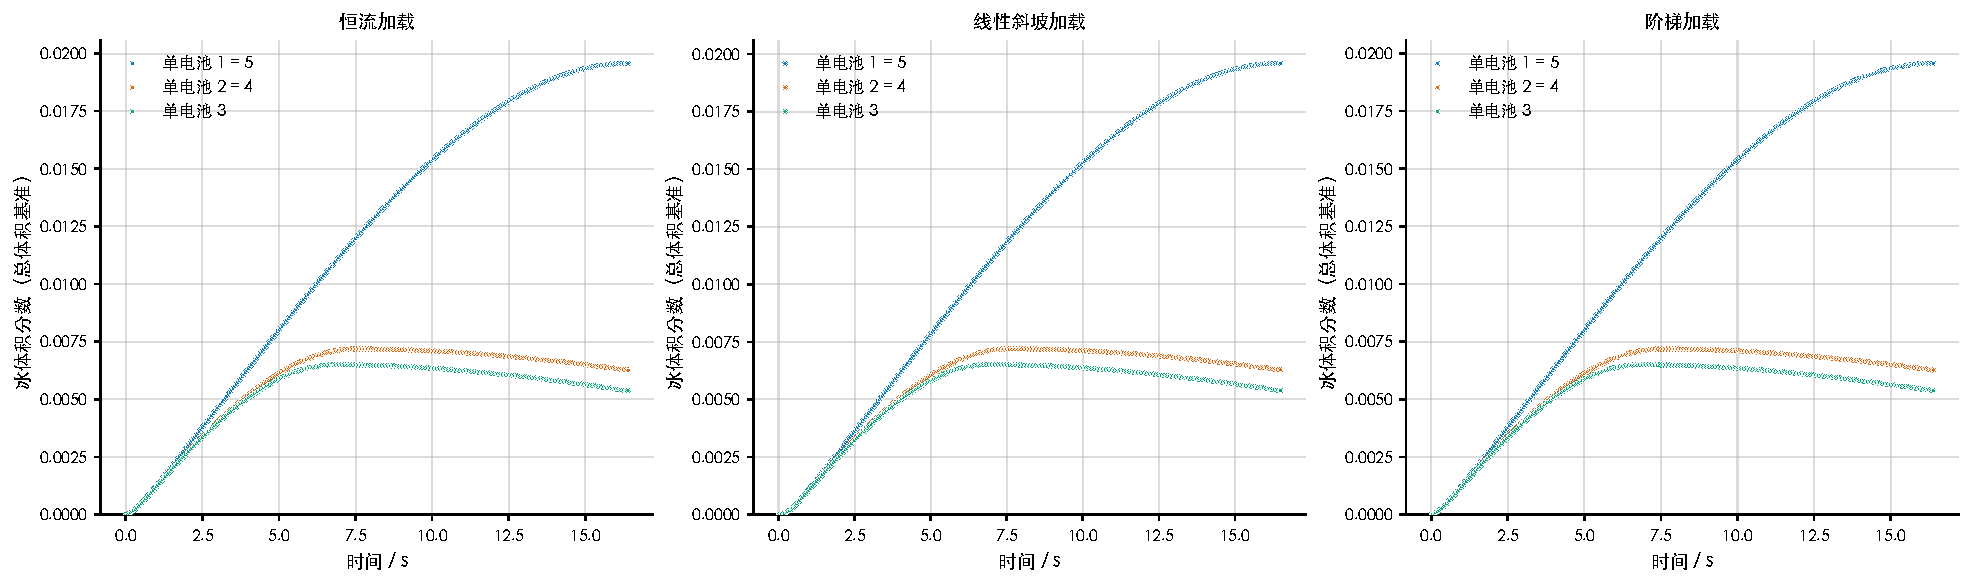
\includegraphics[width=.95\textwidth]{04_总体积基准冰体积分数.pdf}
\caption{各单电池冰积累程度图}
\label{F5-6}
\end{figure}

由图\ref{F5-6}可知，端部第1、5片冰体积分数最高，最大值约0.0196；第2、4片和中心第3片明显较低。其形成原因与温度场完全对应：端部单电池长期处于较低温度，新生成水冻结持续时间更长，而中间单电池较早升温后开始抑制继续冻结甚至出现部分融化，因此中部冰量在达到峰值后有所回落。从与实际气体传输更直接相关的孔隙冰饱和度看，端部最大值仅约0.0175，第2、4片和第3片还要更低。图中三类策略的孔隙冰轨迹同样十分接近。因此，\(-10^\circ\mathrm C\) 优化工况并不存在接近完全冰堵的情况，这进一步解释了为什么降低初始加载电流并不能换取明显的安全收益。

综合图\ref{F5-4}--图\ref{F5-6}可见，五片电堆中的首尾单电池是温度最低、冰量最大且电压最低的位置，因而是最值得关注的潜在瓶颈；但在 \(-10^\circ\mathrm C\) 工况下，其电压和冰量均仍具有较大裕度，真正决定启动时间的主要因素是端部热负荷，而非电化学失效。

\subsubsection{最低自启动初温及临界失效机理}
 在完成 \(-10^\circ\text{C}\) 三类策略优化后，进一步降低初始温度并在每个温度点重新进行策略搜索，以确定给定 \(j_{\text{max}} = 0.5 \, \text{A cm}^{-2}\) 和 \(q_{\text{max}} = 20 \, \text{C cm}^{-2}\) 条件下的最低可自启动初温。搜索首先在较大的温度区间内确定可行与不可行状态，随后在分界附近进行二分细化。

\begin{figure}[!h]
\centering
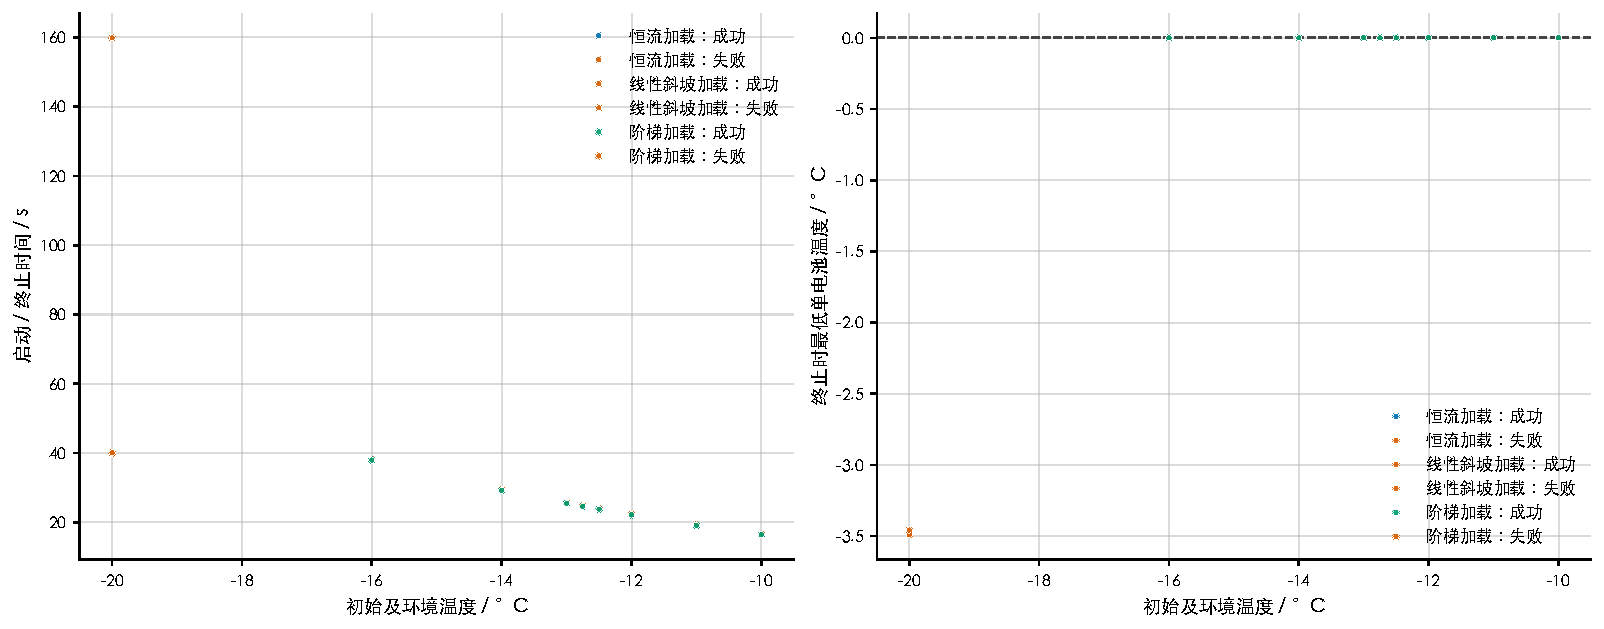
\includegraphics[width=.95\textwidth]{09_最低初温可行性搜索.pdf}
\caption{不同初始温度下电堆冷启动可行性搜索结果图}
\label{F5-7}
\end{figure}

如图\ref{F5-7}所示，随着初始温度降低，启动或终止时间总体增加，最终在约 \(-16.4^\circ\mathrm C\) 附近由成功状态转入失败状态。

三类策略的最终临界区间如表\ref{B95}所示。


\begin{table}[htbp]
    \centering
   \caption{三类加载策略的最低自启动初温搜索结果} 
    \vspace{0.3cm}
    \label{B95}
    \renewcommand{\arraystretch}{1.5} % 增加行高，匹配原图宽松排版
    \begin{tabular}{l c c}
        \toprule
        \textbf{加载策略} & \textbf{失败侧初温/\(^\circ\text{C}\)} & \textbf{成功侧初温/\(^\circ\text{C}\)} \\
        \midrule
        恒流 & -16.425781 & -16.420898 \\
        线性升载 & -16.425781 & -16.420898 \\
        三段阶梯 & -16.425781 & -16.420898 \\
        \bottomrule
    \end{tabular}
\end{table}

 三类策略的临界区间完全一致，位于
\[
(-16.425781, -16.420898]^\circ\text{C},
\]
数值上可取
\[
T_0^* \approx -16.4^\circ\text{C}.
\]

 需要强调的是，上述区间宽度仅约 \(0.0049^\circ\text{C}\)，它表示二分搜索的数值分辨率，并不意味着模型能够以 \(10^{-3} \, {}^\circ\text{C}\) 的实际物理精度预测燃料电池最低启动温度，最低自启动初温约为 \(-16.4^\circ\text{C}\)。



\begin{figure}[!h]
\centering
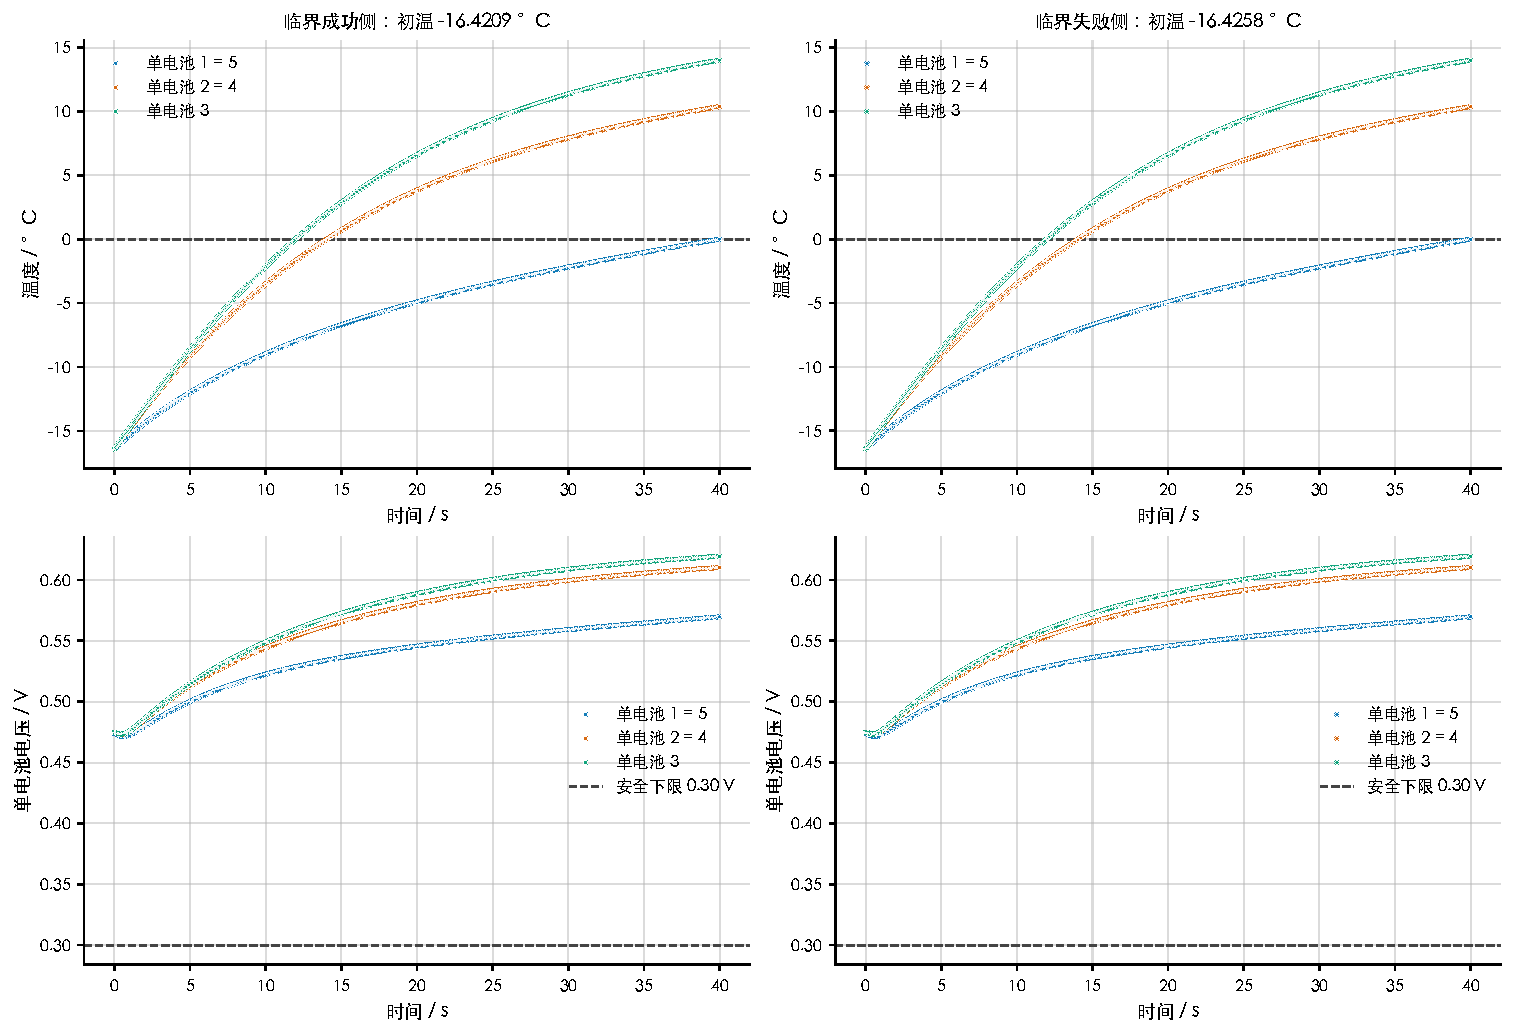
\includegraphics[width=.95\textwidth]{07_最低启动温度两侧轨迹.pdf}
\caption{临界初温两侧各单电池温度与电压演化图}
\label{F5-8}
\end{figure}
为了确定临界温度以下的直接失效原因，图\ref{F5-8}比较了临界成功侧和失败侧的温度与电压轨迹。
从图\ref{F5-8}可以看到，无论临界成功侧还是失败侧，中心单电池3均较早越过冰点，第2、4片随后越过，而第1、5片始终升温最慢。

 当 \(T_0 = -16.420898^\circ\text{C}\) 时，端部单电池能够在电荷预算耗尽前刚好越过 \(0^\circ\text{C}\)，电堆实现启动；而当初温仅降低至 \(-16.425781^\circ\text{C}\) 时，累计电荷已经达到 \(20.000000 \, \text{C cm}^{-2}\)，端部最低温度仍为 \(-0.001425^\circ\text{C}\)，因此无法满足全部单电池同时高于冰点的启动条件。此时全过程最低电压仍为 \(0.471291 \, \text{V}\)，远高于 \(0.30 \, \text{V}\) 安全下限。

 由此可以明确判断：本模型下最低自启动初温附近首先触发的并不是电压崩溃或严重冰堵，而是累计电荷预算耗尽；第1、5片端部单电池由于仍未越过冰点而成为整堆启动失败的关键单电池。

 为使这一失效机理更加清楚，可以进一步考察更低的 \(-18^\circ\text{C}\) 工况。在最大恒流 \(0.5 \, \text{A cm}^{-2}\) 下运行 40 s 后，累计电荷恰好耗尽 \(20 \, \text{C cm}^{-2}\)。此时端部第1、5片温度仍仅为 \(-1.5527^\circ\text{C}\)，而中心第3片已经升至 \(12.4066^\circ\text{C}\)，二者温差达到约 \(14^\circ\text{C}\)；全过程最低电压仍为 \(0.464365 \, \text{V}\)，最大孔隙冰饱和度仅 \(0.099345\)，同样未触及电压或冰堵约束。

 该结果揭示出低温电堆冷启动具有明显的“内部过热—端部欠热”特征：中心区域已经获得了远超越冰点所需的热量，而端部单电池仍在持续向低温端板传热并承担环境散热，最终导致有限电荷量不能被有效地全部用于抬升瓶颈单电池温度。因此进一步降低初温后，制约整堆自启动能力的核心并非总产热绝对不足，而是热量沿堆叠方向分配不均以及端部额外热负荷造成的局部能量不足。

\begin{figure}[!h]
\centering
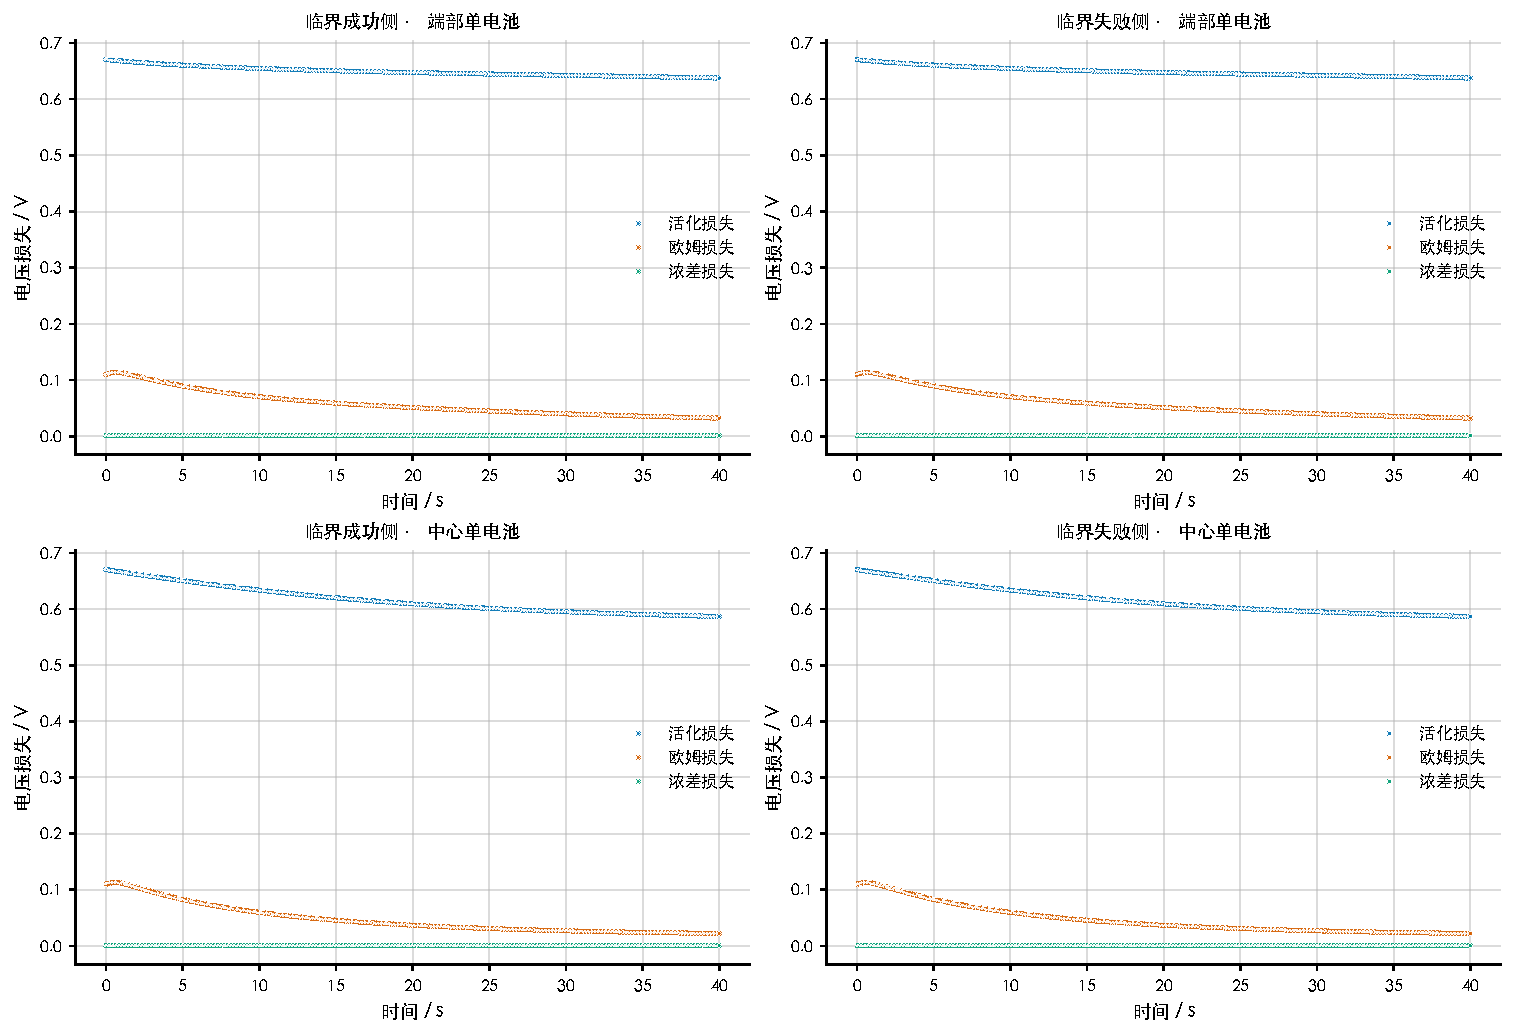
\includegraphics[width=.95\textwidth]{08_临界启动电压损失分解.pdf}
\caption{临界启动工况端部与中心单电池电压损失分解图}
\label{F5-9}
\end{figure}

进一步利用电压损失分解可以检验是否存在潜在的冰堵失压机制。由图\ref{F5-9}可见，无论在临界成功侧还是失败侧，电压损失始终以活化损失为主，欧姆损失次之，浓差损失最小；端部单电池的各项损失总体高于中心单电池，但并未出现浓差极化突增所对应的传质崩溃特征。以 \(-18^\circ\mathrm C\) 终止状态为例，端部单电池活化、欧姆和浓差损失分别为0.646002、0.035676和0.001253 V，而中心单电池分别为0.592058、0.022743和0.000127 V。端部浓差损失虽然约为中心片的一个数量级，但绝对值仍只有毫伏量级，并不足以造成电压跌破0.30 V。这说明随着初温降低，冰量增加和低温极化确实恶化了端部电化学性能，但在当前电流与电荷约束下，它们仍是次要效应，尚未先于热量约束触发失效。

因此，最低温度附近的主导失效链条可以概括为：
初始温度降低 → 跨越冰点所需显热增加，同时端板保持更低温度 → 端部单电池向端板供热及环境散热增加 → 端部温升显著落后于中部 → 累计电荷达到20 \(\mathrm{C\,cm^{-2}}\) 时端部仍未越过0 ℃ → 整堆启动失败。
该机理同时解释了为什么临界低温下第1、5片始终是关键单电池，也说明若希望进一步拓展电堆的自冷启动温度范围，相比单纯调整电流加载曲线，降低端板热负荷、改善端部保温或引入针对端部的辅助加热可能更为有效。

\subsubsection{数值收敛性与结果稳健性分析}
为保证上述策略比较和最低初温判断并非由离散参数造成，进一步对时间步和空间网格进行了加密计算。正式结果采用每片232个输运网格和
\(\Delta t=0.003125\,\mathrm s\)；进一步加密至464个网格、\(\Delta t=0.0015625\,\mathrm s\) 后，恒流最优方案的启动时间仅变化0.001473 s，而最大冰体积分数变化约1.070\%。

\begin{figure}[!h]
\centering
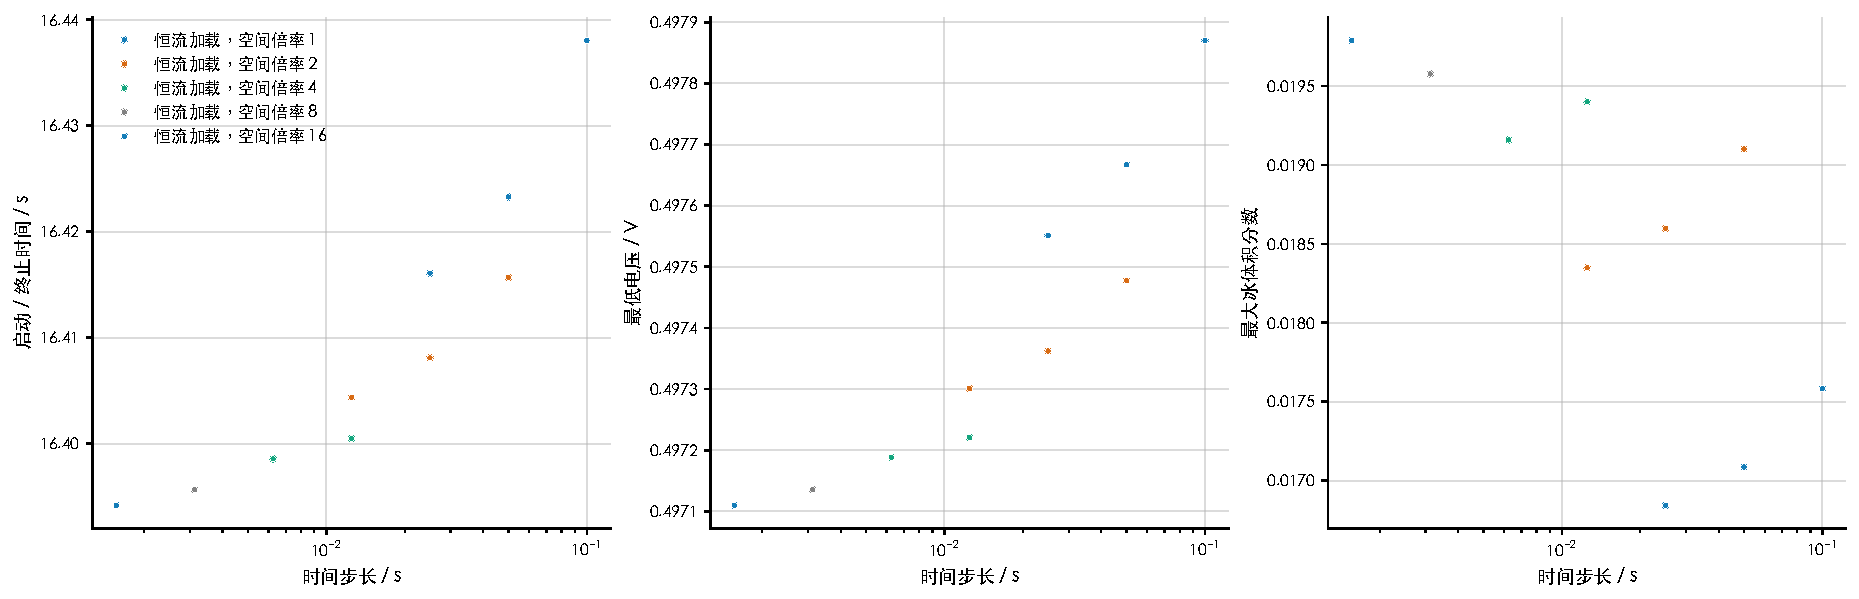
\includegraphics[width=.95\textwidth]{10_时间空间离散收敛性.pdf}
\caption{时间—空间离散加密下主要输出量的收敛性图}
\label{F5-10}
\end{figure}

由图\ref{F5-10}可见，随着时间步减小和空间网格加密，启动时间与最低电压均逐渐趋于稳定，其中启动时间的离散敏感性很小；相比之下，最大冰体积分数对离散精度更加敏感。因此，本文关于启动时间、最优策略和最低初温的宏观结论具有较好的数值稳定性。


综合上述结果，问题二的两个核心结论可以统一概括为：在 \(-10^\circ\mathrm C\) 条件下，冰堵和最低电压约束均具有较大裕度，提高初始电流的产热收益占据主导，因此最短启动对应于尽早施加
\(0.5\,\mathrm{A\,cm^{-2}}\) 的满载控制，恒流与退化后的三段阶梯均在约16.40 s内完成启动，而无斜率上限时线性升载的性能下确界同样趋近该结果；在
\(20\,\mathrm{C\,cm^{-2}}\)
累计电荷约束下，五片电堆最低可自冷启动初温约为
\(-16.4^\circ\mathrm C\)，低于该温度后首先失效的是第1、5片端部单电池，其直接原因是端板吸热和环境散热使端部温升严重滞后，导致电荷预算耗尽时仍未越过冰点。

\subsection{问题二小结}
针对有限电流密度和累计电荷量约束下五片燃料电池电堆的自冷启动问题，本文在问题一单电池水—冰—热—电耦合模型基础上，进一步引入相邻单电池间导热、共享双极板热容量分配、端板热惯性及端部环境散热，建立了由5个单电池节点和2个端板节点组成的电堆瞬态热网络，实现了堆叠方向传热与各片水冰状态、电压响应之间的双向耦合。在此基础上，采用控制向量参数化方法描述恒流、线性升载和三段阶梯三类加载策略，并通过“内层瞬态仿真—外层参数优化”确定不同策略下的最短启动时间。

在初始温度为 \(-10^\circ\mathrm C\) 时，恒流策略的最优电流密度达到允许上限 \(0.5\,\mathrm{A\,cm^{-2}}\)，电堆在16.3956 s完成启动，累计消耗电荷量为8.19782 \(\mathrm{C\,cm^{-2}}\)；三段阶梯策略优化后退化为相同的满载恒流形式，得到完全一致的启动结果。有限搜索范围内线性升载的启动时间为16.5021 s，而随着升载时间进一步缩短，其性能持续趋近恒流结果。该结果表明，在本题 \(-10^\circ\mathrm C\) 工况下，最低单片电压和冰量约束均具有较大安全裕度，减小初期电流所获得的结冰抑制作用不足以抵消产热下降，因此尽早达到最大允许电流更有利于缩短启动时间。

进一步分析五片单电池的状态演化发现，电堆存在明显的轴向热非均匀性：中心第3片升温最快，第2、4片次之，而第1、5片端部单电池升温最慢，同时表现出较低的电压和较高的冰积累。其根本原因在于端部单电池除自身升温外，还需向大热容端板供热并承担环境散热，使端部有效净得热量低于中部。因此，在当前参数范围内，整堆启动时刻主要由两端单电池能否越过冰点决定，而不是由严重冰堵或电压安全约束决定。
在 \(j_{\max}=0.5\,\mathrm{A\,cm^{-2}}\)、\(q_{\max}=20\,\mathrm{C\,cm^{-2}}\) 的约束下，通过逐级降温与二分搜索得到电堆最低可自冷启动初温约为 \(-16.4^\circ\mathrm C\)。临界失败侧在累计电荷量耗尽时，第1、5片端部单电池仍未升至 \(0^\circ\mathrm C\)，而最低电压仍明显高于0.30 V，冰堵程度亦未达到失效阈值，因此临界低温下的直接失效机制属于端部局部能量不足导致的电荷预算耗尽，而非电压崩溃或孔隙完全冰堵。

同时，时间—空间加密结果表明启动时间对离散参数已基本收敛，说明最优策略及临界初温等宏观结论具有较好的数值稳定性。由此可见，若需进一步拓展更低温度下的启动能力，仅依靠调整自启动电流的改善空间有限，后续应重点针对端部热负荷和温度非均匀性引入辅助加热措施，这也为问题三的电堆辅助冷启动优化提供了直接依据。

\section{问题三的分析与求解}
\subsection{问题描述和分析}

问题三要求在问题二五片电堆瞬态自冷启动模型的基础上，进一步考虑极低温环境下反应产热不足的问题，在各片单电池双极板内引入功率可独立调节的电热丝，建立电堆辅助冷启动模型。初始及环境温度降至 \(-30^\circ\mathrm C\) 后，电堆需要克服更大的升温需求，同时端部单电池还受到端板吸热和环境散热的共同作用，仅依靠电化学反应产热难以在有限电荷量内使五片单电池均越过冰点。因此，需要通过外部辅助热源弥补冷启动过程中的热量缺口。

根据辅助加热与电流加载的先后关系，本问分别研究纯预加热启动和恒定功率协同启动两种策略。纯预加热策略在加载电流前先利用电热丝提高电堆温度，可避免低温产水引起的大量结冰，但其升温所需热量主要由辅助加热承担；恒定功率协同策略则从启动初期同时施加电流和辅助加热，使电化学反应热与电热丝共同推动升温，但在电池越过冰点之前仍存在“产水—冻结—升温”的竞争过程。因此，两种策略在辅助能耗、启动过程和冰堵抑制能力之间具有不同的权衡关系。

基于上述特点，本文沿用问题二建立的五片电堆热网络以及各片单电池的水—冰—热—电耦合模型，在各电池节点能量方程中增加独立可控的辅助加热项，并建立相应的分片能耗计量模型。在满足单片温度、电压、冰体积分数及累计电荷量等启动约束的条件下，以各片加热功率密度和加热持续时间为决策变量，以辅助加热总能耗最小为目标，分别求解两种冷启动策略，并进一步比较其总能耗、启动时间、各片能耗分配及端部单电池的结冰特征，从而确定极低温条件下合理的辅助冷启动方式。

\subsection{五片电堆辅助冷启动模型的建立}

问题二已经建立了由 5 个单电池节点和 2 个端板节点构成的电堆瞬态热网络，并实现了片间导热、端板热惯性与各片水—冰—热—电状态之间的耦合。问题三在此基础上不改变各片单电池内部的三相水迁移、冰占孔、气体传输及电压计算关系，而是在各片双极板内增加可独立调节的电热丝，将辅助加热作为新的可控热源并入电堆能量方程。由此，冷启动过程的热量来源由单一的电化学反应产热扩展为“反应产热—辅助加热”共同供热，并进一步建立与之对应的辅助能耗计量和两类启动时序模型。
\subsubsection{电热丝布置、功率约束及基本假设}
题目规定在各片单电池的双极板内分别设置功率可独立调节的电热丝。考虑双极板具有较高导热系数，本文将电热丝视为沿双极板平面均匀铺设的薄面热源，其覆盖范围与单电池活化面积一致，忽略加热元件自身厚度和热容以及面内温度梯度。五片单电池分别配置一组独立加热单元，各加热单元只通过对应电池节点向电堆热网络输入能量。该处理与第五章采用的共享双极板热容分配方式保持一致。

 第 \(k\) 片电热丝的有效加热面积等于单电池截面积，即
\begin{equation}
A_k = A = 25 \, \text{cm}^2 = 2.5 \times 10^{-3} \, \text{m}^2, \qquad k = 1, \dots, 5. \tag{6-1}
\end{equation}

 记第 \(k\) 片电热丝的加热功率密度为 \(q_k\)，则其总加热功率以及题目给定的功率约束分别为
\begin{equation}
P_k = A_k q_k, \qquad 0 \leq q_k \leq 1 \, \text{W cm}^{-2}, \qquad k = 1, \dots, 5. \tag{6-2}
\end{equation}

 因此，单片电热丝最大加热功率为 25 W，五片同时满功率工作时总装机功率上限为 125 W。

 在问题一、问题二模型假设的基础上，本问进一步认为：电热丝为理想电阻加热元件，输入电能全部转化为热能；加热期间各片功率密度保持恒定，但五片之间允许取不同值；辅助加热不直接改变水迁移、电化学反应及相变模型，而是通过提高单片温度间接改变结冰和电压状态；两块端板不设置独立电热丝，仅通过与端部单电池之间的导热获得热量。电堆所有部件与环境初始温度统一取
\begin{equation}
T_k(0) = T_{\text{EL}}(0) = T_{\text{ER}}(0) = T_{\text{amb}} = 243.15 \, \text{K} = -30^\circ\text{C}. \tag{6-3}
\end{equation}

 同时沿用前两问的吹扫初始条件，孔隙液态水和冰初值取零，质子交换膜初始含水量取 \(\lambda_0 = 3\)。

\subsubsection{辅助加热源项及电堆能量方程}

 设电热丝嵌置于对应单电池的双极板内部。为与问题一的分布参数能量方程统一，将第 \(k\) 片电热丝的面功率密度折算为双极板内部的等效体积热源。若以双极板厚度 \(L_{\text{BP}}\) 为等效发热厚度，则有
\begin{equation}
\dot{q}_{\text{aux}}(x,t) = \begin{cases}
\frac{q_k^{(\text{SI})}}{L_{\text{BP}}}, & x \text{ 位于第 } k \text{ 片加热区域且电热丝接通}, \\
0, & \text{其他区域},
\end{cases} \qquad q_k^{(\text{SI})} = 10^4 q_k. \tag{6-4}
\end{equation}

 其中 \(q_k^{(\text{SI})}\) 的单位为 \(\text{W m}^{-2}\)。由此，问题一的局部能量守恒方程可扩展为
\begin{equation}
(\rho c_p)_{\text{eff}} \frac{\partial T}{\partial t} = \frac{\partial}{\partial x} \left( k_{\text{eff}} \frac{\partial T}{\partial x} \right) + \dot{q}_{\text{gen}} + \dot{q}_{\text{pc}} + \dot{q}_{\text{ads}} + \dot{q}_{\text{aux}}. \tag{6-5}
\end{equation}

 辅助热源只作用于双极板加热区域，非加热区域仍仅进行储热和导热，不产生电化学反应或水相变。由于式（6-4）中的等效厚度在体积积分后消去，因此其具体取值只影响热源在分布模型中的空间定位，不改变进入电池节点的总辅助热量。

 进一步将辅助体积热源在第 \(k\) 片电池的加热区域内积分，并除以活化面积 \(A\)，可得进入节点热网络的辅助加热面功率
\begin{equation}
\bar{q}_{\text{aux},k} = \frac{1}{A} \int_{\Omega_{\text{aux},k}} \dot{q}_{\text{aux}} \, \mathrm{d}V = q_k^{(\text{SI})} \frac{A_k}{A} = 10^4 q_k, \qquad k = 1, \dots, 5. \tag{6-6}
\end{equation}

 因此，辅助加热可直接作为一个非负外部热源加入第五章建立的五片电堆热网络。记第 \(k\) 片单电池原有单位面积内源为
\begin{equation}
\bar{q}_k = j (E_{\text{th}} - V_k) + \bar{q}_{\text{pc},k}, \tag{6-7}
\end{equation}

 其中第一项为电化学反应产热，第二项综合表示该片内部水相变等过程引起的热效应。加入电热丝后，七节点热网络写为
\begin{equation}
\left\{
\begin{aligned}
& C_{A,1} \frac{\text{d}T_1}{\text{d}t} = \bar{q}_1 + \bar{q}_{\text{aux},1} + g_c(T_2 - T_1) + g_E(T_{\text{EL}} - T_1) - h(T_1 - T_{\text{amb}}), \\
& C_{A,k} \frac{\text{d}T_k}{\text{d}t} = \bar{q}_k + \bar{q}_{\text{aux},k} + g_c(T_{k-1} - T_k) + g_c(T_{k+1} - T_k), \quad k = 2, 3, 4, \\
& C_{A,5} \frac{\text{d}T_5}{\text{d}t} = \bar{q}_5 + \bar{q}_{\text{aux},5} + g_c(T_4 - T_5) + g_E(T_{\text{ER}} - T_5) - h(T_5 - T_{\text{amb}}), \\
& C_{A,\text{EP}} \frac{\text{d}T_{\text{EL}}}{\text{d}t} = g_E(T_1 - T_{\text{EL}}), \\
& C_{A,\text{EP}} \frac{\text{d}T_{\text{ER}}}{\text{d}t} = g_E(T_5 - T_{\text{ER}}).
\end{aligned}
\right.
\tag{6-8}
\end{equation}

 式中，\(g_c\) 为相邻单电池之间的等效导热系数，\(g_E\) 为端部单电池与端板之间的等效导热系数，\(h\) 为端部环境对流换热系数，其取值均沿用问题二。各节点面热容同样保持第五章的计算方式，其中端部电池干燥参考面热容约为 \(4600.27 \, \text{J m}^{-2}\text{K}^{-1}\)，中间三片约为 \(3083.59 \, \text{J m}^{-2}\text{K}^{-1}\)，单块端板面热容为 \(39500 \, \text{J m}^{-2}\text{K}^{-1}\)。单电池 MEA 部分的等效热容仍随局部水冰状态逐时刻更新。

 定义电堆温度状态向量
\begin{equation}
\boldsymbol{\theta} = [T_{\text{EL}}, T_1, T_2, T_3, T_4, T_5, T_{\text{ER}}]^{\text{T}}, \tag{6-9}
\end{equation}

 则式（6-8）可以写成紧凑矩阵形式
\begin{equation}
\mathbf{C} \frac{\text{d}\boldsymbol{\theta}}{\text{d}t} = -\mathbf{G}\boldsymbol{\theta} + \mathbf{b} + \mathbf{b}_{\text{aux}}, \tag{6-10}
\end{equation}

 其中新增的辅助加热源向量为
\begin{equation}
\mathbf{b}_{\text{aux}} = [0, \bar{q}_{\text{aux},1}, \bar{q}_{\text{aux},2}, \bar{q}_{\text{aux},3}, \bar{q}_{\text{aux},4}, \bar{q}_{\text{aux},5}, 0]^{\text{T}}. \tag{6-11}
\end{equation}

 可见，引入电热丝后热网络的拓扑、电导矩阵和热容量矩阵均保持不变，仅源向量中增加五个独立可控的辅助热源，因此问题三能够直接继承问题二已经建立的瞬态求解框架。


 将（6-8）中的七个节点方程求和，片间导热项 \(g_c\) 与电池—端板导热项 \(g_E\) 均在系统内部成对抵消，可得整个电堆的瞬时能量平衡
\begin{equation}
\sum_{k=1}^5 C_{A,k} \frac{\text{d}T_k}{\text{d}t} + C_{A,\text{EP}} \left( \frac{\text{d}T_{\text{EL}}}{\text{d}t} + \frac{\text{d}T_{\text{ER}}}{\text{d}t} \right) = \sum_{k=1}^5 \bar{q}_k + \sum_{k=1}^5 \bar{q}_{\text{aux},k} - h(T_1 - T_{\text{amb}}) - h(T_5 - T_{\text{amb}}). \tag{6-12}
\end{equation}

 式（6-12）说明，片间导热和端板耦合只负责热量在电堆内部重新分配，真正改变系统总能量的是电化学及相变内源、辅助加热和端部环境散热，因此该式也可作为后续数值计算中热量守恒检验的依据。

 需要进一步说明将电热丝功率直接并入单电池节点的合理性。双极板厚度仅为 2 mm，导热系数为 \(95 \, \text{W m}^{-1}\text{K}^{-1}\)，其沿厚度方向热阻为
\begin{equation}
R_{\text{BP}} = \frac{L_{\text{BP}}}{k_{\text{BP}}} = \frac{0.002}{95} = 2.11 \times 10^{-5} \, \text{m}^2\text{K W}^{-1}. \tag{6-13}
\end{equation}

 该值仅约为单片 MEA 贯穿热阻的 0.74\%，说明在本题几十秒量级的辅助启动过程中，双极板内部温差相对于电池整体温差较小。同时，问题二已将共享双极板的热容量分摊到相邻电池节点，因此不再为电热丝或双极板单独增加温度自由度，而将其功率直接加入所属电池节点，在集中参数模型下具有一致性。

\subsubsection{辅助加热能耗与启动成功判据}

 辅助启动策略的优化目标是减小外部电加热所消耗的能量。根据题目定义，第 \(k\) 片电热丝在实际接通区间内的耗能以及全堆辅助总能耗分别为
\begin{equation}
E_k = A_k \int q_k(t) \, \text{d}t, \qquad E_{\text{aux}} = \sum_{k=1}^5 E_k = \sum_{k=1}^5 A_k \int q_k(t) \, \text{d}t. \tag{6-14}
\end{equation}

 本问两类策略均采用“接通期间功率恒定”的形式。若各片共同加热持续时间记为 \(t_\bullet\)，其中纯预加热策略取 \(t_\bullet = t_{\text{pre}}\)，恒定功率协同策略取 \(t_\bullet = t_h\)，则有
\begin{equation}
E_k = A q_k t_\bullet = 25 q_k t_\bullet, \qquad E_{\text{aux}} = 25 t_\bullet \sum_{k=1}^5 q_k. \tag{6-15}
\end{equation}

 式中 \(q_k\) 以 \(\text{W cm}^{-2}\) 计，\(t_\bullet\) 以 \(\text{s}\) 计，则 \(E_k\) 的单位为 \(\text{J}\)。该能耗表达式与式（6-6）中的节点辅助热源严格一致，可在数值计算中通过热网络积分进行交叉校验。

 两种策略在进入电流加载阶段后均采用题目规定的统一加载曲线。为避免纯预加热阶段与实际加载时间混淆，记 \(\xi\) 为“自电流开始加载后经过的时间”，则
\begin{equation}
j_L(\xi) = \begin{cases}
0.005\xi, & 0 \leq \xi \leq 60 \, \text{s}, \\
0.3, & \xi > 60 \, \text{s},
\end{cases} \qquad [\text{A cm}^{-2}]. \tag{6-16}
\end{equation}

 相应的单位面积累计电荷量为
\begin{equation}
Q_L(\xi) = \int_0^\xi j_L(\tau) \, \text{d}\tau = \begin{cases}
0.0025\xi^2, & 0 \leq \xi \leq 60 \, \text{s}, \\
9 + 0.3(\xi - 60), & \xi > 60 \, \text{s}.
\end{cases} \tag{6-17}
\end{equation}

 由于累计电荷上限仍为 \(20 \, \text{C cm}^{-2}\)，故加载阶段允许的最长持续时间为
\begin{equation}
\xi_{Q_{\text{max}}} = 60 + \frac{20 - 9}{0.3} = 96.67 \, \text{s}. \tag{6-18}
\end{equation}


 因此，无论采用何种辅助加热方式，若从实际开始加载电流起经过约 96.67 s 后仍未达到成功状态，则认为在给定电荷预算下启动失败。

 问题三继续沿用问题二的启动成功判据。设 \(t_s\) 为从整个辅助启动过程开始计时的成功时刻，则五片单电池必须同时满足温度和冰量终端条件，并在整个启动过程中满足单片电压安全约束，同时累计电荷量不得超过给定上限，即
\begin{equation}
\left\{
\begin{aligned}
& \min_{1 \leq k \leq 5} T_k(t_s) > 0^\circ\text{C}, \\
& \max_{1 \leq k \leq 5} \varepsilon_{\text{ice},k}(t_s) < 0.99, \\
& \min_{0 \leq t \leq t_s} \min_{1 \leq k \leq 5} V_k(t) \geq 0.30 \, \text{V}, \\
& \int_0^{t_s} j(t) \, \text{d}t \leq 20 \, \text{C cm}^{-2}.
\end{aligned}
\right.
\tag{6-19}
\end{equation}

 其中温度判据仅针对 5 片单电池，左右端板属于热网络边界节点，不作为启动成功的温度判定对象；电压则属于全过程路径约束，只要任一单电池在此前时刻跌破 0.30 V，即判定该方案不可行。该定义与第五章的启动成功口径保持一致。

\subsubsection{两类辅助冷启动策略的混合动力学模型}

 辅助加热功率与电流加载在时间轴上的组合方式决定了不同的冷启动策略。本问分别研究纯预加热启动和恒定功率协同启动。两者均可描述为输入在特定时刻发生切换、而温度、水冰状态及气体状态连续演化的混合动态系统。

 对于纯预加热策略 P，首先在无外部电流条件下利用电热丝升高电堆温度，在预热时间 \(t_{\text{pre}}\) 后关闭电热丝并开始加载题给电流。其输入可表示为
\begin{equation}
\left\{
\begin{aligned}
j_P(t) &= 0, \qquad & \bar{q}_{\text{aux},k}^P(t) &= 10^4 q_k, \qquad & 0 &\leq t < t_{\text{pre}}, \\
j_P(t) &= j_L(t - t_{\text{pre}}), \qquad & \bar{q}_{\text{aux},k}^P(t) &= 0, \qquad & t &\geq t_{\text{pre}}.
\end{aligned}
\right.
\tag{6-20}
\end{equation}

 因此，预热阶段不存在电化学反应产热和反应产水，升温主要由电热丝输入完成；进入加载阶段后，辅助热源关闭，系统在预热所得温度场基础上按照问题一、问题二建立的水—冰—热—电耦合模型继续演化。为了保证预热阶段完成基本越冰要求，切换时刻需满足
\begin{equation}
\min_{1 \leq k \leq 5} T_k(t_{\text{pre}}) > 0^\circ\text{C}. \tag{6-21}
\end{equation}

 需要指出的是，式（6-21）只是预热切换的基本可行条件，\(t_{\text{pre}}\) 本身仍作为后续优化中的决策变量，因此模型并不要求电热丝必须在“首次越过冰点”的瞬间关闭；若继续加热能够形成必要的热裕量，也允许取更大的预热时间。

 对于恒定功率协同策略 C，从 \(t = 0\) 起同时加载电流并开启电热丝，使反应热和辅助热共同驱动升温；加热持续至时刻 \(t_h\) 后关闭，而电流加载继续按照既定曲线进行，其输入写为
\begin{equation}
\left\{
\begin{aligned}
j_C(t) &= j_L(t), \qquad & \bar{q}_{\text{aux},k}^C(t) &= 10^4 q_k, \qquad & 0 &\leq t < t_h, \\
j_C(t) &= j_L(t), \qquad & \bar{q}_{\text{aux},k}^C(t) &= 0, \qquad & t &\geq t_h.
\end{aligned}
\right.
\tag{6-22}
\end{equation}

 与纯预加热不同，协同策略在低温升温阶段已经产生反应水，因此早期同时存在反应产水、冻结、冰占孔和辅助升温过程。电热丝一方面直接提高温度，另一方面通过缩短电池处于零下温区的时间间接抑制冰累积。这里将 \(t_h\) 与电堆满足启动条件的时刻 \(t_s\) 分别处理，模型不预先假定 \(t_h = t_s\)；二者之间的关系由后续能耗优化结果决定。

 为统一描述两种策略的温度过零状态，定义
\begin{equation}
s_T(t) = \min_{1 \leq k \leq 5} T_k(t). \tag{6-23}
\end{equation}

 当 \(s_T(t)\) 由负值变为正值时，表示五片单电池首次共同越过冰点。除该状态事件外，模型还包含电热丝关闭事件 \(t = t_{\text{pre}}\) 或 \(t = t_h\)，以及电流在 60 s 处由线性升载转入恒流平台的输入切换事件。所有切换时刻仅改变外部输入 \(j(t)\) 和 \(\bar{q}_{\text{aux},k}(t)\)，各片温度、端板温度、水冰质量及气体浓度均保持连续，从而保证切换前后的质量和能量计量一致。

 此外，在纯预加热初期，启动前已完成吹扫，孔隙液水和冰初值均为零；膜初始含水量又与非冻结膜水阈值相同，即 \(\lambda_0 = \lambda_{\text{nf}} = 3\)，因此初始可冻结膜水满足
\begin{equation}
m_{\text{free}}(0) = [m_l(0) - W_\lambda \lambda_{\text{nf}}]_+ = W_\lambda [\lambda_0 - \lambda_{\text{nf}}]_+ = 0. \tag{6-24}
\end{equation}

 这说明预热阶段在理论上主要表现为显热升温过程，不存在由初始自由水大量冻结造成的额外热负荷。不过，为保持与问题一完整水相模型的一致性，正式数值求解中仍保留膜—催化层水交换以及相变热源，不人为将 \(\bar{q}_{\text{pc},k}\) 或冰量强制设为零，因此后续结果中对纯预加热策略采用“冰量接近于零”而非严格为零的表述。

 至此，问题二的五片电堆瞬态模型已扩展为含五路独立辅助热源的电堆辅助冷启动模型。模型以 \((q_1, q_2, q_3, q_4, q_5)\) 及加热持续时间为外部控制量，在统一电流加载协议下同步计算各片温度、电压、水冰状态和辅助能耗，并通过式（6-19）判断方案是否满足冷启动要求，为下一节两类辅助加热策略的能耗最小优化与数值求解提供统一的状态模型。

\subsection{辅助加热策略优化与数值求解}
在 6.2 建立五片电堆辅助冷启动模型后，需要进一步确定各片电热丝的功率分配及加热持续时间，使电堆在满足温度、电压、结冰及电荷量等约束的条件下，以尽可能小的外部辅助能量完成冷启动。由于辅助功率不仅直接决定升温速率，还会通过温度改变水—冰相变、电化学产热和单片电压，同时两类策略均包含加热开关和温度过零等离散事件，因此该问题本质上属于由水—冰—热—电瞬态状态方程约束的非线性混合动态优化问题。本文采用“内层瞬态仿真—外层参数优化”的求解框架，对纯预加热和恒定功率协同两类策略分别寻优。

\subsubsection{决策变量、目标函数与约束条件}

 题目允许五片单电池的辅助加热功率独立调节。为避免先验限制最优功率分布，正式优化中保留五个独立功率变量。对于纯预加热策略 P 和恒定功率协同策略 C，分别定义决策变量
\begin{equation}
\boldsymbol{u}_P = (q_1, q_2, q_3, q_4, q_5, t_{\text{pre}}), \qquad \boldsymbol{u}_C = (q_1, q_2, q_3, q_4, q_5, t_h, t_s). \tag{6-25}
\end{equation}

 其中，\(t_{\text{pre}}\) 为纯预加热持续时间，\(t_h\) 为协同策略的辅助加热关闭时刻，\(t_s\) 为协同启动首次满足全部成功条件的时刻。各片功率满足题目给定的硬约束
\begin{equation}
0 \leq q_k \leq 1 \, \text{W cm}^{-2}, \qquad k = 1, \dots, 5. \tag{6-26}
\end{equation}

 两类策略均以辅助加热总能耗最小为优化目标。由式（6-15），若实际加热时间记为 \(t_\bullet\)，则统一目标函数可写为
\begin{equation}
\min E_{\text{aux}} = 25 t_\bullet \sum_{k=1}^5 q_k, \qquad t_\bullet = \begin{cases} t_{\text{pre}}, & P, \\ t_h, & C. \end{cases} \tag{6-27}
\end{equation}

 由于电堆结构、初温和边界条件关于中心片近似镜像对称，为提高全局搜索效率，初始搜索阶段利用对称结构构造低维候选
\begin{equation}
(q_1, q_2, q_3, q_4, q_5) = (q_e, q_n, q_c, q_n, q_e). \tag{6-28}
\end{equation}

 需要强调的是，式（6-28）仅用于生成高质量初值和降低前期搜索成本，并不作为最终解的强制约束。由于整个优化问题包含相变、开关事件和非线性路径约束，仅由几何对称性不能严格保证所有最优解均为对称解。因此，在获得对称候选后，本文重新释放五片功率自由度，并施加非对称扰动进行局部再优化，从而避免因镜像降维遗漏更优可行解。

 对于任一候选控制参数，均调用 6.2 建立的完整瞬态模型，并按照统一的硬约束判定其可行性。启动成功需满足
\begin{equation}
\left\{
\begin{aligned}
& \min_{1 \leq k \leq 5} T_k(t_s) > 0^\circ\text{C}, \\
& \max_{1 \leq k \leq 5} \varepsilon_{\text{ice},k}(t_s) < 0.99, \\
& \min_{0 \leq t \leq t_s} \min_{1 \leq k \leq 5} V_k(t) \geq 0.30 \, \text{V}, \\
& Q_L(t_s) \leq 20 \, \text{C cm}^{-2}.
\end{aligned}
\right.
\tag{6-29}
\end{equation}

 此外，在每个内部时间步同步检查气相剩余孔隙率、物种库存、膜质子电导率和极限电流等物理条件。若出现负孔隙率、负库存、膜电导失效或 \(j/j_{\lim}\ge1\) 等状态，则直接将该候选判为物理不可行，而不通过人为截断维持计算。上述处理与问题二的启动成功判据保持一致。
\subsubsection{纯预加热启动优化模型}

 纯预加热策略 P 在加热阶段保持 \(j = 0\)，五片电热丝以恒定功率工作，直至五片单电池共同满足启动温度条件。按照题目“首次达到启动成功条件”的统计口径，主方案中的预热结束时刻即作为纯预加热策略的启动时刻，因此优化问题为
\begin{equation}
\min_{\boldsymbol{u}_P} E_{\text{aux}}^P = 25 t_{\text{pre}} \sum_{k=1}^5 q_k. \tag{6-30}
\end{equation}

 在 \(0 \leq t < t_{\text{pre}}\) 内，电堆状态满足式（6-8）给出的辅助热网络方程，并有 \(j(t) = 0\)。预热结束时刻定义为五片单电池首次共同越过冰点且其余启动约束均满足的时刻，即
\begin{equation}
t_{\text{pre}} = \inf \left\{ t > 0 : \min_k T_k(t) > 0^\circ\text{C}, \max_k \varepsilon_{\text{ice},k}(t) < 0.99 \right\}. \tag{6-31}
\end{equation}

 由于预热阶段无外部加载电流，累计电荷量为零，电荷预算自动满足；模型仍保留膜—催化层水交换及全部相变过程，因此冰量由完整状态方程计算，而非事先强制取零。

 在题面主结果中，纯预加热策略的总启动时间即为预热完成时刻
\begin{equation}
t_{\text{tot}}^P = t_{\text{pre}}. \tag{6-32}
\end{equation}

 需要区分“首次完成冷启动”与“关热后的持续运行能力”。若在首次过零后继续加热以积累额外热裕度，则属于附加稳健预热方案，其目的在于研究关闭电热丝后温度是否重新跌破冰点，不改变题面纯预加热主方案以首次成功时刻统计启动时间的口径。该稳健性问题在后续结果分析中单独讨论。

\subsubsection{恒定功率协同启动优化模型}

 恒定功率协同策略 C 从 \(t = 0\) 起同时施加题给电流曲线 \(j_L(t)\) 和辅助加热，因此电化学反应热与外部电热丝共同承担升温负荷。电热丝在 \(t_h\) 时刻关闭，随后电堆可以依靠已储存的热量以及电化学反应产热继续升温，直至 \(t_s\) 首次满足全部启动条件。其能耗优化目标为
\begin{equation}
\min_{\boldsymbol{u}_C} E_{\text{aux}}^C = 25 t_h \sum_{k=1}^5 q_k. \tag{6-33}
\end{equation}

 与直接令 \(t_h = t_s\) 不同，本文允许辅助加热在启动成功之前关闭，即要求
\begin{equation}
0 \leq t_h \leq t_s \leq 96.67 \, \text{s}. \tag{6-34}
\end{equation}

 这样可以检验“提前关热—利用热惯性继续升温”是否能够进一步降低辅助能耗，而不预先把加热结束时刻和启动成功时刻绑定。为改善优化器在 \(t_h = t_s\) 活跃边界附近的数值稳定性，实际搜索中进一步采用比例参数 \(\rho\) 表示两者关系：
\begin{equation}
t_h = \rho t_s, \qquad 0 \leq \rho \leq 1. \tag{6-35}
\end{equation}

 协同策略的完整约束可写为
\begin{equation}
\left\{
\begin{aligned}
& \text{式（6-8）及各片水冰、电化学状态方程成立，} \\
& j(t) = j_L(t), \quad 0 \leq t \leq t_s, \\
& \bar{q}_{\text{aux},k} = 10^4 q_k, \quad 0 \leq t < t_h, \\
& \bar{q}_{\text{aux},k} = 0, \quad t_h \leq t \leq t_s, \\
& \min_k T_k(t_s) > 0^\circ\text{C}, \\
& \max_k \varepsilon_{\text{ice},k}(t_s) < 0.99, \\
& \min_{0 \leq t \leq t_s} \min_k V_k(t) \geq 0.30 \, \text{V}, \\
& Q_L(t_s) \leq 20 \, \text{C cm}^{-2}.
\end{aligned}
\right.
\tag{6-36}
\end{equation}

 因此，恒定功率协同策略的总启动时间为
\begin{equation}
t_{\text{tot}}^C = t_s. \tag{6-37}
\end{equation}

 由于目标函数只统计电热丝实际接通期间的能耗，若某一候选在设定的加热截止时刻之前已经满足启动条件，则按“达到启动目标及时关闭”的原则截短实际加热区间，以避免对无效持续加热进行计费。

\subsubsection{混合动力学积分与开关事件定位}

 对于给定的一组优化参数，需要完整推进五片单电池的温度、水冰状态、气体浓度和电压。各片内部质量输运继续采用问题一建立的有限体积离散和顺序分裂方法，电堆七节点热网络采用隐式时间推进。设第 \(n\) 个时间步的热状态为 \(\boldsymbol{\theta}^n\)，则向后欧拉离散形式为
\begin{equation}
\left( \frac{\mathbf{C}^{n+1}}{\Delta t} + \mathbf{G}^{n+1} \right) \boldsymbol{\theta}^{n+1} = \frac{\mathbf{C}^{n+1}}{\Delta t} \boldsymbol{\theta}^n + \mathbf{b}^{n+1} + \mathbf{b}_{\text{aux}}^{n+1}. \tag{6-38}
\end{equation}

 其中，\(\mathbf{b}^{n+1}\) 包含电化学产热、相变热及环境边界项，\(\mathbf{b}_{\text{aux}}^{n+1}\) 根据当前时刻电热丝的 ON/OFF 状态确定。由于单片电压决定反应产热，而电压又受到温度、水冰状态和气体浓度影响，因此热—电部分仍采用 Picard 迭代：
\begin{equation}
\boldsymbol{T}^{(m)} \to \boldsymbol{V}^{(m)} \to \bar{q}_{\text{gen}}^{(m)} \to \boldsymbol{T}^{(m+1)}, \qquad \max_k \left| T_k^{(m+1)} - T_k^{(m)} \right| < 10^{-9} \, \text{K}. \tag{6-39}
\end{equation}

 每一时间步最多进行规定次数的迭代；若热—电迭代未达到收敛条件，则当前候选直接记为数值不可行。

 两种辅助策略均包含若干离散开关事件，包括温度过零、辅助热关闭以及电流在 60 s 时由线性升载切换至恒流平台。定义五片电池的共同过零函数为
\begin{equation}
s_T(t) = \min_{1 \leq k \leq 5} T_k(t). \tag{6-40}
\end{equation}

 当相邻两个计算时刻满足
\begin{equation}
s_T(t_n) \leq 0, \qquad s_T(t_{n+1}) > 0 \tag{6-41}
\end{equation}

\noindent 时，说明当前时间步跨越了五片共同过零事件。此时不直接采用时间步末状态，也不利用线性外推确定启动时刻，而是回到该时间步起点重新积分，并采用二分法反复缩小事件区间，直至定位精度达到数值容差。辅助加热关闭时刻和电流平台切换时刻同样强制作为时间步节点处理，从而保证所有状态量在切换处连续，且辅助能耗、累计电荷量及相变质量均按照实际接通时间准确计量。

\subsubsection{全局搜索、局部精修与可行性检验}

 辅助能耗 \(E_{\text{aux}}\) 关于决策变量并非光滑函数。其原因在于温度过零、冰堵失效和电压越界均会改变仿真的终止时刻，而功率和开关时间的微小扰动也可能导致候选由成功突然转为失败。因此，直接采用单一起点的梯度型优化容易陷入局部可行域。针对这一特点，本文采用“差分进化全局搜索—多起点约束局部精修—五功率自由度释放”的分层优化方法。

 首先在式（6-28）的镜像对称空间内采用差分进化算法搜索较优可行区域，并配置多个随机种子和不同物理初值，以同时覆盖高功率快速升温与低功率长时间加热等可能的局部解。全局搜索阶段对违反温度、电压、冰量等约束的候选加入惩罚，仅用于引导搜索方向；候选是否最终可接受仍完全由式（6-29）及物理有效性条件重新判定。随后以获得的较优候选为初值，采用 SLSQP 进行带边界和非线性约束的局部精修。

 在对称空间得到候选解后，将 \((q_e, q_n, q_c, q_n, q_e)\) 展开为五个独立功率变量，在完整七节点模型中继续优化，并人为施加小幅非对称扰动再次启动局部搜索。如果非对称候选不能进一步降低能耗，则保留原解；若发现更低能耗且满足全部约束的非对称方案，则采用新的五功率结果。该步骤既利用了问题结构的镜像性，又避免将对称性作为未经证明的全局最优先验。

 对于每组优化参数，程序同时记录最低单片电压、最大冰体积分数、最小气相孔隙率、最大 \(j/j_{\text{lim}}\)、启动时刻及失败原因。辅助能耗不采用时间步逐项累加，而依据恒功率性质按式（6-27）直接解析计算，并与热网络中辅助热源的时间积分独立复核。对于超出功率范围、累计电荷耗尽、单片电压跌破安全下限、冰量达到阈值或出现物理无效状态的候选，均立即判为不可行。

 最后，对筛选出的最优可行控制量进行时间步减半、空间网格加密及二者联合加密，并检查五片功率能耗之和与总能耗的一致性、左右对称响应、全局热量收支和水质量守恒。只有当启动时间、辅助能耗、最低电压和最大冰量在进一步加密后均基本稳定时，才将其作为问题三的正式优化结果。由于该问题具有明显的非凸性和混合切换特征，本文所得结果应理解为在题目规定的两类恒功率策略和给定搜索范围内获得的最优可行解，而不宣称其为任意时间变化控制空间中的严格全局最优解。

\subsection{优化结果与辅助冷启动特性分析}

基于 6.2 建立的五片电堆辅助冷启动模型和 6.3 给出的混合动态优化方法，在初始温度与环境温度均为 \(-30^\circ\mathrm C\)、单片电热丝功率密度上限为 \(1\ \mathrm{W\,cm^{-2}}\) 的条件下，分别对纯预加热策略 P 和恒定功率协同启动策略 C 进行求解。两种主策略的最优结果见表 6-1。为进一步解释优化结果形成的原因，结合各片温度、电压、水冰状态、分片能耗及全堆能量收支进行分析，并对关热后的温度回落现象进行补充验证。

\begin{table}[htbp]
    \centering
    \caption{两种辅助冷启动策略的优化结果} % 自动编号
    \vspace{0.3cm}
    \label{tab:opt_results} % 建议改为英文标签，方便交叉引用
    \renewcommand{\arraystretch}{1.5} % 增加行高，匹配原图宽松排版
    \resizebox{\textwidth}{!}{ % 表格列数较多，自适应缩放至页宽
        \begin{tabular}{l c c c c c c c c}
            \toprule
            \textbf{辅助冷启动策略} & \textbf{加热功率密度分配 \(q_k/\text{W cm}^{-2}\)} & \textbf{加热持续时间/s} & \textbf{各片辅助加热能耗/J} & \textbf{总辅助加热能耗/J} & \textbf{总启动时间/s} & \textbf{最大冰体积分数} & \textbf{最低单片电压/V} & \textbf{启动结果} \\
            \midrule
            纯预加热 P & \shortstack{1.000, 1.000, \\ 1.000, 1.000, \\ 1.000} & 25.71 & \shortstack{642.8, 642.8, \\ 642.8, 642.8, \\ 642.8} & 3214.2 & 25.71 & \(\approx 0\) & 1.213 & 成功 \\
            恒定功率协同 C & \shortstack{1.000, 1.000, \\ 0.6245, 1.000, \\ 1.000} & 25.73 & \shortstack{643.4, 643.4, \\ 401.8, 643.4, \\ 643.4} & 2975.3 & 25.73 & 0.0123 & 0.662 & 成功 \\
            \bottomrule
        \end{tabular}
    }
\end{table}

由表 \ref{tab:opt_results} 可知，两种策略均能够在约 \(25.7\,\mathrm s\) 内使五片单电池首次同时越过冰点并满足启动约束，但其能量投入方式和内部水冰状态存在明显差异。纯预加热策略需要五片电热丝同时满功率工作，总辅助能耗为 \(3214.2\,\mathrm J\)；恒定功率协同策略则仅中心第 3 片电池降低至 \(0.6245\ \mathrm{W\,cm^{-2}}\)，其余四片维持满功率，总辅助能耗降至 \(2975.3\,\mathrm J\)，较纯预加热降低约 \(7.4\%\)。另一方面，P 策略预热阶段没有外部加载电流，启动窗口内几乎不产生冰，而 C 策略在升温过程中同步产水，使最大冰体积分数增加至 0.0123，但仍远低于 0.99 的严重冰堵阈值。

\begin{figure}[!h]
\centering
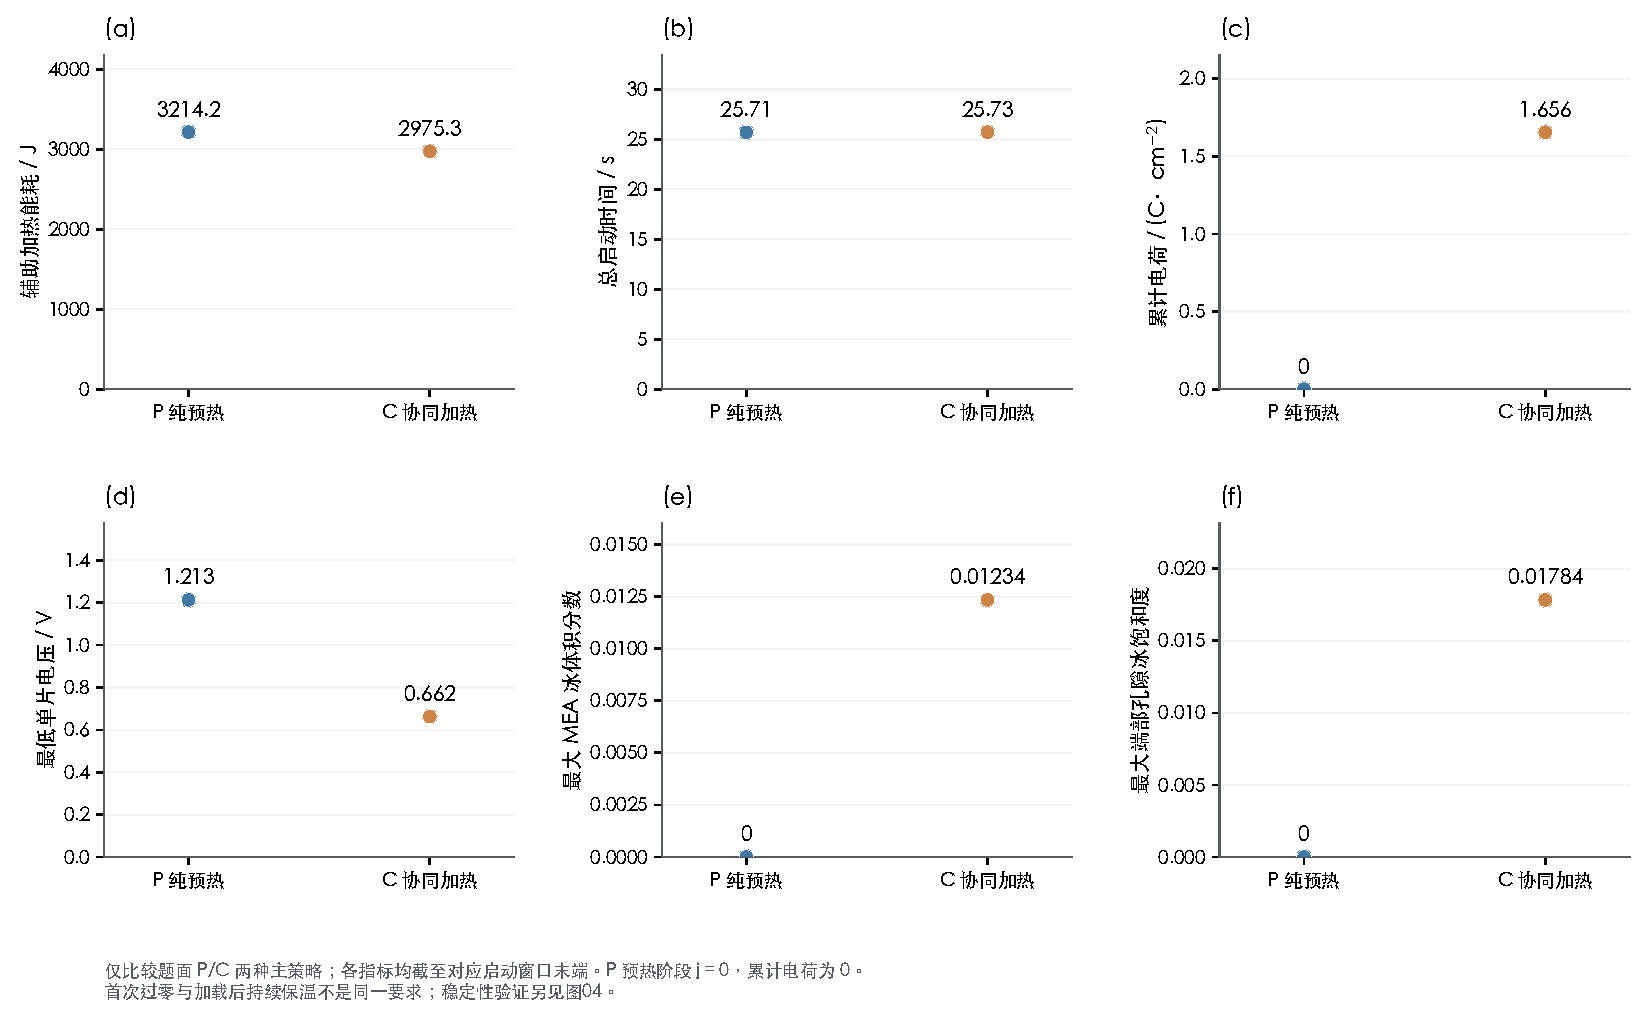
\includegraphics[width=.95\textwidth]{06_主策略关键指标对比.pdf}
\caption{两种主策略关键指标对比图}
\label{F6-1}
\end{figure}

图 \ref{F6-1}对两种主策略的能耗、启动时间、累计电荷、最低电压及冰量进行了汇总。可以看出，P 与 C 的首次启动时间分别为 25.71 s 和 25.73 s，差异不足 0.1 s，因此若仅按“五片单电池首次全部越过 \(0^\circ\mathrm C\)”的判据，两种策略的启动时间基本相当；但 C 策略从 \(t=0\) 即开始加载电流，在达到启动条件前已经累计输出 \(1.656\ \mathrm{C\,cm^{-2}}\) 的电荷，而 P 在整个预热阶段始终保持 \(j=0\)。因此，C 策略的优势并不主要体现为首次过零时间显著缩短，而是能够在升温的同时开始输出电能，实现“加热—发电”并行。

\subsubsection{温度演化与分片功率分配特征}
\begin{figure}[!h]
\centering
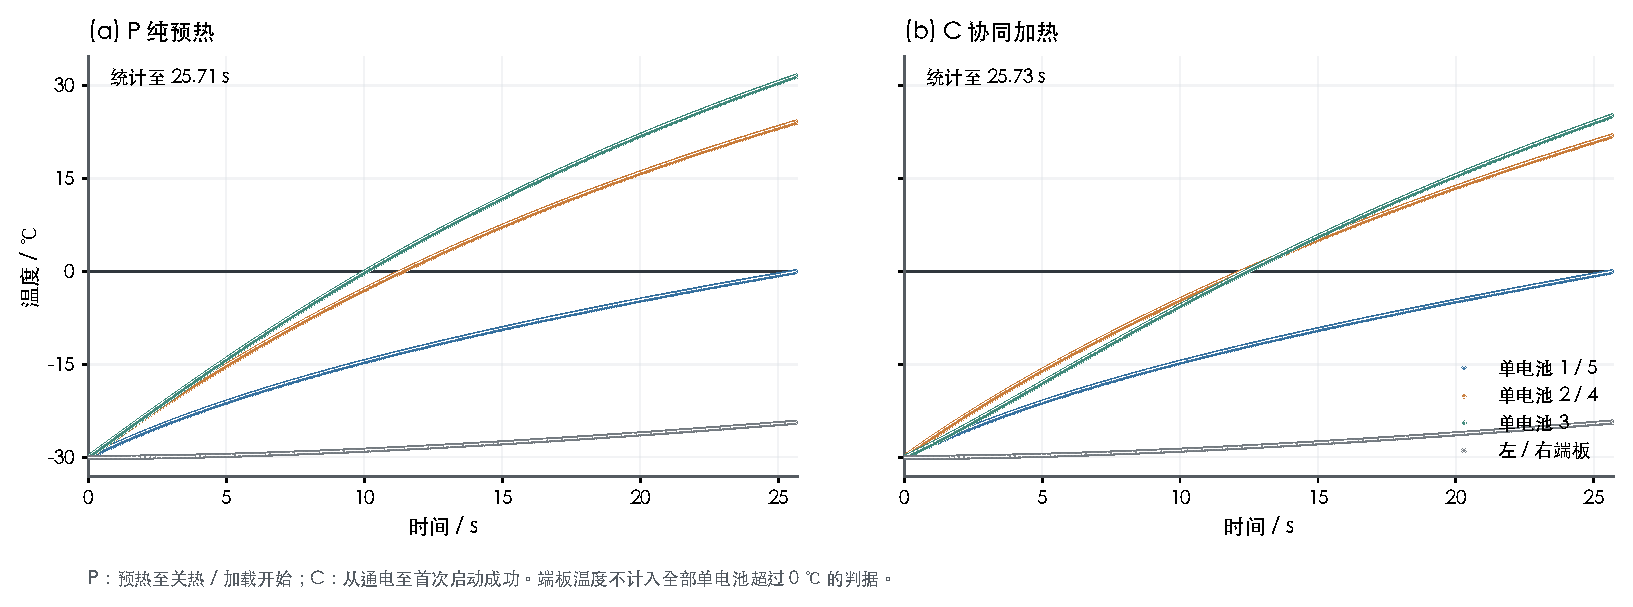
\includegraphics[width=.95\textwidth]{01_主策略温度历程.pdf}
\caption{两种主策略温度历程图}
\label{F6-2}
\end{figure}

由图 \ref{F6-2} 可见，两种策略下五片单电池均由 \(-30^\circ\mathrm C\) 持续升温，但由于端板热惯性和端部环境散热的存在，沿堆叠方向形成了明显的温度非均匀性。无论采用 P 还是 C，端部第 1、5 片始终为温升最慢的单电池，而中间区域温升更快，因此电堆是否达到启动条件最终由端部单电池决定。P 策略在约 25.71 s 时端部单电池刚越过冰点，此时第 2、4 片和中心第 3 片已经具有较高温度，而左右端板仍仅升至约 \(-24.3^\circ\mathrm C\)。这说明冷启动窗口内大量辅助热量首先用于提高单电池温度，而大热容端板的升温明显滞后，并持续作为端部单电池的低温热汇。 
C 策略的空间温度分布与 P 总体一致，但由于从 \(t=0\) 起已有电化学反应热参与升温，中心电池所需的外部辅助功率可以适当降低。由图 \ref{F6-1}(b) 可以看出，即使中心片加热功率降至约 \(0.6245\ \mathrm{W\,cm^{-2}}\)，其温度仍明显高于端部单电池，说明中心位置具有较好的热边界条件，不承担端板吸热和端部对流负荷，因此反应热与相邻单电池传热已能够补偿一部分辅助加热需求。

\begin{figure}[!h]
\centering
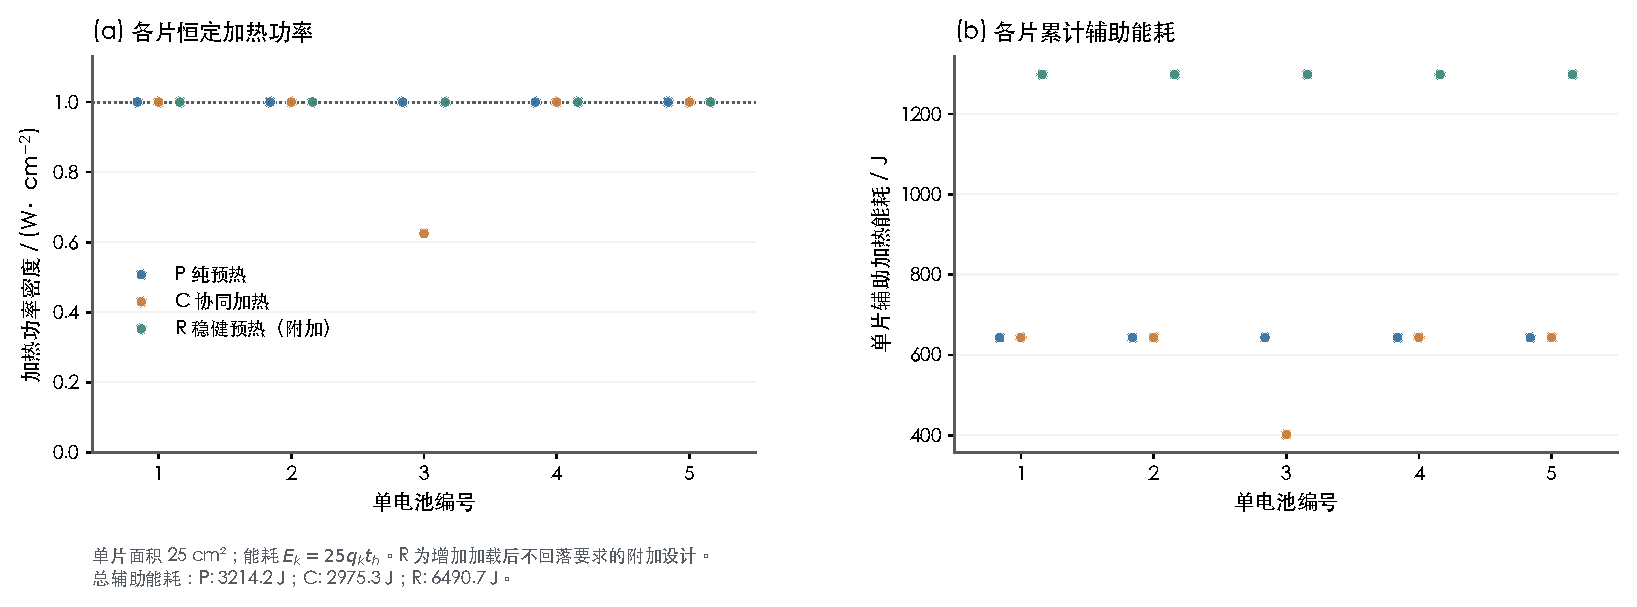
\includegraphics[width=.95\textwidth]{02_分片加热功率与能耗.pdf}
\caption{各片加热功率与辅助能耗分配图}
\label{F6-3}
\end{figure}

图 \ref{F6-3} 进一步说明了两种策略功率分配的差异。对于 P 策略，五片最优功率均达到上限 \(1\ \mathrm{W\,cm^{-2}}\)，对应各片能耗均为 \(642.8\,\mathrm J\)。这一结果与仅根据端板热汇所作的“端部功率应明显高于中心片”的简单判断并不一致。其原因在于完整电堆模型保留了片间导热，中间单电池获得的额外热量能够经相邻双极板向端部方向传递，因此提高中间片功率并非无效加热，而可以缩短限制全堆启动的端部过零时间。数值扫描进一步表明，当保持端部和次端功率为满功率、仅将中心片降至 \(0.5\ \mathrm{W\,cm^{-2}}\) 时，预热时间增加至 29.13 s，总能耗反而升至约 3277 J；若中心功率进一步降至 0.1，则启动时间增至 32.83 s、总能耗增至约 3365 J。由此表明，在纯预热条件下，“减少中心功率所节省的瞬时功率”不足以抵消“启动时间延长所增加的总能耗”，故最终最优解退化为五片全部满功率。  
与之不同，C 策略中各片从开始加载后均获得电化学反应热，中心片又不存在端部对流和端板吸热负担，因此其辅助功率可下降到 \(0.6245\ \mathrm{W\,cm^{-2}}\)，对应单片辅助能耗仅为 401.8 J；其余四片仍维持约 643.4 J。也就是说，C 策略的节能主要不是来自缩短总启动时间，而是来自反应热对升温负荷的分担以及对空间位置差异的功率重新分配。由图 \ref{F6-3} 可以直观看出，P 的能耗近似均匀分布，而 C 通过降低中心片功率，在保持端部快速升温的同时减少了不必要的中心加热。   

\subsubsection{电压变化、结冰过程及端部冰堵特性}

\begin{figure}[!h]
\centering
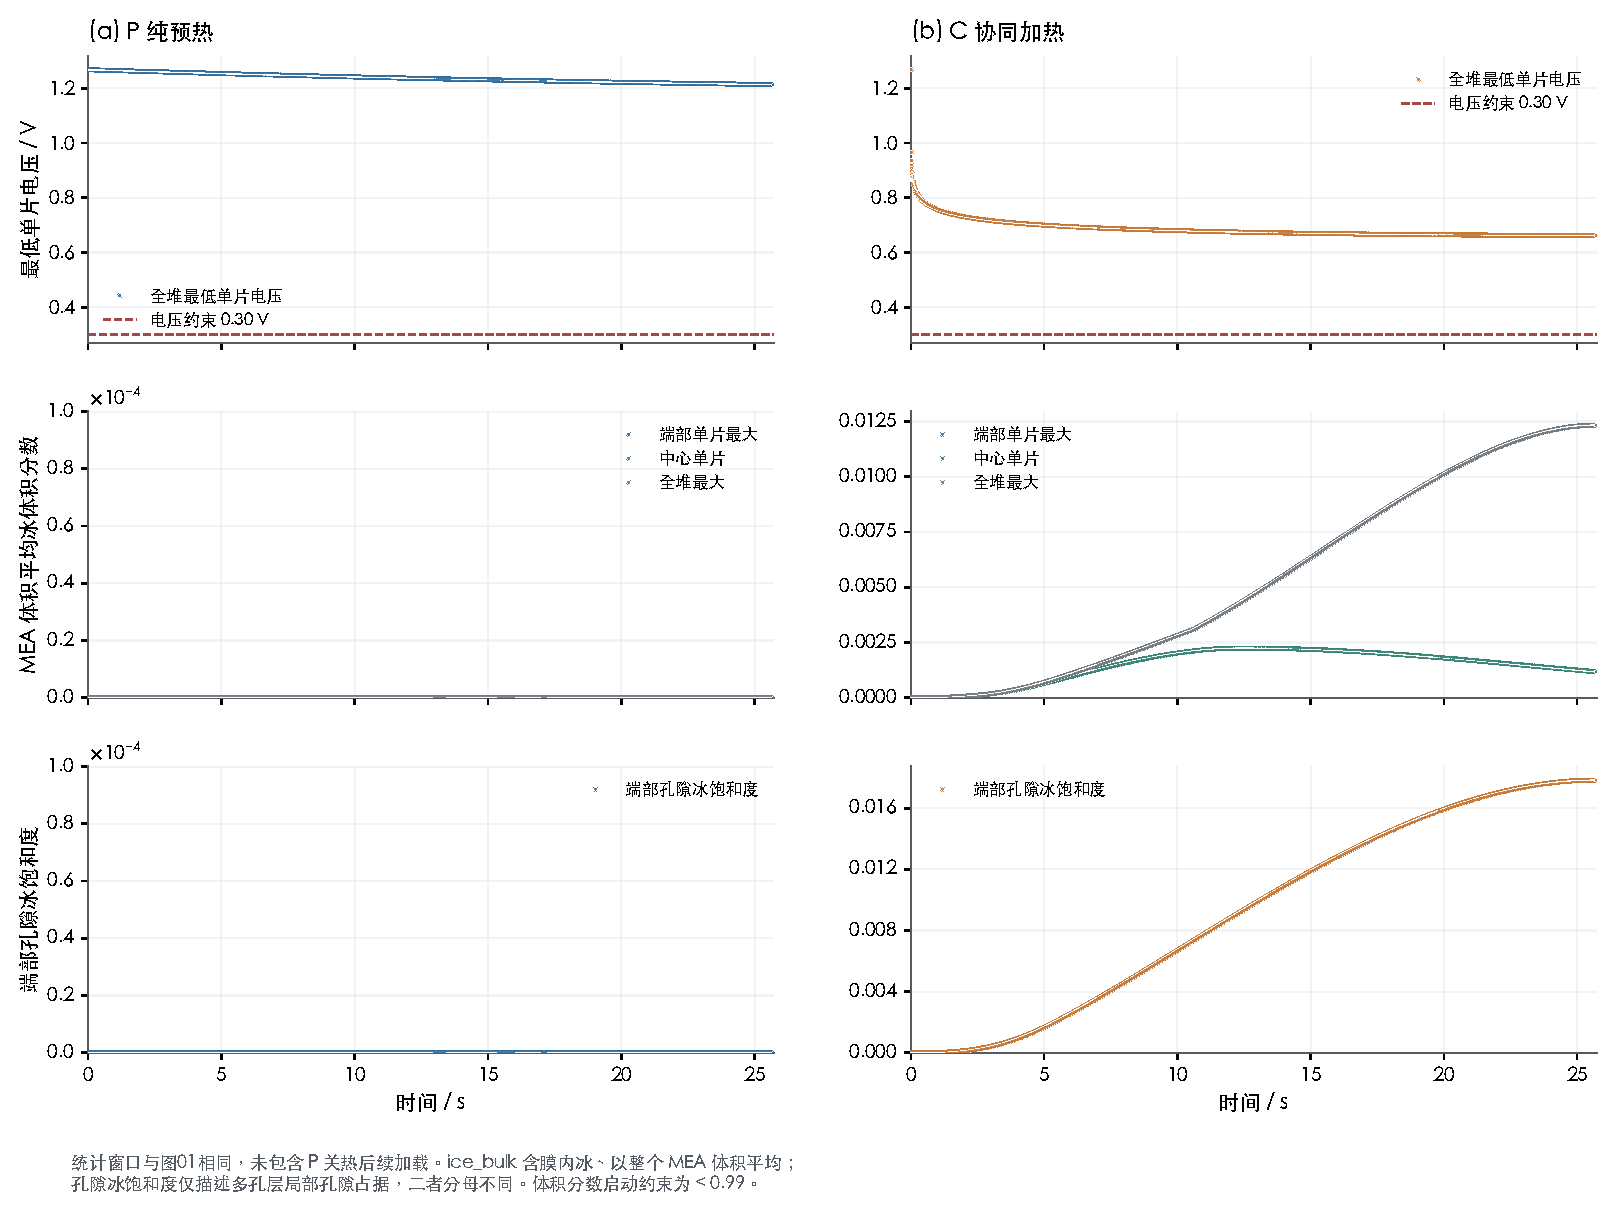
\includegraphics[width=.95\textwidth]{03_主策略电压与结冰.pdf}
\caption{各片加热功率与辅助能耗分配图}
\label{F6-4}
\end{figure}

除温升速度外，低温启动是否可行还取决于加载过程中单片电压及冰相积累是否越过安全边界。图 \ref{F6-4} 给出了两种策略启动窗口内的全堆最低单片电压、MEA 体积平均冰体积分数和端部孔隙冰饱和度。
对于 P 策略，由于整个预热阶段 \(j=0\)，各片处于近似开路状态，因此最低单片电压始终保持在较高水平，统计得到启动窗口内最低电压约为 1.213 V。与此同时，由于预热期间没有电化学反应产水，且启动前孔隙水已通过吹扫处理，MEA 平均冰体积分数仅为约 \(4.2\times10^{-20}\)，可视为零，端部孔隙冰饱和度同样近似为零。因此，纯预加热策略在首次启动窗口内几乎完全避免了低温产水—冻结过程，其突出优势是冰堵抑制能力最强。 
C 策略则表现出不同的水冰演化特征。由于电流从 \(t=0\) 开始加载，阴极随即生成反应水，而各片尚处于冰点以下，因此早期不可避免地出现“产水—冻结—升温”的竞争过程。由图 \ref{F6-4}(b) 可见，最低单片电压随电流增加逐步下降，启动时最低值约为 0.662 V，但全过程仍显著高于 0.30 V 的安全下限。与此同时，MEA 平均冰量在升温过程中逐步增加，其中全堆最大体积平均冰体积分数约为 0.01234，端部局部孔隙冰饱和度峰值约为 0.01784。两者均远低于严重冰堵阈值，说明虽然协同启动产生了可观测的早期结冰，但并未形成足以阻塞气体传输或触发电压失效的严重冰堵。   
还需注意，图 \ref{F6-4} 中“MEA 体积平均冰体积分数”与“端部孔隙冰饱和度”具有不同的物理含义。前者包含膜内冰，并以整个 MEA 体积为分母；后者只反映多孔层孔隙中冰所占比例。因此二者数值不能直接相互替代。当前结果中，C 策略的最大 MEA 冰体积分数为 0.0123、最大端部孔隙冰饱和度约 0.0178，均处于较低水平，说明其早期结冰属于可控范围，而非接近严重堵塞状态。   

综合表 \ref{tab:opt_results} 与图 \ref{F6-4}，可以得到两种策略最主要的权衡关系：P 通过“先升温、后产水”几乎完全避免冰生成，但全部升温负荷均由电热丝承担；C 通过“边发电、边加热”利用反应热降低外部能耗，但必须接受启动初期少量结冰。因此，就题目要求比较的端部冰堵抑制而言，P 明显优于 C；就辅助能耗而言，C 更具有优势。

\subsubsection{辅助能耗、启动速度及两种策略综合比较}
从总体性能来看，C 策略的辅助加热总能耗由 P 的 3214.2 J 降低到 2975.3 J，减少约 239 J。造成这一差异的主要原因不是两种策略的首次启动时间不同，而是 C 在 25.73 s 的启动窗口内额外获得了约 162.4 J 的反应产热，并通过降低中心片辅助功率进一步减少外部电能投入。相比之下，P 在 25.71 s 的预热窗口内反应产热为零，因此单电池温升、端板吸热和环境散热全部需要由辅助电热丝承担。  

在启动速度方面，两种策略的首次越冰时间分别为 25.71 s 和 25.73 s，几乎不存在差异，因此不能简单表述为“C 的首次启动时间显著短于 P”。但从实际输出过程看，P 在前 25.71 s 完全处于纯加热等待状态，而 C 从 \(t=0\) 起就按照规定电流曲线输出电流，到启动时已经累计通过约 \(1.66\ \mathrm{C\,cm^{-2}}\) 的电荷。因此，如果评价指标不仅考虑首次越冰，还考虑何时开始产生电能，则 C 具有更加明显的工程响应优势。该结果表明，对于本题给定的 \(-30^\circ\mathrm C\) 初始条件和 \(1\ \mathrm{W\,cm^{-2}}\) 功率上限，两类方案的温升极限主要由端部热负荷控制，而 C 的主要收益体现在降低辅助能耗和消除纯等待阶段。   

因此，若严格按照题面两种主策略进行比较，可以归纳为：在“首次五片单电池共同越过冰点”的启动口径下，两者启动时间基本相当；P 的结冰控制最好，但需消耗更多外部加热能量；C 则通过反应热参与和非均匀功率分配，将辅助能耗降低约 \(7.4\%\)，同时保持最低电压和最大冰量均处于安全范围。该结果直接回答了问题三第二小问中对能耗、启动速度和端部冰堵抑制效果的比较要求。

\subsubsection{关热后温度回落及稳健预热分析}
上述 P、C 主结果均按照题目中的“首次达到启动成功条件”进行统计。但从热动力学角度看，首次越过冰点并不意味着电热丝关闭后电堆能够立即稳定维持在冰点以上。由于启动时端板仍明显低于 \(0^\circ\mathrm C\)，关热后端板继续从端部单电池吸收热量，而规定电流曲线初期的反应产热较小，因此可能出现明显的“加载即回落”现象。为检验这一问题，在主结果之外进一步采用相同的电流爬升曲线，对关热后的状态持续计算至累计电荷达到 \(20\ \mathrm{C\,cm^{-2}}\)。

\begin{figure}[!h]
\centering
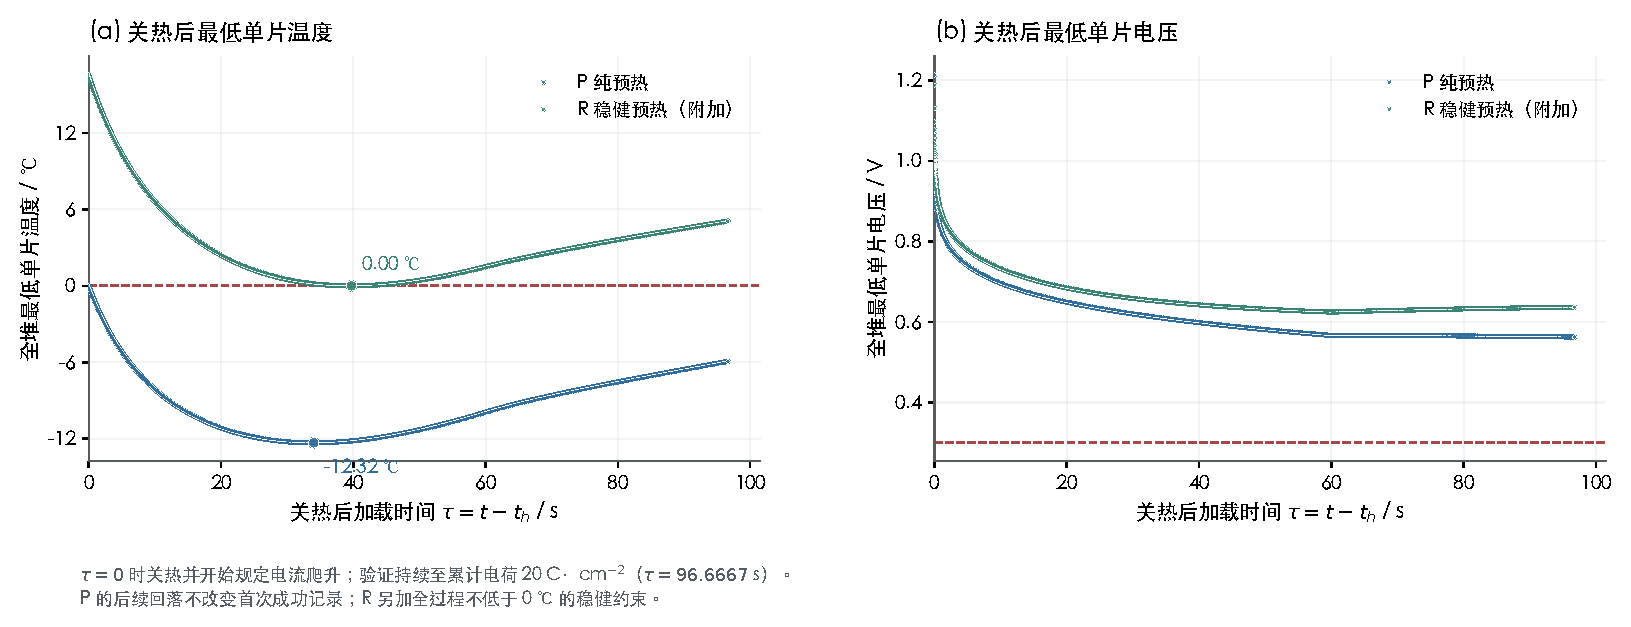
\includegraphics[width=.95\textwidth]{04_关热后回落与稳健验证.pdf}
\caption{关热后温度回落与稳健预热验证图}
\label{F6-5}
\end{figure}

由图 \ref{F6-5} 可见，P 策略在 25.71 s 首次过零后立即关热并开始加载时，全堆最低单片温度迅速再次降至冰点以下，最低约为 \(-12.32^\circ\mathrm C\)；C 策略关热后同样发生回落，后验计算最低温度约为 \(-9.57^\circ\mathrm C\)。虽然两种方案后续最低单片电压仍分别保持在约 0.563 V 和 0.565 V，未触发 0.30 V 的电压失效，但重新进入低温区域后冰量明显增加，说明“首次过零”和“关热后持续处于冰点以上”是两个不同层次的要求。   

为进一步考察对持续运行更严格的要求，设置附加稳健预热方案 R。该方案仍采用纯预热形式，但要求电热丝关闭后按照同一电流曲线运行完整 \(96.67\,\mathrm s\) 的过程中，全堆最低单片温度始终不低于 \(0^\circ\mathrm C\)。优化结果表明，需要将预热时间由 25.71 s 延长至 51.93 s，五片电热丝保持满功率，此时辅助加热总能耗增加至 6490.7 J。关热时端板已被加热至约 \(-0.58^\circ\mathrm C\)，后续加载过程中最低单片温度仅下降到约 \(0.001^\circ\mathrm C\)，没有再次跌破冰点，冰量也保持近似为零。  

需要强调的是，R 并不是题面规定的第三种辅助启动策略，而是针对主策略 P 的附加稳健性验证，因此不应与表 \ref{tab:opt_results}中 P、C 两种主策略并列作为问题三正式比较对象。其意义在于揭示端板热惯性对实际持续启动能力的影响：若仅要求“首次越冰”，约 3 kJ 的辅助能量即可完成启动；若进一步要求关热后在完整加载过程中不再跌回冰点以下，则必须显著提高端板温度，辅助能耗接近翻倍。这一结果也说明了问题四引入动态加热控制的必要性，即在达到首次启动条件后，不宜简单将辅助热源完全关闭，而应依据单片温度和电压状态进行逐步退热。

\subsubsection{能量收支与结果可靠性分析}
\begin{figure}[!h]
\centering
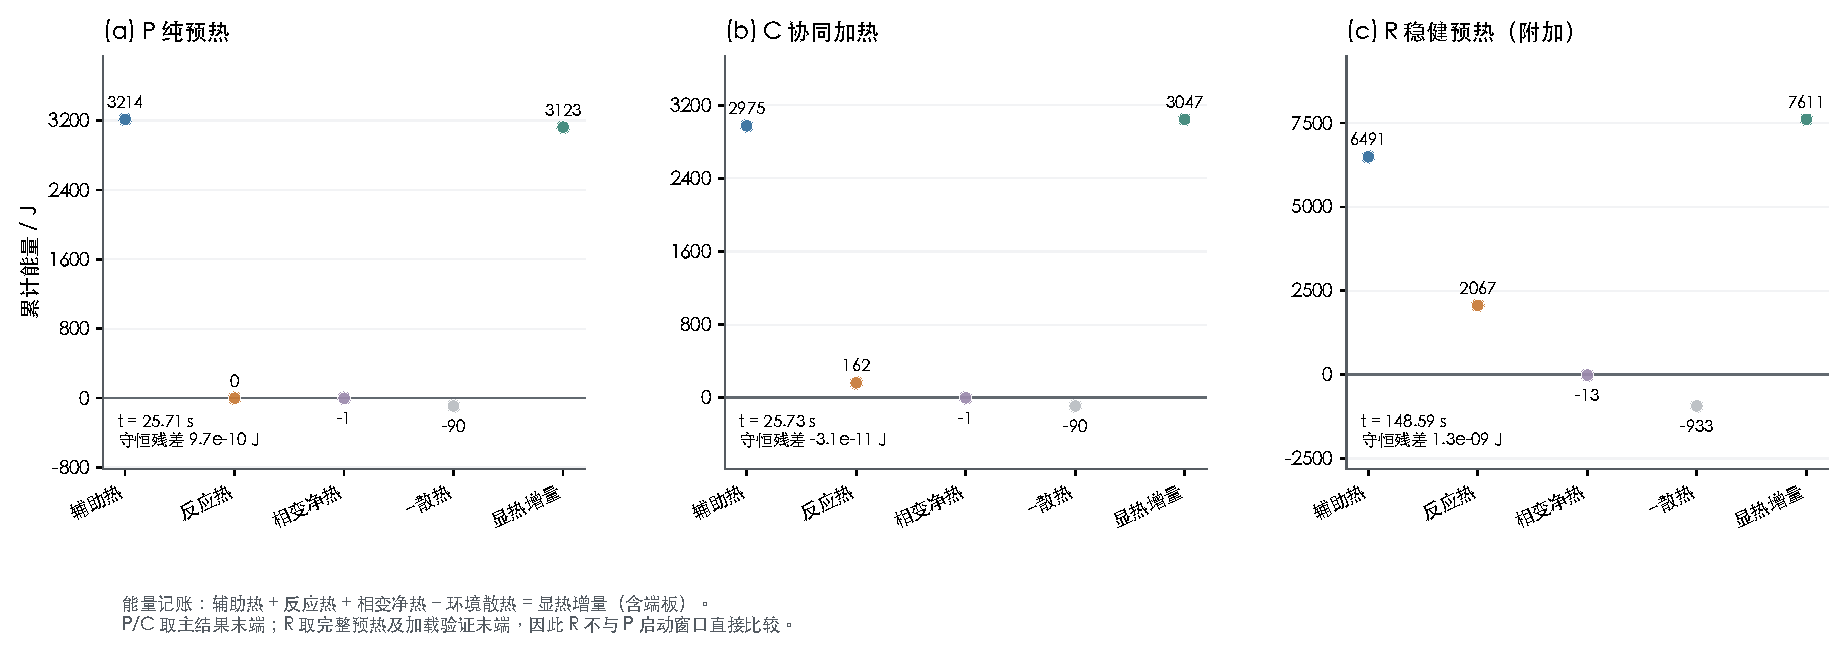
\includegraphics[width=.95\textwidth]{05_能量预算与守恒.pdf}
\caption{辅助冷启动能量预算与守恒检验图}
\label{F6-6}
\end{figure}
图 \ref{F6-6} 给出了两种主策略及附加稳健方案的全堆累计能量收支。按照 6.2 建立的整体能量守恒关系，辅助热、电化学反应热和相变净热扣除环境散热后，应等于包括端板在内的电堆显热增量。
对于 P 策略，在 25.71 s 的预热窗口内，辅助热输入为 3214.2 J，由于 \(j=0\)，反应热为零；相变净热约为 \(-1.07\) J，环境累计散热约为 90.06 J，因此最终显热增量约为 3123.1 J。对应能量平衡残差仅为 \(9.7\times10^{-10}\) J。对于 C 策略，辅助热为 2975.3 J，同时获得约 162.4 J 的电化学反应热，相变净热约为 \(-0.92\) J、环境散热约为 89.73 J，最终显热增量约为 3047.0 J，能量残差仅为 \(-3.1\times10^{-11}\) J。由此可见，C 策略所减少的辅助能耗与其反应热贡献及中心片功率降低相互对应，具有清晰的能量来源。

附加稳健方案 R 的完整预热及后续加载验证持续至 148.59 s。在该完整窗口内，累计辅助热约为 6491 J、反应热约为 2067 J、相变净热约为 \(-13\) J、环境散热约为 933 J，最终显热增量约为 7611 J，能量残差约为 \(1.3\times10^{-9}\) J。由于这一统计窗口包括 51.93 s 预热及之后的完整加载过程，因此不能直接与 P、C 的首次启动窗口能耗进行横向比较，其主要作用是验证较长时间尺度下模型的能量闭合。   

除热量守恒外，数值结果中的水量收支残差约为 \(10^{-15}\sim10^{-18}\) kg，左右对称位置的温度差保持在 \(10^{-12}\sim10^{-13}\) K 量级，说明水冰状态更新、片间热传递以及镜面对称结构均得到了良好保持。与此同时，时间步和空间网格加密结果显示，P、C、R 三种计算的辅助能耗分别稳定在 3214.1977 J、2975.2579 J 和 6490.6741 J；随着时间步减小和空间网格加密，首次启动时刻分别收敛到约 25.71 s、25.73 s 和 51.93 s，最低电压、最大冰量和端板终温也均单调趋于稳定，无明显数值振荡。  

为进一步判断主要结论对模型参数的依赖程度，对端板耦合导度 \(g_E\)、端板热容、环境对流系数 \(h\) 及冻结速率 \(k_f\) 进行扰动。结果表明，端板耦合导度是影响辅助能耗最显著的参数：当 \(g_E\) 降低 20\% 时，P 的辅助能耗由约 3215 J 降至 2776 J，而提高 20\% 后增至 3670 J；C 的辅助能耗也相应由约 2976 J 变化至 2583 J 和 3375 J。这再次说明端板吸热是限制极低温冷启动的主要热力学因素。相比之下，冻结速率主要影响 C 策略的早期冰峰，而对能耗几乎没有影响；即使将 \(k_f\) 放大 100 倍，C 的最大冰体积分数也仅增加到约 0.0525，仍远低于严重冰堵阈值。因此，两种主策略在能耗和冰堵方面的相对结论对主要参数扰动具有较好的稳定性。  

综上，问题三的优化结果表明：在 \(-30^\circ\mathrm C\) 条件下，两种辅助加热方式均可以使五片电堆完成首次冷启动。纯预加热策略通过在产水前完成升温，能够将启动窗口内的冰量控制在近似为零的水平，但需要五片电热丝同时满功率工作，总辅助能耗较高；恒定功率协同策略利用反应热参与升温，并根据不同位置的热负荷对功率进行非均匀分配，使辅助能耗降低至 2975.3 J，同时保持最低电压和最大冰量均满足安全约束。两者在首次越冰时间上基本相当，但 C 从启动初期即可输出电流，因此在实际快速供能方面更具优势。与此同时，关热后的后验验证说明，首次越冰并不代表电堆已经获得足够热裕度，端板热惯性仍可能使端部单电池重新跌回冰点以下，这为下一问进一步采用基于温度、电压反馈的动态辅助加热策略提供了直接依据。


\subsection{问题三小结}
针对 \(-30^\circ\mathrm C\) 极低温条件下电堆仅依靠电化学反应产热难以实现冷启动的问题，本文在问题二五片电堆瞬态水—冰—热—电耦合模型基础上，在各片双极板内引入独立可调的电热丝，将辅助热源并入七节点热网络，并建立了对应的辅助加热能耗模型。在此基础上，分别构建纯预加热和恒定功率协同两类辅助冷启动策略，以各片加热功率密度及加热持续时间为决策变量，在温度、电压、冰体积分数和累计电荷量等约束下，以辅助加热总能耗最小为目标完成优化求解。

结果表明，纯预加热策略采用五片满功率加热，在约 \(25.71\,\mathrm s\) 时完成首次启动，总辅助能耗为 \(3214.2\,\mathrm J\)，启动窗口内冰量近似为零；恒定功率协同策略的最优功率分配为 \((1,1,0.6245,1,1)\ \mathrm{W\,cm^{-2}}\)，约 \(25.73\,\mathrm s\) 完成启动，总辅助能耗降至 \(2975.3\,\mathrm J\)，且最低单片电压和最大冰体积分数均满足安全约束。由此可见，协同启动能够利用反应热分担升温负荷，降低辅助能耗并从启动初期输出电流，而纯预加热在抑制低温结冰方面更具优势。此外，关热后的后验分析表明，端板热惯性可能导致单电池再次跌回冰点以下，因此后续仍需根据单片实时状态动态调节辅助加热功率，为问题四的反馈控制策略建立基础。

\section{问题四的分析与求解}

\subsection{问题描述和分析}

问题四要求在问题三恒定功率协同启动模型的基础上，进一步允许各片电热丝功率随时间独立调节，利用单片温度、电压及其变化信息设计动态辅助加热策略，并在满足冷启动成功与安全约束的条件下，以辅助加热总能耗最小为主要目标，比较不同预冷工况下动态控制与恒功率控制的启动性能。同时，还需建立电堆由常温向低温环境冷却的传热模型，研究预冷时间对初始温度场及后续恒功率冷启动结果的影响。

与前一问相比，本问的关键变化在于初始状态由均匀低温扩展为预冷形成的非均匀温度场，辅助加热则由固定功率输入转变为根据运行状态实时调整的反馈控制。预冷程度决定电堆的初始储热量及端部与中部的温度差异；启动过程中，各片温升、反应产水与结冰状态又随电流加载和辅助功率不断变化。因此，固定功率难以同时适应不同初温及各片的瞬时热量需求，而动态控制需要在增强低温单片加热、抑制冰堵风险与接近目标时及时降功率之间进行协调。

基于上述特点，本文首先建立复合层状电堆的预冷传热模型，将其终态温度场映射为五片单电池及两块端板的初始温度；随后在已有水—冰—热—电耦合模型基础上，引入温度、电压滤波与独立状态观测，构建前馈与PI反馈相结合的分片功率控制律，并通过离线参数搜索确定节能且具有一定安全裕度的控制方案。最后，在统一电流加载、成功判据和评价窗口下比较三种预冷工况的启动结果，并通过预冷时间扫描分析初始储热、片间温差与冷启动性能之间的关系。

\subsection{电堆预冷与动态辅助冷启动模型的建立}

问题四继续采用第五章的七节点电堆热网络和第六章的辅助热源模型，各片内部水冰相变、气体输运、极化损失及电压计算关系保持一致。本问新增的模型包括预冷初始温度场、仅依赖可测信号的状态识别，以及随时间更新的分片辅助功率。为区分两个先后发生的过程，以 $\tau$ 表示预冷时间，以 $t$ 表示电流加载后的启动时间；预冷结束时重新令 $t=0$，并将预冷终态作为冷启动初态。以下物理方程中的温度统一采用开尔文，表格和图中的温度则用摄氏度表示；控制器中的温度差和温升速率不受温标平移影响，使用摄氏度实现时只需将冰点设为零。

\subsubsection{预冷传热模型及初边界条件}

电堆在预冷阶段不加载电流，各片电热丝均关闭，内部不存在电化学反应产热。沿用吹扫后的初始状态，忽略该阶段的水相变及辐射换热，仅考虑沿堆叠方向的导热和端板外表面与环境之间的对流。五片电堆由两块端板、六块双极板及五片MEA组成，其中每片MEA仍分为阳极气体扩散层、阳极催化层、质子交换膜、阴极催化层和阴极气体扩散层，共形成33个实际材料区。内部双极板由相邻单电池共享，不重复计算其厚度和热质量。因此，整堆厚度为
\begin{equation}
L_s=2L_{\mathrm{EP}}+6L_{\mathrm{BP}}+5L_{\mathrm{MEA}}
=2\times10+6\times2+5\times0.3267=33.6335\ \mathrm{mm}.
\tag{7-1}\label{eq:q4:stack_length}
\end{equation}

在第 $j$ 个材料区 $\Omega_j$ 内，采用附件给定的密度、比热容与导热系数，温度场满足
\begin{equation}
(\rho c_p)_j\frac{\partial T}{\partial\tau}
=\frac{\partial}{\partial x}\left(k_j\frac{\partial T}{\partial x}\right),
\qquad x\in\Omega_j,\quad 0<x<L_s.
\tag{7-2}\label{eq:q4:precool_pde}
\end{equation}

相邻材料间取理想热接触，界面处温度和导热通量连续，即
\begin{equation}
T(x_j^-,\tau)=T(x_j^+,\tau),\qquad
k_j\left.\frac{\partial T}{\partial x}\right|_{x_j^-}
=k_{j+1}\left.\frac{\partial T}{\partial x}\right|_{x_j^+}.
\tag{7-3}\label{eq:q4:precool_interface}
\end{equation}

两端对流边界按照向外散热为正确定符号。由于左端外法向与 $x$ 轴正方向相反，左右边界分别为
\begin{equation}
\left\{\begin{aligned}
k_{\mathrm{EP}}\left.\frac{\partial T}{\partial x}\right|_{x=0}
&=h\big[T(0,\tau)-T_{\mathrm{amb}}\big],\\
-k_{\mathrm{EP}}\left.\frac{\partial T}{\partial x}\right|_{x=L_s}
&=h\big[T(L_s,\tau)-T_{\mathrm{amb}}\big],
\end{aligned}\right.
\qquad h=40\ \mathrm{W\,m^{-2}K^{-1}}.
\tag{7-4}\label{eq:q4:precool_robin}
\end{equation}

预冷开始时全堆为均匀常温，环境温度恒为 $-30^\circ\mathrm C$，故初始条件为
\begin{equation}
T(x,0)=T_{\mathrm{init}}=298.15\ \mathrm K,\qquad
T_{\mathrm{amb}}=243.15\ \mathrm K.
\tag{7-5}\label{eq:q4:precool_initial}
\end{equation}

数值计算保留MEA的五层材料结构。为分析电堆热惯性，仍可将其单位面积热容与串联热阻分别合并为
\begin{equation}
\begin{aligned}
C_{A,\mathrm{MEA}}&=\sum_{\ell\in\mathrm{MEA}}(\rho c_p)_\ell L_\ell
=60.75966\ \mathrm{J\,m^{-2}K^{-1}},\\
k_{\mathrm{MEA}}^{\mathrm{eq}}&=\frac{L_{\mathrm{MEA}}}{\displaystyle\sum_{\ell\in\mathrm{MEA}}L_\ell/k_\ell}
\approx0.296\ \mathrm{W\,m^{-1}K^{-1}},\\
C_{A,\mathrm{tot}}&=2C_{A,\mathrm{EP}}+6C_{A,\mathrm{BP}}+5C_{A,\mathrm{MEA}}
=97503.96\ \mathrm{J\,m^{-2}K^{-1}}.
\end{aligned}
\tag{7-6}\label{eq:q4:precool_capacity}
\end{equation}

其中，单块端板与双极板的面热容分别为 $39500$ 和 $3033.36\ \mathrm{J\,m^{-2}K^{-1}}$，两块端板合计约占全堆热容的 $81\%$。因此，预冷温度不仅取决于MEA本身，还受到板体储热及端部散热过程的显著影响，不能仅以单片初始温度的统一平移代替完整预冷计算。

\subsubsection{非均匀初始温度场与电堆热网络的衔接}

预冷模型得到的是沿堆叠方向连续分布的温度场，而启动模型采用五个单电池温度和两个独立端板温度。为保持两种空间描述之间的热量对应关系，将每块内部共享双极板沿几何中面等分，并分别归入左右相邻单电池；两块终端双极板全部归入相应端部单电池，端板则保留独立节点。记第 $a$ 个热节点所属空间范围为 $\Omega_a$，预冷持续时间为 $\tau_c$，则节点初始温度取热容加权平均：
\begin{equation}
\begin{aligned}
T_a^0&=\frac{\displaystyle\int_{\Omega_a}\rho(x)c_p(x)T(x,\tau_c)\,\mathrm dx}
{\displaystyle\int_{\Omega_a}\rho(x)c_p(x)\,\mathrm dx}
=\frac{\displaystyle\sum_{i\in\Omega_a}C_iT_i(\tau_c)}
{\displaystyle\sum_{i\in\Omega_a}C_i},\\
C_i&=(\rho c_p)_i\Delta x_i.
\end{aligned}
\tag{7-7}\label{eq:q4:temperature_map}
\end{equation}

由于各控制体只归属于一个节点，式\eqref{eq:q4:temperature_map}满足预冷物性下的显热恒等关系
\begin{equation}
\sum_{a=1}^{7}C_{A,a}^{\mathrm{pre}}(T_a^0-T_{\mathrm{amb}})
=\sum_iC_i\big[T_i(\tau_c)-T_{\mathrm{amb}}\big],\qquad
C_{A,a}^{\mathrm{pre}}=\sum_{i\in\Omega_a}C_i.
\tag{7-8}\label{eq:q4:map_energy}
\end{equation}

由此构造完全冷却、预冷20 min和预冷40 min三种初态。为便于数值组装，将七节点状态排列为 $\boldsymbol T=[T_1,T_2,T_3,T_4,T_5,T_{\mathrm{EL}},T_{\mathrm{ER}}]^{\mathrm T}$，记上述映射为 $\mathcal M$，则
\begin{equation}
\boldsymbol T^0=\begin{cases}
T_{\mathrm{amb}}\boldsymbol 1, & \text{完全冷却工况},\\
\mathcal M[T(x,1200\ \mathrm s)], & \text{预冷20 min工况},\\
\mathcal M[T(x,2400\ \mathrm s)], & \text{预冷40 min工况}.
\end{cases}
\tag{7-9}\label{eq:q4:three_initial_states}
\end{equation}

启动时各片孔隙液水和冰初值仍取零，膜初始含水量取 $\lambda_0=3$。各片气体、水冰及膜水状态组成内部状态向量 $\boldsymbol X$，随后按第四至第六章的方程演化。辅助功率改为随时间变化后，七节点能量方程可统一写为
\begin{equation}
\begin{aligned}
\boldsymbol C(\boldsymbol X)\frac{\mathrm d\boldsymbol T}{\mathrm dt}
&=-\boldsymbol G(\boldsymbol X)\boldsymbol T
+\boldsymbol hT_{\mathrm{amb}}+\boldsymbol b_{\mathrm{gen}}
+\boldsymbol b_{\mathrm{pc}}+10^4\boldsymbol B\boldsymbol q(t),\\
b_{\mathrm{gen},k}&=10^4j(t)\big(E_{\mathrm{th}}-V_k\big),\qquad
E_{\mathrm{th}}=1.48\ \mathrm V,\qquad k=1,\ldots,5.
\end{aligned}
\tag{7-10}\label{eq:q4:plant_heat}
\end{equation}

其中，$\boldsymbol B$ 将五片电热丝功率输入对应单电池节点，其端板行均为零；$\boldsymbol G$ 包含片间、片板导热及环境散热，$\boldsymbol b_{\mathrm{pc}}$ 表示水相变化的热效应。$j$ 与 $q_k$ 分别以 $\mathrm{A\,cm^{-2}}$ 和 $\mathrm{W\,cm^{-2}}$ 计，因而进入单位面积热网络时均须乘以 $10^4$。

这里保留了前章启动模型的两项继承设置：启动阶段采用含水气有效物性的节点热容，对流散热作用于首尾单电池节点；预冷阶段则采用附件材料热容，对流作用于实际端板外表面。因此，式\eqref{eq:q4:map_energy}保证预冷温度场在其自身物性下的热量加权一致性，但不意味着两阶段具有完全相同的热容或严格相同的初始焓。这一处理使不同辅助控制策略能够在同一启动模型上比较，其近似影响通过后续传热参数扰动与数值检验加以考察。

\subsubsection{温度、电压反馈与单电池运行状态识别}

控制器可直接获取的反馈量为各片温度和电压，冰含量及端板温度则需通过模型估计。为避免将仿真中的真实内部状态作为控制输入，另设具有独立水、气和热状态的名义模型观测器。观测器由已知电流与上一时段实际施加的加热功率推进，每个采样时刻仅用测得的五片温度校正对应温度节点；其端板温度及内部水气状态保留模型预测值。记控制时刻 $t_n=n\Delta t_c$，可写为
\begin{equation}
\begin{aligned}
\widehat{\boldsymbol x}^{\,n,-}
&=\mathcal P_{\widehat{\boldsymbol p}}\!\left(
\widehat{\boldsymbol x}^{\,n-1,+},j|_{[t_{n-1},t_n]},\boldsymbol q^{n-1},\Delta t_c\right),
\\
\widehat T_k^{n,+}&=T_{k,\mathrm m}^n,\qquad k=1,\ldots,5.
\end{aligned}
\tag{7-11}\label{eq:q4:independent_observer}
\end{equation}

式中，$\widehat{\boldsymbol p}$ 为名义物性参数，$\mathcal P$ 表示水—热—电耦合模型的预测算子；实际电堆中的冰、水、气库存和扰动物性均不传入观测器。其预测电压 $\widehat V_k^n$ 由独立内部状态、采样温度与已知电流共同计算，作为后续冰风险修正的依据。

为减弱采样噪声对控制动作的影响，首先对测温和测压信号进行一阶低通滤波：
\begin{equation}
\begin{aligned}
\widetilde T_k^n&=\beta\widetilde T_k^{n-1}+(1-\beta)T_{k,\mathrm m}^n,\\
\widetilde V_k^n&=\beta\widetilde V_k^{n-1}+(1-\beta)V_{k,\mathrm m}^n,
\qquad \beta=\exp\!\left(-\frac{\Delta t_c}{0.15\ \mathrm s}\right).
\end{aligned}
\tag{7-12}\label{eq:q4:signal_filter}
\end{equation}

再由滤波信号的后向差分估计温升速率与电压变化率，并对差分结果继续滤波：
\begin{equation}
\begin{aligned}
r_{T,k}^n&=\beta_r r_{T,k}^{n-1}+(1-\beta_r)
\frac{\widetilde T_k^n-\widetilde T_k^{n-1}}{\Delta t_c},\\
r_{V,k}^n&=\beta_r r_{V,k}^{n-1}+(1-\beta_r)
\frac{\widetilde V_k^n-\widetilde V_k^{n-1}}{\Delta t_c},\qquad
\beta_r=\exp\!\left(-\frac{\Delta t_c}{0.20\ \mathrm s}\right).
\end{aligned}
\tag{7-13}\label{eq:q4:rate_filter}
\end{equation}

设 $\widehat\varepsilon_{k,\mathrm{mod}}^n$ 为独立模型给出的片内最大冰体积分数，采用预测电压与测量电压的有符号残差修正冰风险标量：
\begin{equation}
\begin{aligned}
\widehat\varepsilon_k^n
&=\operatorname{sat}_{[0,1]}\!\left[
\widehat\varepsilon_{k,\mathrm{mod}}^n
+L_\varepsilon\frac{\widehat V_k^n-V_{k,\mathrm m}^n}{\delta V_{\mathrm{obs}}}\right],
\\
&\qquad L_\varepsilon=0.02,\quad\delta V_{\mathrm{obs}}=0.10\ \mathrm V.
\end{aligned}
\tag{7-14}\label{eq:q4:ice_estimator}
\end{equation}

其中，$\operatorname{sat}_{[a,b]}(z)=\min\{b,\max(a,z)\}$。当实测电压低于模型预测时，修正项提高冰风险估计；反向残差则降低估计值。该修正只作用于控制器使用的风险标量，不直接改写观测器的水冰库存，也不等价于从电压唯一重建真实冰场。

以 $T_f=273.15\ \mathrm K$ 表示冰点，$T_{\mathrm{targ}}$ 和 $t_{\mathrm{plan}}$ 分别表示参考目标温度和规划升温时间。温度偏低程度、当前所需温升速率及温升不足程度定义为
\begin{equation}
\begin{aligned}
D_{T,k}^n&=\max\!\left(0,\frac{T_f-\widetilde T_k^n}{30\ \mathrm K}\right),\\
r_{\mathrm{req},k}^n&=\max\!\left(0,\frac{T_{\mathrm{targ}}-\widetilde T_k^n}
{\max(t_{\mathrm{plan}}-t_n,1\ \mathrm s)}\right),\\
D_{r,k}^n&=\max\!\left(0,\frac{r_{\mathrm{req},k}^n-r_{T,k}^n}
{r_{\mathrm{req},k}^n+0.01\ \mathrm{K\,s^{-1}}}\right).
\end{aligned}
\tag{7-15}\label{eq:q4:temperature_deficit}
\end{equation}

进一步将冰量估计、电压裕度和电压下降速率组合为风险指标
\begin{equation}
\begin{aligned}
R_k^n={}&0.4\frac{\widehat\varepsilon_k^n}{\varepsilon_{\mathrm{crit}}}
+0.4\max\!\left(0,\frac{V_{\mathrm{safe}}+\delta_V-\widetilde V_k^n}{\delta_V}\right)
\\
&{}+0.2\min\!\left(1,\frac{\max(0,-r_{V,k}^n)}{0.10\ \mathrm{V\,s^{-1}}}\right).
\end{aligned}
\tag{7-16}\label{eq:q4:ice_risk}
\end{equation}

其中，$V_{\mathrm{safe}}=0.30\ \mathrm V$、$\varepsilon_{\mathrm{crit}}=0.99$ 为安全阈值，$\delta_V=0.10\ \mathrm V$ 为电压预警带宽。当冰量、电压、下降速率或综合风险任一项触发预警时，判为需要优先增强加热：
\begin{equation}
\begin{aligned}
\mathcal D_k^n={}&
\big\{\widehat\varepsilon_k^n>0.8\big\}
\ \cup\ \big\{\widetilde V_k^n<0.40\ \mathrm V\big\}
\ \cup\ \big\{R_k^n>0.7\big\}\\
&{}\cup\ \big\{r_{V,k}^n<-0.10\ \mathrm{V\,s^{-1}},\
\widetilde V_k^n<0.60\ \mathrm V\big\}.
\end{aligned}
\tag{7-17}\label{eq:q4:danger_condition}
\end{equation}

上述判据将低温但温升正常、温升不足、冰堵或低压风险以及接近目标等情形区分开来，使控制器能够依据当前状态分配辅助功率。其作用是提前响应风险，是否真正满足题设安全约束仍须由被控对象的真实状态独立检验。

\subsubsection{前馈与PI结合的动态功率控制律}

动态控制以参考温升轨迹为基本目标，在初期弥补升温所需热量，在临近目标时降低输入，并在低压或冰堵预警时保留安全增强通道。各片采用自身初温建立分段线性参考轨迹：
\begin{equation}
\begin{aligned}
T_{\mathrm{ref},k}(t)&=T_k^0+
(T_{\mathrm{targ}}-T_k^0)\min\!\left(\frac{t}{t_{\mathrm{plan}}},1\right),
\\
\dot T_{\mathrm{ref},k}(t)&=\begin{cases}
(T_{\mathrm{targ}}-T_k^0)/t_{\mathrm{plan}}, & t<t_{\mathrm{plan}},\\
0, & t\geq t_{\mathrm{plan}}.
\end{cases}
\end{aligned}
\tag{7-18}\label{eq:q4:temperature_reference}
\end{equation}

目标温度和规划时间作为离线搜索参数，不预先假定某一轨迹具有全局最优性。以滤波温度构造跟踪误差，并根据低温程度调整比例增益：
\begin{equation}
e_k^n=T_{\mathrm{ref},k}(t_n)-\widetilde T_k^n,
\qquad
K_{P,k}^n=K_P\big[0.6+0.4\min(1,D_{T,k}^n)\big].
\tag{7-19}\label{eq:q4:tracking_error_gain}
\end{equation}

前馈项利用独立模型的节点热容、导热损失、估计端板温度及反应产热，补偿沿参考轨迹升温时的净热量缺口：
\begin{equation}
\begin{aligned}
q_{\mathrm{ff},k}^n
&=\frac{\alpha_{\mathrm{ff}}}{10^4}
\left[\widehat C_{A,k}^n\dot T_{\mathrm{ref},k}(t_n)
+\widehat\ell_k^n-10^4j(t_n)\big(E_{\mathrm{th}}-V_{k,\mathrm m}^n\big)\right],
\\
\widehat{\boldsymbol\ell}^{\,n}
&=\widehat{\boldsymbol G}^{\,n}\widehat{\boldsymbol T}^{\,n,+}
-\widehat{\boldsymbol h}T_{\mathrm{amb}}.
\end{aligned}
\tag{7-20}\label{eq:q4:feedforward}
\end{equation}

其中，$\widehat\ell_k^n$ 表示对应电池节点通过热网络净流出的面热流，$\alpha_{\mathrm{ff}}$ 为前馈系数，常规分支取1。式\eqref{eq:q4:feedforward}显式扣除了反应产热，使电流加载带来的升温贡献能够减少辅助热需求；相变及模型误差造成的偏差由反馈项进一步修正。

控制器采用位置式PI，并对积分量实施限幅和饱和方向判断。先计算试探积分量及相应未限幅输出：
\begin{equation}
\begin{aligned}
I_{k,\mathrm{tr}}^n&=I_k^{n-1}+K_Ie_k^n\Delta t_c,\\
u_{k,\mathrm{tr}}^n&=q_{\mathrm{ff},k}^n+K_{P,k}^ne_k^n+I_{k,\mathrm{tr}}^n
+K_r\min(D_{r,k}^n,2)\min(D_{T,k}^n,1).
\end{aligned}
\tag{7-21}\label{eq:q4:trial_integral}
\end{equation}

令 $q_{\max}=1\ \mathrm{W\,cm^{-2}}$、$I_{\max}=2\ \mathrm{W\,cm^{-2}}$。仅当积分更新不会继续加剧上下限饱和时接受该增量，即
\begin{equation}
I_k^n=\begin{cases}
\operatorname{sat}_{[-I_{\max},I_{\max}]}(I_{k,\mathrm{tr}}^n),
& \begin{aligned}
&(u_{k,\mathrm{tr}}^n\leq q_{\max}\ \text{或}\ e_k^n<0)\\[-2pt]
&\quad\text{且}\ (u_{k,\mathrm{tr}}^n\geq0\ \text{或}\ e_k^n>0),
\end{aligned}\\
I_k^{n-1}, & \text{其他情况}.
\end{cases}
\tag{7-22}\label{eq:q4:antiwindup}
\end{equation}

由此得到名义功率
\begin{equation}
q_{\mathrm{nom},k}^n=q_{\mathrm{ff},k}^n+K_{P,k}^ne_k^n+I_k^n
+K_r\min(D_{r,k}^n,2)\min(D_{T,k}^n,1).
\tag{7-23}\label{eq:q4:nominal_power}
\end{equation}

最后一项为温升不足补偿，$K_r$ 为相应增益。该项同时受低温程度和温升不足程度调节，因而主要在冰点以下且升温滞后时增加加热，避免仅依据温度误差而忽略升温速度。前馈每次直接参与当前名义功率计算，不向上一时刻功率重复累加。

当滤波温度已越过冰点、估计冰量较低且电压不再快速下降时，按温度距目标的剩余量设置渐缩因子：
\begin{equation}
\psi_k^n=\begin{cases}
\displaystyle\operatorname{sat}_{[0,1]}\!\left(
\frac{T_{\mathrm{targ}}-\widetilde T_k^n}{\Delta T_{\mathrm{taper}}}\right),
&\begin{aligned}
&\widetilde T_k^n>T_f,\ \widehat\varepsilon_k^n<0.5,\\[-2pt]
&r_{V,k}^n>-0.05\ \mathrm{V\,s^{-1}},
\end{aligned}\\
1, &\text{其他情况}.
\end{cases}
\tag{7-24}\label{eq:q4:taper_factor}
\end{equation}

其中，$\Delta T_{\mathrm{taper}}$ 为渐缩温度带宽。对于式\eqref{eq:q4:danger_condition}识别的风险状态，则由综合风险计算增强功率下限：
\begin{equation}
\begin{aligned}
q_{\mathrm{boost},k}^n={}&q_{\mathrm b}
+(q_{\max}-q_{\mathrm b})\operatorname{sat}_{[0,1]}\!\left(
\frac{R_k^n-R_{\mathrm w}}{1-R_{\mathrm w}}\right),
\\
&\qquad q_{\mathrm b}=0.6\ \mathrm{W\,cm^{-2}},\quad R_{\mathrm w}=0.7.
\end{aligned}
\tag{7-25}\label{eq:q4:safety_boost}
\end{equation}

最终执行功率先对名义输入限幅并渐缩，再与安全增强下限取大值，保证近目标降功率不会抵消已经触发的风险响应：
\begin{equation}
\begin{aligned}
q_k^n&=\operatorname{sat}_{[0,q_{\max}]}\!\left[
\max\!\left\{\psi_k^n\operatorname{sat}_{[0,q_{\max}]}(q_{\mathrm{nom},k}^n),
\ \boldsymbol 1_{\mathcal D_k^n}q_{\mathrm{boost},k}^n\right\}\right],
\\
q_k(t)&=q_k^n,\qquad t_n\leq t<t_{n+1}.
\end{aligned}
\tag{7-26}\label{eq:q4:applied_power}
\end{equation}

式中，$\boldsymbol 1_{\mathcal D_k^n}$ 为风险状态指示量。各片独立执行相同形式的反馈律，但由于测量温度、电压及估计状态不同，其输出功率可以不同。控制状态与相应动作归纳于表\ref{tab:q4:states}。关热锁存一旦完成即覆盖所有加热动作；在尚未关热时，安全增强具有最高优先级。该优先级设计能够避免逻辑冲突，但有限功率下是否有足够升温能力仍取决于实际工况，不能仅凭控制结构保证任意扰动下均满足安全约束。

\begin{table}[htbp]
    \centering
    \caption{单电池运行状态识别及动态辅助加热动作}
    \vspace{0.3cm}
    \label{tab:q4:states}
    \renewcommand{\arraystretch}{1.4}
    \small
    \setlength{\tabcolsep}{4pt}
    \begin{tabular}{c p{2.7cm} p{6.0cm} p{4.8cm}}
        \toprule
        \textbf{状态码} & \textbf{运行状态} & \textbf{识别依据} & \textbf{控制动作} \\
        \midrule
        1 & 低压或冰堵风险 & 冰量、电压、下降速率或综合风险触发式\eqref{eq:q4:danger_condition} & 在渐缩后施加安全功率下限，优先增强加热 \\
        2 & 温升不足 & 未触发更高优先级动作，且 $D_{r,k}>0.1$ & 前馈与PI跟踪，低温时叠加温升不足补偿 \\
        3 & 正常跟踪 & 未触发风险及渐缩条件，且温升不足程度较低 & 按参考轨迹调节名义功率 \\
        4 & 接近目标 & 满足式\eqref{eq:q4:taper_factor}中的低冰量、稳定电压及越过冰点条件 & 逐步降低名义功率，风险触发时仍执行增强 \\
        5 & 测量保持完成 & 全部单片连续满足测量停机条件2 s & 五片功率统一置零并永久锁存 \\
        \bottomrule
    \end{tabular}
\end{table}

\subsubsection{辅助加热能耗、安全约束与停机判据}

设实际关热时刻为 $t_{\mathrm{off}}$，第 $k$ 片辅助能耗以及电堆总辅助能耗分别为
\begin{equation}
E_{\mathrm{aux},k}=A\int_0^{t_{\mathrm{off}}}q_k(t)\,\mathrm dt,
\qquad E_{\mathrm{aux}}=\sum_{k=1}^{5}E_{\mathrm{aux},k},
\qquad A=25\ \mathrm{cm^2}.
\tag{7-27}\label{eq:q4:auxiliary_energy}
\end{equation}

由于 $q_k$ 以 $\mathrm{W\,cm^{-2}}$ 计，式\eqref{eq:q4:auxiliary_energy}使用面积的 $\mathrm{cm^2}$ 数值后直接得到焦耳。能耗只计电热丝消耗的电能，电化学反应热另行记账。加热功率、电压及冰量约束要求在整个主评价窗口内均成立：
\begin{equation}
\left\{\begin{aligned}
&0\leq q_k(t)\leq1\ \mathrm{W\,cm^{-2}},\\
&\min_{k,\,0\leq t\leq t_{\mathrm{off}}}V_k(t)\geq0.30\ \mathrm V,\\
&\max_{k,\,x,\,0\leq t\leq t_{\mathrm{off}}}\varepsilon_{\mathrm{ice},k}(x,t)<0.99.
\end{aligned}\right.
\tag{7-28}\label{eq:q4:path_constraints}
\end{equation}

其中，冰体积分数沿用前章以局部总体积为基准的定义，不与孔隙冰饱和度混用。除题设安全量外，还检查局部加载电流小于极限电流、有效气相孔隙率非负、质子电导为正及各相库存非负，以排除虽满足温度条件但内部物理状态已经失效的数值解。

为与问题三形成可比结果，五片单电池采用相同的给定电流加载，累计电荷可直接积分为
\begin{equation}
\begin{aligned}
j(t)&=\min(0.005t,0.3)\ \mathrm{A\,cm^{-2}},\\
Q(t)&=\int_0^tj(s)\,\mathrm ds
=0.0025[\min(t,60)]^2+0.3\max(t-60,0)
\quad\big(\mathrm{C\,cm^{-2}}\big),
\end{aligned}
\tag{7-29}\label{eq:q4:load_charge}
\end{equation}

式中时间数值以秒计。本文延续问题三的启动电荷比较预算 $Q(t_s)\leq20\ \mathrm{C\,cm^{-2}}$，由前60 s消耗电荷 $9\ \mathrm{C\,cm^{-2}}$ 可得首次成功期限
\begin{equation}
t_s\leq t_Q=60+\frac{20-9}{0.3}=96.6667\ \mathrm s.
\tag{7-30}\label{eq:q4:startup_deadline}
\end{equation}

该预算用于统一前后两问的比较边界，不另行解释为问题四新增的题设约束。为区分物理启动结果与控制器的测量判断，记 $\mathcal P(t)$ 表示截至时刻 $t$ 的真实电压、冰量及内部物理有效性均满足要求，则真实首次成功时刻定义为
\begin{equation}
t_s=\inf\left\{t\geq0:\ \min_{1\leq k\leq5}T_k(t)>T_f,
\quad\mathcal P(t)\ \text{成立}\right\}.
\tag{7-31}\label{eq:q4:true_first_success}
\end{equation}

式\eqref{eq:q4:true_first_success}用于评价和事件定位，不直接触发关热。控制器仅在采样时刻检查可获得的滤波温度、滤波电压与冰量估计，并留出 $0.2\ \mathrm K$ 的测温裕度：
\begin{equation}
\begin{aligned}
b_n=\boldsymbol 1\big\{&
\min_k\widetilde T_k^n>T_f+0.2\ \mathrm K,
\quad\min_k\widetilde V_k^n\geq0.30\ \mathrm V,
\\
&\max_k\widehat\varepsilon_k^n<0.99\big\}.
\end{aligned}
\tag{7-32}\label{eq:q4:sensor_condition}
\end{equation}

设 $H_n$ 为连续满足测量条件的已确认时长，初值 $H_0=0$。当任一次采样不满足条件时清零；连续两个采样均满足时才累计采样间隔：
\begin{equation}
H_n=\begin{cases}
H_{n-1}+\Delta t_c, & b_n=b_{n-1}=1,\\
0, & \text{其他情况},
\end{cases}
\qquad n\geq1.
\tag{7-33}\label{eq:q4:hold_counter}
\end{equation}

当全部单片连续满足测量条件达到 $t_{\mathrm{hold}}=2\ \mathrm s$ 后，统一关闭五片电热丝并永久锁存，即
\begin{equation}
t_{\mathrm{off}}=\min\{t_n:H_n\geq t_{\mathrm{hold}}\},
\qquad q_k(t)=0,\quad t\geq t_{\mathrm{off}},\quad k=1,\ldots,5.
\tag{7-34}\label{eq:q4:shutdown_latch}
\end{equation}

在每次仿真结束后，另以真实物理状态验证关热前是否确实连续成功至少2 s；若测量条件提前成立而真实保持不满足要求，则该组参数判为不可行。因此，$t_s$ 表示真实状态首次达到启动要求的时刻，$t_{\mathrm{off}}$ 表示测量保持确认后的实际关热时刻，二者通常不满足简单的 $t_{\mathrm{off}}=t_s+2\ \mathrm s$。首次事件须满足式\eqref{eq:q4:startup_deadline}，常规测量保持窗口最多延至 $t_Q+t_{\mathrm{hold}}$；$Q(t_s)$ 与 $Q(t_{\mathrm{off}})$ 分别保存，避免把保持阶段的额外加载混入首次启动预算。若预冷初态已温暖且初始真实状态与可用测量均通过检查，则直接记 $t_s=t_{\mathrm{off}}=0$，不施加冷启动辅助加热。

用于策略主比较的最低电压、最大冰体积分数和电堆最大温差，均在 $[0,t_{\mathrm{off}}]$ 内统计：
\begin{equation}
\begin{aligned}
V_{\min}&=\min_{0\leq t\leq t_{\mathrm{off}}}\min_kV_k(t),\\
\varepsilon_{\max}&=\max_{0\leq t\leq t_{\mathrm{off}}}\max_{k,x}\varepsilon_{\mathrm{ice},k}(x,t),\\
\Delta T_{\max}&=\max_{0\leq t\leq t_{\mathrm{off}}}
\left[\max_kT_k(t)-\min_kT_k(t)\right].
\end{aligned}
\tag{7-35}\label{eq:q4:comparison_metrics}
\end{equation}

其中，温差取同一时刻五片单电池的最高与最低温度之差，再对时间取最大值，不将不同时刻的温度极值相减，也不混入端板温度。真实首次成功窗口 $[0,t_s]$ 的能耗及极值另行记录，用于与第六章原有口径对照。关热后继续按给定电流加载观察60 s，其温度、电压和冰量作为持续运行特性的后验结果单独分析；完成启动及2 s保持并不自动意味着关热后始终维持在冰点以上。

\subsection{动态加热控制策略优化与数值求解}
在 7.2 建立预冷模型与动态辅助加热控制律后，需要进一步确定参考温升轨迹及反馈增益，使五片电堆在满足启动与安全约束的条件下，以尽可能小的辅助电能完成冷启动。由于功率限幅、状态切换、测量保持和温度过零事件均会改变控制响应，能耗关于控制参数一般不光滑，难以直接采用单一起点的梯度方法求解。因此，本文沿用前两章的“内层瞬态仿真—外层参数优化”框架，在离线仿真中整定控制参数，在线阶段仅根据温度、电压反馈计算分片加热功率，并进一步通过扰动场景筛选获得具有启动裕度的推荐方案。

\subsubsection{控制参数、优化目标与可行域}
动态控制律虽然对五片电池分别计算功率，但各片采用相同的控制结构与参数，功率差异由各片温度、电压、温升速率及估计热负荷决定。因此，无需逐时刻独立优化五条功率曲线，而将常规搜索变量写为
\begin{equation}
\boldsymbol{\theta}=\left(T_{\mathrm{targ}},t_{\mathrm{plan}},K_P,K_I,\Delta T_{\mathrm{taper}},K_r\right).
\tag{7-36}\label{eq:q4:solver_parameters}
\end{equation}
其中，\(K_r\) 为温升不足补偿增益，其余参数分别控制目标温度、参考升温时间、比例反馈、积分反馈及近目标降功率区间。各参数的搜索范围见表\ref{B7-control-bounds}。\(t_{\mathrm{plan}}\) 是参考轨迹的设计参数，可以超过实际启动期限；候选方案是否可行仍由真实首次成功时刻与实际关热时刻判定，不能以参考轨迹的终点代替启动成功。

\begin{table}[htbp]
    \centering
    \caption{动态辅助加热控制参数的常规搜索范围}
    \vspace{0.3cm}
    \label{B7-control-bounds}
    \renewcommand{\arraystretch}{1.5}
    \begin{tabular}{l c c c}
        \toprule
        控制参数 & 单位 & 下界 & 上界 \\
        \midrule
        目标温度 \(T_{\mathrm{targ}}\) & \(^\circ\mathrm C\) & 0.4 & 5 \\
        规划时间 \(t_{\mathrm{plan}}\) & \(\mathrm s\) & 15 & 150 \\
        比例增益 \(K_P\) & \(\mathrm{W\,cm^{-2}\,K^{-1}}\) & 0.015 & 0.5 \\
        积分增益 \(K_I\) & \(\mathrm{W\,cm^{-2}\,K^{-1}\,s^{-1}}\) & 0.001 & 0.08 \\
        渐缩带宽 \(\Delta T_{\mathrm{taper}}\) & \(\mathrm K\) & 0.1 & 2 \\
        温升不足补偿增益 \(K_r\) & \(\mathrm{W\,cm^{-2}}\) & 0 & 0.4 \\
        \bottomrule
    \end{tabular}
\end{table}

为使策略比较具有一致性，采样周期、测量停机规则及安全阈值不参与上述六维搜索。名义搜索中前馈倍率固定为 1，连续保持时间取 \(2\,\mathrm s\)，安全增强起始功率取 \(0.6\,\mathrm{W\,cm^{-2}}\)，冰量预警阈值、电压预警带和综合风险阈值分别取 0.8、\(0.1\,\mathrm V\) 和 0.7，电压创新校正增益取 0.02。另设关闭前馈、比例、积分和温升不足补偿的独立候选，用于检验当前初温下能否仅依靠反应热启动；该候选保留安全后备动作，不受表\ref{B7-control-bounds}中反馈增益正下界的限制。

记满足 7.2 所述功率、真实状态、测量保持与物理有效性条件的参数集合为 \(\Theta_{\mathrm{feas}}\)。首次真实成功需不晚于 \(96.6667\,\mathrm s\)，测量确认关热需在 \(98.6667\,\mathrm s\) 的有限评价窗口内完成。辅助能耗统计至实际关热时刻，归一化目标为
\begin{equation}
\min_{\boldsymbol{\theta}\in\Theta_{\mathrm{feas}}}
J(\boldsymbol{\theta})
=\frac{E_{\mathrm{aux}}(\boldsymbol{\theta})}{E_{\mathrm{ref}}}.
\tag{7-37}\label{eq:q4:solver_objective}
\end{equation}
式中，\(E_{\mathrm{ref}}\) 取同工况固定恒功率方案的辅助能耗，在同一次搜索中保持不变，仅用于量纲归一化。电压、冰量和内部状态有效性直接作为可行性条件处理；搜索时对不可行候选附加高罚值，但最终选择不允许以能耗收益抵偿安全约束违背。

为避免极小的能耗差掩盖明显的启动时间差，正式精度复算后，在有限可行候选集合 \(\mathcal C_f\) 中先确定最低辅助能耗，再构造其 \(0.05\%\) 近优带：
\begin{equation}
E_{\min}=\min_{\boldsymbol{\theta}\in\mathcal C_f}E_{\mathrm{aux}}(\boldsymbol{\theta}),\qquad
\mathcal C_{\varepsilon}=\left\{\boldsymbol{\theta}\in\mathcal C_f:
E_{\mathrm{aux}}(\boldsymbol{\theta})\leq1.0005E_{\min}\right\}.
\tag{7-38}\label{eq:q4:solver_energy_band}
\end{equation}
在该集合中，依次优先选择首次真实成功时间较短、最大同刻片间温差较小和辅助能耗较低的候选。用于排序的温差采用式\eqref{eq:q4:comparison_metrics}中的 \(\Delta T_{\max}\)，比较同一时刻五片单电池的温度，能够表征启动过程中的片间一致性；若将不同时刻的最高温度与最低温度相减，则会把整体升温幅度混入空间温差，不能用于本问的一致性评价。

\subsubsection{预冷离散与闭环耦合求解方法}
预冷阶段按照实际层状结构划分 33 个材料区，共设置 146 个控制体，材料界面与控制体边界对齐。设第 \(i\) 个控制体宽度、导热系数及单位面积热容分别为 \(\Delta x_i\)、\(k_i\) 和 \(C_{A,i}\)，则相邻控制体之间及边界控制体至环境之间的单位面积热导为
\begin{equation}
g_{i+1/2}=\left(\frac{\Delta x_i}{2k_i}+\frac{\Delta x_{i+1}}{2k_{i+1}}\right)^{-1},\qquad
g_b=\left(\frac{\Delta x_b}{2k_b}+\frac{1}{h}\right)^{-1}.
\tag{7-39}\label{eq:q4:solver_precool_conductance}
\end{equation}
边界热导中同时保留半个控制体的导热阻力与外表面对流阻力，使离散散热方向与预冷模型的 Robin 边界一致。令 \(\boldsymbol{u}=\boldsymbol{T}-T_{\mathrm{amb}}\boldsymbol{1}\)，以 \(\mathbf C_{\mathrm p}\) 表示对角热容矩阵、\(\mathbf L_{\mathrm p}\) 表示由内部与边界热导组装的矩阵，则后向欧拉格式为
\begin{equation}
\left(\frac{\mathbf C_{\mathrm p}}{\Delta\tau}+\mathbf L_{\mathrm p}\right)
\boldsymbol{u}^{m+1}=\frac{\mathbf C_{\mathrm p}}{\Delta\tau}\boldsymbol{u}^{m}.
\tag{7-40}\label{eq:q4:solver_precool_be}
\end{equation}
正式预冷时间步取 \(\Delta\tau=0.25\,\mathrm s\)，并在所需预冷时刻精确落点。得到空间温度场后，按照 7.2 的热容加权映射生成五片单电池和两个端板的初始温度，保留端板与单电池之间的初始热差异。

启动阶段每片采用 58 个基础传输控制体描述水、冰及气体状态，热状态仍由七节点网络计算。为区别于控制采样时刻 \(t_n\)，将内部积分网格记为 \(s_m\)，相邻步长为 \(\Delta s_m=s_{m+1}-s_m\)。给定当前加热功率后，先推进质量迁移与相变，再通过热—电 Picard 迭代求解温度、电压和反应产热，其热网络离散形式为
\begin{equation}
\begin{aligned}
\left(\frac{\mathbf C^{m+1}}{\Delta s_m}+\mathbf G^{m+1}\right)
\boldsymbol{T}^{m+1}
={}&\frac{\mathbf C^{m+1}}{\Delta s_m}\boldsymbol{T}^{m}
+\boldsymbol b_{\mathrm{amb}}^{m+1}+\boldsymbol q_{\mathrm{gen}}^{m+1}\\
&+\frac{\Delta\boldsymbol H_{\mathrm{phase}}^{m+1}}{\Delta s_m}
+\boldsymbol q_{\mathrm{aux}}(s_m).
\end{aligned}
\tag{7-41}\label{eq:q4:solver_startup_be}
\end{equation}
其中，各热源均按单位面积计量，\(\Delta\boldsymbol H_{\mathrm{phase}}\) 为当前步的相变释热量，辅助源向量的前五个分量为 \(10^4q_k\)，两个端板分量为零。正式积分步长取 \(0.025\,\mathrm s\)，Picard 迭代的温度增量收敛容差取 \(10^{-9}\,\mathrm K\)，每步最多迭代 30 次，并记录实际迭代误差用于最终可行性复核。

控制器每隔 \(0.2\,\mathrm s\) 采集一次温度和电压，经滤波及独立状态观测后更新加热功率；相邻采样点之间功率保持不变。观测器用名义物性、已知电流及已施加的功率独立推进，其内部水冰状态不从被控对象复制。为使数值积分与控制更新一致，积分步在采样时刻、电流平台切换时刻和评价窗口终点截短。步内电流采用累计电荷的精确增量确定，即
\begin{equation}
\bar j_m=\frac{Q(s_{m+1})-Q(s_m)}{\Delta s_m},\qquad
E_{\mathrm{aux}}=25\sum_{s_m<t_{\mathrm{off}}}\Delta s_m\sum_{k=1}^{5}q_k(s_m).
\tag{7-42}\label{eq:q4:solver_charge_energy}
\end{equation}
式中，\(q_k(s_m)\) 表示当前控制采样区间保持的执行功率，其单位为 \(\mathrm{W\,cm^{-2}}\)，因此面积取 \(25\,\mathrm{cm^2}\) 后能耗单位为焦耳。

当一个积分步跨越五片共同过零事件时，从该步起点重新积分，并以二分法定位首次真实成功时刻；该事件仅用于评价，不提前触发测量停机。停机仍由采样时刻的滤波温度、电压及估计冰量连续满足规定条件 \(2\,\mathrm s\) 后决定，随后永久锁存零功率。每个内部时间步同时检查电压、冰量、剩余气相孔隙率、物种库存、质子电导率及极限电流条件，防止仅凭温度越零或测量保持完成将物理无效轨迹判为成功。

\subsubsection{离线参数搜索与名义节能方案求解}
对于完全冷却、预冷 20 min 和预冷 40 min 三种初态，分别调用相同的闭环仿真器进行参数整定。首先评估关闭名义加热的独立候选。若其实际辅助功率始终为零且满足全部可行性条件，则辅助能耗达到非负下界，无需继续以降低名义辅助能耗为目标搜索。预冷 20 min 工况属于这一情形，但零辅助能耗仅说明该名义初态能够自启动，不能据此推断其具有足够的扰动裕度。

对于需要辅助加热的工况，先对已有物理初值和默认参数进行多起点复核，再以两个固定随机种子运行差分进化搜索。初筛阶段采用 \(0.1\,\mathrm s\) 时间步和每片 29 个传输控制体，以降低大量候选评估的计算成本；随后提取能耗较低且参数互异的 16 个可行候选，统一以 \(0.025\,\mathrm s\) 时间步、每片 58 个控制体重新计算，并以复算后的较优候选为起点进行有界 Powell 局部整定。最终仅在正式精度下的可行候选中，按照式\eqref{eq:q4:solver_energy_band}规定的能耗近优带和排序规则选取名义方案。

上述流程同时覆盖快速升温与延长加热时间两类可能的解，并通过正式精度重排排除粗步长下出现的虚假可行候选。由于实际搜索限于给定反馈结构、参数范围及有限候选集合，所得方案应理解为当前搜索范围内的优选可行解，不能将某次差分进化结果解释为任意连续功率函数空间中的严格全局最优解。

\subsubsection{扰动场景筛选与留裕度控制方案确定}
名义节能方案可能靠近首次成功期限，在初温降低或端部散热增强时失去可行性。因此，在名义参数附近进一步构造留裕度候选：对完全冷却和预冷 40 min 工况，提高目标温度并适当缩短规划时间；对预冷 20 min 工况，恢复小幅比例、积分及温升不足补偿，并比较不同前馈倍率，以获得必要的主动加热储备。

每个候选均在相同的六个训练场景中计算，场景联合考虑初温 \(\pm1\,\mathrm K\) 偏移、片间热导、端板耦合热导及对流系数的 \(\pm20\%\) 偏差，并叠加标准差为 \(0.2\,\mathrm K\) 的温度噪声和 \(0.005\,\mathrm V\) 的电压噪声。除共同物理与停机条件外，训练筛选还要求
\begin{equation}
t_s(\boldsymbol\theta,\omega)\leq94.6667\,\mathrm s,\qquad
t_{\mathrm{off}}(\boldsymbol\theta,\omega)\leq94.6667\,\mathrm s,
\quad \forall\omega\in\Omega_{\mathrm{train}}.
\tag{7-43}\label{eq:q4:solver_training_deadline}
\end{equation}
该要求相对于首次成功期限保留 \(2\,\mathrm s\) 裕度，相对于允许关热的最终窗口保留 \(4\,\mathrm s\) 裕度。训练初筛采用 \(0.05\,\mathrm s\) 时间步和每片 58 个控制体；从通过全部训练场景的候选中，按名义能耗选取前四个，再以正式步长 \(0.025\,\mathrm s\) 复核名义工况及六个训练场景，最终取复核通过者中名义辅助能耗最低的方案。以下将名义节能方案记为 \(D_{\mathrm N}\)，推荐留裕度方案记为 \(D_{\mathrm R}\)，三种工况的对应参数见表\ref{B7-control-parameters}。

\begin{table}[htbp]
    \centering
    \caption{三种预冷工况的名义节能与推荐留裕度控制参数}
    \vspace{0.3cm}
    \label{B7-control-parameters}
    \renewcommand{\arraystretch}{1.5}
    \resizebox{\textwidth}{!}{
    \begin{tabular}{l l c c c c c c c}
        \toprule
        工况 & 方案 & \(T_{\mathrm{targ}}/{}^\circ\mathrm C\) & \(t_{\mathrm{plan}}/\mathrm s\) & \(K_P\) & \(K_I\) & \(\Delta T_{\mathrm{taper}}/\mathrm K\) & \(K_r\) & 前馈倍率 \\
        \midrule
        完全冷却 & \(D_{\mathrm N}\) & 0.45227 & 97.15711 & 0.49466 & 0.02328 & 0.26215 & 0.36643 & 1 \\
        完全冷却 & \(D_{\mathrm R}\) & 3.50000 & 95.21397 & 0.49466 & 0.02328 & 0.26215 & 0.36643 & 1 \\
        预冷 20 min & \(D_{\mathrm N}\) & 1.00000 & 60.00000 & 0 & 0 & 1.00000 & 0 & 0 \\
        预冷 20 min & \(D_{\mathrm R}\) & 1.00000 & 95.00000 & 0.05000 & 0.00500 & 1.00000 & 0.05000 & 0 \\
        预冷 40 min & \(D_{\mathrm N}\) & 0.73357 & 98.57205 & 0.21677 & 0.03518 & 0.60698 & 0.20018 & 1 \\
        预冷 40 min & \(D_{\mathrm R}\) & 2.00000 & 96.60061 & 0.21677 & 0.03518 & 0.60698 & 0.20018 & 1 \\
        \bottomrule
    \end{tabular}}
\end{table}

由表\ref{B7-control-parameters}可见，完全冷却和预冷 40 min 工况主要通过提高目标温度并略微提前参考轨迹增加裕度，而预冷 20 min 工况由零名义加热转为小增益反馈补偿。推荐方案因此承担额外的辅助能耗，其选择目标是在给定训练场景下保留可行性，不应与纯名义条件下的最低能耗混为一谈。

参数确定后予以冻结，再进行独立验证。每种工况在三种初温偏移与十组新噪声种子的组合下开展 30 次试验，三种工况共 90 次；另对三个传热参数分别施加正负偏差，并设置两个联合偏差场景，每种工况 8 次，共 24 次物性失配与噪声联合试验。训练与独立验证使用不同随机种子，后者不再用于逐次调参。相应通过率及失败机理在 7.4 中分析，其结论限于已列出的扰动范围与样本，不能外推为任意扰动下的严格安全保证。

\subsubsection{恒功率对照与预冷时间扫描设置}
为回答动态策略相对于问题三恒功率协同策略的改进效果，首先保留问题三的固定功率分配
\begin{equation}
\overline{\boldsymbol q}_{C}=
(1,\,1,\,0.6245115588,\,1,\,1)\,\mathrm{W\,cm^{-2}}.
\tag{7-44}\label{eq:q4:solver_constant_power}
\end{equation}
三工况主比较中，将采用测量保持规则的固定恒功率方案记为 \(C_{\mathrm H}\)，其与动态策略使用相同初态、电流曲线、采样滤波和测量保持规则，均以真实首次成功时刻评价启动速度，以实际关热时刻统计辅助电能及启动过程极值。另保留在真实首次成功时立即关热的理想恒功率结果 \(C_0\)，用于复现问题三基准；该结果的统计窗口不同，不与具有测量保持的能耗直接混用。

为区分动态控制收益与重新整定功率分配的收益，进一步对每种初态单独优化恒功率方案，记为 \(C_*\)。先在镜像形式 \((q_e,q_n,q_c,q_n,q_e)\) 下进行差分进化和 Powell 搜索，再加入五片非对称邻域扰动及低功率候选扫描，并以正式精度复算。该对照与动态主方案采用相同保持条件，另外在 \(30\,\mathrm s\)、\(60\,\mathrm s\)、\(90\,\mathrm s\) 及 \(96.6667\,\mathrm s\) 的首次成功期限下构造有限候选能耗—时间前沿。这样可以同时考察固定旧分配、同工况重新优化恒功率与推荐动态控制之间的差异，但恒功率名义再优化结果不代表其经过同等扰动整定后的能力上限。

针对预冷程度的影响，固定采用式\eqref{eq:q4:solver_constant_power}的功率向量，将预冷时间设置为
\begin{equation}
\tau_c\in\{10,15,20,\ldots,100\}\,\mathrm{min}.
\tag{7-45}\label{eq:q4:solver_cooling_scan}
\end{equation}
对 19 个预冷时刻分别求解空间温度场、映射启动初态并进行恒功率冷启动仿真，记录启动时间、辅助能耗、最低电压、最大冰体积分数及最大同刻片间温差。该扫描沿用问题三的理想首次成功口径，统计窗口截止于 \(t_s\)，不附加测量保持时间；若初态已满足成功条件，则直接记录 \(t_s=0\) 和零辅助能耗。由此可在固定加热方案下单独辨识预冷程度的作用，避免将初始温度变化与控制参数重新整定的影响混合。

最后，对冻结参数后的正式方案分别开展预冷空间与时间加密、启动步长与传输网格加密、控制采样周期变化以及水量和热量守恒检查。三工况主方案还在关热后继续施加题给电流曲线观察 \(60\,\mathrm s\)，该段始终保持零辅助功率，其温度、电压和冰量极值单独统计，用于判断首次启动和短时保持完成后能否继续维持暖态。

\subsection{优化结果与动态辅助冷启动特性分析}
\label{sec:q4:results}

在上述预冷模型与闭环求解方法基础上，分别计算完全冷却、预冷20 min和预冷40 min三种工况。为兼顾辅助能耗与已测试扰动下的可行性，本节以留裕度动态方案\(D_R\)作为推荐策略，以沿用问题三功率分配并采用相同测量保持规则的恒功率方案\(C_H\)作为主要对照。两者使用相同的初始温度场、电流加载曲线和测量停机条件，比较结果见表\ref{tab:q4:main}。表中启动时间为真实状态首次满足成功判据的时刻\(t_s\)，辅助电能及电压、冰量和温差极值均统计至实际关热时刻\(t_{\rm off}\)；关热后的延续运行结果另行讨论。

\begin{table}[htbp]
    \centering
    \caption{不同预冷工况下动态与恒功率辅助启动结果对比}
    \vspace{0.3cm}
    \label{tab:q4:main}
    \renewcommand{\arraystretch}{1.5}
    \resizebox{\textwidth}{!}{
    \begin{tabular}{l c c c c c c c c c}
    \toprule
    \textbf{工况} & \textbf{策略} & \shortstack{\textbf{功率控制}\\\textbf{方式}} & \shortstack{\textbf{启动时间}\\\(t_s/\mathrm s\)} & \shortstack{\textbf{关热时刻}\\\(t_{\rm off}/\mathrm s\)} & \shortstack{\textbf{辅助电能}\\\(E_{\rm aux}/\mathrm J\)} & \shortstack{\textbf{最大温差}\\\(\Delta T_{\max}/\mathrm K\)} & \shortstack{\textbf{最低电压}\\\(V_{\min}/\mathrm V\)} & \shortstack{\textbf{最大局部}\\\textbf{冰体积分数}} & \textbf{结果}\\
    \midrule
    完全冷却 & \(C_H\) & 固定分片功率 & 25.741 & 28.2 & 3260.281 & 27.003 & 0.66185 & 0.012130 & 成功\\
    完全冷却 & \(D_R\) & 分片动态反馈 & 85.244 & 88.0 & 2929.996 & 6.060 & 0.56044 & 0.277253 & 成功\\
    预冷20 min & \(C_H\) & 固定分片功率 & 5.606 & 8.0 & 924.902 & 8.716 & 0.73621 & \(9.528\times10^{-5}\) & 成功\\
    预冷20 min & \(D_R\) & 分片动态反馈 & 74.308 & 78.2 & 293.609 & 9.054 & 0.60497 & 0.087293 & 成功\\
    预冷40 min & \(C_H\) & 固定分片功率 & 17.037 & 19.4 & 2242.888 & 19.852 & 0.68486 & 0.002818 & 成功\\
    预冷40 min & \(D_R\) & 分片动态反馈 & 88.539 & 91.6 & 1855.385 & 7.243 & 0.57332 & 0.239568 & 成功\\
    \bottomrule
    \end{tabular}}
\end{table}

由表\ref{tab:q4:main}可知，三种工况下两类策略均完成启动，但其能量投入和时间分配明显不同。动态策略将三工况辅助电能分别降至2929.996 J、293.609 J和1855.385 J，同时将启动过程延长至74--89 s，使反应热在升温过程中承担更大比例的热负荷。因此，动态策略的节能效果需要结合启动速度、片间一致性及结冰水平共同评价，不能仅根据辅助电能降低便认为全部性能同步改善。

\subsubsection{三种预冷工况的初始温度分布特征}

预冷结束时的温度场决定了后续启动所需补充的显热，同时影响各片电池与端板之间的初始传热方向。表\ref{tab:q4:initial}给出三种工况的代表节点温度和不同空间范围的温差。由于左右结构及边界近似对称，将两端对应节点合并列示；表中热容加权均温包含端板、双极板及MEA，全场温差包含端板真实外表面，五片温差则仅由五个单电池平均温度计算。

\begin{table}[htbp]
    \centering
    \caption{三种工况的初始温度及空间非均匀性}
    \vspace{0.3cm}
    \label{tab:q4:initial}
    \renewcommand{\arraystretch}{1.5}
    \resizebox{\textwidth}{!}{
    \begin{tabular}{l c c c c c c c}
    \toprule
    \textbf{工况} & \shortstack{\textbf{端板均温}\\\(/{}^\circ\mathrm C\)} & \shortstack{\textbf{第1、5片}\\\(/{}^\circ\mathrm C\)} & \shortstack{\textbf{第2、4片}\\\(/{}^\circ\mathrm C\)} & \shortstack{\textbf{第3片}\\\(/{}^\circ\mathrm C\)} & \shortstack{\textbf{热容加权均温}\\\(/{}^\circ\mathrm C\)} & \shortstack{\textbf{全场温差}\\\(/\mathrm K\)} & \shortstack{\textbf{五片温差}\\\(/\mathrm K\)}\\
    \midrule
    完全冷却 & -30.0000 & -30.0000 & -30.0000 & -30.0000 & -30.0000 & 0 & 0\\
    预冷20 min & -9.2554 & -9.0879 & -8.9790 & -8.9493 & -9.2123 & 0.50698 & 0.13860\\
    预冷40 min & -22.1591 & -22.0958 & -22.0547 & -22.0434 & -22.1428 & 0.19162 & 0.05239\\
    \bottomrule
    \end{tabular}}
\end{table}

\begin{figure}[!h]
\centering
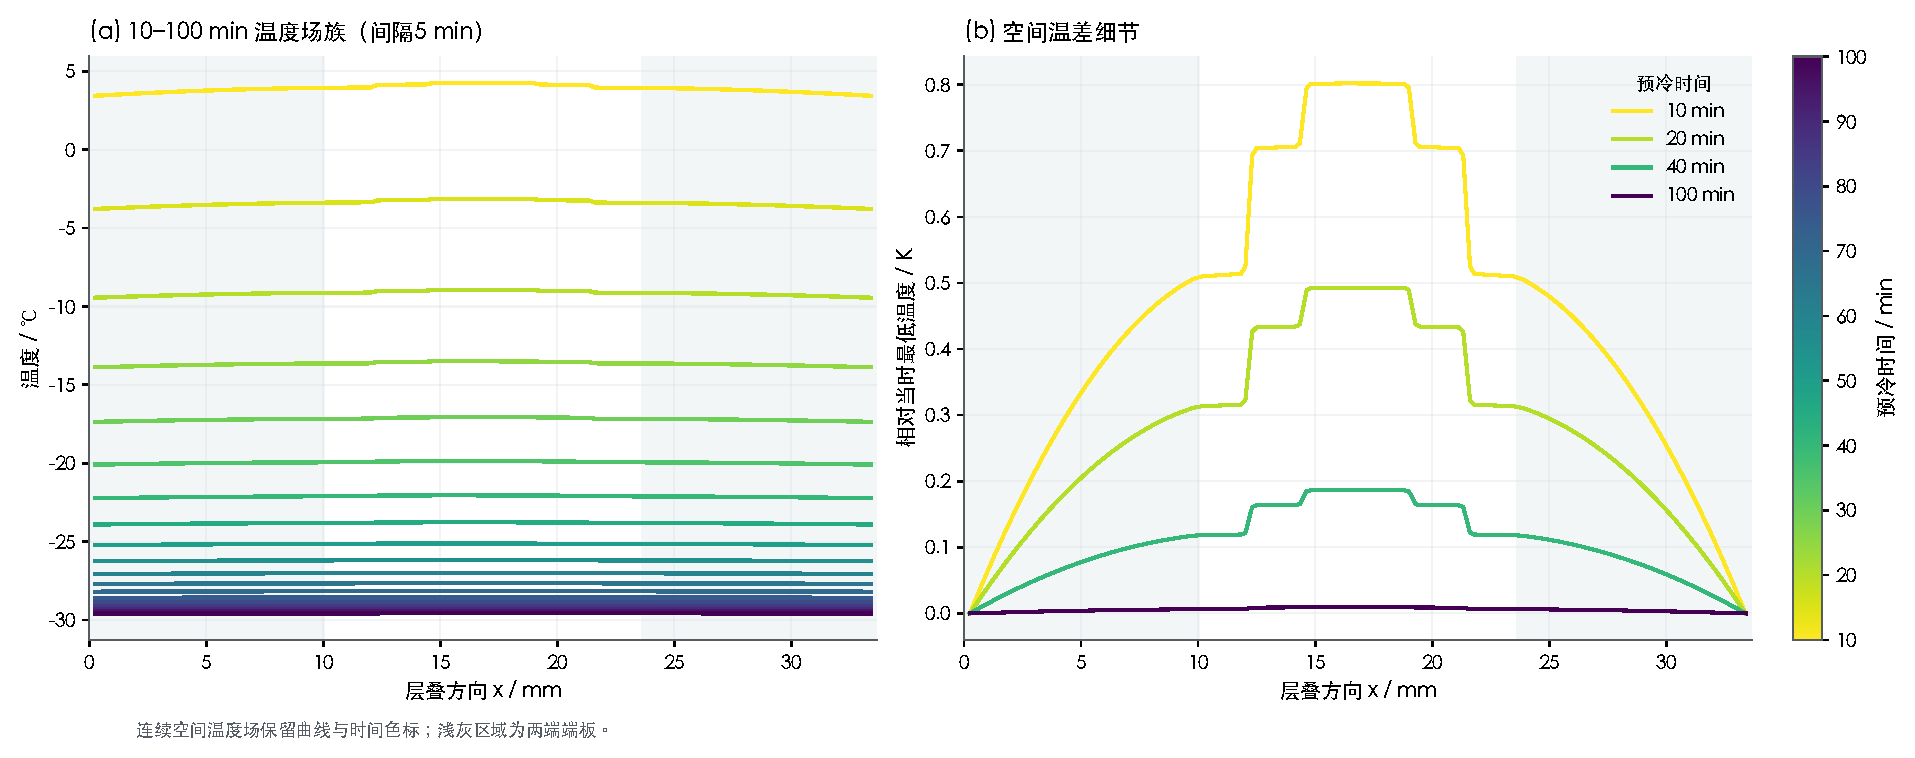
\includegraphics[width=.95\textwidth]{图01_预冷温度场族.pdf}
\caption{不同预冷时间下的整堆温度场及局部温差}
\label{F7-1}
\end{figure}

由图\ref{F7-1}(a)及表\ref{tab:q4:initial}可见，预冷20 min和40 min时温度均呈中部较高、两端较低的分布，但其均温分别约为\(-9.21^\circ\mathrm C\)和\(-22.14^\circ\mathrm C\)，仍明显高于完全冷却工况。端板既承担对外散热，又占据整堆的大部分热容，因此控制了整体降温的主要时间尺度。离散热系统的最慢模态时间常数约为1233.26 s，即20.55 min，与总热容除以两端换热导度所得的集总估算接近。预冷从20 min延长至40 min后，电堆与环境之间的温差继续减小，整堆也逐步接近均匀的\(-30^\circ\mathrm C\)状态。

图\ref{F7-1}(b)将各时刻温度减去相应最低温度后显示局部梯度，可以看到MEA所在薄层的温度变化较集中，而高导热双极板内部温度变化较小。在附件给定物性和端面换热条件下，20 min的全场温差约为0.507 K，40 min时反而减小至0.192 K；对应的五片平均温差仅为0.139 K和0.052 K。因此，两种未完全冷却工况确实存在空间非均匀性，但不能由预冷时间延长直接推出绝对温差增大。本模型给出的主要变化是整体初温进一步降低，初始梯度在较长预冷阶段逐渐衰减。后续启动中若出现数开尔文乃至数十开尔文的片间温差，其主要来源应从端板吸热、分片加热和反应产热的动态竞争中解释。

\subsubsection{动态功率调节与温度、电压及结冰演化}

图\ref{F7-2}--图\ref{F7-4}分别给出三种工况推荐策略的功率、温度、电压和局部冰峰值。各图竖直分界线表示测量保持完成并锁存关热的时刻，阴影部分为关热后60 s的独立观察窗口。因此，评价表\ref{tab:q4:main}中的主结果时应使用分界线之前的数据，而不能把后验段的冰量增长或温度回落混入主窗口极值。

\begin{figure}[!h]
\centering
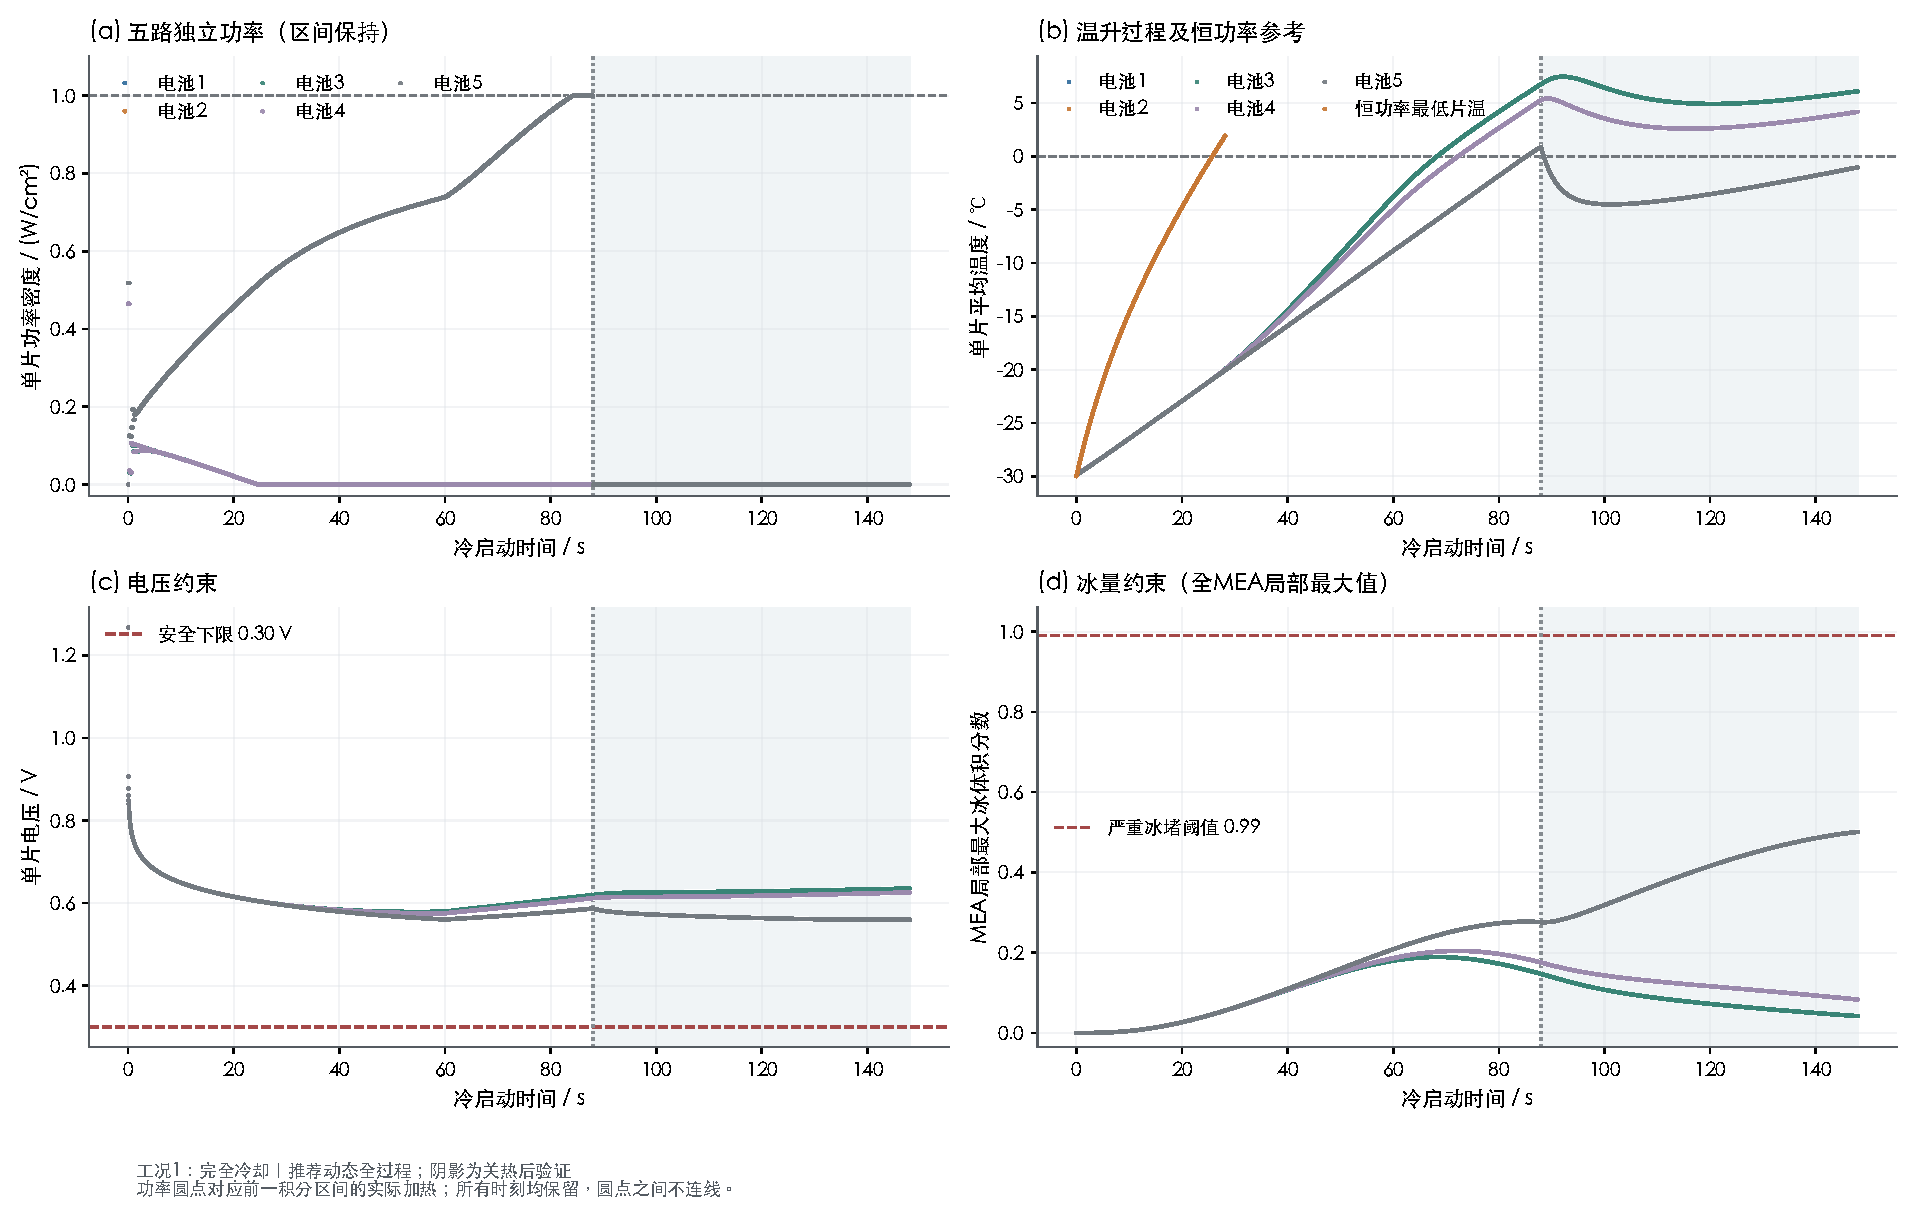
\includegraphics[width=.95\textwidth]{图04_case1_动态控制轨迹.pdf}
\caption{完全冷却工况下推荐动态策略的功率与水热电状态演化}
\label{F7-2}
\end{figure}

对于完全冷却工况，图\ref{F7-2}(a)显示，各片在启动初期均获得短时辅助热输入，随后内部第2--4片的功率逐渐降至零，而端部第1、5片的加热功率随热负荷变化持续增加，后期达到\(1\ \mathrm{W\,cm^{-2}}\)上限。内部电池能够利用自身反应热及片间热传递继续升温，端部电池则同时承担端板吸热与环境散热，因而成为决定全堆首次越过冰点的限制位置。动态控制通过减少内部电池的持续加热，将主要辅助电能集中于端部，使过程最大片间温差控制在6.060 K，显著低于固定恒功率方案的27.003 K。

\begin{figure}[!h]
\centering
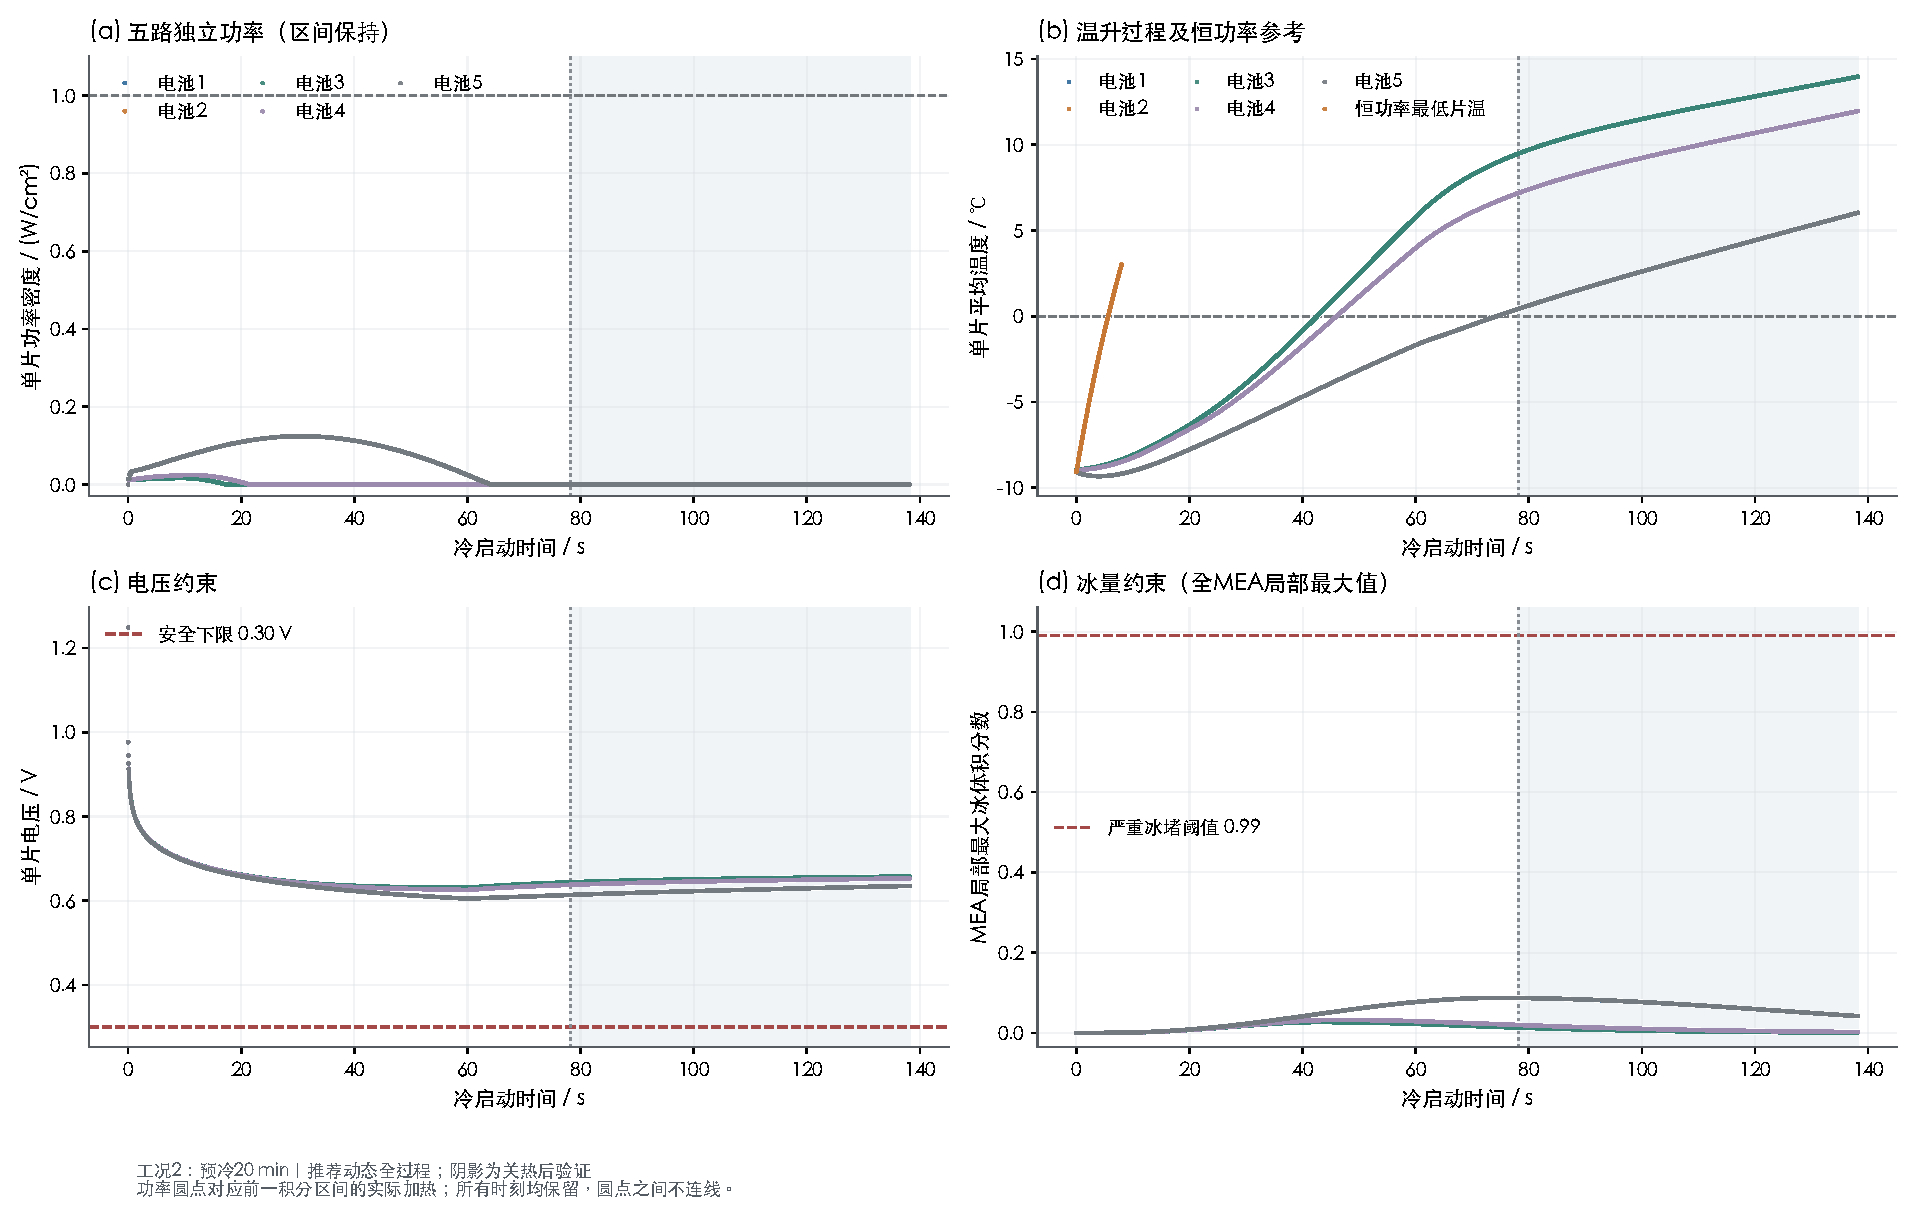
\includegraphics[width=.95\textwidth]{图05_case2_动态控制轨迹.pdf}
\caption{预冷20 min工况下推荐动态策略的功率与水热电状态演化}
\label{F7-3}
\end{figure}

预冷20 min时，各部件仍保留较多显热，辅助加热需求明显减小。由图\ref{F7-3}(a)可见，端部功率先缓慢增加再逐渐回落，峰值仅为\(0.1243\ \mathrm{W\,cm^{-2}}\)，内部各片功率更低。端部电池累计实际加热时间为67.4 s，此后辅助功率已经降至零，而全堆首次达标时刻为74.308 s，测量保持确认时刻为78.2 s。这表明该工况末段主要依靠反应热和已形成的热状态完成升温，控制器无需在整个启动窗口持续供热。端部第1、5片在初期还存在短暂回落，说明较高初温虽然降低了总体热量缺口，但加载初期反应热较弱时，环境散热和端板吸热仍可能超过即时热输入。

\begin{figure}[!h]
\centering
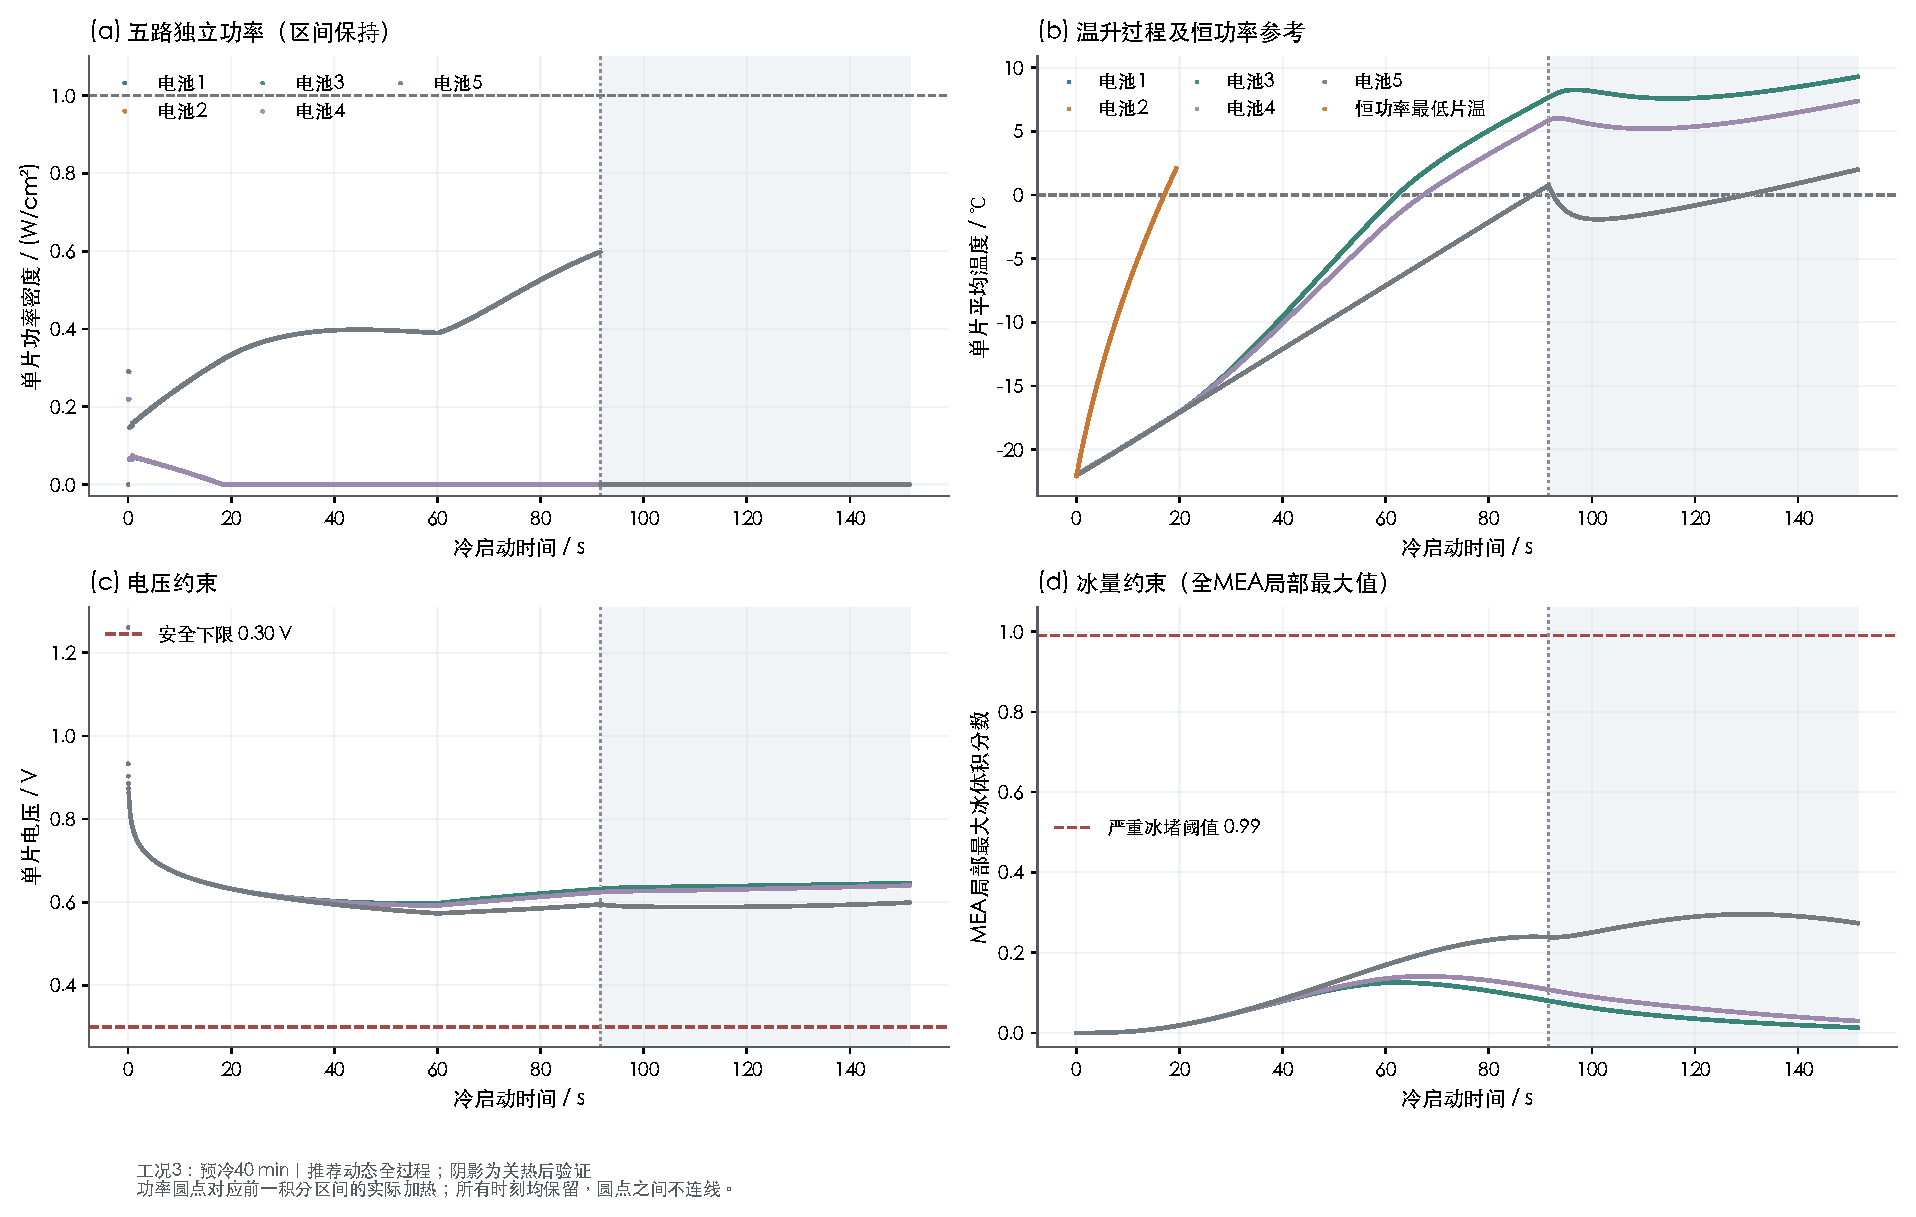
\includegraphics[width=.95\textwidth]{图06_case3_动态控制轨迹.pdf}
\caption{预冷40 min工况下推荐动态策略的功率与水热电状态演化}
\label{F7-4}
\end{figure}

预冷40 min的初温介于前两种工况之间，图\ref{F7-4}(a)所示端部功率总体低于完全冷却工况，峰值约为\(0.5978\ \mathrm{W\,cm^{-2}}\)；内部第2--4片仅在早期加热约18.4 s，端部加热则维持至91.6 s。虽然该工况辅助电能低于完全冷却工况，但其首次启动时间88.539 s略长于完全冷却工况的85.244 s，原因是两种初态分别采用独立整定的控制参数，具有不同的功率水平和参考升温轨迹。因此，跨工况比较时，初温高低能够解释热量需求的变化，却不能脱离控制参数直接判断启动时间的排序。

为了量化空间功率分配，表\ref{tab:q4:cellenergy}给出推荐策略的逐片辅助电能。完全冷却、预冷20 min和预冷40 min工况中，端部两片合计分别占总辅助电能的约96.5\%、91.5\%和97.0\%。与问题三固定策略对第2、4片长期施加满功率不同，动态方案能够根据实际温升及时降低内部片功率，从而减少内部过热。这里的功率分配是片间热耦合与反馈共同作用的结果，并非预先规定只有端部允许加热。

\begin{table}[htbp]
    \centering
    \caption{推荐动态策略的逐片辅助电能分配}
    \vspace{0.3cm}
    \label{tab:q4:cellenergy}
    \renewcommand{\arraystretch}{1.5}
    \begin{tabular}{l c c c c c c}
    \toprule
    \textbf{工况} & \textbf{第1片/J} & \textbf{第2片/J} & \textbf{第3片/J} & \textbf{第4片/J} & \textbf{第5片/J} & \textbf{合计/J}\\
    \midrule
    完全冷却 & 1413.246 & 34.529 & 34.447 & 34.529 & 1413.246 & 2929.996\\
    预冷20 min & 134.347 & 9.674 & 5.566 & 9.674 & 134.348 & 293.609\\
    预冷40 min & 899.927 & 18.566 & 18.399 & 18.566 & 899.927 & 1855.385\\
    \bottomrule
    \end{tabular}
\end{table}

从图\ref{F7-2}--图\ref{F7-4}的电压和冰量子图可见，电流爬升过程中反应产水与低温冻结共同增加冰量，而温度升高和部分区域越过冰点后又促进融冰。推荐策略三工况的最低单片电压分别为0.56044 V、0.60497 V和0.57332 V，局部最大冰体积分数分别为0.277253、0.087293和0.239568，均满足0.30 V和0.99的约束。相比固定恒功率，动态策略在低温区停留更久、累计加载电荷更大，因此主窗口冰峰值更高，最低电压也更低。由此可见，本次优化是在保持安全可行的条件下减少辅助电能，并未同时实现最强的抑冰效果。

还需区分控制结构中设置的安全保护与实际轨迹中触发的动作。状态记录表明，三种推荐方案在无扰动主工况下均未进入安全增强状态，主要控制过程由温升跟踪、温升不足补偿及近目标降功率构成。安全增强提供的是风险上升时的后备规则，不能将其描述为这些主工况节能或抑冰的已发生原因。图中冰量采用全MEA各控制体的局部冰体积分数最大值，与MEA体积平均冰量及孔隙冰饱和度含义不同，后两者不能替代本节的安全约束指标。

\subsubsection{辅助能耗、启动速度与恒功率策略综合比较}

在相同测量保持规则下，定义推荐动态方案相对固定恒功率的辅助节电率为
\begin{equation}
\eta_E=\frac{E_{\rm aux}^{C_H}-E_{\rm aux}^{D_R}}{E_{\rm aux}^{C_H}}\times100\%.
\tag{7-46}\label{eq:q4:saving}
\end{equation}
由表\ref{tab:q4:main}计算得到，完全冷却、预冷20 min和预冷40 min的辅助节电率分别为10.13\%、68.26\%和17.28\%。其中20 min工况初始热量储备较高，沿用完全冷却工况整定的固定大功率会产生较强的加热冗余，动态控制降低功率后的相对收益最大；完全冷却工况需补充的显热较多，端部功率后期达到上限，因此节电空间相对有限。

上述辅助节电伴随着明显的时间代价。固定恒功率三工况的首次启动时间分别为25.741 s、5.606 s和17.037 s，而推荐动态方案分别为85.244 s、74.308 s和88.539 s。推荐方案首次达标时的累计电荷依次为16.573、13.293和17.562\(\ \mathrm{C\,cm^{-2}}\)，虽然均未超过继承的20\(\ \mathrm{C\,cm^{-2}}\)预算，但明显高于固定恒功率的1.657、0.079和0.726\(\ \mathrm{C\,cm^{-2}}\)。更长的反应时间提供了更多反应热，同时也意味着消耗更多反应物。因此，式\eqref{eq:q4:saving}仅衡量电热丝辅助电能的变化，不能直接解释为氢耗或全系统总能耗的同幅下降。

片间一致性也存在工况差异。完全冷却和40 min工况的最大温差分别由27.003 K和19.852 K降至6.060 K和7.243 K，表明动态控制有效抑制了内部片过热；但20 min工况由8.716 K略增至9.054 K。较暖初态允许控制器长时间采用较小辅助功率，端部热损失与内部反应热的不均衡仍会逐步形成温差。因此，动态策略对温差的改善主要体现在本次两个较冷工况，不能概括为所有初态下一致性均优于恒功率。

\begin{figure}[!h]
\centering
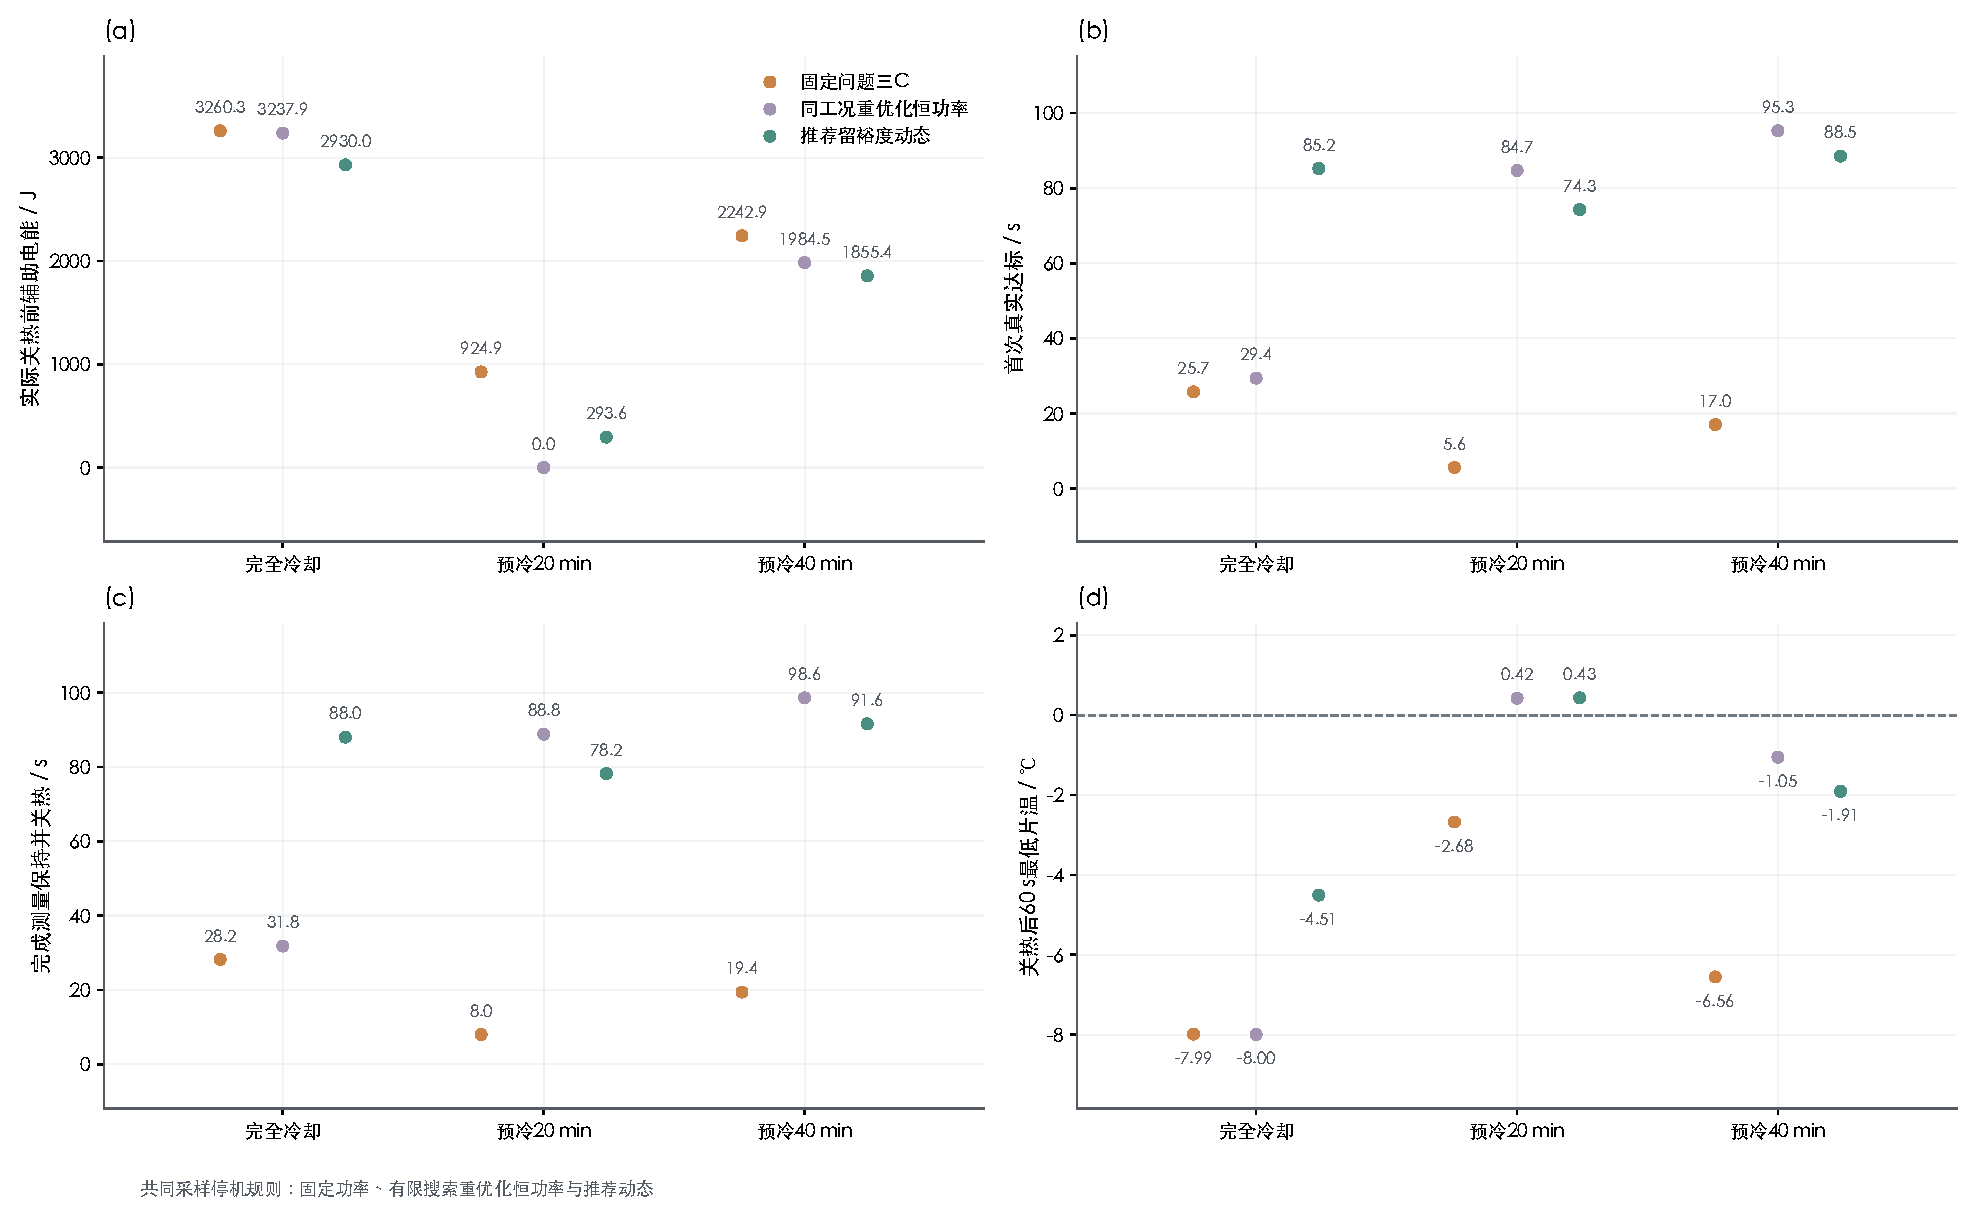
\includegraphics[width=.95\textwidth]{图14_重优化恒功率与推荐动态.pdf}
\caption{固定恒功率、同工况重新优化恒功率与推荐动态策略的比较}
\label{F7-5}
\end{figure}

为进一步区分反馈调节本身的收益与原固定功率分配的适用性，图\ref{F7-5}补充了按各工况重新整定的恒功率方案\(C_*\)。在相同测量停机规则下，\(C_*\)三工况能耗分别为3237.876 J、0 J和1984.470 J，首次启动时间分别为29.416 s、84.725 s和95.287 s。推荐动态方案在完全冷却和40 min工况下相对\(C_*\)分别减少307.880 J和129.085 J，节电约9.51\%和6.50\%；其中40 min工况还将首次启动提前约6.75 s，但完全冷却工况仍需更长时间。

20 min工况的重新优化恒功率退化为五片零加热，名义动态优选方案也得到相同的0 J结果。这说明该初态在给定模型及加载条件下能够利用反应热实现自启动，辅助能耗的非负下界已经达到。推荐方案投入293.609 J，用于缩短启动时间并提高已测试扰动下的可行性，因此不能将其称为该工况的名义最小能耗，也不能将相对原固定功率的全部节电归因于反馈结构独有的优势。重新优化恒功率仅进行了名义参数搜索，其结果也不能代表经过同等扰动整定后的恒功率能力上限。

此外，本章固定功率的首次达标复算能耗约为2976.015 J，而采用测量保持规则后增至3260.281 J。前者与第六章约2975.3 J的结果接近，微小差异与数值设置及事件求解精度有关；后者增加的能耗主要来自温度裕度确认与保持期间继续加热。因此，本章节电率始终使用表\ref{tab:q4:main}中的共同停机基准，避免将第六章首次达标能耗与本章实际关热能耗直接相除。

\subsubsection{预冷时间对恒功率冷启动及单片一致性的影响}

针对问题四第（2）小问，将预冷时间依次取为10、15、\(\ldots\)、100 min，并始终施加问题三的固定功率分配和统一电流曲线。该组计算用于隔离预冷程度的影响，采用首次真实达标即结束的口径，不附加测量温度裕度和2 s保持。图\ref{F7-6}给出全部19个扫描点，表\ref{tab:q4:scan}选取其中六个代表时刻列出结果。

\begin{figure}[!h]
\centering
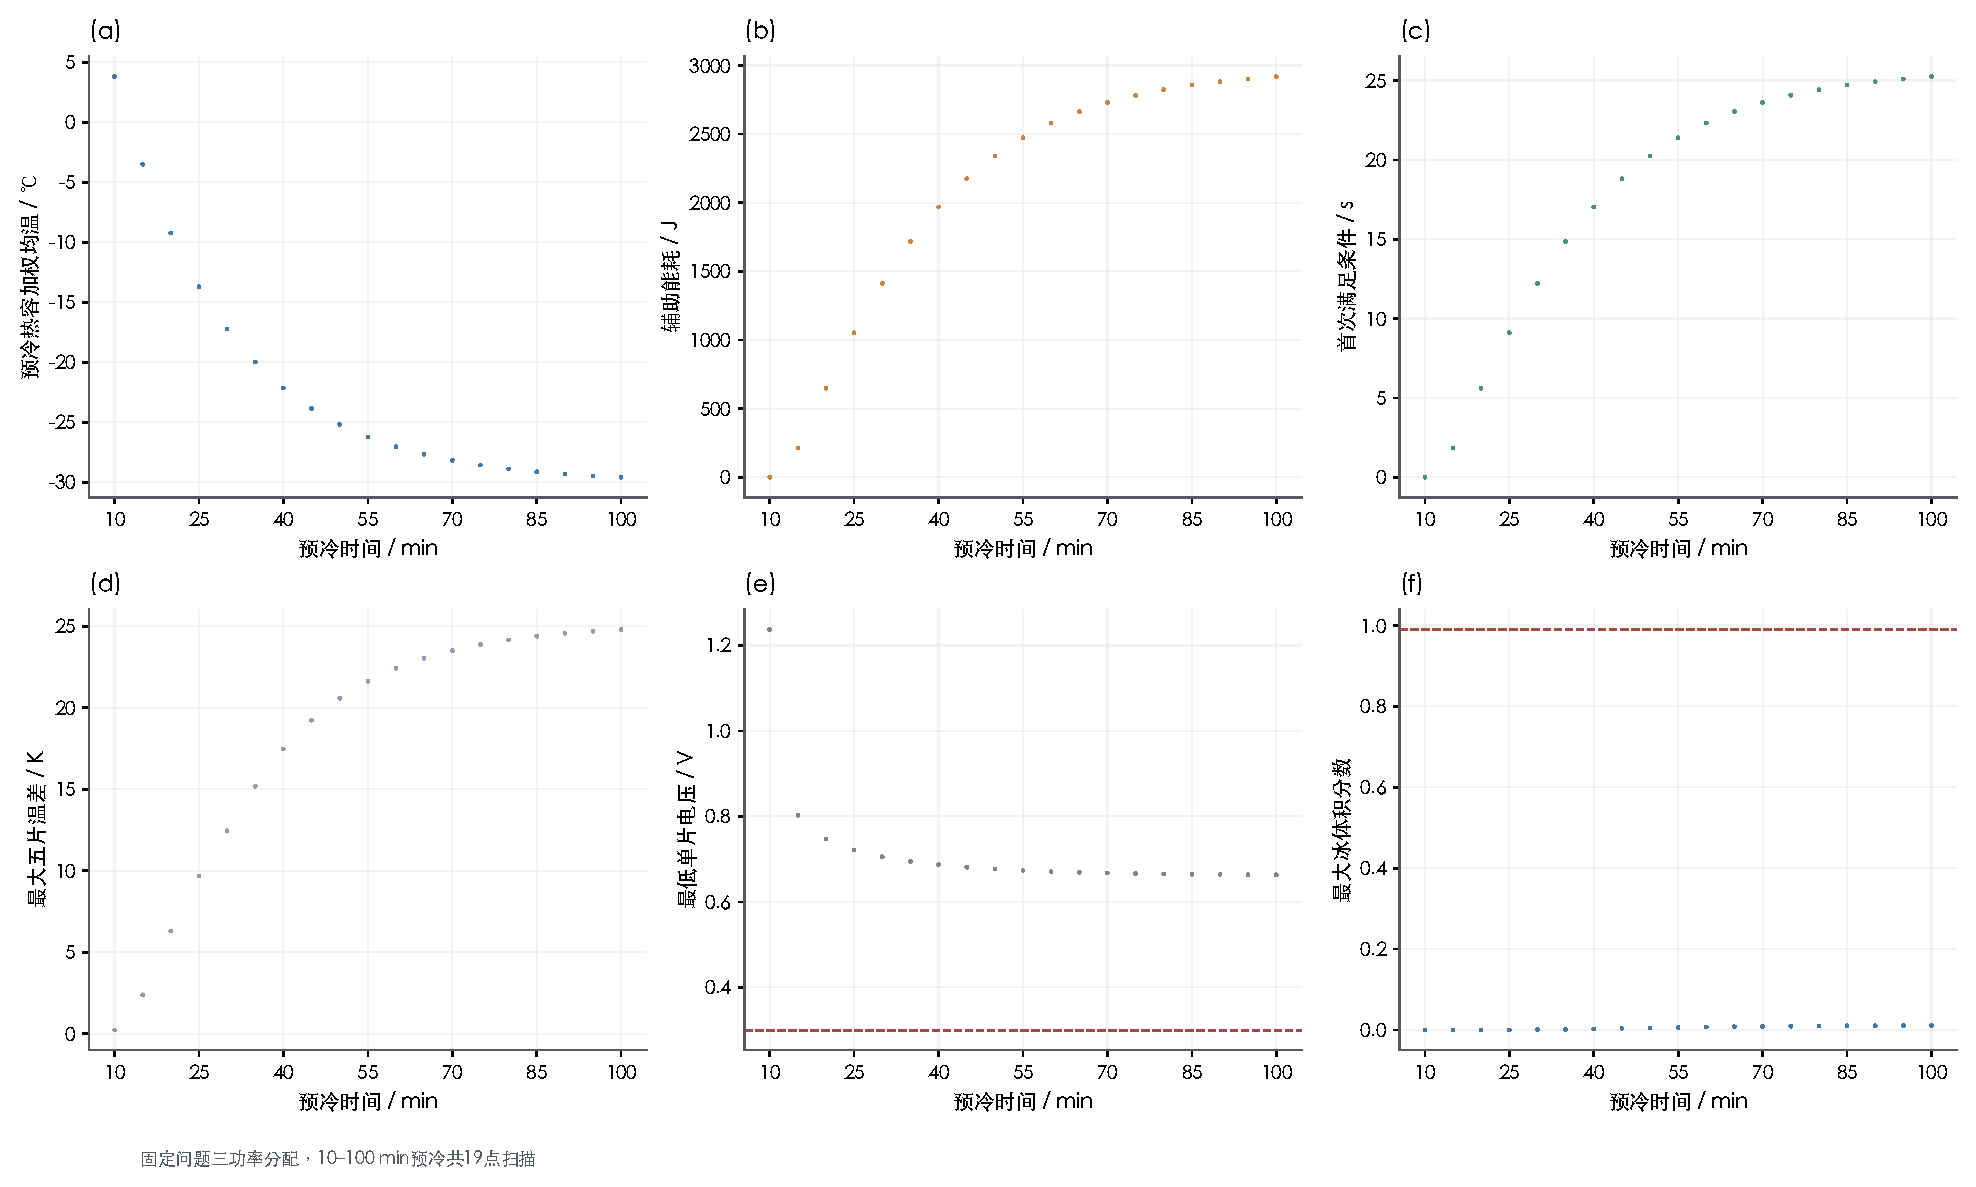
\includegraphics[width=.95\textwidth]{图08_预冷时间扫描.pdf}
\caption{预冷时间对固定恒功率启动性能的影响}
\label{F7-6}
\end{figure}

\begin{table}[htbp]
    \centering
    \caption{不同预冷时间下固定恒功率启动的代表性结果}
    \vspace{0.3cm}
    \label{tab:q4:scan}
    \renewcommand{\arraystretch}{1.5}
    \resizebox{\textwidth}{!}{
    \begin{tabular}{c c c c c c c c}
    \toprule
    \shortstack{\textbf{预冷时间}\\\(/\mathrm{min}\)} & \shortstack{\textbf{热容加权初温}\\\(/{}^\circ\mathrm C\)} & \shortstack{\textbf{首次达标}\\\(/\mathrm s\)} & \shortstack{\textbf{辅助电能}\\\(/\mathrm J\)} & \shortstack{\textbf{最大五片温差}\\\(/\mathrm K\)} & \shortstack{\textbf{最低电压}\\\(/\mathrm V\)} & \shortstack{\textbf{最大局部}\\\textbf{冰体积分数}} & \textbf{结果}\\
    \midrule
    10 & 3.812 & 0 & 0 & 0.225 & 1.23732 & 0 & 初态已达标\\
    20 & -9.212 & 5.606 & 648.136 & 6.298 & 0.74738 & \(9.528\times10^{-5}\) & 成功\\
    40 & -22.143 & 17.037 & 1969.681 & 17.469 & 0.68684 & 0.002818 & 成功\\
    60 & -27.030 & 22.316 & 2579.978 & 22.416 & 0.67089 & 0.007411 & 成功\\
    80 & -28.878 & 24.428 & 2824.169 & 24.161 & 0.66534 & 0.010141 & 成功\\
    100 & -29.576 & 25.242 & 2918.317 & 24.799 & 0.66329 & 0.011347 & 成功\\
    \bottomrule
    \end{tabular}}
\end{table}

由图\ref{F7-6}(a)--(c)可见，预冷越充分，整堆初温越接近\(-30^\circ\mathrm C\)，固定功率启动所需时间和辅助电能也随之增加，但增加幅度逐渐减小。10 min时五片初温约为4.01--4.24\(^\circ\mathrm C\)，起始状态已经满足温度条件，因此首次达标时间和辅助能耗均为零；该点不代表经历了一个零时间的加热过程，也不构成任意后续负载下可持续运行的证明。20 min和40 min的辅助电能分别为648.136 J和1969.681 J，而100 min时达到2918.317 J，逐步接近完全冷却工况约2976.015 J的首次达标基准。由于所有扫描点的总加热功率保持不变，能耗增长与首次启动时间延长直接对应，其根源是预冷后需要补充的显热增加。

图\ref{F7-1}与图\ref{F7-6}(d)还揭示了初始温差和启动温差的不同变化方向。随着预冷时间由10 min增加到100 min，完整预冷场的绝对温差由约0.825 K减至0.010 K，五片初始均温差由约0.225 K减至0.003 K；但启动过程最大片间温差却由0.225 K增加至24.799 K。较深预冷使大热容端板处于更低温度，启动时端部电池需要持续向端板供热，而内部电池在固定加热和反应产热共同作用下较快升温。因而，较均匀的低温初态并不意味着较均匀的启动过程，启动期间重新形成的端部热负荷差异才是后期片间不一致性的主要原因。

在电压与冰量方面，预冷时间增加使低温产水持续时间延长，局部冰峰值逐渐升高，最低单片电压逐渐降低。即使预冷100 min，最低电压仍为0.66329 V，局部冰峰值仅为0.011347，均保持在规定阈值内。全部19个离散预冷时间点均完成首次启动，说明问题三固定功率方案在所考察区间内具有可行性；本次扫描没有发现失败点，因此不能据此给出未经识别的临界预冷时间。该结论仅针对已计算的19个点及固定参数条件。

\subsubsection{关热后温度回落与持续运行特性}

首次越过冰点并完成短时保持，只说明启动阶段满足规定判据，并不等价于整个电堆已经具备维持暖态的热储备。为检验这一差异，在各方案实际关热后继续按题给电流曲线运行60 s，辅助功率保持锁存为零。表\ref{tab:q4:post}给出推荐方案关热时的状态及后验段极值，同时列出固定恒功率方案的后验最低温度作为参照。

\begin{table}[htbp]
    \centering
    \caption{推荐动态策略关热状态及关热后60 s的运行结果}
    \vspace{0.3cm}
    \label{tab:q4:post}
    \renewcommand{\arraystretch}{1.5}
    \resizebox{\textwidth}{!}{
    \begin{tabular}{l c c c c c c}
    \toprule
    \textbf{工况} & \shortstack{\textbf{关热最低片温}\\\(/{}^\circ\mathrm C\)} & \shortstack{\textbf{关热左端板温度}\\\(/{}^\circ\mathrm C\)} & \shortstack{\textbf{后验最低片温}\\\(/{}^\circ\mathrm C\)} & \shortstack{\textbf{后验最低电压}\\\(/\mathrm V\)} & \shortstack{\textbf{后验局部}\\\textbf{冰峰值}} & \shortstack{\(C_H\)\textbf{后验最低片温}\\\(/{}^\circ\mathrm C\)}\\
    \midrule
    完全冷却 & 0.882 & -14.471 & -4.508 & 0.55967 & 0.50104 & -7.986\\
    预冷20 min & 0.433 & -5.115 & 0.433 & 0.61376 & 0.08702 & -2.677\\
    预冷40 min & 0.763 & -10.288 & -1.910 & 0.58853 & 0.29566 & -6.556\\
    \bottomrule
    \end{tabular}}
\end{table}

由表\ref{tab:q4:post}及图\ref{F7-2}、图\ref{F7-4}的阴影部分可见，完全冷却和40 min工况虽然在关热时全部单电池均已高于冰点，但端板仍分别约为\(-14.47^\circ\mathrm C\)和\(-10.29^\circ\mathrm C\)。辅助热源一旦撤去，端板继续从端部单电池吸热，使最低片温分别降至\(-4.508^\circ\mathrm C\)和\(-1.910^\circ\mathrm C\)。这与第六章发现的端板热惯性效应一致，说明仅根据单电池温度过零及2 s保持，尚不能判定端板热汇已经充分减弱。

相比之下，20 min工况的初始热储备更高，且在正式关热之前辅助功率已提前降至零，反应热能够维持其继续升温；关热后最低片温保持在0.433\(^\circ\mathrm C\)以上。完全冷却和40 min工况虽再次进入零下区间，但后验最低电压仍高于0.30 V，冰峰值也未达到0.99，因此应表述为未维持持续暖态，而不是将其与电压失效或严重冰堵混为一谈。与固定恒功率方案相比，推荐动态方案在本次60 s观察窗口内减轻了回冷，但仍未在全部工况消除该现象。

上述后验段不计入主表辅助电能，且不允许重新开启加热。若进一步要求关热后始终保持冰点以上，则需将这一要求明确纳入优化约束，并重新整定功率与热裕度；本次结果不能直接外推为已满足该更强目标。后验段继续加载也会消耗反应物，其作用是检验延续运行状态，不能混入首次启动的电荷预算。

\subsubsection{参数灵敏度与控制策略稳健性分析}

图\ref{F7-7}分别展示预冷传热参数变化和名义动态控制参数扰动的影响。预冷部分同时考察绝对温差及其相对于整堆平均超温的比值，以区分内部传热不均匀程度与整体冷却速度；启动部分则固定名义控制结构，对片间导度、端板耦合导度、环境换热及控制参数逐项扰动。

\begin{figure}[!h]
\centering
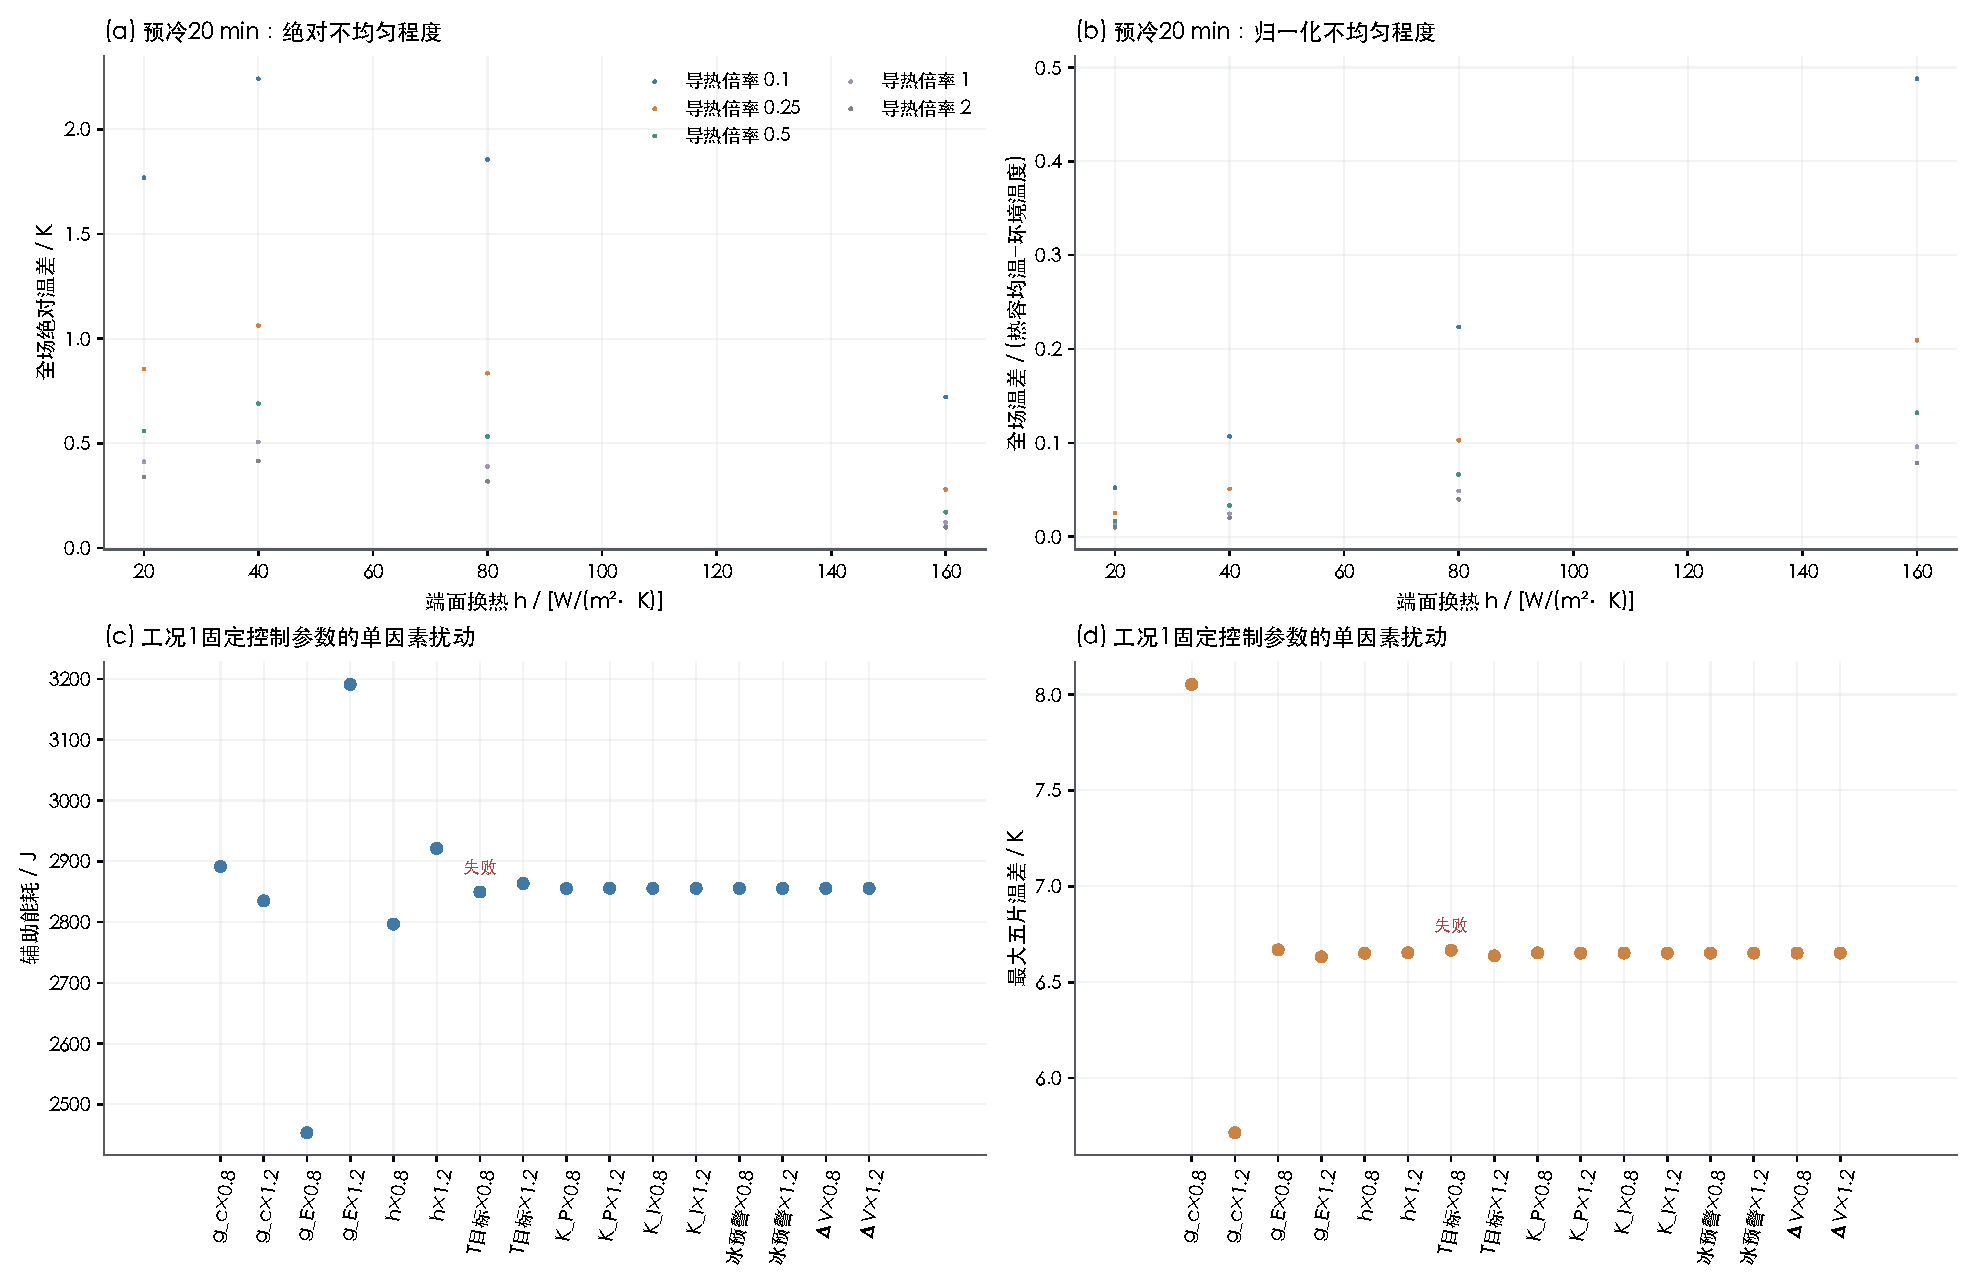
\includegraphics[width=.95\textwidth]{图11_物理参数与控制器敏感性.pdf}
\caption{预冷传热参数与名义动态控制参数的敏感性}
\label{F7-7}
\end{figure}

由图\ref{F7-7}(a)、(b)可见，内部导热能力降低时，端部与中部更难迅速交换热量，预冷温度场的相对非均匀程度增大。端面换热增强则同时提高外部散热强度并加快整体降温，因此固定预冷时刻的绝对温差不一定随换热系数单调增加；当电堆已经较接近环境温度时，可用于维持空间梯度的超温也随之减小。采用温差与热容加权均温超出环境温度之比，可更清楚地识别外部换热与内部导热竞争的影响。

启动敏感性表明，端板耦合导度对辅助电能的影响较突出。以完全冷却的名义方案为例，将端板耦合导度降低20\%后，辅助电能约降至2453.251 J；提高20\%后则增至约3190.957 J，显著偏离基准2855.408 J。端板耦合越强，启动过程中单电池向低温端板传递的热量越多，维持参考温升所需的辅助电能也越高。另一方面，个别控制参数扰动会导致未能完成测量保持停机，故图中的失败候选即使已消耗较少电能，也不能作为更优的成功方案。图\ref{F7-7}使用名义动态参数，其作用是揭示影响机制，不代表推荐方案已经在全部参数组合中得到严格鲁棒保证。

\begin{figure}[!h]
\centering
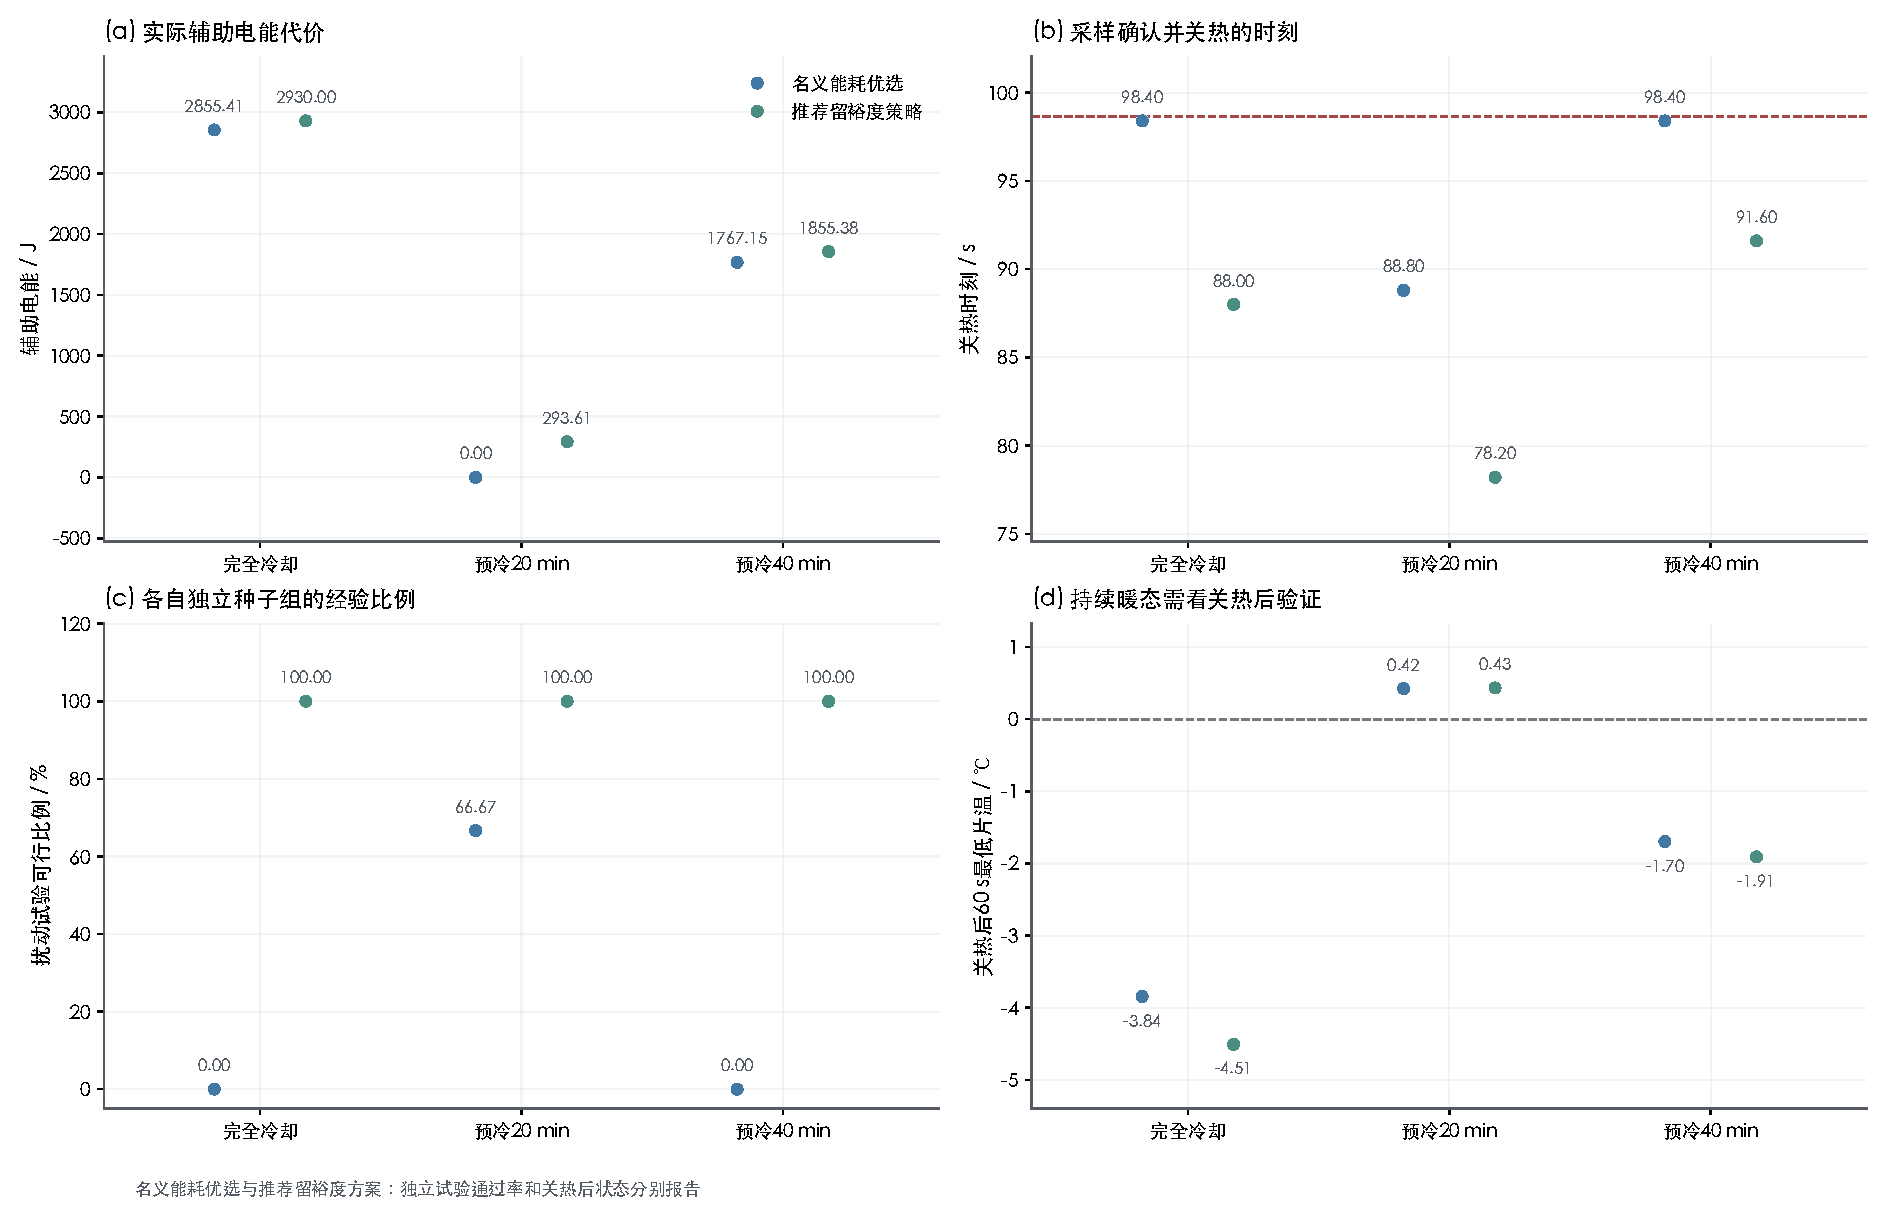
\includegraphics[width=.95\textwidth]{图13_名义与留裕度备选.pdf}
\caption{名义节能方案与推荐留裕度方案的能耗、时间及扰动表现}
\label{F7-8}
\end{figure}

由图\ref{F7-8}(a)、(b)可见，名义方案\(D_N\)三工况辅助电能为2855.408 J、0 J和1767.146 J，其中两个较冷工况的实际关热时刻均达到98.4 s，靠近允许的保持窗口上限。推荐方案\(D_R\)分别增加约74.588 J、293.609 J和88.239 J，将关热时刻提前至88.0 s、78.2 s和91.6 s。其目的在于为初温偏差、滤波滞后及物性失配保留可用余量，而不是在名义模型下进一步压低辅助能耗。

名义方案在原测量噪声与初场偏差试验中，仅20/90次满足全部可行性条件，成功样本集中于20 min工况；推荐方案在参数冻结后的独立噪声与初场试验中通过90/90次，并在24个物性失配与噪声联合场景中全部通过。两组噪声试验采用不同随机种子，因而这些比例可以说明各方案在所列场景下的表现，但不能作为严格配对的统计优势证明。固定恒功率\(C_H\)在相同最终验证场景下也全部通过，说明它本身具有较充分的启动时间余量。推荐动态方案的价值在于在这些已验证场景中保留可行性的同时降低辅助电能，而不是声称只有动态控制才能抵御扰动。

\begin{figure}[!h]
\centering
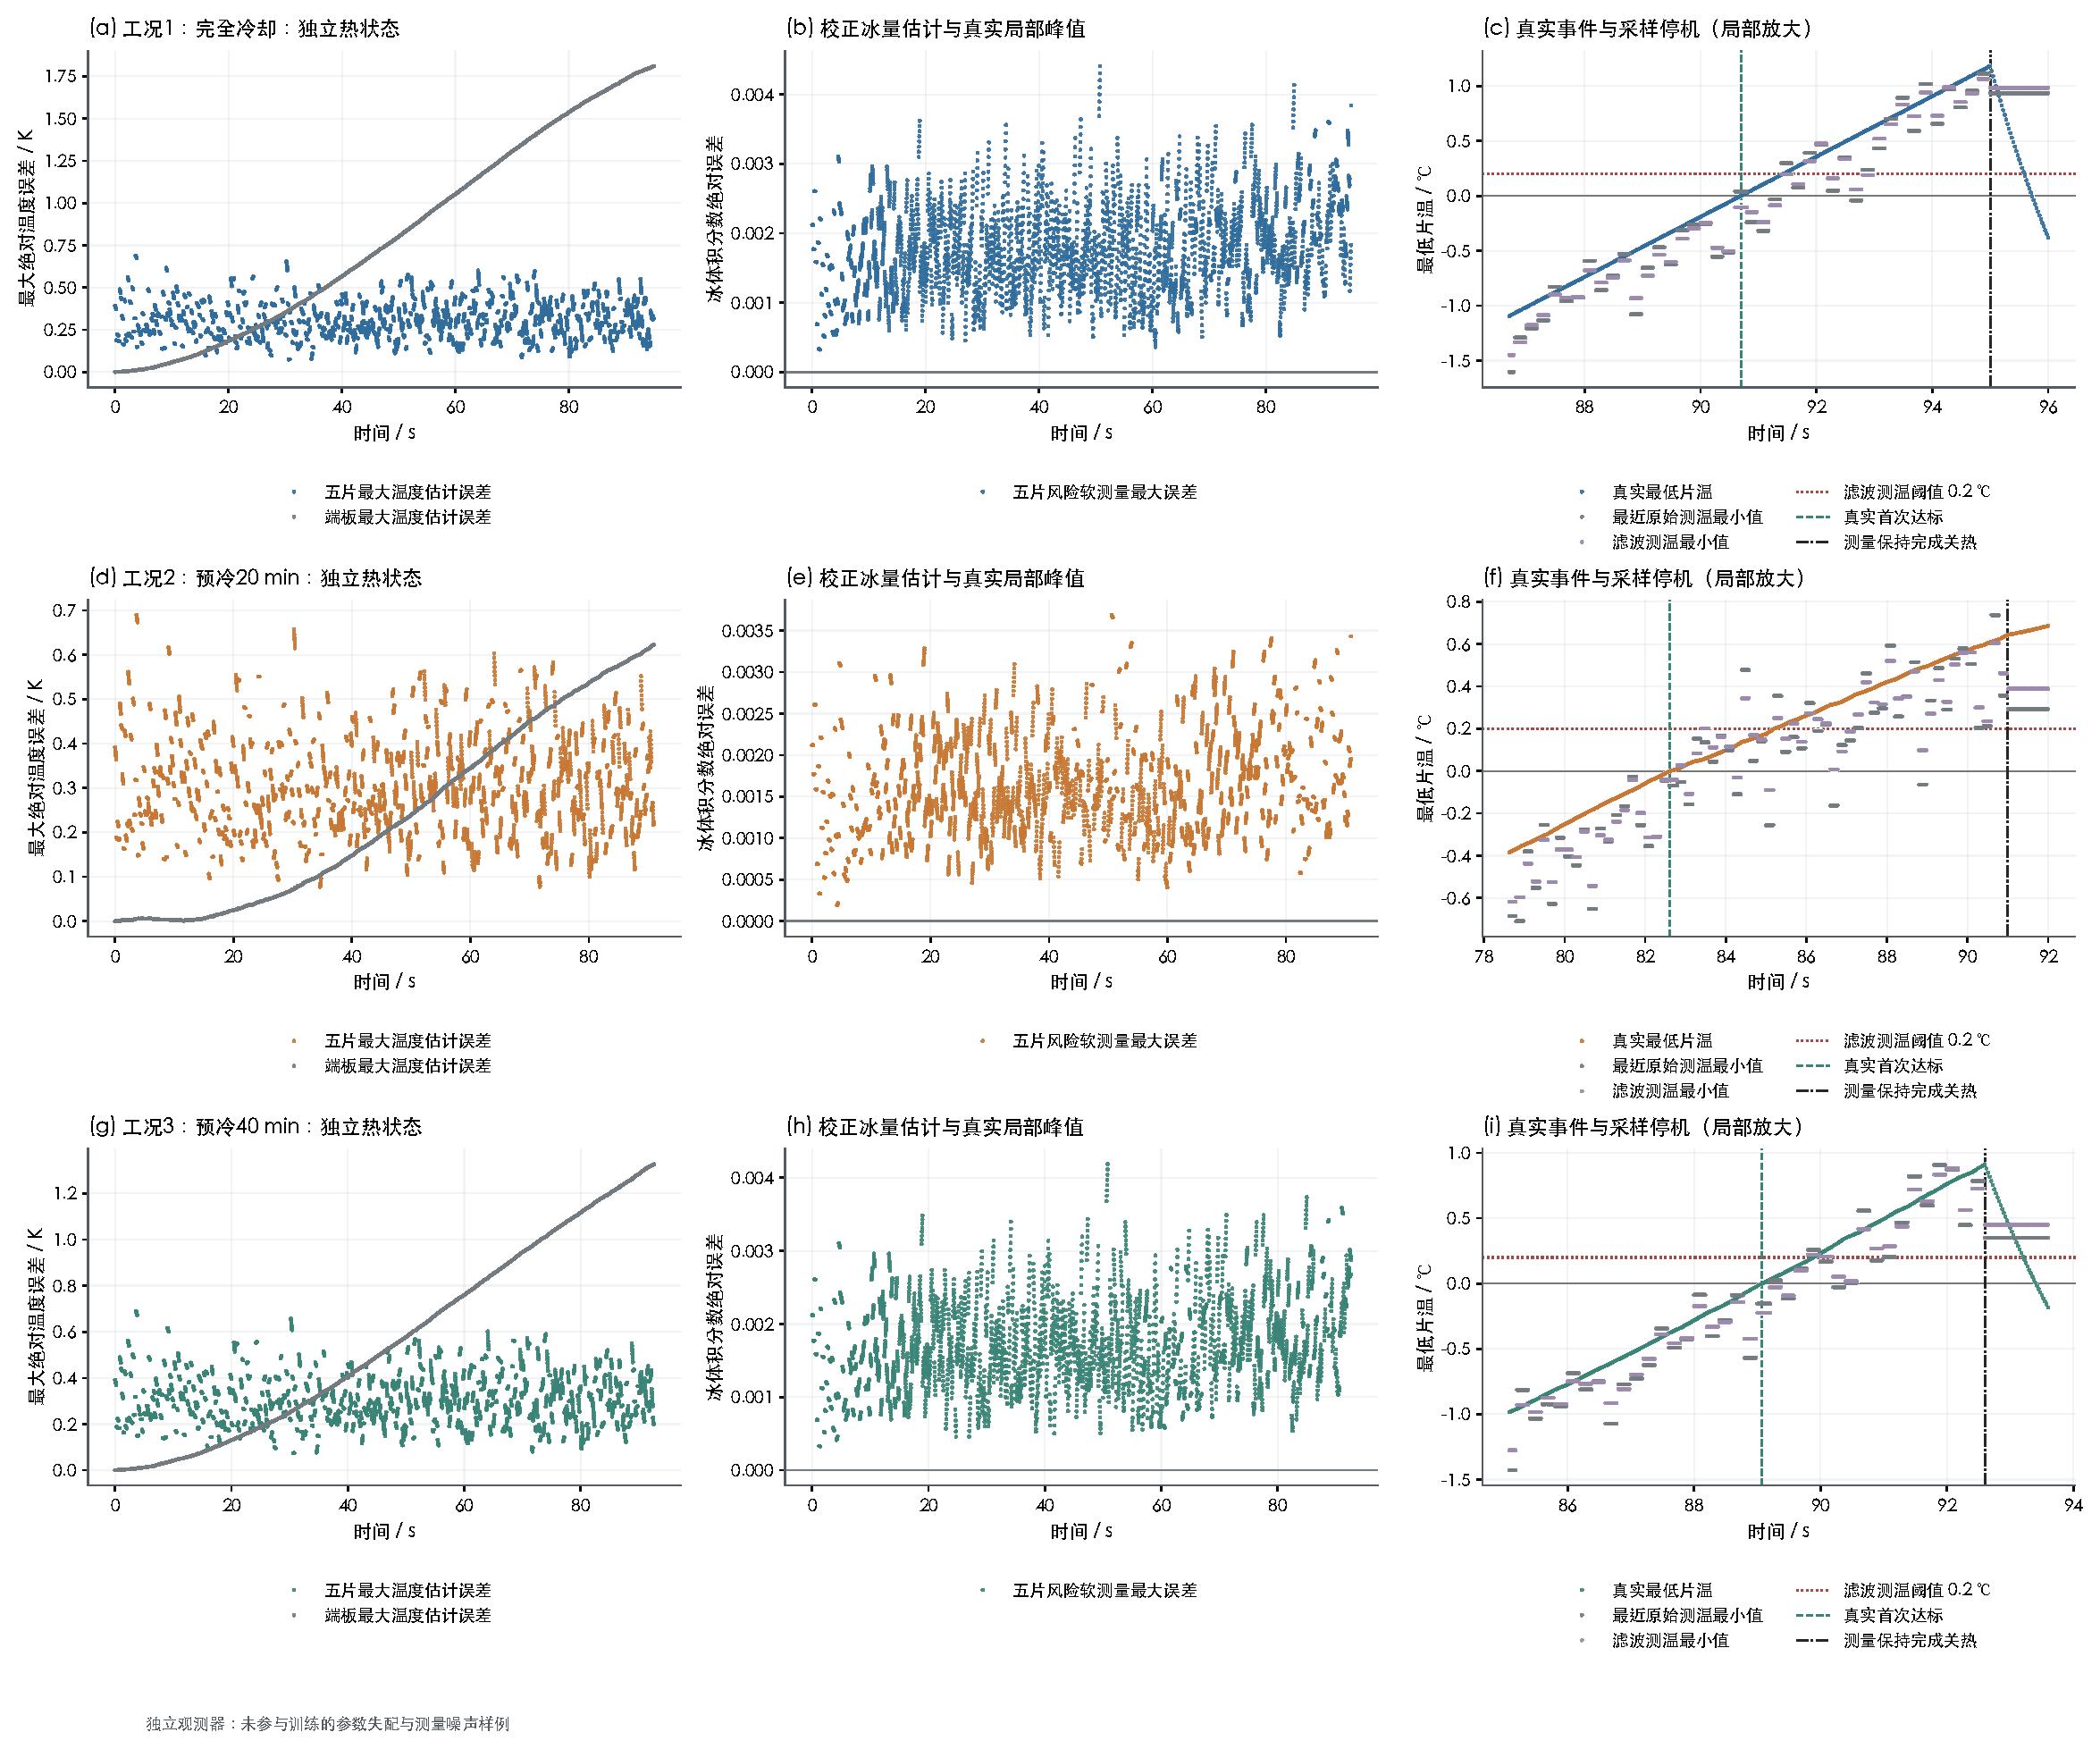
\includegraphics[width=.95\textwidth]{图16_观测器误差与测量停机.pdf}
\caption{参数失配与测量噪声下的观测误差及停机事件辨析}
\label{F7-9}
\end{figure}

图\ref{F7-9}进一步检验反馈信息的可获得性。图中采用未参与训练的参数失配与测量噪声样例，控制器仅使用独立观测模型和温度、电压采样。端板温度估计随物性失配出现偏差，说明观测状态并未直接复制被控对象的真实状态；冰风险估计与真实局部冰峰值之间也保留误差，不能视为对完整冰场的精确重构。以图\ref{F7-9}(c)的完全冷却样例为例，真实首次达标约为90.70 s，而滤波测温满足温度裕度并连续保持后，到95.0 s才确认关热；20 min样例的相应时刻约为82.61 s和91.0 s。这种差异来自传感采样、滤波和保持计时，说明实际关热时刻不能简单设为\(t_s+2\ \mathrm s\)。

因此，推荐方案的稳健性应由真实状态下的成功时刻、路径约束和关热前真实状态连续保持是否完成共同判定，不能仅以测量判据被触发为依据。图\ref{F7-8}(d)仍显示部分工况关热后回冷，也再次说明本节的扰动可行性验证与持续暖态验证属于不同层次。

\subsubsection{能量守恒、数值收敛与结果可靠性分析}

为解释节电的能量来源，将启动主窗口中的辅助加热、反应产热、相变净释热、环境散热和离散显热增量分别累计。按照与时间推进相同的热容和时间积分定义，离散能量残差写为
\begin{equation}
R_E=E_{\rm aux}+E_{\rm gen}+E_{\rm phase}-E_{\rm loss}-E_{\rm sensible}.
\tag{7-47}\label{eq:q4:energyresidual}
\end{equation}
其中\(E_{\rm phase}\)为带符号的相变净热，\(E_{\rm sensible}\)按各时间步使用的有效热容与温度增量累计。该量与离散方程保持一致，不将随含水状态变化的有效热容简单替换为一个常数乘总温升。

\begin{figure}[!h]
\centering
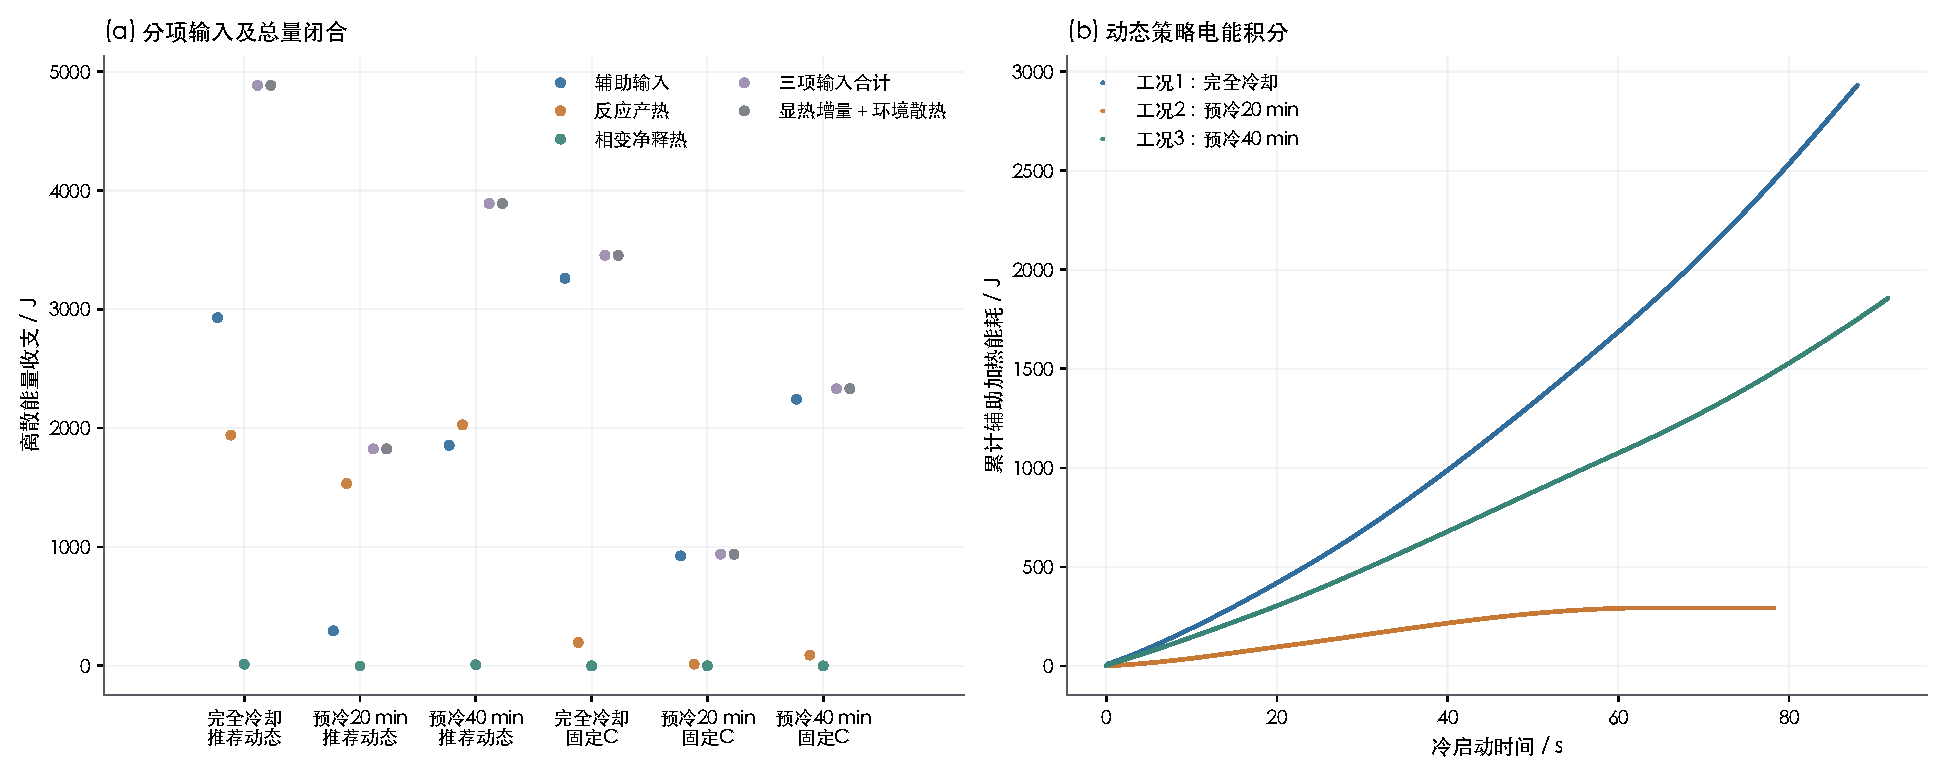
\includegraphics[width=.95\textwidth]{图09_能量收支与累积能耗.pdf}
\caption{推荐动态与固定恒功率策略的能量收支及累计辅助电能}
\label{F7-10}
\end{figure}

由图\ref{F7-10}(a)可见，各工况热输入总量与显热增量、环境散热之和相互吻合。完全冷却推荐方案在关热前输入辅助热2929.996 J、反应热1941.572 J和相变净热13.454 J，扣除环境散热272.961 J后，离散显热增量为4612.062 J。相同工况固定恒功率方案的反应热仅为194.959 J，而辅助输入为3260.281 J。因此，动态方案虽然延长了升温过程并增加环境散热，却通过更充分地利用反应热降低了所需辅助电能，同时使关热时端板温度较高。这也解释了其关热后回冷较固定策略有所减轻。

对于预冷20 min工况，推荐方案的反应热达到1533.862 J，明显高于293.609 J的辅助热；相变净热为\(-2.020\) J，环境散热为394.056 J，最终显热增量约为1431.395 J。预冷40 min时，辅助热和反应热分别为1855.385 J与2027.484 J，二者共同提供主要升温能量。图\ref{F7-10}(b)中，20 min工况累计辅助电能在末段转为水平，而其余两种工况仍随端部加热持续增加，与前述功率轨迹及提前停止实际加热的现象一致。

三工况推荐策略的离散能量残差绝对值约为\(10^{-11}\)--\(10^{-10}\) J，完整轨迹水量残差最大绝对值约为\(10^{-16}\)--\(10^{-15}\) kg，表明当前离散更新中的收支能够闭合。预冷阶段另行检查全堆内能减少与两端累计散热的一致性，并利用同网格矩阵指数解校验时间离散。守恒残差很小主要说明数值收支自洽，仍需结合独立参考和网格加密判断离散误差，不能单凭该残差推断物理预测没有误差。

\begin{figure}[!h]
\centering
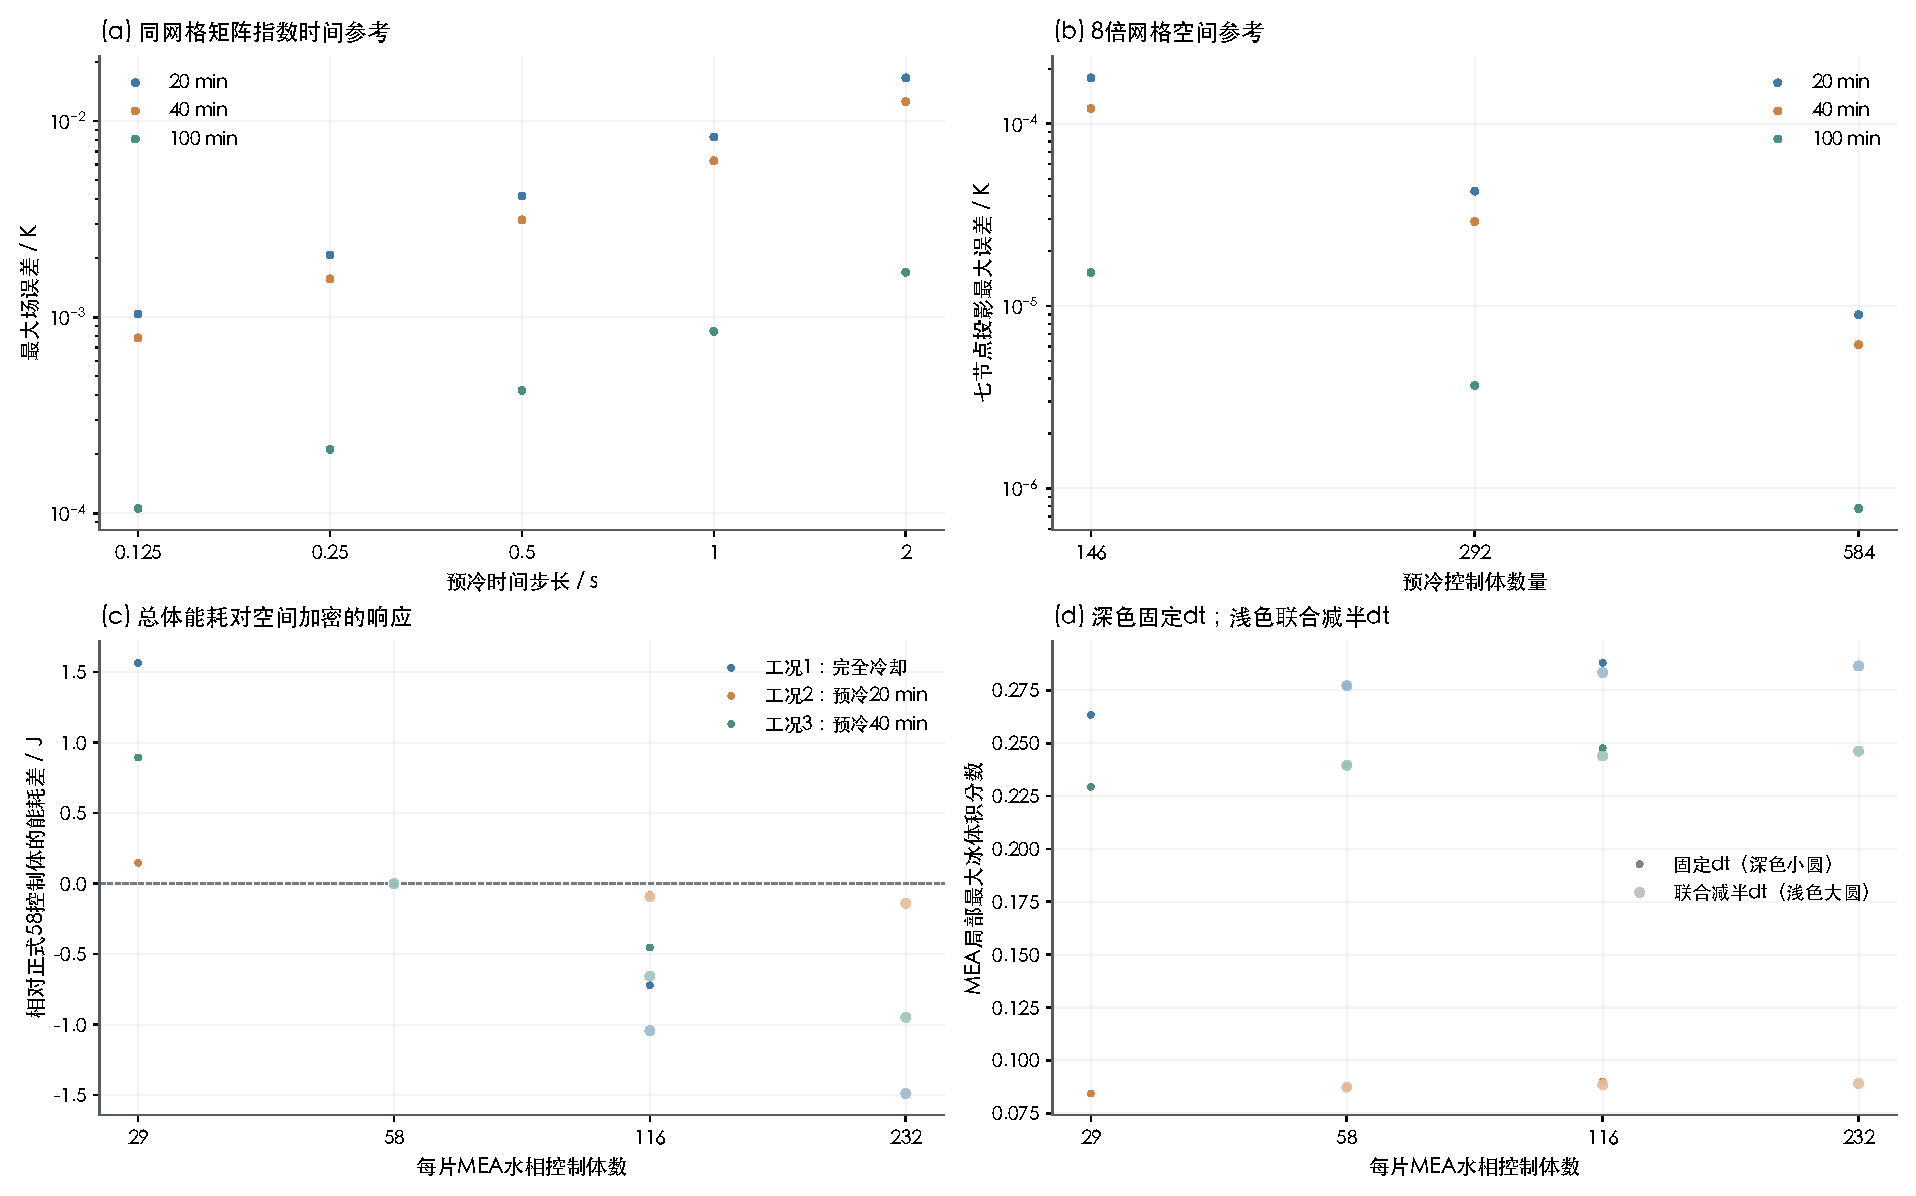
\includegraphics[width=.95\textwidth]{图10_网格步长与控制周期检验.pdf}
\caption{预冷温度场与推荐动态启动结果的时间和空间收敛检验}
\label{F7-11}
\end{figure}

由图\ref{F7-11}(a)、(b)可见，预冷时间步从2 s减小至0.25 s时，20 min温度场相对同网格矩阵指数解的最大误差由约0.0166 K降至0.00208 K，继续减小至0.125 s后约为0.00104 K，表现出后向欧拉方法预期的收敛趋势。增加空间控制体数量后，七节点投影相对加密参考的误差也进一步下降，说明预冷初始场的离散精度能够满足三工况差异分析的需要。

对启动过程，固定正式控制参数和0.2 s采样周期，将每片水相控制体由58个加密至232个，同时把时间步从0.025 s减小至0.00625 s。三工况辅助电能分别由2929.996 J、293.609 J和1855.385 J变为2928.508 J、293.469 J和1854.436 J，相对变化均约为0.05\%；首次启动时间变化均小于0.008 s，实际关热时刻保持不变。图\ref{F7-11}(c)由此表明，主要能耗和时间结论对进一步联合加密较稳定。

图\ref{F7-11}(d)同时显示，局部冰峰值比总能耗更依赖空间分辨率。完全冷却工况由0.27725升至0.28658，20 min工况由0.08729升至0.08912，40 min工况由0.23957升至0.24623。尽管加密后的冰量仍远低于0.99约束，且不改变三工况的可行性判断，但其相对变化大于辅助电能的变化，因此不能将所有局部状态均描述为完全网格无关。综合基准复现、守恒检查、独立参考、离散加密与扰动验证，本章结果可支持给定模型及搜索范围内的性能比较；预冷和启动阶段沿用的有效物性、换热位置近似，以及尚缺新增实验校准的限制仍需保留。

\subsection{问题四小结}

针对不同预冷程度下电堆动态辅助启动问题，本文在前述水--冰--热--电耦合模型基础上，建立了整堆预冷传热模型，将预冷温度场映射为五片电池与两端端板的非均匀初态；进一步利用温度、电压及其变化率构造状态识别与独立观测器，通过前馈、PI反馈、温升不足补偿、安全增强和测量保持停机形成分片动态加热策略。以辅助电能为首要目标完成有限参数搜索后，再根据扰动训练场景选择留有温度和时间裕度的推荐方案。

结果表明，推荐方案在完全冷却、预冷20 min和预冷40 min工况下分别消耗2929.996 J、293.609 J和1855.385 J辅助电能，相对共同测量停机规则下的问题三固定功率方案节电10.13\%、68.26\%和17.28\%。其节能主要来自减少内部片持续加热，并利用较长启动过程中的反应热分担升温需求，代价是启动较慢且主窗口结冰水平较高；三工况电压、冰量及启动电荷仍满足约束。推荐方案通过所列独立扰动场景，但完全冷却与40 min工况关热后仍出现回冷，因此完成首次启动及短时保持并不等同于实现持续暖态。

在10--100 min预冷扫描中，19个离散工况均完成固定恒功率首次启动。随着预冷加深，初温降低，启动时间、辅助电能和过程最大片间温差增加，并趋近完全冷却结果；预冷场自身的绝对温差则逐渐减小。这说明初始储热量决定总体升温需求，而启动期间的片间一致性还受到端板热汇和分片热输入的影响。

\section{模型的评价}
\subsection{模型的优点}
模型的优点模型的优点模型的优点模型的优点模型的优点模型的优点模型的优点模型的优点模型的优点模型的优点模型的优点模型的优点模型的优点模型的优点。
\subsection{模型的缺点}
模型的缺点模型的缺点模型的缺点模型的缺点模型的缺点模型的缺点模型的缺点模型的缺点模型的缺点模型的缺点模型的缺点模型的缺点模型的缺点模型的缺点。



\section{写作参考格式}
写作过程中可能要用到一些格式参考，正式写作的时候，可以直接将这一章删掉即可。

\textbf{无序列表格式}
\begin{itemize}
\item 无序列表1
\item 无序列表2
\item 无序列表3
\item 无序列表4
\end{itemize}


\textbf{表格格式}

\begin{tabular}{cc}
 \hline
 \makebox[0.4\textwidth][c]{符号}	&  \makebox[0.5\textwidth][c]{意义} \\ \hline
 D	    & 宽度（cm） \\ \hline
 L	    & 长度（cm）  \\ \hline
\end{tabular}


%
%\textbf{图片格式}
%\begin{figure}[h]
%\centering
%\includegraphics[width=5cm]{xxx.jpg}
%\caption{图片标题}
%\end{figure}

\section{参考文献}
%参考文献
\begin{thebibliography}{1.2}%宽度9
\setlength{\itemsep}{-2mm}
 \bibitem{bib:one} 
 韩中庚. 数学建模方法及其应用[M]. 高等教育出版社, 2005.
 \bibitem{bib:two}
 韩中庚. 数学建模方法及其应用[M]. 高等教育出版社, 2005.
  \bibitem{bib:two}
 韩中庚. 数学建模方法及其应用[M]. 高等教育出版社, 2005.
\end{thebibliography}

\newpage

\appendix
\section{人工智能软件使用情况说明}

本研究在建模和论文整理过程中使用了人工智能工具作为辅助。所用工具为 OpenAI 公司提供的 Codex（GPT-6，在线服务版本，使用日期为 2026 年 9 月 26 日）。该工具主要用于比较建模思路、核查部分公式的量纲与推导、辅助编写和调试程序、检索文献线索以及检查论文表述。人工智能工具未直接替代模型选择、参数确定和结果判断，最终建模方案及结论均由参赛队员讨论后确定。

\begin{table}[htbp]
    \centering
    \caption{人工智能工具的输入、用途及输出处理情况}
    \label{tab:ai_disclosure}
    \small
    \renewcommand{\arraystretch}{1.25}
    \setlength{\tabcolsep}{5pt}
    \begin{tabular}{p{2.7cm}p{5.0cm}p{7.0cm}}
        \toprule
        项目 & 输入或采用内容 & 后续处理策略 \\
        \midrule
        建模与算法分析 & 赛题文本、附件参数、实验数据特征，以及参赛队提出的水热耦合、冰堵和电堆传热假设 & 对建议逐项进行物理意义、量纲和边界条件核查；模型公式以题目、正式文献和守恒定律为依据，不直接采用来源不明的公式 \\
        程序实现 & 已确定的控制方程、参数范围、约束条件和计算流程 & 使用 Python 3.x 及 NumPy、SciPy、Numba、Matplotlib 等开源软件完成数值计算和绘图；队员独立运行程序，并检查质量与能量守恒、约束可行性以及网格和时间步收敛性 \\
        计算路线 & 一维有限体积离散、隐式时间推进、电堆热网络，以及电流加载和辅助加热策略的约束优化需求 & 根据各小问分别实现瞬态仿真、参数校准、策略搜索和反馈控制；优化结果重新代入模型进行完整时域验证，并比较不同工况和参数扰动下的稳定性 \\
        论文整理 & 参赛队撰写的模型说明、计算结果、图表和参考文献条目 & 对生成文字进行删改和重写，统一符号、公式编号及术语；文献来源由队员复核，所有表格数值和结论均与最终程序输出再次核对 \\
        \bottomrule
    \end{tabular}
\end{table}

模型中的几何尺寸、材料参数和运行约束优先采用题目附件给定值；附件未给出的物性参数和经验关系通过公开文献选取。需要校准的参数以实验数据和合理数量级为约束，并通过敏感性分析检验；网格数、时间步长和优化迭代次数等数值超参数依据收敛性与计算稳定性确定。人工智能给出的中间建议仅作为候选方案，未经来源核验、数值复算或物理检查的内容未写入最终论文。


\end{document} 
